\documentclass[lang=cn,11pt]{elegantbook}

\title{大学物理桥接笔记}
\subtitle{面向会微积分读者的大学物理笔记}

\author{Codex}
\institute{ElegantBook 重构实践}
\date{\today}
\version{0.2}
\bioinfo{定位}{默认读者已掌握微积分与基础微分方程的大学物理讲义}

\extrainfo{先抓住物理图景，再把导数、积分与方程放回对应的物理语境。}

\setcounter{tocdepth}{3}

\logo{logo-blue.png}
\cover{cover.jpg}

\usepackage{array}
\usepackage{amsmath,amssymb,mathtools}
\usepackage{siunitx}
\usepackage{physics}
\usepackage{tikz}
\usepackage{graphicx}
\newCJKfontfamily\physicskaishu[AutoFakeBold=2]{KaiTi}
\renewcommand{\citshape}{\physicskaishu}
\ExplSyntaxOn
\msg_redirect_name:nnn { siunitx } { physics-pkg } { none }
\ExplSyntaxOff

\newcommand{\bridge}[1]{\begin{note}#1\end{note}}
\newcommand{\chapterroadmap}[3]{%
\begin{introduction}
  \item {\heiti 这章解决什么问题：}#1
  \item {\heiti 你已经会什么：}#2
  \item {\heiti 这章新增什么：}#3
\end{introduction}}
\newcommand{\summaryline}[1]{\par\noindent\textbf{1分钟回顾：}#1\par}
\newcommand{\chapterselfcheck}[1]{\par\noindent\textbf{自测问题：}#1\par}

\begin{document}

\maketitle
\frontmatter

\tableofcontents
\makeenvindex

\mainmatter

\bridge{本书默认你已经会用导数、积分、偏导和基础微分方程做运算。真正要反复追问的，不是怎么算，而是这些数学对象在当前物理图景里到底描述了什么。阅读时，优先抓每章开头的“这章解决什么问题”和章末的“1分钟回顾/自测问题”；力学先理顺研究对象与受力，波光学先判现象再选公式，热学先分清状态量与过程量。}

\part{力学}

\chapter{质点运动学}

\chapterroadmap
{建立描述质点运动的基本语言，统一用位置、位移、速度和加速度来描述“怎么运动”。}
{已经接触过直线运动、平抛运动和圆周运动，也知道位移、速度、加速度这些基本量。}
{新增矢量化写法、轨迹方程、自然坐标和角量表达，把基础运动学里的分散图景连成一条线。}

\section{为什么大学物理先讲运动学}

在基础力学里，我们已经熟悉匀变速直线运动、平抛运动、圆周运动等典型问题。大学物理的第一步不是立刻讨论力，而是先回答一个更基础的问题：\emph{如果只看运动本身，我们怎样把它描述得更准确、更一般？}

运动学研究的是“怎样运动”，而不是“为什么这样运动”。也就是说，在这一章里，我们暂时不追问力从哪里来，而是把注意力集中在位置怎样变化、速度怎样变化、加速度怎样变化上。这一步很重要，因为后面的动力学、守恒定律、振动和波动，全部都建立在这些基本语言之上。

\subsection{质点模型}

\begin{definition}[质点]\label{def:particle}
当物体的形状、大小以及内部结构对所研究的问题影响很小，可以忽略不计时，就把整个物体看成一个只有质量而没有几何尺寸的点，这个理想化模型叫做\textbf{质点}。
\end{definition}

\begin{note}
质点不是“很小的真实小球”，而是一种\textbf{建模方式}。例如研究地球绕太阳公转时，地球和太阳都可以先近似看成质点；但研究地球自转时，就必须考虑刚体模型，不能再把地球简单看成一个点。
\end{note}

\section{位置、运动方程与轨迹}

\begin{definition}[位置矢量]\label{def:position-vector}
在选定参考系和坐标系之后，从坐标原点指向质点所在位置的有向线段称为\textbf{位置矢量}，记作
\[
\vb*{r}(t)=x(t)\vb*{i}+y(t)\vb*{j}+z(t)\vb*{k}.
\]
\end{definition}

\begin{remark}
本书中 \(\vb*{i},\vb*{j},\vb*{k}\) 表示沿 \(x,y,z\) 轴正方向的单位向量（有些教材写作 \(\hat{i},\hat{j},\hat{k}\) 或 \(\hat{e}_x,\hat{e}_y,\hat{e}_z\)）。它们的模为 1，方向固定，仅用来标记坐标方向。
\end{remark}

这条式子叫做运动函数或者运动方程。它告诉我们：随着时间 \(t\) 的变化，质点的位置如何变化。若我们只研究平面运动，就可以写成
\[
\vb*{r}(t)=x(t)\vb*{i}+y(t)\vb*{j}.
\]

\begin{definition}[轨迹]\label{def:trajectory}
质点在空间中连续经过的所有点连成的曲线，叫做质点的\textbf{轨迹}。
\end{definition}

如果已经知道坐标方程
\[
x=x(t),\qquad y=y(t),\qquad z=z(t),
\]
那么通过消去参数 \(t\)，就可以得到轨迹方程 \(f(x,y,z)=0\)。

\begin{note}
\textbf{先看什么信号：} 题目若在问“某时刻它在哪”“怎样写运动方程”，先盯位置矢量；若在问“它在空间里画出什么形状”，再切到轨迹；\textbf{这条定义在控制什么：} \(\vb*{r}(t)\) 控制的是带时间标签的运动过程，轨迹控制的是把全过程压成一条几何曲线后的结果；\textbf{怎样最快记住：} 位置矢量回答“什么时候到哪”，轨迹只回答“都经过了哪”；\textbf{最容易错：} 还没选参考系和坐标原点，就把位置写成一个仿佛与选择无关的“绝对量”。
\end{note}

\bridge{这一节最关键的一点是：\textbf{轨迹是由运动方程消去时间后得到的几何结果}。先有位置随时间变化，再有轨迹，因此“轨迹”始终是对运动过程的后处理。}

\section{位移与路程}

\begin{definition}[位移]\label{def:displacement}
在时间间隔 \(\Delta t\) 内，质点位置的变化量
\[
\Delta \vb*{r}=\vb*{r}(t+\Delta t)-\vb*{r}(t)
\]
称为这段时间内的\textbf{位移}。
\end{definition}

位移是矢量，既有大小也有方向。它的方向由初位置指向末位置，而不是沿着实际轨迹逐点弯曲前进。

\begin{definition}[路程]\label{def:path-length}
质点在一段时间内实际运动轨迹的长度，称为\textbf{路程}，通常记作 \(\Delta s\)。
\end{definition}

位移和路程的区别，是大学物理里非常容易混淆的第一件事：
\begin{itemize}
  \item 路程是标量，只反映“走了多长”；
  \item 位移是矢量，反映“位置变了多少以及朝哪边变”。
\end{itemize}

当质点沿曲线运动时，一般有
\[
\Delta s\neq \abs{\Delta \vb*{r}},\qquad
\dd s=\abs{\dd \vb*{r}}
\quad \text{(局部轨迹可近似看作直线时)}.
\]

\begin{note}
这里的 \(\Delta\) 和 \(\dd\) 不要混：\(\Delta \vb*{r}\) 连的是整段运动的起点和终点，\(\dd \vb*{r}\) 则是极短时间内的位置微变。把一小段弧线无限放大，它局部就近似成直线，所以 \(\dd s=\abs{\dd \vb*{r}}\)；但把许多这样的小段重新拼回整条曲线后，总路程 \(\Delta s\) 一般就不再等于位移大小 \(\abs{\Delta \vb*{r}}\)。
\end{note}

\begin{example}
一个质点从圆周上的某点出发，沿半圆运动到对径点。若圆半径为 \(R\)，则它的路程是 \(\pi R\)，而位移的大小是 \(2R\)。
\end{example}

\begin{solution}
这是沿半圆运动，所以路程就是半圆弧长；位移只看起点和终点，两点正好位于直径两端，因此
\[
\Delta s=\pi R,\qquad \abs{\Delta \vb*{r}}=2R.
\]
所以这里最该分清的是：\textbf{路程回答“沿路走了多少”，位移回答“起点到终点隔多远”}。
\end{solution}

\section{平均速度与瞬时速度}

\begin{definition}[平均速度]\label{def:average-velocity}
在时间间隔 \(\Delta t\) 内，位移与时间之比
\[
\overline{\vb*{v}}=\frac{\Delta \vb*{r}}{\Delta t}
\]
称为\textbf{平均速度}。
\end{definition}

它的方向与位移方向一致，表示在这段时间内位置变化的总体快慢和方向。

\begin{definition}[瞬时速度]\label{def:instantaneous-velocity}
当 \(\Delta t\to 0\) 时，平均速度的极限称为\textbf{瞬时速度}，简称速度：
\[
\begin{aligned}
\vb*{v}&=\lim_{\Delta t\to 0}\frac{\Delta \vb*{r}}{\Delta t}=\dv{\vb*{r}}{t},\\
\text{在直角坐标系中}\quad
\vb*{v}&=\dv{x}{t}\vb*{i}+\dv{y}{t}\vb*{j}+\dv{z}{t}\vb*{k}.
\end{aligned}
\]
\end{definition}

\begin{note}
\textbf{先看什么信号：} 题目若在问“一整段时间里总体走向怎样”，先看平均速度；若在问“某一瞬间朝哪边、变得多快”，再切瞬时速度；\textbf{这条定义在控制什么：} \(\overline{\vb*{v}}\) 控制的是整段时间内位移变化的平均效果，\(\vb*{v}\) 控制的是某个时刻位置对时间的瞬时变化率；\textbf{怎样最快记住：} 平均速度像连起两端点的割线，瞬时速度像极限下贴住轨迹的切线；\textbf{最容易错：} 把平均速度误写成“路程除以时间”。那样得到的是\textbf{平均速率}，不是平均速度。
\par 另外，速度是矢量，速率是标量。速率等于速度大小，即 \(v=\abs{\vb*{v}}=\dv{s}{t}\)；把“速度大小”单独记作速率，就是为了始终把矢量速度和标量速率分开。
\end{note}

\bridge{\(\dv{\vb*{r}}{t}\) 表示位置矢量对时间的瞬时变化率。后面无论写动力学方程、简谐振动还是波动方程，都会反复调用这套“状态量对时间求导”的语言。}

\section{平均加速度与瞬时加速度}

\begin{definition}[平均加速度]\label{def:average-acceleration}
在时间间隔 \(\Delta t\) 内，速度变化量与时间之比
\[
\overline{\vb*{a}}=\frac{\Delta \vb*{v}}{\Delta t}
\]
称为\textbf{平均加速度}。
\end{definition}

\begin{definition}[瞬时加速度]\label{def:instantaneous-acceleration}
当 \(\Delta t\to 0\) 时，平均加速度的极限称为\textbf{瞬时加速度}，简称加速度：
\[
\begin{aligned}
\vb*{a}&=\lim_{\Delta t\to 0}\frac{\Delta \vb*{v}}{\Delta t}=\dv{\vb*{v}}{t}=\dv[2]{\vb*{r}}{t},\\
\text{在直角坐标系中}\quad
\vb*{a}&=\dv[2]{x}{t}\vb*{i}+\dv[2]{y}{t}\vb*{j}+\dv[2]{z}{t}\vb*{k}.
\end{aligned}
\]
\end{definition}

\begin{note}
\textbf{先看什么信号：} 题目若在比较两个时刻“速度怎样变了”，就该想到加速度；\textbf{这条定义在控制什么：} 加速度控制的是\textbf{速度矢量}的变化率，而不是位置本身的变化率；\textbf{怎样最快记住：} 先问速度大小变没变，再问方向变没变，只要有一项变了，就有加速度；\textbf{最容易错：} 把“有加速度”直接理解成“越来越快”。匀速圆周运动里速率不变但方向在变，所以仍有加速度；而某些转折点上即使瞬时速度恰好为零，加速度也完全可能不为零。
\end{note}

\section{直线运动的几类典型模型}

\subsection{匀速直线运动}

若加速度为零，即
\[
a=0 \implies v=\text{常量} \implies x=x_0+vt.
\]

\subsection{匀变速直线运动}

若加速度为常量 \(a\)，则
\begin{align*}
\dv{v}{t}=a &\implies v=v_0+at,\\
\dv{x}{t}=v_0+at &\implies x=x_0+v_0t+\frac{1}{2}at^2,\\
a=\dv{v}{t}=\dv{v}{x}\dv{x}{t}=v\dv{v}{x}
\quad &\text{(只在直线运动里把 \(v\) 看成 \(x\) 的函数时这样写)}\\
&\implies \int_{v_0}^{v} v\,\dd v=\int_{x_0}^{x} a\,\dd x
\implies v^2-v_0^2=2a(x-x_0).
\end{align*}

\bridge{这里的重点不是再记一遍三条运动学公式，而是看清它们如何由微分关系推出：先给出 \(\dv{v}{t}=a\)，再通过积分把局部变化率还原成全局运动公式。}

\begin{note}
\textbf{先看什么信号：} 若题目已知或直接询问某一时刻的时间 \(t\)，通常就优先保留 \(t\) 来写 \(v=v_0+at\) 和 \(x=x_0+v_0t+\frac{1}{2}at^2\)；若题目只关心位移和速度、故意不想让你管时间，就优先想到消去 \(t\) 后的 \(v^2-v_0^2=2a(x-x_0)\)。\textbf{这条公式在控制什么：} 它们控制的是同一条恒加速度直线运动在不同已知量组合下怎样最快落笔。\textbf{怎样最快记住：} 先问“时间在不在题面里”，在就保留，不在就消去。\textbf{最容易错：} 把这些式子当成只适用于“加速度为正”的公式；其实正负号完全由你选定的坐标正方向决定。
\end{note}

\begin{example}
一辆汽车从静止出发，以加速度 \(a=\SI{2}{m/s^2}\) 做匀加速直线运动，求 \(5\) 秒后的速度和位移。
\end{example}

\begin{solution}
已知初速度 \(v_0=0\)、加速度 \(a=\SI{2}{m/s^2}\)、时间 \(t=\SI{5}{s}\)。

由匀变速公式
\[
\begin{aligned}
v&=v_0+at=0+2\times 5=\SI{10}{m/s},\\
x-x_0&=v_0t+\frac{1}{2}at^2=0+\frac{1}{2}\times 2\times 5^2=\SI{25}{m}.
\end{aligned}
\]

所以 \(5\) 秒后，汽车速度为 \(\SI{10}{m/s}\)，位移为 \(\SI{25}{m}\)。
\end{solution}

\section{平面运动的分解思想}

大学物理处理平面运动时，常把运动分解到两个互相垂直的方向上。若
\[
\begin{aligned}
\vb*{r}&=x(t)\vb*{i}+y(t)\vb*{j},\\
\vb*{v}&=\dv{x}{t}\vb*{i}+\dv{y}{t}\vb*{j},\qquad
\vb*{a}=\dv[2]{x}{t}\vb*{i}+\dv[2]{y}{t}\vb*{j}.
\end{aligned}
\]

这说明：\textbf{二维运动可以分解成两个一维运动同时进行}。例如平抛运动中，水平方向通常是匀速运动，竖直方向通常是自由落体运动。

\begin{note}
\textbf{先看什么信号：} 题目若在平面内运动，又天然带有“水平/竖直”“东西/南北”这类互相垂直的方向，就该先分解成两个分运动。\textbf{这条公式在控制什么：} 它控制的是怎样把一个矢量问题拆成两个标量方程来算。\textbf{怎样最快记住：} 两个方向上的方程可以分别写，但它们共用同一个时间 \(t\)，所以最后消去 \(t\) 才能把轨迹真正连起来。\textbf{最容易错：} 只顾着在某一方向列式，却忘了另一方向也要用同一个时刻对应的量，结果把两个分运动错当成彼此无关的两道题。
\end{note}

\begin{example}
平抛运动中，若初速度水平向右，大小为 \(v_0\)，忽略空气阻力，则
\[
\begin{aligned}
x&=v_0t,\qquad y=\frac{1}{2}gt^2,\\
t&=\frac{x}{v_0}\implies y=\frac{g}{2v_0^2}x^2.
\end{aligned}
\]
这是一条抛物线。
\end{example}

\section{圆周运动与自然坐标系}

\bridge{为什么要换坐标系？直角坐标系里，曲线运动的加速度 \(a_x,a_y\) 同时包含"速率变化"和"方向变化"两种信息，混在一起不好分辨。自然坐标系把加速度拆成切向（改变速率）和法向（改变方向）两个分量，物理意义一目了然，特别适合分析圆周运动和一般曲线运动。}

当质点沿曲线运动时，仅用直角坐标分量有时不够直观。此时常引入沿轨迹切线方向和法线方向的自然坐标系。

\subsection{切向加速度与法向加速度}

速度总沿轨迹切线方向，因此可以写成
\[
\begin{aligned}
\vb*{v}&=v\vb*{e}_\tau,\\
\vb*{a}&=a_\tau \vb*{e}_\tau + a_n \vb*{e}_n,\\
a_\tau&=\dv{v}{t},\qquad a_n=\frac{v^2}{R}.
\end{aligned}
\]

\begin{note}
这里的 \(R\) 不是额外凭空冒出来的新长度，而是轨迹在该点的\textbf{曲率半径}。最稳的想法是：在这一点附近用一个“最贴近轨迹的小圆”去逼近曲线，这个小圆的半径就是 \(R\)。轨迹弯得越厉害，\(R\) 越小，所以即使速率不变，只要拐弯更急，法向加速度就会更大。更进一步，\(a_n=v^2/R\) 也不是硬背出来的：极短时间 \(\dd t\) 内速度大小几乎不变，只是方向转过小角 \(\dd\theta\)，因此
\[
\abs{\dd \vb*{v}}\approx v\,\dd\theta,\qquad
\dd s=R\,\dd\theta=v\,\dd t
\implies a_n=\frac{\abs{\dd \vb*{v}}}{\dd t}=\frac{v^2}{R}.
\]
\end{note}

\begin{definition}[切向加速度]\label{def:tangential-acceleration}
\(a_\tau\) 描述速度大小变化的快慢。
\end{definition}

\begin{definition}[法向加速度]\label{def:normal-acceleration}
\(a_n\) 指向曲率中心，描述速度方向变化的快慢。
\end{definition}

\begin{note}
匀速圆周运动中，速率不变，所以 \(a_\tau=0\)；但方向不断变化，因此仍有法向加速度
\[
a_n=\frac{v^2}{R}=\omega^2R.
\]
这正是熟悉的向心加速度，只是现在被写进了自然坐标系的统一表达里。
\end{note}

\section{角量描述}

对圆周运动，除了线量 \(s,v,a\)，还常用角量，并与线量满足
\[
\begin{aligned}
\theta,\qquad \omega&=\dv{\theta}{t},\qquad \alpha=\dv{\omega}{t},\\
s&=R\theta,\qquad v=R\omega,\qquad a_\tau=R\alpha.
\end{aligned}
\]

\bridge{这三条关系很重要。它说明“绕圈运动”并不是另一套完全陌生的世界，而是把直线运动中的位移、速度、加速度分别换成弧长、角速度、角加速度之后得到的对应关系。后面刚体转动一章还会继续使用这套思想。}

\begin{note}
\textbf{先看什么信号：} 题目若给出半径、周期、转速、角速度或角加速度，而真正想问的是线速度、切向加速度一类量，就该先把角量和线量接起来。\textbf{这条公式在控制什么：} 它控制的是同一圆周运动在“绕了多少角”和“沿弧走了多远”之间如何一一对应。\textbf{怎样最快记住：} 同一固定半径 \(R\) 上，角量乘 \(R\) 就变成线量，线量除 \(R\) 就变回角量。\textbf{最容易错：} 忘记 \(\theta\) 必须用弧度计，或者在半径并不固定的问题里机械套 \(v=R\omega\)、\(a_\tau=R\alpha\)。
\end{note}

\section{本章常见误区}

\begin{remark}
\begin{enumerate}
  \item 把路程和位移混为一谈。
  \item 认为“加速度存在就一定越来越快”。
  \item 只会写速度大小，不会写速度矢量。
  \item 在平面运动中忘记先选坐标系，再写分量方程。
  \item 在圆周运动中只记向心加速度公式，却不理解它对应的是方向变化。
\end{enumerate}
\end{remark}

\section{章末小结}

\summaryline{运动学的核心任务，是用位置、速度、加速度这三层量把运动描述清楚。位置告诉我们“在哪”，速度告诉我们“怎么变位置”，加速度告诉我们“怎么变速度”。}
\chapterselfcheck{什么情况下 \(\Delta s\neq \abs{\Delta \vb*{r}}\)？为什么匀速圆周运动的速率不变，仍然有加速度？}

\begin{note}
\textbf{章末这两道题的起手顺序很典型：} 已知位置函数时，先按定义对 \(t\) 求导得到 \(v\)，再求导得到 \(a\)；已知圆周半径和周期时，先由“一周路程除以一周时间”得到速率，再回到 \(a_n=v^2/R\)。如果第一次读到这里会卡，通常不是公式不会，而是没先认出题面给的是“函数入口”还是“几何量入口”。
\end{note}

\begin{exercise}[]
已知质点作直线运动，其位置方程为 \(x=2+3t-t^2\)。
求 \(t=\SI{1}{s}\) 时的速度和加速度。
\end{exercise}

\begin{solution}
\textbf{起手判断/模型：} 题目直接给出的是位置方程 \(x(t)\)，所以第一步不是回忆某张公式表，而是按定义对时间求导，先把速度和加速度写出来。

\textbf{主方程与代入：}
\[
v=\dv{x}{t}=3-2t,\qquad
a=\dv{v}{t}=-2
\implies
v(1)=\SI{1}{m/s},\ a(1)=\SI{-2}{m/s^2}.
\]
\textbf{结论与检查：} 当 \(t=\SI{1}{s}\) 时，质点速度为 \(\SI{1}{m/s}\)，加速度为 \(\SI{-2}{m/s^2}\)。这里速度为正，说明它此刻仍沿 \(x\) 轴正方向运动；加速度为负，说明它虽然还在向前，但速度正在减小。
\end{solution}

\begin{exercise}[]
一个质点做半径为 \(R\) 的匀速圆周运动，周期为 \(T\)。求其速度大小和法向加速度大小。
\end{exercise}

\begin{solution}
\textbf{起手判断/模型：} 已知半径和周期，这是匀速圆周运动里最标准的“先由一周路程求速率，再由速率求法向加速度”的入口。

\textbf{主方程与化简：} 一周路程为 \(2\pi R\)，周期为 \(T\)，于是
\[
v=\frac{2\pi R}{T},\qquad
a_n=\frac{v^2}{R}
=\frac{1}{R}\left(\frac{2\pi R}{T}\right)^2
=\frac{4\pi^2R}{T^2}.
\]
\textbf{结论与检查：} 速度大小为 \(v=\frac{2\pi R}{T}\)，法向加速度大小为 \(a_n=\frac{4\pi^2R}{T^2}\)。量纲也对：\(\frac{R}{T}\) 是速度量纲，\(\frac{R}{T^2}\) 是加速度量纲。
\end{solution}

\chapter{质点动力学基础}

\chapterroadmap
{回答“为什么会这样运动”，把加速度和受力联系起来。}
{已经会用运动学描述位置、速度和加速度，也认识了重力、弹力、摩擦力这些常见力。}
{新增惯性系、牛顿三定律和受力分析，把“看图找力、列方程求运动”变成统一套路。}

\section{动力学研究什么}

如果说运动学讨论的是“怎样运动”，那么动力学讨论的就是“为什么这样运动”。在大学物理里，动力学最核心的出发点是：\textbf{物体运动状态的改变，与它所受的力有关。}

这一观点并不是一开始就很显然。古人曾长期认为，力是维持运动的原因；但伽利略通过斜面实验逐步指出：若阻碍越来越小，物体会保持原有运动状态越来越久。也就是说，力不是维持运动的原因，而是改变运动状态的原因。

\section{惯性与惯性系}

\begin{definition}[惯性]\label{def:inertia}
物体保持原有静止状态或匀速直线运动状态的性质，称为\textbf{惯性}。
\end{definition}

\begin{definition}[惯性参考系]\label{def:inertial-frame}
在其中牛顿第一定律成立的参考系，称为\textbf{惯性系}。
\end{definition}

\begin{note}
这里最容易误会成“静止的参考系才叫惯性系”。真正的判据不是它看起来动不动，而是：\textbf{若物体不受外力，它会不会在这个系里保持静止或匀速直线运动。} 匀速行驶的车厢近似还是惯性系；正在加速、转弯的车厢就已经不是了。
\end{note}

地面参考系在许多普通力学问题中可以近似看作惯性系，但如果研究精确的地球自转效应、台风偏转、傅科摆等问题，就需要考虑非惯性效应。

\section{牛顿第一定律}

\begin{theorem}[牛顿第一定律]\label{thm:newton-first}
若质点不受外力作用，或者所受合外力为零，则它将保持静止状态或匀速直线运动状态。
\end{theorem}

这一定律有两层作用：
\begin{enumerate}
  \item 给出惯性概念；
  \item 给出惯性系的判据。
\end{enumerate}

\begin{note}
牛顿第一定律并不是第二定律在 \(F=0\) 时的简单特例。它在逻辑上先定义了适用第二定律的参考系，因此是整个牛顿力学的基础。
\end{note}

\section{牛顿第二定律}

\begin{theorem}[牛顿第二定律]\label{thm:newton-second}
在惯性系中，质点所受合外力等于质点动量对时间的变化率，即
\[
\vb*{F}=\dv{\vb*{p}}{t},\qquad m=\text{常量时 } \vb*{F}=m\vb*{a}.
\]
其中动量 \(\vb*{p}=m\vb*{v}\)。
\end{theorem}

\bridge{\(F=ma\) 的关键不在于代数形式，而在于它是一个\textbf{矢量方程}。所以真正解题时，通常不是直接把数代进去，而是先把它投影到各个坐标方向上。}

\subsection{分量形式}

在直角坐标系中，
\[
\begin{aligned}
\vb*{F}&=F_x\vb*{i}+F_y\vb*{j}+F_z\vb*{k},\qquad
\vb*{a}=a_x\vb*{i}+a_y\vb*{j}+a_z\vb*{k},\\
&\implies F_x=ma_x,\qquad F_y=ma_y,\qquad F_z=ma_z.
\end{aligned}
\]

这就是大学物理求解平面问题时最常见的起点。

\section{牛顿第三定律}

\begin{theorem}[牛顿第三定律]\label{thm:newton-third}
两个物体之间的相互作用力总是大小相等、方向相反，并且分别作用在彼此身上。
\end{theorem}

若物体 \(A\) 对物体 \(B\) 的作用力为 \(\vb*{F}_{AB}\)，则 \(\vb*{F}_{AB}=-\vb*{F}_{BA}\)。

\begin{note}
作用力和反作用力\textbf{永远不会互相抵消}，因为它们作用在不同物体上。受力分析最常见的错误，就是把不同物体上的力画到同一个受力图里。
\end{note}

\section{常见力}

\subsection{万有引力与重力}

两个质点之间存在万有引力：
\[
F=G\frac{m_1m_2}{r^2},\qquad
\vb*{G}=m\vb*{g}.
\]
其中 \(g\) 是重力加速度，其方向近似竖直向下。

\subsection{弹力}

弹力是由于物体发生弹性形变而产生的相互作用力。对轻弹簧，在弹性限度内满足胡克定律 \(\vb*{F}=-k\vb*{x}\)，其中 \(k\) 是劲度系数，负号表示弹力方向总是与形变量方向相反。

\subsection{摩擦力}

摩擦力分为静摩擦力和滑动摩擦力。

\begin{itemize}
  \item 静摩擦力满足 \(0\le f_s\le f_{s,\max}\)，它会根据平衡或相对静止条件自动调节大小。
  \item 滑动摩擦力大小常写成 \(f_k=\mu_k N\)，方向总与相对滑动方向相反。
\end{itemize}

\begin{remark}
很多同学误以为“摩擦力一定等于 \(\mu N\)”。其实只有滑动摩擦力，或者达到临界状态的最大静摩擦力，才写成这种形式。普通静摩擦力的大小要靠动力学或平衡条件求。
\end{remark}

\section{受力分析}

受力分析是动力学的第一技能。一个标准流程通常是：
\begin{enumerate}
  \item 明确研究对象；
  \item 只画外力，不画该物体“对外施加的力”；
  \item 选取方便的坐标方向；
  \item 沿坐标轴写出牛顿第二定律分量方程。
\end{enumerate}

\begin{note}
\textbf{先看什么信号：} 题目若给的是斜面、绳子、轨道这类明显约束，就别急着分解到水平和竖直；\textbf{这条方法在控制什么：} 它控制的是把真正参与该物体运动的力单独拎出来，并沿最省事的方向写分量方程；\textbf{怎样最快记住：} 受力图只画研究对象\textbf{受到的外力}，坐标轴优先沿约束方向和可能运动方向选；\textbf{最容易错：} 把作用力和反作用力画在同一张受力图里，或者明明沿斜面写方程却还坚持用水平竖直坐标。
\end{note}

\begin{example}
质量为 \(m\) 的小物块放在倾角为 \(\theta\) 的光滑斜面上，求其加速度。
\end{example}

\begin{solution}
先做受力分析。小物块只受两个力：重力 \(mg\) 和斜面的支持力 \(N\)。

取沿斜面向下为正方向、垂直斜面向外为正方向。这样分解重力后，
\[
\begin{aligned}
mg\sin\theta&\text{ 沿斜面向下},\qquad
mg\cos\theta\text{ 垂直斜面向内},\\
N-mg\cos\theta&=0,\qquad
mg\sin\theta=ma
\implies a=g\sin\theta.
\end{aligned}
\]
所以小物块沿斜面向下的加速度大小为 \(g\sin\theta\)。这也说明，在光滑斜面上加速度只由倾角决定，与质量无关。
\end{solution}

\section{动力学问题的两类基本模型}

\subsection{已知力，求运动}

这是最常见的动力学问题：先根据受力分析写出 \(\vb*{F}=m\vb*{a}\)，再结合运动学关系求出速度、位移、轨迹等。

\subsection{已知运动，反求力}

有时题目已经给出运动形式，例如圆周运动、抛体运动或某条轨迹方程，此时可以先求出加速度，再反推所需合外力。这类问题在后面的圆周运动和万有引力模型里很常见。

\section{惯性力的直观认识}

严格来说，牛顿定律只适用于惯性系。但在加速参考系中，人们有时会引入惯性力，帮助把问题形式上写成“平衡”或“类似平衡”的样子。

这一章只需建立一个初步认识：\textbf{惯性力不是物体之间真实的相互作用力，而是由于参考系本身不再是惯性系而引入的等效力。}

\section{章末小结}

\summaryline{动力学的主线是：先判断参考系，再做受力分析，最后用牛顿第二定律写分量方程。所有复杂问题，拆开来看都离不开这三步。}
\chapterselfcheck{普通静摩擦力一定等于 \(\mu N\) 吗？作用力和反作用力为什么不能互相抵消？}

\begin{exercise}[]
质量为 \(m\) 的物体在水平面上受水平恒力 \(F\) 作用，若水平面光滑，求其加速度。
\end{exercise}

\begin{solution}
水平面光滑，说明物体在水平方向上只受恒力 \(F\) 作用。直接用牛顿第二定律
\[
F=ma \implies
a=\frac{F}{m}.
\]
所以加速度方向与外力方向相同。
\end{solution}

\begin{exercise}[]
一个质量为 \(m\) 的物体静止在粗糙水平面上，受到大小为 \(f\) 的水平推力但仍静止。问静摩擦力大小是多少？
\end{exercise}

\begin{solution}
物体保持静止，说明水平方向合力为零。既然外界给了一个大小为 \(f\) 的推力，静摩擦力就必须自动调节到同样大小来平衡它，因此 \(f_s=f\)，方向与推力相反。

这里要特别注意：静摩擦力不是一开始就固定等于 \(\mu N\)，而是在 \(0\le f_s\le f_{s,\max}\) 的范围内自动调节。只有当推力继续增大并超过最大静摩擦力时，物体才会开始滑动。
\end{solution}

\begin{note}
\textbf{把这两道短题连起来看最稳：} 静摩擦力是否等于 \(\mu N\)，关键看物体是否已经逼到“将要滑动”的边缘；而作用力和反作用力之所以不能互相抵消，是因为它们本来就作用在两个不同物体上，根本不属于同一张受力图。一个管“力会不会自动调节”，一个管“哪些力能写进同一物体的平衡方程”，别把这两层混在一起。
\end{note}

\chapter{三大守恒定律}

\chapterroadmap
{当过程太复杂、直接列牛顿方程不方便时，学会先找守恒量。}
{已经会用牛顿第二定律和能量的基本概念，也知道位移、速度、加速度这些运动语言。}
{新增动量、角动量、功、动能和机械能守恒，把“系统”作为解题单位。}

\section{为什么守恒定律特别重要}

牛顿定律告诉我们“受力如何决定运动”，但有些问题若逐时刻写方程会很繁琐。守恒定律提供了另一种更高效的思路：\textbf{抓住整个系统中不会改变的量，绕开复杂的过程细节，直接联系初态与末态。}

大学物理中最常见的三条守恒规律是：动量守恒、角动量守恒和机械能守恒。它们虽然形式不同，但核心思想一致：选对系统、选对条件、再选对守恒量。

\section{动量与动量守恒}

\begin{definition}[动量]\label{def:momentum}
质量为 \(m\) 的质点的动量定义为 \(\vb*{p}=m\vb*{v}\)。
\end{definition}

动量是矢量，方向与速度方向相同。它刻画的是“运动状态”的一种更适合研究相互作用的量。

\begin{theorem}[动量定理]\label{thm:impulse-momentum}
质点在一段时间内所受合外力的冲量，等于动量的变化量：
\[
\vb*{I}=\int_{t_1}^{t_2}\vb*{F}\,\dd t=\Delta \vb*{p}.
\]
\end{theorem}

\begin{theorem}[动量守恒定律]\label{thm:momentum-conservation}
若一个系统所受外力的矢量和为零，或者外力冲量可以忽略，则系统总动量保持不变：
\[
\sum \vb*{p}_{\text{初}}=\sum \vb*{p}_{\text{末}}.
\]
\end{theorem}

\begin{note}
\textbf{先分清这两条关系：} 动量定理回答的是“外力冲量怎样让动量改变”，所以即使动量不守恒也照样能用；动量守恒回答的是“在什么条件下总动量根本不变”，所以它一定要先检查系统和外力冲量条件。第一次做题若把这两条混成一条，就会在“该积分外力”还是“该直接列初末动量相等”之间来回打架。
\end{note}

\bridge{守恒看的是\textbf{整个系统}而不是某一个物体。系统内部相互作用再大，也只是把动量在系统内部彼此传递；真正能改变系统总动量的，是外力在一段时间内积累下来的冲量。所以“外力为零”是精确条件，“外力冲量可忽略”是碰撞类题里常用的近似条件。}

\subsection{碰撞问题}

碰撞问题是动量守恒最典型的应用场景。若碰撞时间很短，外力冲量通常远小于内力冲量，因此总动量可以近似守恒。

\begin{note}
\textbf{先看什么信号：} 题目一旦出现“碰撞”“相撞后粘在一起”“瞬间相互作用”，第一反应先别看能量，先看系统总动量；\textbf{这条公式在控制什么：} 它控制的是碰撞前后整体运动状态怎样跳变；\textbf{怎样最快记住：} 先把所有碰撞体并成一个系统，再问碰撞时间是否短到外力冲量可忽略；\textbf{最容易错：} 看到“没有摩擦”就顺手也守恒机械能，忘了完全非弹性碰撞虽然保动量，却通常要把一部分机械能耗散成内能、形变或声。
\end{note}

\begin{example}
质量为 \(m_1\) 的小球以速度 \(v_1\) 撞上原来静止的质量为 \(m_2\) 的小球，若碰后它们粘在一起运动，求共同速度。
\end{example}

\begin{solution}
取碰撞前运动方向为正方向。碰撞前系统总动量为
\[
\begin{aligned}
p_{\text{初}}&=m_1v_1,\qquad
p_{\text{末}}=(m_1+m_2)v,\\
m_1v_1&=(m_1+m_2)v
\implies
v=\frac{m_1}{m_1+m_2}v_1.
\end{aligned}
\]

这是完全非弹性碰撞。动量守恒，但机械能一般不守恒。
\end{solution}

\section{角动量与角动量守恒}

\bridge{为什么要引入角动量？牛顿第二定律 \(\vb*{F}=m\vb*{a}\) 对直线运动很方便，但对转动问题（行星绕日、花滑收手加速旋转）直接用力和加速度分析很繁琐。角动量把"位置 \(\times\) 动量"打包成一个新量，配合力矩就能像 \(F=ma\) 一样简洁地描述转动。更重要的是：当合外力矩为零时角动量守恒，这给出了一条独立于能量守恒的强大约束。}

\begin{definition}[叉积（向量积）]\label{def:cross-product}
两个向量 \(\vb*{A}\) 和 \(\vb*{B}\) 的\textbf{叉积}（又称向量积、外积）定义为一个新向量 \(\vb*{C}=\vb*{A}\times\vb*{B}\)，满足：
\begin{enumerate}
\item \textbf{大小}：\(|\vb*{C}|=|\vb*{A}||\vb*{B}|\sin\theta\)，其中 \(\theta\) 是 \(\vb*{A}\) 与 \(\vb*{B}\) 之间的夹角（\(0\leq\theta\leq\pi\)）。几何上等于以 \(\vb*{A}\)、\(\vb*{B}\) 为邻边的平行四边形面积。
\item \textbf{方向}：垂直于 \(\vb*{A}\) 和 \(\vb*{B}\) 所在平面，由\textbf{右手定则}确定——右手四指从 \(\vb*{A}\) 弯向 \(\vb*{B}\)（经过较小夹角），拇指所指方向即为 \(\vb*{C}\) 的方向。
\item \textbf{分量公式}：若 \(\vb*{A}=A_x\vb*{i}+A_y\vb*{j}+A_z\vb*{k}\)，\(\vb*{B}=B_x\vb*{i}+B_y\vb*{j}+B_z\vb*{k}\)，则
\[
\vb*{A}\times\vb*{B}=(A_yB_z-A_zB_y)\vb*{i}+(A_zB_x-A_xB_z)\vb*{j}+(A_xB_y-A_yB_x)\vb*{k}.
\]
\end{enumerate}
\end{definition}

\begin{remark}
叉积的关键性质：\(\vb*{A}\times\vb*{B}=-\vb*{B}\times\vb*{A}\)（反交换律）。特别地，\(\vb*{A}\times\vb*{A}=\vb*{0}\)。当两向量平行时叉积为零向量，当两向量垂直时叉积大小最大（等于两者模的乘积）。在本课程中，叉积主要用于定义角动量 \(\vb*{L}=\vb*{r}\times\vb*{p}\) 和力矩 \(\vb*{M}=\vb*{r}\times\vb*{F}\)。
\end{remark}

\begin{definition}[质点对定点的角动量]\label{def:angular-momentum}
质点对某固定点 \(O\) 的角动量定义为 \(\vb*{L}=\vb*{r}\times \vb*{p}=\vb*{r}\times m\vb*{v}\)。
\end{definition}

其大小为 \(L=rp\sin\theta\)。
方向由右手定则确定。

\begin{definition}[力矩]\label{def:torque}
力 \(\vb*{F}\) 对点 \(O\) 的力矩定义为 \(\vb*{M}=\vb*{r}\times \vb*{F}\)。
\end{definition}

\begin{note}
角动量和力矩都必须先说清“相对于谁算”。这里两式里的 \(\vb*{r}\) 都是从同一个参考点 \(O\) 指向质点或力作用点的位置矢量；若参考点改了，\(\vb*{L}\) 和 \(\vb*{M}\) 一般也会跟着变。后面写“合外力矩为零”时，也默认是对同一个点或同一转轴在判断。
\end{note}

\begin{theorem}[角动量定理]\label{thm:angular-momentum-theorem}
外力矩等于角动量对时间的变化率：\(\vb*{M}=\dv{\vb*{L}}{t}\)。
\end{theorem}

\begin{theorem}[角动量守恒定律]\label{thm:angular-momentum-conservation}
如果系统所受合外力矩为零，则系统角动量保持不变：\(\vb*{L}_{\text{初}}=\vb*{L}_{\text{末}}\)。
\end{theorem}

\begin{note}
花样滑冰运动员收拢双臂后转得更快，正是角动量守恒的直接体现。后面刚体力学一章会看到，转动惯量减小而角动量守恒时，角速度必须增大。
\end{note}

\section{功、动能与动能定理}

\begin{definition}[功]\label{def:work}
恒力 \(\vb*{F}\) 作用下，位移为 \(\vb*{s}\) 时，该力所做的功定义为 \(\displaystyle W=\vb*{F}\cdot \vb*{s}=Fs\cos\theta\)。
\end{definition}

\bridge{把位移沿力的方向投影来读这个式子最稳：功衡量的是“这股力到底推着物体沿自己方向前进了多远”。若力始终垂直于位移，它虽然能改变运动方向，却没有在自己方向上推进位移，所以做功为零。}

变力沿曲线做功写成积分形式：\(\displaystyle W=\int_A^B \vb*{F}\cdot \dd \vb*{r}\)。

\begin{definition}[动能]\label{def:kinetic-energy}
质量为 \(m\) 的质点的动能定义为 \(\displaystyle E_k=\frac{1}{2}mv^2\)。
\end{definition}

\begin{theorem}[动能定理]\label{thm:kinetic-energy-theorem}
合外力对质点所做的功，等于质点动能的增量：\(\displaystyle W_{\text{合}}=\Delta E_k\)。
\end{theorem}

\begin{note}
\textbf{先分清两类能量关系：} 动能定理管的是\textbf{合外力做了多少功，速度大小就怎样变}，所以哪怕有摩擦或其他非保守力，它仍然成立；机械能守恒则额外要求非保守力不做功，才能把问题进一步简化成“动能和势能彼此转化”。因此第一次判断时，若题目明确给了受力和位移，动能定理往往更稳；若题目只关心初末状态，又满足无耗散，再切机械能守恒。
\end{note}

它把“力和位移”联系起来，是动力学中非常高效的一条工具。

\section{势能与机械能守恒}

\begin{definition}[保守力]\label{def:conservative-force}
若某种力做功只与始末位置有关，而与具体路径无关，则称这种力为\textbf{保守力}。
\end{definition}

重力、弹力在常见模型下都是保守力。对保守力，可以定义势能。

\begin{note}
这一节最稳的阅读顺序是：先问\textbf{这股力能不能定义势能}，也就是它做功是否只由始末位置决定；再问\textbf{过程中有没有非保守力额外做功}。前一步决定能不能把力学问题改写成“动能和势能之间的转化”，后一步决定初末机械能能不能直接相等。这样记就不会把“存在保守力”和“机械能必守恒”误当成同一句话。
\end{note}

\subsection{常见势能}

\begin{itemize}
  \item 重力势能：\(E_p=mgh\)。
  \item 弹性势能：\(E_p=\frac{1}{2}kx^2\)。
\end{itemize}

\begin{note}
\(E_p=mgh\) 不是任何场合都能直接套。它默认选定了某一水平面作为零势能面，并且只适用于地面附近 \(g\) 近似不变的情形。真正直接对应物理过程的，通常是势能差 \(\Delta E_p=mg\Delta h\)，而不是某个“绝对势能值”。
\end{note}

\begin{definition}[机械能]\label{def:mechanical-energy}
动能与势能之和称为\textbf{机械能}：\(\displaystyle E=E_k+E_p\)。
\end{definition}

\begin{theorem}[机械能守恒定律]\label{thm:mechanical-energy-conservation}
若系统内只有保守力做功，或者非保守力做功为零，则系统机械能守恒：\(\displaystyle E_{k1}+E_{p1}=E_{k2}+E_{p2}\)。
\end{theorem}

\begin{note}
第一次判断机械能能不能守恒时，最稳的不是盯着“有没有力”，而是盯着“有没有\textbf{非保守力做功}”。支持力、拉力之类即使存在，只要恰好不做功，也不妨碍机械能守恒；一旦摩擦、碰撞损耗、外界驱动这些过程把机械能转成别的形式，就不能直接守恒。
\end{note}

\begin{remark}
“机械能守恒”和“动量守恒”是两条不同的判断条件，不能混用。碰撞常优先看动量守恒；位能和动能相互转化的过程常优先看机械能守恒。
\end{remark}

\section{章末小结}

\summaryline{守恒定律的关键不是背公式，而是先判断系统和条件。系统选错、条件看错，再熟练的代数都会把题做偏。}
\chapterselfcheck{什么时候优先看动量守恒，什么时候优先看机械能守恒？角动量守恒为什么能接到刚体转动？}
\bridge{下一章会把角动量思想进一步推广到刚体：当物体有尺寸和转动轴时，角动量不再只和 \(m\) 与 \(v\) 有关，还要引入转动惯量 \(J\)。}

\begin{exercise}[]
一质量为 \(m\) 的物体从高为 \(h\) 的位置由静止自由下落，忽略空气阻力，落到地面时速度多大？
\end{exercise}

\begin{solution}
\textbf{起手判断/模型：} 题目只问下落前后的速度，而且明确忽略空气阻力，所以最稳的入口不是逐时写运动方程，而是直接把“物体 + 地球”看成系统，用\textbf{机械能守恒}连接初末态。

\textbf{主方程与化简：} 取地面为重力势能零点，初态由静止释放，故 \(E_{k1}=0\)、\(E_{p1}=mgh\)、\(E_{p2}=0\)。于是
\[
E_{p1}+E_{k1}=E_{p2}+E_{k2}
\implies mgh=\frac{1}{2}mv^2
\implies gh=\frac{v^2}{2}
\implies v=\sqrt{2gh}.
\]

\textbf{结论：} 落到地面时的速率为 \(v=\sqrt{2gh}\)，方向竖直向下。

\textbf{物理检查/易错点：} \(\sqrt{gh}\) 的量纲是 \(\si{m/s}\)，结果量纲正确；质量 \(m\) 被约掉，说明在忽略阻力时落地速率只由高度决定。容易错的地方是把“自由落体”机械地改用动量守恒，但这里并没有“系统外力可忽略”这一条件，真正可用的是重力势能与动能的转化。
\end{solution}

\begin{exercise}[]
若某系统在一段过程中所受合外力矩为零，则哪个物理量守恒？
\end{exercise}

\begin{solution}
\textbf{起手判断/模型：} 这是一道守恒判据题，关键不是“转得快不快”，而是题目已经明确给出\textbf{哪一类外作用为零}。既然给的是合外力矩为零，就应立刻切到角动量定理。

\textbf{主方程与化简：} 对同一参考点或同一转轴，
\[
\dv{\vb*{L}}{t}=\vb*{M}_{\text{外}},\qquad
\vb*{M}_{\text{外}}=0
\implies
\dv{\vb*{L}}{t}=0
\implies
\vb*{L}=\text{常量}.
\]

\textbf{结论：} 守恒的物理量是\textbf{系统对该参考点或该转轴的总角动量}。

\textbf{物理检查/易错点：} “合外力矩为零”不等于“合外力为零”，因此这里推出的是角动量守恒，不是动量守恒；它也不自动推出机械能守恒，因为外力矩为零并不代表过程里没有耗散。
\end{solution}

\chapter{刚体力学}

\chapterroadmap
{当物体不能再被当作一个点时，怎样把“转动”单独描述出来，并把它和前面学过的角动量、功和机械能重新接起来。}
{已经掌握位移、速度、加速度、受力分析、角动量和机械能守恒等基本思想。}
{新增刚体模型、定轴转动、转动惯量、角动量定理、转动动能、复合系统和回转运动。}

\bridge{这一章最容易让人掉线的地方，不是公式多，而是观察视角突然变了：前面更多是在盯“一个点怎么动”，现在要盯“整个物体相对某条轴怎么动”。只要始终记住平动和转动之间的对应关系，刚体章就不会散。}

\section{为什么质点模型不够用了}

前面几章之所以能把物体看成质点，是因为我们主要关心“整体往哪里走”。可是一旦物体开始明显地绕轴转动，光知道质心的位置已经不够了。门绕合页转动、车轮滚动、飞轮储能，都在提醒我们：\textbf{同一个物体上的不同点，虽然属于同一整体，但它们的速度大小、速度方向和受力效果都可能不同。}

这就是刚体力学要解决的核心问题：当物体有大小时，怎样把“整体平动”和“绕轴转动”同时描述清楚。从这里开始，我们不再只问“物体有没有加速度”，还要问“它绕哪条轴转”“转得快不快”“这种转动状态难不难改变”。

\begin{note}
如果你觉得这一章突然变抽象，这是正常的。真正新增的不是很多公式，而是观察物体的视角：从只盯住一个点，变成盯住整个物体相对某条轴的运动。
\end{note}

\section{刚体的基本运动形式：平动、转动、一般运动}

这一节要解决的问题是：刚体的运动到底有哪些基本类型，我们这一章究竟只研究其中哪一类？

\begin{itemize}
  \item \textbf{平动：} 刚体中所有点的轨迹彼此完全相同，或者说刚体内任意两点的连线在运动过程中始终保持平行。此时虽然物体有大小，但整体运动效果和质点很像。
  \item \textbf{转动：} 刚体绕某条轴或某个定点旋转，物体上不同点到轴的距离不同，因此速度和加速度通常也不同。
  \item \textbf{一般运动：} 既有质心的平动，又有绕质心的转动。可以把它理解成“整体在走，同时自己也在转”。
\end{itemize}

\begin{note}
一般运动在更完整的刚体力学里非常重要，但最稳定的入口仍然是\textbf{定轴转动}。因为一旦转轴固定，角位移、角速度、角加速度这三件事就都能稳定地定义下来，很多抽象量也会立刻变得可算。
\end{note}

\section{刚体与定轴转动}

\begin{definition}[刚体]\label{def:rigid-body}
在受力过程中，物体内部任意两点之间距离始终保持不变的理想模型称为\textbf{刚体}。
\end{definition}

真实物体都会有形变，但若形变很小、对问题影响可以忽略，就可以近似看成刚体。

\begin{definition}[定轴转动]\label{def:fixed-axis-rotation}
若刚体绕一条固定不动的轴转动，则称为\textbf{定轴转动}。
\end{definition}

\begin{note}
这一定义看起来朴素，但它其实在帮我们把复杂刚体问题大幅降维：一旦转轴固定，整块刚体的运动就能主要用一个角坐标 \(\theta\) 来描述，后面的 \(\omega,\alpha,J,M\) 才能稳定地围绕同一根轴定义。也正因为如此，定轴转动是第一次学刚体时最可靠的入口模型。
\end{note}

\begin{note}
\textbf{做刚体题时有个动作必须更早：} 先把“绕哪条轴”圈出来。对同一个刚体，转轴一换，后面的 \(r\)、\(J\)、\(L\)、\(M\) 往往都会跟着变；真正能在整块刚体上共享的，只有围绕\textbf{同一根固定轴}定义出来的 \(\theta,\omega,\alpha\)。所以“同一物体”并不等于“同一道转动题”。
\end{note}

门绕合页转动、唱片绕转轴旋转、滑轮绕中心轴转动，都是定轴转动。它是刚体力学中最基础、也最适合建立平动与转动对应关系的模型。

\section{角位移、角速度、角加速度}

刚体定轴转动时，可以用角量描述它的转动状态：
\[
\begin{aligned}
\theta,\qquad \omega&=\dv{\theta}{t},\qquad \alpha=\dv{\omega}{t},\\
v&=r\omega,\qquad a_\tau=r\alpha,\qquad a_n=r\omega^2,\\
\vb*{v}_i&=\vb*{\omega}\times \vb*{r}_i.
\end{aligned}
\]
这里的逻辑和直线运动完全平行：位置对应角位置，速度对应角速度，加速度对应角加速度；若刚体上某点到转轴距离为 \(r\)，它的线量就按上式和角量接通。

\bridge{定轴转动里最省心的一点是：同一刚体上所有点在同一时刻具有相同的 \(\theta\)、\(\omega\) 和 \(\alpha\)，不同的只是离轴距离 \(r\)。因此越远离转轴的点，线速度和法向加速度通常越大。}

\section{力矩}

这一节要解决的问题是：平动里是力改变速度，那么转动里究竟是什么在改变角速度？

力对转轴的转动效果用\textbf{力矩}刻画。若力的作用点到转轴的矢量为 \(\vb*{r}\)，力为 \(\vb*{F}\)，它们夹角为 \(\theta\)，则力矩的矢量式为
\[
\vb*{M}=\vb*{r}\times \vb*{F},\qquad
M=rF\sin\theta=Fl,
\]
其中 \(l\) 是力臂，也就是力的作用线到转轴的垂直距离。

这说明一件非常直观的事：同样大小的力，若离轴更远，或者方向更接近“垂直去拧”，它造成的转动效果就更明显。这也是为什么推门时总爱推把手，而不是推靠近合页的地方。

\begin{note}
定轴转动题里，我们常把力矩写成带正负号的标量。先约定顺时针或逆时针哪个为正，然后把各力矩按方向写成代数和。这一步如果不先做清楚，后面的 \(\alpha\) 正负号通常会乱。
\end{note}

\section{刚体定轴转动的角动量}

这一节要解决的问题是：质点有角动量，刚体绕轴转动时的角动量应该怎样理解？

设刚体由许多质元组成，第 \(i\) 个质元质量为 \(m_i\)，到转轴的距离为 \(r_i\)，速度大小为 \(v_i=r_i\omega\)。它对该转轴的角动量大小为
\[
\begin{aligned}
L_i&=r_i m_i v_i=r_i m_i(r_i\omega)=m_i r_i^2\omega,\\
L&=\sum_i L_i=\sum_i m_i r_i^2\omega
=\left(\sum_i m_i r_i^2\right)\omega=J\omega.
\end{aligned}
\]

\begin{definition}[刚体定轴转动的角动量]
刚体绕固定轴转动时，若其对该轴的转动惯量为 \(J\)，角速度为 \(\omega\)，则它对该轴的角动量为 \(L=J\omega\)。
\end{definition}

\begin{note}
这里最容易混淆的是：\textbf{力矩 \(M\) 是改变转动状态的原因，角动量 \(L\) 是当前转动状态的量度。} 两者相关，但绝不是同一个量。
\end{note}

\section{转动惯量}

\begin{definition}[转动惯量]\label{def:moment-of-inertia}
刚体对某转轴的转动惯量定义为
\[
J=\sum_i m_i r_i^2,\qquad
\text{连续分布时 }J=\int r^2\,\dd m.
\]
\end{definition}

\bridge{从 \(\sum m_i r_i^2\) 到 \(\int r^2\,\dd m\)，只是把”许多小质量块逐个相加”改写成连续积分。这里的 \(r\) 永远指质量元到\textbf{所选转轴的垂直距离}，\(\dd m\) 则按线密度、面密度或体密度去取；因此 \(J\) 绝不是简单拿”总质量乘某个半径平方”就能代替。}

\begin{remark}
如何把 \(\dd m\) 写成可积分的形式？关键是引入密度：
\begin{itemize}
\item 一维细杆：线密度 \(\lambda\)，则 \(\dd m=\lambda\,\dd l\)（\(\dd l\) 为长度元）；
\item 二维薄板/壳：面密度 \(\sigma\)，则 \(\dd m=\sigma\,\dd S\)（\(\dd S\) 为面积元）；
\item 三维实体：体密度 \(\rho\)，则 \(\dd m=\rho\,\dd V\)（\(\dd V\) 为体积元）。
\end{itemize}
对均匀物体，密度为常数，可以提到积分号外面。例如均匀细杆 \(\lambda=m/L\)，均匀圆盘 \(\sigma=m/(\pi R^2)\)。设置好 \(\dd m\) 后，\(J=\int r^2\,\dd m\) 就变成了关于几何坐标的普通定积分。
\end{remark}

把 \(J\) 理解成“质量分布对转轴的加权结果”最容易接受：离轴越远的质量，权重是 \(r^2\)，所以对转动状态的影响也越大。它不是总质量的别名，而是“这套质量分布绕这根轴有多难转起来”的量化。

它衡量的是刚体“改变转动状态的难易程度”。在平动里，质量越大越难改变速度；在转动里，转动惯量越大越难改变角速度。

但转动惯量和质量又不完全一样。质量只告诉我们“东西有多少”，转动惯量还要继续追问“这些质量分布在离转轴多远的地方”。因此，转动惯量取决于三件事：
\begin{itemize}
  \item 总质量有多大；
  \item 质量怎样分布；
  \item 转轴选在哪里。
\end{itemize}

\begin{note}
同质量、同半径的实心圆盘和薄圆环，圆环的质量分布离轴更远，所以转动惯量更大；同一根细杆绕中点转和绕端点转，转动惯量也会不同。做题时只要看到“换轴”，就要立刻警惕 \(J\) 是否改变。
\end{note}

\begin{example}
质量为 \(m\)、半径为 \(R\) 的质点绕圆心转动，其转动惯量为 \(J=mR^2\)。
\end{example}

\section{转动惯量的计算}

这一节要解决的问题是：一旦刚体不是几个离散质点，而是连续分布的物体，转动惯量该怎么求？

\bridge{为什么非要精确算出 \(J\)？因为转动动能 \(E_k=\frac12 J\omega^2\) 和角动量 \(L=J\omega\) 都直接依赖它。如果 \(J\) 只是"大概知道"，那能量守恒和角动量守恒就没法定量使用。所以这一节的目标很明确：给定一个连续质量分布和一根转轴，把 \(J\) 算出来。}

\bridge{转动惯量的陌生感主要来自“质量分布”第一次进入计算。最稳的办法是：先把刚体切成很多小质量元，再把每一小块对转轴的贡献 \(r^2\,\dd m\) 全部加起来。}

统一模板固定为三步：
\begin{enumerate}
  \item 先选合适的质量元 \(\dd m\)；
  \item 再写出该质量元到转轴的距离 \(r\)；
  \item 最后用 \(\dd J=r^2\,\dd m\) 积起来。
\end{enumerate}

\begin{example}[均匀细杆绕中心的转动惯量]
求质量为 \(m\)、长度为 \(\ell\) 的均匀细杆，绕通过中点且垂直于杆的轴的转动惯量。
\end{example}

\begin{solution}
\textbf{起手判断/模型：} 题目问的是连续质量分布刚体绕已知轴的转动惯量，最先要回到定义
\(J=\int r^2\,\dd m\)，而不是直接背结果。因为这里真正决定 \(J\) 的，是质量元离转轴有多远。

\textbf{主方程与化简：} 把细杆放在 \(x\) 轴上，中点取为原点，转轴垂直于杆并过中点，则
\[
\begin{aligned}
\lambda&=\frac{m}{\ell},\qquad \dd m=\lambda\,\dd x,\qquad r=\abs{x},\qquad
\dd J=r^2\,\dd m=x^2\lambda\,\dd x,\\
J_C&=\int_{-\ell/2}^{\ell/2}x^2\lambda\,\dd x
=\frac{m}{\ell}\int_{-\ell/2}^{\ell/2}x^2\,\dd x
=\frac{m}{\ell}\left[\frac{x^3}{3}\right]_{-\ell/2}^{\ell/2}
=\frac{1}{12}m\ell^2.
\end{aligned}
\]

\textbf{结论：} 均匀细杆绕中心、垂直于杆的轴的转动惯量为 \(J_C=\frac{1}{12}m\ell^2\)。

\textbf{物理检查/易错点：} 结果量纲是 \(\si{kg.m^2}\)，正确；被积式里的 \(x^2\) 说明左右两侧贡献同号，所以不能把正负位置当成相互抵消。最容易错的是把 \(r\) 误写成整根杆长 \(\ell\)，或者忘记 \(\dd m\) 要先用线密度改写。
\end{solution}

\section{平行轴定理}

\begin{theorem}[平行轴定理]\label{thm:parallel-axis}
质量为 \(m\) 的刚体，若绕通过质心的某轴的转动惯量为 \(J_C\)，则绕任一与该轴平行、相距 \(d\) 的轴的转动惯量为 \(J=J_C+md^2\)。
\end{theorem}

\begin{note}
为什么会多出 \(md^2\)？可以把新轴看成在质心轴基础上整体平移了 \(d\)。每个质元离轴距离的平方都会多出一个平均贡献，而关于质心的”偏心项”会互相抵消，最后只剩下整块质量贡献出的 \(md^2\)。

\textbf{证明思路：} 设质心在原点，新轴沿 \(x\) 方向平移了 \(d\)。质元 \(i\) 到质心轴距离为 \(r_i\)，到新轴距离为 \(r_i'\)。展开 \(r_i'^2=(r_i+d\cos\alpha_i)^2+\cdots\) 后求和，交叉项 \(\sum m_i r_i\cos\alpha_i\) 恰好是质心坐标乘以总质量——而质心在原点，所以交叉项为零，只剩 \(J_C+md^2\)。
\end{note}

\begin{remark}
这条定理只适用于\textbf{两条互相平行的轴}。一旦换轴但不平行，就不能直接套它。
\end{remark}

\begin{note}
\textbf{把它当成题面信号最实用：} 只要同一刚体同时出现“绕质心轴”和“绕端点轴/边缘轴/偏移轴”，先别急着重积分，先问这两条轴平不平行。若平行，就直接把平移轴这件事翻成 \(J=J_C+md^2\)；也正因为多出来的是 \(md^2>0\)，所以在一组平行轴里，\textbf{过质心的那条轴总是最“省”转动惯量的入口。}
\end{note}

\begin{example}[细杆绕端点的转动惯量]
质量为 \(m\)、长度为 \(\ell\) 的均匀细杆，求它绕通过中点且垂直于杆的轴，以及绕一端且垂直于杆的轴的转动惯量。
\end{example}

\begin{solution}
细杆绕中点的结果已经求出：
\[
\begin{aligned}
J_C&=\frac{1}{12}m\ell^2,\\
J_O&=J_C+md^2
=\frac{1}{12}m\ell^2+m\left(\frac{\ell}{2}\right)^2
=\frac13 m\ell^2
\qquad \left(d=\frac{\ell}{2}\right).
\end{aligned}
\]

这道题是平行轴定理最常见的入口。看到“绕中点”和“绕端点”同时出现时，优先想能不能用它把两个结果连起来。
\end{solution}

\section{几种常见刚体的转动惯量推导}

这一节要解决的问题是：为什么教材和公式表里总出现那几个熟悉的结果，它们到底是怎么来的？

\begin{note}
\textbf{先看什么信号：} 题目若不是让你直接套表，而是让你“推一个刚体的 \(J\)”，起手永远回到 \(J=\int r^2\,\dd m\)；\textbf{这条公式在控制什么：} 它控制的是每一小块质量离转轴有多远，离轴越远，贡献越大；\textbf{怎样最快记住：} 先找哪种切片能让同一小块上的 \(r\) 最简单，再决定切成薄环、薄壳还是薄片；\textbf{最容易错：} 还没看清 \(r\) 是到\textbf{所选转轴的垂直距离}，就把总质量直接乘某个半径平方。
\end{note}

\begin{example}[细圆环与均匀圆盘]
求质量为 \(m\)、半径为 \(R\) 的均匀细圆环，以及质量为 \(m\)、半径为 \(R\) 的均匀圆盘，绕通过中心且垂直盘面的轴的转动惯量。
\end{example}

\begin{solution}
\textbf{细圆环：} 环上各点到转轴的距离都等于 \(R\)，因此
\[
\dd J=R^2\,\dd m
\implies
J=\int \dd J=\int R^2\,\dd m=R^2\int \dd m=mR^2.
\]

\textbf{均匀圆盘：} 圆盘上不同位置离轴距离不同，不能像圆环那样直接把 \(R^2\) 提出来。最自然的切法，是把圆盘看成许多同心薄圆环叠起来。若面密度为
\[
\begin{aligned}
\sigma&=\frac{m}{\pi R^2},\\
\dd m&=\sigma\cdot 2\pi r\,\dd r,\\
\dd J&=r^2\,\dd m=2\pi\sigma r^3\,\dd r,\\
J&=\int_0^R 2\pi\sigma r^3\,\dd r
=2\pi\sigma\cdot \frac{R^4}{4}
=\frac12 mR^2.
\end{aligned}
\]

这两个结果最值得比较的地方在于：两者质量和半径都相同，但圆环的质量更集中在外圈，所以它的转动惯量更大。
\end{solution}

\begin{example}[薄球壳与均匀实心球]
求质量为 \(m\)、半径为 \(R\) 的薄球壳，以及质量为 \(m\)、半径为 \(R\) 的均匀实心球，绕直径的转动惯量。
\end{example}

\bridge{下面的推导用到了球坐标中的面积元和体积元。如果你还没学过多元微积分，可以先接受以下两个几何事实：(1) 球面上纬度角为 \(\theta\)、宽度为 \(\dd\theta\) 的一条纬线带，面积为 \(\dd S=2\pi R\sin\theta\cdot R\,\dd\theta=2\pi R^2\sin\theta\,\dd\theta\)（想象把纬线带展开成一条长 \(2\pi R\sin\theta\)、宽 \(R\,\dd\theta\) 的窄矩形）；(2) 半径为 \(r\)、厚度为 \(\dd r\) 的薄球壳体积为 \(4\pi r^2\,\dd r\)（球面面积乘以厚度）。有了这两条，下面的积分就只是一元定积分。}

\begin{solution}
\textbf{薄球壳：} 取通过球心的直径为转轴，把球壳看成许多纬线薄圆环叠起来。设纬线与转轴夹角为 \(\theta\)，则
\begin{align*}
r&=R\sin\theta,\qquad
\dd S=2\pi r\cdot R\,\dd\theta=2\pi R^2\sin\theta\,\dd\theta,\qquad
\sigma=\frac{m}{4\pi R^2},\\
\dd m&=\sigma\,\dd S=2\pi\sigma R^2\sin\theta\,\dd\theta,\\
\dd J&=r^2\,\dd m=2\pi\sigma R^4\sin^3\theta\,\dd\theta,\\
J&=\int_0^\pi 2\pi\sigma R^4\sin^3\theta\,\dd\theta
=2\pi\sigma R^4\cdot \frac{4}{3}
=\frac{2}{3}mR^2.
\end{align*}

\textbf{均匀实心球：} 最稳的切法不是切薄圆环，而是把球体看成许多同心薄球壳叠起来。设体密度为 \(\rho\)，则半径为 \(r\)、厚度为 \(\dd r\) 的薄球壳满足
\begin{align*}
\rho&=\frac{m}{\frac43\pi R^3}=\frac{3m}{4\pi R^3},\\
\dd m&=4\pi\rho r^2\,\dd r,\\
\dd J&=\frac23 r^2\,\dd m=\frac{8\pi}{3}\rho r^4\,\dd r,\\
J&=\int_0^R \frac{8\pi}{3}\rho r^4\,\dd r
=\frac{8\pi}{3}\rho\cdot \frac{R^5}{5}
=\frac{8\pi}{15}\rho R^5
=\frac25 mR^2.
\end{align*}

这两个结果也很适合做直觉比较：同半径、同质量时，薄球壳的质量全部分布在外层，所以它的转动惯量大于实心球。
\end{solution}

\begin{center}
\begin{tabular}{c|c}
刚体与转轴 & 转动惯量 \\
\hline
均匀细杆，绕中心垂直于杆 & \(J=\dfrac{1}{12}m\ell^2\) \\
均匀细杆，绕端点垂直于杆 & \(J=\dfrac{1}{3}m\ell^2\) \\
薄圆环或薄圆筒，绕中心轴 & \(J=mR^2\) \\
均匀圆盘或圆柱体，绕中心轴 & \(J=\dfrac12 mR^2\) \\
薄球壳，绕直径 & \(J=\dfrac23 mR^2\) \\
均匀实心球，绕直径 & \(J=\dfrac25 mR^2\)
\end{tabular}
\end{center}

\begin{remark}
这张表不是让你死背所有数字，而是训练一个直觉：质量分布越靠外，转动惯量越大。所以同半径、同质量时，薄圆环 \(>\) 圆盘；薄球壳 \(>\) 实心球。
\end{remark}

\section{刚体定轴转动的角动量定理与转动定律}

这一节要解决的问题是：转动里的“牛顿第二定律”到底是什么，它和角动量定理是什么关系？

\begin{theorem}[刚体定轴转动的角动量定理]\label{thm:rigid-body-angular-momentum-theorem}
对选定转轴，作用在刚体上的合外力矩等于刚体对该轴角动量的时间变化率：
\[
M=\dv{L}{t}
\implies
\int_{t_1}^{t_2} M\,\dd t=L_2-L_1.
\]
\end{theorem}

这条式子是本章最根本的动力学关系。它说的是：\textbf{力矩决定角动量怎样变化。}

对定轴转动刚体，若转轴固定、质量分布相对转轴也不变，则 \(J\) 为常量。由
\[
L=J\omega \implies M=\dv{L}{t}=\dv{(J\omega)}{t}=J\dv{\omega}{t}=J\alpha.
\]

\begin{note}
这里要先分清“根公式”和“特例公式”：真正总是成立的动力学主线是 \(M=\dv{L}{t}\)；只有在\textbf{转轴固定且 \(J\) 不随过程变化}时，才进一步化成 \(M=J\alpha\)。所以后面一旦碰到变轴、变形或质量重新分布的问题，优先回到角动量定理本身更稳。
\end{note}

\begin{theorem}[刚体定轴转动定律]\label{thm:rigid-body-rotation-law}
当刚体绕固定轴转动且对该轴的转动惯量不变时，
\[
M=J\alpha.
\]
\end{theorem}

这条式子可以直接当成\textbf{转动版牛顿第二定律}来读：力矩对应“推动转动”的作用，转动惯量对应“转起来有多难”，角加速度对应“转得有多快地变”。这样看，\(M=J\alpha\) 就不再是一条孤零零的公式，而是平动 \(F=ma\) 的完整对应物。

\begin{center}
\begin{tabular}{c|c}
平动 & 转动 \\
\hline
\(x\) & \(\theta\) \\
\(v\) & \(\omega\) \\
\(a\) & \(\alpha\) \\
\(m\) & \(J\) \\
\(F\) & \(M\)
\end{tabular}
\end{center}

\bridge{这张对照表非常值得记住。很多刚体问题本质上就是把直线动力学的语言，整体平移到“绕轴运动”的世界里。}

\begin{example}[轻绳绕轮：怎样列出平动与转动方程]
质量为 \(m\) 的重物由轻绳悬挂在半径为 \(R\)、转动惯量为 \(J\) 的轮边缘，绳不打滑，轮轴无摩擦。系统由静止释放，求重物加速度 \(a\)。
\end{example}

\begin{solution}
先约定重物向下为正方向，轮子按绳放开的转向为正方向。对重物写平动方程、对轮子写转动方程，再补上绳不打滑的关联方程：
\[
\begin{aligned}
mg-T&=ma,\\
TR&=J\alpha,\\
a&=\alpha R
\end{aligned}
\qquad \implies \qquad
T=\frac{J\alpha}{R}=\frac{Ja}{R^2}
\implies
mg-\frac{Ja}{R^2}=ma
\implies
a=\frac{mg}{m+\dfrac{J}{R^2}}.
\]

这道题最有价值的地方不是答案，而是入口：\textbf{先分出哪个部分平动、哪个部分转动，再用关联方程把它们拴起来。}
\end{solution}

\section{力矩作功}

这一节要解决的问题是：平动里有“力做功”，那么转动里有没有对应的“力矩做功”？

设刚体绕轴转过微小角位移 \(\dd\theta\)，某力作用点沿圆弧移动微小路程 \(\dd s=r\,\dd\theta\)。力在切向分量 \(F_\tau\) 所做的微元功为
\begin{align*}
\dd A&=F_\tau\,\dd s=F_\tau r\,\dd\theta=M\,\dd\theta,\\
A&=\int_{\theta_1}^{\theta_2} M\,\dd\theta.
\end{align*}

\bridge{这里之所以只看切向分量，是因为作用点的瞬时位移沿圆弧切线方向；指向转轴的径向分量虽然能改变约束反力，却与位移垂直，不做功。也就是说，转动里真正把能量“送进去”的，仍然是沿位移方向的那一部分作用。}

\begin{remark}
如果力矩是常量，上式就直接化成 \(A=M\Delta\theta\)。
它和平动里的 \(A=Fs\) 完全对应，只不过现在“直线位移”换成了“角位移”。
\end{remark}

\section{刚体定轴转动的动能与动能定理}

这一节要解决的问题是：转动中的动能怎么写，功和转动动能之间又是什么关系？

刚体上第 \(i\) 个质元的速度大小为 \(v_i=r_i\omega\)，于是它的动能与整个刚体的转动动能可压成
\[
\Delta E_{k,i}=\frac12 m_i v_i^2=\frac12 m_i r_i^2\omega^2,\qquad
E_k=\sum_i \Delta E_{k,i}
=\frac12 \omega^2\sum_i m_i r_i^2
=\frac12 J\omega^2.
\]

\begin{note}
第一次看到这条式子时最容易疑惑的是：刚体上不同点明明快慢不同，为什么还能并成一个这么简单的总式？关键在于定轴转动时，所有质元共享同一个角速度 \(\omega\)，差别只体现在各自距离转轴不同，所以每个质元的速度都能统一写成 \(v_i=r_i\omega\)，最后公共的 \(\omega^2\) 就能提出去，剩下的正好是转动惯量 \(J\)。
\end{note}

\begin{theorem}[转动动能定理]\label{thm:rotational-kinetic-theorem}
定轴转动中，合外力矩所做的功等于刚体转动动能的增量：
\[
A=\Delta\left(\frac12 J\omega^2\right).
\]
\end{theorem}

把上一节的 \(\dd A=M\,\dd\theta\) 与 \(M=J\alpha\) 联立，也能很快得到这条结论：
\[
\dd A=M\,\dd\theta=J\alpha\,\dd\theta=J\dv{\omega}{t}\dd\theta=J\omega\,\dd\omega
\implies A=\frac12 J\omega_2^2-\frac12 J\omega_1^2.
\]

\begin{note}
转动动能定理最擅长求的是“转到某处时有多快”，也就是 \(\omega\)；而要问“这一瞬间角加速度是多少”，通常还是要回到力矩和转动定律。
\end{note}

\section{刚体的重力势能}

这一节要解决的问题是：刚体不是一个点，它的重力势能还能不能像质点那样写？

设刚体由很多质元组成，第 \(i\) 个质元高度为 \(z_i\)，则整个刚体的重力势能与质心表达式可并成
\[
E_p=\sum_i m_i g z_i=g\sum_i m_i z_i,\qquad
z_C=\frac{\sum_i m_i z_i}{m}\implies E_p=mgz_C.
\]

这说明一个非常重要的结论：\textbf{刚体的重力势能，等于把全部质量集中在质心处时的重力势能。}

\begin{note}
这里要特别区分“重力势能可以只看质心”和“刚体全部力学行为只看质心”。前者对重力势能成立，后者对转动问题并不成立。转动还要继续看质量怎样分布，也就是看 \(J\)。
\end{note}

\section{纯刚体题：转动定律、动能定理、机械能守恒如何互相接通}

这一节要解决的问题是：面对同一根转动的杆，为什么有时用力矩，有时用动能定理，有时又能直接用机械能守恒？

\begin{note}
\textbf{先看什么信号：} 同一转动物体若同时问“角加速度多大”和“转到某位置时角速度多大”，先把瞬时量和过程量分开；\textbf{这条公式在控制什么：} \(M=J\alpha\) 控制的是某一时刻转得快慢怎样变，动能定理和机械能守恒控制的是速度或角速度怎样随位置改变；\textbf{怎样最快记住：} 要求 \(\alpha\) 先看力矩，要求 \(\omega\) 先看功或能量；\textbf{最容易错：} 只因为题里有重力势能就全程硬套守恒，结果把 \(\alpha\) 这种瞬时量也想从能量式里直接读出来。
\end{note}

\begin{example}[均匀细杆绕端点由水平下摆]
质量为 \(m\)、长度为 \(\ell\) 的均匀细杆，可绕一端转动。细杆从水平位置由静止释放。设转过的角度为 \(\theta\)（即细杆相对初始水平线下摆了 \(\theta\)），求该位置的角速度 \(\omega\) 和角加速度 \(\alpha\)。
\end{example}

\begin{solution}
重力对支点的力矩大小为 \(M=mg\frac{\ell}{2}\cos\theta\)，细杆绕端点的转动惯量为 \(J=\frac13 m\ell^2\)。于是把\textbf{角加速度}和\textbf{角速度}并排起手可写成
\[
\begin{aligned}
\text{角加速度:}\quad
M=J\alpha
&\implies
\alpha=\frac{M}{J}
=\frac{mg(\ell/2)\cos\theta}{\frac13 m\ell^2}
=\frac{3g}{2\ell}\cos\theta,\\
\text{角速度:}\quad
A=\int_0^\theta mg\frac{\ell}{2}\cos\varphi\,\dd\varphi
&=mg\frac{\ell}{2}\sin\theta
=\frac12 J\omega^2
\implies \omega=\sqrt{\frac{3g}{\ell}\sin\theta}.
\end{aligned}
\]

同一个 \(\omega\) 也可以由\textbf{机械能守恒}得到。若把“细杆 + 地球”看成系统，忽略阻力，则重力势能减少量正好等于转动动能增加量：
\[
mg\frac{\ell}{2}\sin\theta=\frac12 J\omega^2.
\]
所以结果完全一致。

这道题最重要的不是三遍计算，而是看清三条路各擅长什么：\textbf{力矩和转动定律最擅长求 \(\alpha\)，动能定理和机械能守恒最擅长求 \(\omega\)。}
\end{solution}

\section{刚体与质点的复合系统}

这一节要解决的问题是：一旦题目里同时出现“会平动的质点”和“会转动的刚体”，系统该怎么拆，守恒律该怎么选？

\begin{note}
复合系统题最怕一上来就乱套公式。先问三件事：第一，研究对象到底是谁；第二，碰撞过程和碰后过程是否要分阶段；第三，外力、外力矩、非保守力分别影响哪一条守恒关系。
\end{note}

\begin{example}[重物带动圆盘转动]
质量为 \(m_0\)、半径为 \(R\) 的均匀圆盘可绕中心自由转动，一条轻绳绕在圆盘边缘，一端悬挂质量为 \(m\) 的重物。若系统由静止开始运动，当重物下降高度 \(h\) 时，速度为多大？
\end{example}

\begin{solution}
选“重物 + 圆盘”为系统。若忽略轴摩擦和绳质量，则重力做功转化为重物的平动动能与圆盘的转动动能：
\[
\begin{aligned}
mgh&=\frac12 mv^2+\frac12 J\omega^2,\\
J&=\frac12 m_0R^2,\qquad v=R\omega,\\
\implies mgh&=\frac12 mv^2+\frac12\cdot \frac12 m_0R^2\cdot \frac{v^2}{R^2}\\
&=\frac12 mv^2+\frac14 m_0v^2,\\
\implies v^2&=\frac{4mgh}{m_0+2m},\qquad
v=2\sqrt{\frac{mgh}{m_0+2m}}.
\end{aligned}
\]

这个结果很有直觉：圆盘越“难转”，也就是 \(m_0\) 越大，同样下降高度下重物的速度就越小。
\end{solution}

\begin{note}
\textbf{这类复合系统题还有一条隐含入口：} 只要绳子轻且不打滑，平动量和转动量之间通常就会多出一条几何约束，例如这里的 \(v=R\omega\)。它不是额外背下来的孤立公式，而是在说“绳边缘放出去多少，重物就下去多少”。所以复合系统里真正常见的结构其实是：一条守恒或动力学主方程，加上一条把平动和转动接起来的约束关系。
\end{note}

\begin{example}[小球撞杆：为什么一定要分两阶段]
质量为 \(m\) 的小球以速度 \(v\) 垂直击中一根质量为 \(m_r\)、长度为 \(\ell\) 的细杆末端。细杆可绕另一端转动，碰后小球粘在杆上。写出碰撞后瞬间角速度 \(\omega_0\) 与随后最大摆角 \(\theta_{\max}\) 满足的方程。
\end{example}

\begin{solution}
\textbf{第一阶段：碰撞瞬间。} 时间极短，支点外力虽然存在，但它对支点本身的力矩为零，因此应优先用\textbf{关于支点的角动量守恒}；\textbf{第二阶段：碰后整体上摆。} 这时小球和细杆已经作为一个整体转动，若忽略阻力，可用\textbf{机械能守恒}，于是两阶段方程可并成
\[
\begin{aligned}
\text{碰撞瞬间：}\quad
mv\ell&=\left(\frac13 m_r\ell^2+m\ell^2\right)\omega_0,\\
\text{碰后上摆：}\quad
\frac12 \left(\frac13 m_r\ell^2+m\ell^2\right)\omega_0^2
&=m_rg\frac{\ell}{2}(1-\cos\theta_{\max})+mg\ell(1-\cos\theta_{\max}).
\end{aligned}
\]

这道题最关键的不是把式子化到最后，而是知道\textbf{碰撞瞬间}和\textbf{碰后转动}不能混成一段。尤其是碰撞若是非弹性的，碰撞本身通常不能直接套机械能守恒。
\end{solution}

\begin{remark}
为什么有的系统动量不守恒，但角动量守恒？判断时要分开看：
\begin{itemize}
  \item 动量守恒看外力冲量是否可忽略；
  \item 角动量守恒看对所选转轴的合外力矩是否为零；
  \item 机械能守恒看过程中是否有摩擦、碰撞损耗等非保守作用。
\end{itemize}
所以“某个量不守恒”并不自动推出“别的量也不守恒”。
\end{remark}

\section{刚体定轴转动的角动量守恒定律}

\begin{theorem}[刚体定轴转动的角动量守恒定律]\label{thm:rigid-body-angular-momentum-conservation}
若刚体对选定转轴所受的合外力矩为零，则它对该轴的角动量保持不变：
\[
L=J\omega=\text{常量}.
\]
\end{theorem}

\begin{note}
\textbf{先看什么信号：} 题目若出现“对某轴无合外力矩”“收臂变快”“半径改变但轴不变”这类描述，就要先切到角动量守恒；\textbf{这条公式在控制什么：} 它控制的是转动状态整体是否被外力矩改写；\textbf{怎样最快记住：} 无外力矩时守恒的是 \(J\omega\) 这个乘积，而不是单独的 \(\omega\)；\textbf{最容易错：} 看到守恒就把角速度直接当常量，忘了 \(J\) 也可能在变。
\end{note}

这条定律的关键不是“角速度一定不变”，而是“角动量不变”。

\begin{itemize}
  \item 若 \(J\) 保持不变，则角动量守恒直接表现为 \(\omega\) 不变。
  \item 若 \(J\) 可以改变，则应写成 \(J_1\omega_1=J_2\omega_2\)。这时守恒的是乘积，不是单独某一个因子。
\end{itemize}

\begin{remark}
花样滑冰运动员收拢双臂后转得更快，就是第二种情况的直观图景。虽然人的身体并不是理想刚体，但这个例子很适合帮助你记住：\textbf{守恒的不一定是角速度，而是角动量。}
\end{remark}

\section{回转运动}

这一节要解决的问题是：为什么有些高速转动的物体，其转轴方向会表现得特别“稳”？

\begin{definition}[陀螺仪]
能够绕其对称轴高速旋转，并且对称轴方向不容易被改变的对称刚体，称为\textbf{陀螺仪}。
\end{definition}

陀螺仪的两个关键特征是：
\begin{itemize}
  \item 具有轴对称性；
  \item 绕对称轴转动时具有较大的角动量。
\end{itemize}

陀螺仪之所以“稳”，不是因为它受外力小，而是因为它绕对称轴高速自转时角动量 \(L\approx J\omega\) 很大。要明显改变一个很大的角动量，通常需要持续的外力矩。

\begin{note}
这里最容易误会成“陀螺不会受重力作用”。其实重力当然存在，关键在于外力矩往往先改变角动量\textbf{方向}，而不明显改变它的大小。
\end{note}

\section{进动（回转运动）}

\bridge{前面讨论角动量守恒时，我们只关心角动量的\textbf{大小}是否改变。但角动量是矢量——它还有\textbf{方向}。当外力矩不改变 \(|\vb*{L}|\) 却持续改变 \(\vb*{L}\) 的方向时，就会出现一种看起来很反直觉的运动：转轴不倒，而是绕另一条轴慢慢转。这就是进动。}

这一节要解决的问题是：既然陀螺受重力力矩，为什么它往往不是立刻倒下，而是慢慢绕着别的方向转过去？

当外力矩 \(\vb*{M}\) 总是近似垂直于角动量 \(\vb*{L}\) 时，由角动量定理
\[
\vb*{M}=\dv{\vb*{L}}{t} \implies \dd \vb*{L}=\vb*{M}\,\dd t.
\]
由于 \(\dd \vb*{L}\) 近似垂直于 \(\vb*{L}\)，所以 \(L\) 的大小变化很小，主要变化的是方向。于是自转轴不会直接朝下倒，而是绕另一条轴缓慢转过去，这种现象叫做\textbf{进动}。

\begin{remark}[几何图像]
把 \(\vb*{L}\) 画成从原点出发的箭头。\(\dd\vb*{L}\perp\vb*{L}\) 意味着箭头的末端只在垂直于自身的方向上移动——就像圆周运动中速度方向不断改变但速率不变一样。所以 \(\vb*{L}\) 的末端画出一个水平圆，对应的就是自转轴绕竖直方向的进动。
\end{remark}

若进动较慢、陀螺自转很快，则进动角速度常近似满足
\[
\Omega=\frac{M}{L}\approx \frac{mgr}{J\omega}.
\]

\bridge{这条式子很适合做直觉检查：自转越快，\(\omega\) 越大，进动越慢；外力矩越大，陀螺越容易”被拧转方向”，进动越快。这里一定要分清 \(\omega\) 是自转角速度，\(\Omega\) 是进动角速度，两者描述的不是同一个转动。}

\begin{example}
一个质量 \(m=\SI{0.5}{kg}\) 的陀螺，转动惯量 \(J=\num{2.0e-3}\unit{kg.m^2}\)，质心到支点距离 \(r=\SI{4}{cm}\)，自转角速度 \(\omega=\SI{100}{rad/s}\)。求进动角速度和进动周期。
\end{example}
\begin{solution}
\[
\Omega=\frac{mgr}{J\omega}=\frac{0.5\times9.8\times0.04}{2.0\times10^{-3}\times100}=\SI{0.98}{rad/s}.
\]
进动周期
\[
T_{\text{进动}}=\frac{2\pi}{\Omega}\approx\SI{6.4}{s}.
\]
可见自转很快时进动相当缓慢，与日常观察一致。
\end{solution}

\section{滚动与综合题入口}

\subsection{纯滚动的桥接理解}

刚体在平面上滚动时，常同时具有平动和转动。若无滑动，则有 \(v_C=R\omega\) 和 \(a_C=R\alpha\)，其中 \(v_C\) 与 \(a_C\) 分别是质心的速度和加速度；总动能通常写成 \(E_k=\frac12 mv_C^2+\frac12 J_C\omega^2\)。

\bridge{“无滑动”只表示接触点相对地面瞬时静止，并不等于“没有摩擦力”。很多滚动题恰恰要靠静摩擦力来提供角加速度，所以看到“纯滚动”时，不要把摩擦力先入为主地删掉。}

\begin{note}
这类题最容易漏掉的一件事，就是只写平动动能或只写转动动能。只要题目明确是滚动，通常这两部分都要同时出现。
\end{note}

\subsection{刚体综合题的三步入口}

刚体综合题最常见的难点，不是某个公式不会，而是不知道该把整个系统拆成几部分。下面这条三步入口，基本能覆盖滑轮、滚动、杆系和“质点平动 + 刚体转动”的大多数题。

\begin{itemize}
  \item 先选\textbf{隔离法还是整体法}：若题目要求绳中张力、支持力、摩擦力等内部相互作用，优先隔离；若题目强调“系统不受外力矩”或“碰后整体怎么转”，优先整体。
  \item 再把\textbf{平动方程、转动方程和关联方程}同时列出：对能平动的部分写 \(\sum F=ma\)，对能转动的部分写 \(\sum M=J\alpha\)，有绳子或无滑动条件时补上 \(a=\alpha R\) 一类关系。
  \item 最后做\textbf{物理图景检查}：若转动惯量 \(J\) 变大，系统加速度通常应变小；若把轮子想成“没有转动惯量”，结果应能退化回熟悉的质点模型。
\end{itemize}

\section{常见误区}

\begin{itemize}
  \item 认为转动惯量只由总质量决定，忽略了质量分布和转轴位置。
  \item 把力矩 \(M\) 和角动量 \(L\) 混为一谈。前者更像“原因”，后者更像“状态”。
  \item 一看到“换轴”就机械套平行轴定理，却忘记先检查两轴是否平行。
  \item 在非弹性碰撞里，把碰撞瞬间和碰后运动混在一起，整段过程一把套机械能守恒。
  \item 看到“纯滚动”就以为没有摩擦力，只写 \(v_C=R\omega\) 却不处理动力学。
  \item 把自转角速度 \(\omega\) 和进动角速度 \(\Omega\) 当成同一个量。
\end{itemize}

\section{章末小结}

\summaryline{刚体定轴转动最重要的主线有三条：角动量 \(L=J\omega\)，动力学关系 \(M=\dv{L}{t}\) 及其特例 \(M=J\alpha\)，能量关系 \(A=\Delta\left(\frac12 J\omega^2\right)\)。真正决定解题顺序的，不是先背哪条公式，而是先判断研究对象、所选转轴和守恒条件。}
\chapterselfcheck{为什么同样质量离转轴越远，刚体越难“转起来”？为什么 \(M=J\alpha\) 只是 \(M=\dv{L}{t}\) 的特例？为什么碰撞题往往必须分成“碰撞瞬间”和“碰后转动”两阶段？为什么陀螺常常先发生进动，而不是立刻倒下？}
\begin{note}
\textbf{把这四问当成四个起手信号最有用：} 若在问“为什么更难转起来”，先回到 \(J=\int r^2\,\dd m\)，因为离轴更远的质量按 \(r^2\) 放大贡献；若在问“为什么 \(M=J\alpha\) 只是特例”，先写根公式 \(M=\dv{L}{t}\)，再说明只有同一固定轴上 \(J\) 不变时才化成 \(J\alpha\)；若在问“为什么碰撞题要分两阶段”，先把碰撞瞬间和碰后演化拆开，因为前者常靠角动量守恒，后者才可能接机械能守恒；若在问“为什么陀螺先进动不立刻倒”，先看外力矩怎样改变角动量方向，而不是只盯它的大小。
\end{note}
\begin{note}
\textbf{下面三道短答也正好对应三种最基础的起手：} 直接给合外力矩和转动惯量，就先写 \(M=J\alpha\)；一旦题目在“绕中心”和“绕端点”之间切换，就先检查两轴是否平行，再决定能否用平行轴定理；题目若主动告诉你“外力矩可以忽略”，就应立刻切到角动量守恒。把这三个信号认出来，刚体基础题就不会再像一张公式表。
\end{note}
\bridge{刚体章之后，物理图景会从“绕轴转动”转到“围绕平衡位置的周期运动”。这时你会看到另一条新的桥梁：不是 \(M\) 和 \(L\) 的关系，而是“回复作用是否与位移成正比”。}

\begin{exercise}[]
一圆盘绕固定轴转动，若所受合外力矩为常量 \(M\)，转动惯量为 \(J\)，求角加速度。
\end{exercise}

\begin{solution}
\textbf{起手判断/模型：} 题目已经把对象锁定为\textbf{定轴转动刚体}，又直接给出合外力矩和转动惯量，所以第一条方程就该写刚体转动版牛顿第二定律。

\textbf{主方程与化简：}
\[
M=J\alpha \implies \alpha=\frac{M}{J}.
\]

\textbf{结论：} 角加速度为 \(\alpha=\frac{M}{J}\)。若 \(M\) 与 \(J\) 都是常量，则 \(\alpha\) 也是常量。

\textbf{物理检查/易错点：} 这条式子和 \(F=ma\) 完全对应，只是把平动里的力换成力矩、质量换成转动惯量。容易错的是把“力大”直接等同于“角加速度大”，却忘了同一力矩作用在不同 \(J\) 的刚体上，效果并不一样。
\end{solution}

\begin{exercise}[]
质量为 \(m\)、长度为 \(\ell\) 的均匀细杆，求它绕中心且垂直于杆的轴，以及绕一端且垂直于杆的轴的转动惯量。
\end{exercise}

\begin{solution}
\textbf{起手判断/模型：} 这题看似要算两个转动惯量，其实真正的起手判断是：第二个转轴是不是和第一个\textbf{平行}。一旦认出“绕中点”和“绕端点”的两条轴互相平行，就该先调平行轴定理，而不是把积分从头做两遍。

\textbf{主方程与化简：} 对绕端点的情形，两轴距离为 \(d=\ell/2\)，于是
\[
\begin{aligned}
J_C&=\frac{1}{12}m\ell^2,\\
J_O&=J_C+md^2
=\frac{1}{12}m\ell^2+m\left(\frac{\ell}{2}\right)^2
=\left(\frac{1}{12}+\frac{1}{4}\right)m\ell^2
=\frac{1}{3}m\ell^2.
\end{aligned}
\]

\textbf{结论：} \(J_C=\frac{1}{12}m\ell^2,\ J_O=\frac{1}{3}m\ell^2\)。

\textbf{物理检查/易错点：} 绕端点转时，质量分布平均离轴更远，所以 \(J_O>J_C\) 是必须满足的；结果 \(\frac13 m\ell^2>\frac1{12}m\ell^2\)，方向正确。最容易错的是没先判断“轴是否平行”，或者把轴距误写成 \(\ell\) 而不是 \(\ell/2\)。
\end{solution}

\begin{exercise}[]
若外力矩可以忽略，花样滑冰运动员把转动惯量从 \(J_1\) 缩小到 \(J_2\)，角速度会怎样变化？
\end{exercise}

\begin{solution}
\textbf{起手判断/模型：} 题目主动告诉你“外力矩可以忽略”，这就是角动量守恒题的明确信号。此时不能先盯角速度本身，而要先看守恒量。

\textbf{主方程与化简：}
\[
L=J\omega,\qquad
J_1\omega_1=J_2\omega_2
\implies
\omega_2=\frac{J_1}{J_2}\omega_1.
\]

\textbf{结论：} 转动惯量减小时，角速度会增大；若 \(J_2<J_1\)，则 \(\frac{J_1}{J_2}>1\implies \omega_2>\omega_1\)，具体关系为 \(\omega_2=\frac{J_1}{J_2}\omega_1\)。

\textbf{物理检查/易错点：} 这里守恒的是角动量，不是角速度，所以 \(J\) 变小时 \(\omega\) 必须反向补偿。若外力矩不能忽略，或者研究的不是同一转轴，这个结论就不能直接套。
\end{solution}

\part{振动与波动}

\chapter{机械振动}

\chapterroadmap
{研究物体在平衡位置附近为什么会来回振动，并把不同模型统一到一条“回复作用”主线上。}
{已经会用受力分析和能量守恒处理基础力学问题，也知道导数可以描述位置和速度怎样变化。}
{新增简谐振动判据、动力学方程与运动学方程、单摆/复摆/扭摆、振动能量、振动合成、拍频、阻尼振动、受迫振动和共振。}

\bridge{这一章最关键的动作，不是记更多三角函数，而是把“图景”和“方程”真正连起来。读这一章时，始终先问三件事：平衡位置在哪里；偏离后谁在把它拉回去；这种拉回去的作用是否与位移成正比。只要这三步不乱，后面的方程、相位、能量和合成都会顺起来。}

\section{先找平衡位置，再谈振动}

自学振动最容易犯的第一个错误，是把任何“来回运动”都直接叫成简谐振动。其实振动先要有平衡位置：如果物体待在那里时合力为零，稍微偏离后又会受到把它拉回去的作用，才可能形成稳定振动。简谐振动只是振动里最重要、也最理想的一类，因为它的回复作用恰好与位移成正比。

所以看到振动题时，第一步往往不是写三角函数，而是先问：
\begin{itemize}
  \item 平衡位置在哪里；
  \item 位移 \(x\) 或角位移 \(\theta,\varphi\) 是从哪里量起的；
  \item 偏离平衡位置后，回复力或回复力矩是否近似与位移成正比。
\end{itemize}

\begin{note}
很多题里最关键的一步，就是把坐标原点从“自然长度位置”或“最低点”改成“平衡位置”。一旦原点选对，重力等恒定外力常会被平衡条件抵消，方程立刻变得简单。
\end{note}

\section{什么是机械振动}

如果一个物体在平衡位置附近作往复运动，并且这种运动具有周期性，就称为机械振动。弹簧振子、单摆、音叉、钟摆都属于这一类问题。

但这里要先分清两句话：
\begin{itemize}
  \item \textbf{机械振动}强调的是“在平衡位置附近来回运动”；
  \item \textbf{简谐振动}强调的是“这种往复运动还满足一条特别整齐的数学规律”。
\end{itemize}

所以，周期振动不一定是简谐振动；简谐振动只是周期振动里最规则、最容易完整求解的一种。

\section{什么才叫简谐振动}

这一节要解决的问题是：什么样的往复运动，才能放心地套用整套简谐公式？

\begin{definition}[简谐振动]\label{def:simple-harmonic-motion}
若振动物体的位移可以表示为 \(x=A\cos(\omega t+\varphi_0)\)，则称该振动为\textbf{简谐振动}。
\end{definition}

其中 \(A\) 是振幅，\(\omega\) 是角频率，\(\varphi=\omega t+\varphi_0\) 是相位，\(\varphi_0\) 是初相。

课件里常把“证明一个运动是简谐振动”的入口整理成四条判据。它们看起来像四句话，其实说的是同一件事：
\begin{enumerate}
  \item 合外力满足 \(F=-kx\)，也就是回复力与位移成正比、方向相反；
  \item 势能可写成二次型 \(U=\frac{1}{2}kx^2\)，并且系统机械能守恒；
  \item 动力学方程可写成 \(\dv[2]{x}{t}+\omega^2x=0\)；
  \item 运动学方程可写成 \(x=A\cos(\omega t+\varphi_0)\)。
\end{enumerate}

\begin{note}
最容易混淆的点是：\textbf{有周期}并不自动推出\textbf{是简谐振动}。例如大摆角单摆仍然会周期性摆动，但因为回复力不再严格正比于位移，所以不能直接算作简谐振动。
\end{note}

\section{动力学方程与运动学方程}

这一节要解决的问题是：简谐振动的方程到底有几种，它们之间是什么关系？

简谐振动最稳的主线就是下面这条链：
\begin{align*}
F=-kx &\implies m\dv[2]{x}{t}=-kx\\
      &\implies \dv[2]{x}{t}+\omega^2x=0\\
      &\implies x=A\cos(\omega t+\varphi_0).
\end{align*}
其中 \(\omega^2=\frac{k}{m}\)。

\begin{note}
从 \(\dv[2]{x}{t}+\omega^2x=0\) 走到 \(x=A\cos(\omega t+\varphi_0)\)，本质上是在调用这类常系数二阶线性方程的标准通解。你也可以先记成 \(x=C_1\cos\omega t+C_2\sin\omega t\)，再把两个常数改写成振幅 \(A\) 和初相 \(\varphi_0\)；把它代回去检查，就能直接验证它确实满足 \(x''=-\omega^2x\)。

为什么这就是\textbf{全部}的解？二阶ODE的通解恰好包含两个独立常数（对应两个初始条件：初始位置和初始速度）。\(\cos\omega t\) 和 \(\sin\omega t\) 是两个线性无关的解，它们的任意线性组合 \(C_1\cos\omega t+C_2\sin\omega t\) 就穷尽了所有可能的解。所以一旦给定 \(x(0)\) 和 \(\dot{x}(0)\)，\(A\) 和 \(\varphi_0\) 就被唯一确定，不存在其他形式的解。
\end{note}

这里面有两个不同层次的方程：
\begin{itemize}
  \item \textbf{动力学方程}讨论“力怎样决定运动”，典型形式是
  \[
  m\dv[2]{x}{t}+kx=0
  \quad \text{或} \quad
  \dv[2]{x}{t}+\omega^2x=0;
  \]
  \item \textbf{运动学方程}讨论“位置怎样随时间变化”，典型形式是 \(x=A\cos(\omega t+\varphi_0)\)。
\end{itemize}

\bridge{这一章更强调先写动力学方程，再回到位移公式。因为振动模型真正的物理根子，不是三角函数本身，而是“回复作用和位移成正比”这件事。}

把位移方程求两次导数，就会得到 \(a=\dv[2]{x}{t}=-\omega^2x\)。
这条式子特别重要，因为它把“受力观点”和“位移观点”接上了：一旦你能证明加速度总指向平衡位置，且大小与位移成正比，简谐振动的整套结构就立起来了。

\begin{example}[用平衡位置证明竖直弹簧振子作简谐振动]
一轻弹簧上端固定，下端挂一重物。静止时弹簧伸长 \(l=9.8\ \text{cm}\)。现给物体一个向下的瞬时冲击，使它在 \(t=0\) 时通过平衡位置并具有向下速度 \(v_0=1\ \text{m/s}\)。证明物体作简谐振动，并写出振动方程。
\end{example}

\begin{solution}
\textbf{起手判断/模型：} 这题真正的第一步不是急着定初相，而是先把位移从\textbf{平衡位置}起量。因为只要原点选在平衡位置，重力和静伸长对应的那一部分弹力就会先互相抵消，方程才会直接落回简谐振动标准型。

\textbf{主方程：} 取平衡位置为原点 \(O\)，向下为 \(x\) 轴正方向。静止时有
\[
kl=mg,\qquad mg-k(l+x)=m\dv[2]{x}{t}.
\]
\begin{note}
这一步真正关键的是把弹力拆成两部分看：\(k(l+x)=kl+kx\)。其中 \(kl\) 正好对应弹簧的\textbf{静伸长}，它只负责在平衡时抵消重力；真正让物体围绕平衡位置来回振动的，是额外那一段回复力 \(kx\)。所以把原点放在平衡位置后，\(mg\) 和 \(kl\) 会先抵消，只剩 \(x\) 这一项进入振动方程。
\end{note}

\textbf{分步代入或化简：} 用平衡条件 \(kl=mg\) 消去常量项，得到
\[
m\dv[2]{x}{t}+kx=0
\implies \dv[2]{x}{t}+\frac{k}{m}x=0
\implies \omega^2=\frac{k}{m}=\frac{g}{l}=\frac{9.8}{0.098}=100
\implies \omega=10\ \si{s^{-1}}.
\]
\begin{note}
这里的 \(\omega^2=\frac{k}{m}=\frac{g}{l}\) 只对这道“竖直弹簧、已知静伸长 \(l\)”的题成立，因为它额外用了平衡条件 \(kl=mg\)。离开这个背景时，最该先记住的通式仍是 \(\omega^2=k/m\)，不要把 \(g/l\) 误当成所有简谐振动都通用的结论。
\end{note}
振动方程先写成
\[
x=A\cos(10t+\varphi_0),\qquad
x(0)=0 \implies A\cos\varphi_0=0 \implies \varphi_0=\pm\frac{\pi}{2},\qquad
v(0)=-10A\sin\varphi_0=1.
\]
由于题目给的是\textbf{向下通过平衡位置}，而我们取向下为正，所以 \(v(0)>0\)。要使上式右端为正，必须有 \(\sin\varphi_0<0\)，因此可继续压成
\[
\varphi_0=-\frac{\pi}{2},\qquad
A=\frac{1}{10}=0.10\ \si{m}
\implies
x=0.10\cos\left(10t-\frac{\pi}{2}\right)=0.10\sin(10t).
\]

\textbf{结论：} 振动方程可写成上式。

\textbf{物理检查/易错点：} 质点在 \(t=0\) 通过平衡位置，所以那一刻速率应为最大值，代入 \(v_{\max}=\omega A\) 也有 \(A=v_{\max}/\omega=1/10=\SI{0.10}{m}\)，与上面一致。最容易错的地方有两处：一是原点没放在平衡位置，导致方程里残留常量项；二是只由 \(x(0)=0\) 就草率取 \(\varphi_0=\pi/2\)，忘了还要用速度方向判象限。
\end{solution}

\section{速度与加速度}

从位移方程
\[
\begin{aligned}
x&=A\cos(\omega t+\varphi_0),\\
v&=\dv{x}{t}=-A\omega\sin(\omega t+\varphi_0),\\
a&=\dv{v}{t}=-A\omega^2\cos(\omega t+\varphi_0)
\implies a=-\omega^2x.
\end{aligned}
\]

这说明简谐振动中的速度、加速度也都是周期变化的，而且加速度总是指向平衡位置。进一步可得 \(v_{\max}=\omega A,\ a_{\max}=\omega^2A\)。

\begin{note}
只要把平衡位置、端点和平常中间位置分清，很多量就不会混：
\begin{itemize}
  \item 在平衡位置 \(x=0\) 处，回复力和加速度为零，但速度最大；
  \item 在端点 \(x=\pm A\) 处，速度为零，但加速度大小最大；
  \item 在中间位置，位移、速度、加速度一般都不为零。
\end{itemize}
\end{note}

\section{怎样读懂相位}

这一节要解决的问题是：相位到底在描述什么，为什么它比“位置”更能代表振动状态？

同一简谐振动里，位移、速度、加速度都由同一个相位 \(\varphi=\omega t+\varphi_0\) 控制。相位相同，说明“振动状态”相同；相位不同，说明它们虽然可能位移一样，但运动方向、受力状态未必相同。

例如，当 \(x=0\) 时，质点可能正向右穿过平衡位置，也可能正向左穿过平衡位置。单看位移分不出来，但结合相位或者速度符号就能区分。也就是说，位移只告诉你“现在在哪里”，相位则告诉你“现在振到了哪一步”。

\begin{remark}
相位很容易被误当成“又一个角度定义”。更直观的理解是：相位就是振动进程条。它不只是记录位置，还同时编码了“接下来往哪边动”。
\end{remark}

\section{旋转矢量法：把相位画出来}

\begin{definition}[旋转矢量法]
把长度为 \(A\) 的矢量放在平面内，让它以角速度 \(\omega\) 匀速逆时针转动。若 \(t=0\) 时它与 \(x\) 轴夹角为 \(\varphi_0\)，则时刻 \(t\) 的夹角为
\[
\theta=\omega t+\varphi_0
\implies
x=A\cos\theta=A\cos(\omega t+\varphi_0),
\]
这正是简谐振动方程。
\end{definition}

\bridge{旋转矢量法最有用的地方，不是“多了一张图”，而是把抽象的相位变成了真正可以在平面上看见的角位置。后面讲振动合成和拍频时，这个方法会再次出现。}

\begin{note}
只知道初始位置 \(x_0\)，通常只能确定旋转矢量在 \(x\) 轴上的投影，因此会有两个关于 \(x\) 轴对称的可能位置；再结合初始速度方向，才能判断它在上半平面还是下半平面，从而唯一确定初相。
\end{note}

\section{由初始位置和初始速度确定初相}

\begin{note}
\textbf{先看什么信号：} 题目若同时给 \(x_0\) 和“向哪边运动”，八成是在让你判初相所在象限；\textbf{这条公式在控制什么：} \(x_0\) 决定 \(\cos\varphi_0\)，\(v_0\) 决定 \(-\sin\varphi_0\) 的符号；\textbf{怎样最快记住：} 位置先定“横坐标”，速度再定“上半平面还是下半平面”；\textbf{最容易错：} 由 \(\cos\varphi_0=x_0/A\) 只取一个角，忘了余弦通常对应两个关于 \(x\) 轴对称的候选象限。
\end{note}

若振动方程写成
\[
\begin{aligned}
x&=A\cos(\omega t+\varphi_0) \\
\implies\quad x_0&=A\cos\varphi_0,\qquad v_0=-A\omega\sin\varphi_0.
\end{aligned}
\]
因此定初相的标准步骤是：
\begin{enumerate}
  \item 先由 \(\cos\varphi_0=x_0/A\) 找到两个可能角；
  \item 再用 \(v_0\) 的正负判断 \(\sin\varphi_0\) 的符号，选出正确象限；
  \item 最后再检查该初相是否与题目给出的初始运动方向一致。
\end{enumerate}

\begin{example}[由位置和速度确定初相]
某简谐振动的振幅为 \(A\)，角频率为 \(\omega\)。已知 \(t=0\) 时 \(x_0=A/2\)，且质点正沿负方向运动。求初相 \(\varphi_0\)。
\end{example}

\begin{solution}
\[
\begin{aligned}
x_0=A\cos\varphi_0=\frac{A}{2}
&\implies \cos\varphi_0=\frac{1}{2}
\implies \varphi_0=\frac{\pi}{3}\quad \text{或}\quad \frac{5\pi}{3},\\
v_0=-A\omega\sin\varphi_0<0
&\implies \sin\varphi_0>0
\implies \varphi_0=\frac{\pi}{3}.
\end{aligned}
\]

所以这道题的标准做法是：\textbf{先用位置确定余弦，再用速度方向确定正弦的符号。}
\end{solution}

\section{周期和频率}

简谐振动的周期、频率与角频率的关系为
\[
T=\frac{2\pi}{\omega},\qquad f=\frac{1}{T},\qquad \omega=2\pi f.
\]

\begin{note}
理想简谐振动里，周期是由系统本身决定的“固有节奏”。对于理想弹簧振子、小角度单摆和扭摆，周期都不直接依赖于初始相位；在理想模型下，周期也不随振幅改变。
\end{note}

\section{弹簧振子}

弹簧振子是最基本的简谐振动模型。设质量为 \(m\) 的小球连在劲度系数为 \(k\) 的轻弹簧上，在光滑水平面上运动。由胡克定律和牛顿第二定律，
\[
\begin{aligned}
-kx&=m\dv[2]{x}{t}
\implies m\dv[2]{x}{t}+kx=0 \\
\implies\quad
\omega=\sqrt{\frac{k}{m}},\qquad
T=2\pi\sqrt{\frac{m}{k}}.
\end{aligned}
\]

\begin{remark}
对竖直弹簧振子，只要把位移从\textbf{平衡位置}开始量，最后得到的方程仍然是同一形式。所以水平弹簧振子和竖直弹簧振子，看起来受力不同，真正的振动核心却是一样的。
\end{remark}

\section{小角度单摆}

这一节要解决的问题是：为什么单摆只在小角度时才近似成为简谐振动？

设摆长为 \(\ell\)，摆球质量为 \(m\)，摆角 \(\theta\) 从平衡位置开始计。摆球受到的切向回复力为
\[
\begin{aligned}
F_{\tau}&=-mg\sin\theta,\qquad
a_{\tau}=\dv[2]{s}{t}=\ell\dv[2]{\theta}{t} \\
\implies\quad
m\ell\dv[2]{\theta}{t}&=-mg\sin\theta
\implies
\dv[2]{\theta}{t}+\frac{g}{\ell}\sin\theta=0.
\end{aligned}
\]

这一步还不是简谐振动，因为方程里出现的是 \(\sin\theta\)，而不是直接正比于 \(\theta\)。只有在摆角较小时，才能采用近似并压成
\[
\sin\theta\approx \theta
\implies
\dv[2]{\theta}{t}+\frac{g}{\ell}\theta=0
\implies
\omega=\sqrt{\frac{g}{\ell}},\qquad
T=2\pi\sqrt{\frac{\ell}{g}}.
\]
这时单摆才近似作简谐振动。

\bridge{单摆成为简谐振动的关键，不是“它会来回摆”，而是“小角度时 \(\sin\theta\) 可以用 \(\theta\) 代替”。也就是说，真正把它拉回到简谐模型里的，是这个近似。}

\begin{note}
这条周期公式最容易误用。它只适用于小摆角近似；摆角一大，周期会比这个公式给出的结果更长，不能再直接套用。
\end{note}

\section{复摆}

这一节要解决的问题是：如果摆动的不再是质点，而是整个刚体，简谐模型还怎样保留？

\textbf{复摆}是指在重力作用下，能绕某固定水平轴作微小摆动的刚体。设刚体质量为 \(m\)，支点到质心的距离为 \(d\)，绕支点轴的转动惯量为 \(J_O\)，偏角记为 \(\theta\)。关于支点的回复力矩为
\[
\begin{aligned}
M_O&=-mgd\sin\theta \\
\sin\theta\approx \theta\ &\implies\ M_O\approx -mgd\,\theta \\
J_O\dv[2]{\theta}{t}&=M_O
\implies J_O\dv[2]{\theta}{t}+mgd\,\theta=0 \\
\implies\quad
\omega=\sqrt{\frac{mgd}{J_O}},\qquad
T=2\pi\sqrt{\frac{J_O}{mgd}}.
\end{aligned}
\]

\begin{note}
复摆和单摆的共同点，不是“看起来都像钟摆”，而是\textbf{回复力矩都能在小角度下近似写成与角位移成正比}。严格地说，复摆的回复力矩原本是 \(M_O=-mgd\sin\theta\)，只有在小角振动下才能用 \(\sin\theta\approx\theta\) 把它线性化成简谐振动方程。一个是质点模型，一个是刚体模型，但进到方程层面后结构是同一类。
\end{note}

\begin{remark}
若把复摆的等效摆长定义为 \(\ell_{\text{eq}}=\frac{J_O}{md}\)，则复摆周期也可写成
\[
T=2\pi\sqrt{\frac{\ell_{\text{eq}}}{g}}.
\]
这说明复摆并不是“完全陌生的新摆”，而是单摆思路在刚体上的推广。
\end{remark}

\section{扭摆}

这一节要解决的问题是：如果物体不是左右平移，也不是前后摆动，而是绕轴轻微扭转，它还能不能作简谐振动？

\textbf{扭摆}的典型模型是圆盘悬挂在金属丝下端，绕竖直轴作微小扭转。设扭转角为 \(\varphi\)，金属丝的扭转系数为 \(D\)，圆盘绕转轴的转动惯量为 \(J\)。当扭转角不大时，回复力矩满足
\[
M=-D\varphi,\qquad
J\dv[2]{\varphi}{t}=M
\implies
J\dv[2]{\varphi}{t}+D\varphi=0
\implies
\omega=\sqrt{\frac{D}{J}},\qquad
T=2\pi\sqrt{\frac{J}{D}}.
\]

\bridge{扭摆本质上就是“角位移版弹簧振子”：平移里是 \(F=-kx\)，扭转里是 \(M=-D\varphi\)；平移里是质量 \(m\)，扭转里是转动惯量 \(J\)。只要把这组对应关系抓住，扭摆就不会显得陌生。}

\begin{note}
这里的周期不再由重力决定，而是由“刚体有多难扭动”和“金属丝有多想把它扭回去”共同决定。前者由 \(J\) 表征，后者由 \(D\) 表征。
\end{note}

\section{振动能量}

这一节要解决的问题是：为什么一个看起来只是“来回摆动”的振子，也能像抛体或斜面问题那样谈能量守恒？

以弹簧振子为例，振动过程中一方面质点在移动，因此有动能；另一方面弹簧被拉伸或压缩，系统内部储存了弹性势能。所以振动问题不是“只有位移和速度”，它同时也有一条完整的能量线索。

弹簧振子的动能和势能分别为
\[
\begin{aligned}
x&=A\cos(\omega t+\varphi_0),\qquad
v=-A\omega\sin(\omega t+\varphi_0),\\
E_k&=\frac{1}{2}mv^2,\qquad E_p=\frac{1}{2}kx^2\\
&\implies
E_k=\frac{1}{2}mA^2\omega^2\sin^2(\omega t+\varphi_0),\qquad
E_p=\frac{1}{2}kA^2\cos^2(\omega t+\varphi_0),\\
\omega^2=\frac{k}{m}
&\implies
E=E_k+E_p=\frac{1}{2}kA^2=\frac{1}{2}m\omega^2A^2.
\end{aligned}
\]

\bridge{这个结果很值得慢慢体会。简谐振动虽然速度、位移、受力都在变，但系统总能量不变，只是在动能和势能之间来回交换。换句话说，振子不是“忽然快、忽然慢”而已，它一直在做能量形式的交换。}

于是可以顺着位置来理解能量分配：
\begin{itemize}
  \item 当质点经过平衡位置时，\(x=0\)，势能最小；此时速度最大，因此动能最大；
  \item 当质点到达端点时，\(v=0\)，动能为零；但弹簧形变量最大，因此势能最大；
  \item 在中间位置时，动能和势能都不为零，它们的和始终等于同一个总能量。
\end{itemize}

这也解释了为什么总能量和振幅平方成正比：振幅越大，端点处弹簧被拉得越长、压得越深，系统能储存的最大势能就越大，因此整次振动携带的总能量也越大。

\begin{example}[由位移判断能量分配]
某弹簧振子振幅为 \(A\)。当质点位于 \(x=A/2\) 处时，求动能和势能各占总机械能的多少。
\end{example}

\begin{solution}
总机械能与当前位置势能可并成
\[
E=\frac{1}{2}kA^2,\qquad
E_p=\frac{1}{2}k\left(\frac{A}{2}\right)^2=\frac{1}{8}kA^2=\frac{1}{4}E
\implies
E_k=E-E_p=\frac{3}{4}E.
\]

所以在 \(x=A/2\) 这个位置，势能占总能量的 \(1/4\)，动能占总能量的 \(3/4\)。这种题最稳的入口通常不是先求速度，而是先用能量表达式直接分配。
\end{solution}

\begin{remark}
如果把振幅变成原来的 2 倍，总机械能会变成原来的 4 倍。这就是“振幅平方决定能量量级”的最直接体现，也是后面理解拍频强弱变化和波动能量的共同基础。
\end{remark}

\section{从能量守恒再推回动力学方程}

这一节要解决的问题是：能量守恒能不能反过来推出简谐振动的动力学方程？

对理想弹簧振子，机械能守恒写成
\[
\begin{aligned}
E&=\frac{1}{2}m\left(\dv{x}{t}\right)^2+\frac{1}{2}kx^2=\text{常量}\\
\implies\quad
\dv{t}\left[\frac{1}{2}m\left(\dv{x}{t}\right)^2+\frac{1}{2}kx^2\right]&=0\\
\implies\quad
m\dv{x}{t}\dv[2]{x}{t}+kx\dv{x}{t}&=0\\
\implies\quad
\dv{x}{t}\left(m\dv[2]{x}{t}+kx\right)&=0\\
\dv{x}{t}\neq 0\ &\implies\ m\dv[2]{x}{t}+kx=0\\
&\implies\ \dv[2]{x}{t}+\frac{k}{m}x=0.
\end{aligned}
\]
在端点瞬间虽然 \(\dv{x}{t}=0\)，但由于运动是连续的，动力学方程仍可延续成立。所以我们就从能量守恒重新推回了简谐振动的动力学方程。

\begin{note}
这条推导特别适合用来建立理解：简谐振动不是“位移公式碰巧长得像余弦”，而是由回复力、能量守恒和运动连续性共同支撑起来的一个完整模型。
\end{note}

\section{同方向同频率简谐振动的合成}

这一节要解决的问题是：两个简谐振动叠在一起以后，什么时候结果仍然是一个简谐振动？

\bridge{什么时候会遇到"两个振动叠加"？最典型的场景：一根弦上同时存在入射波和反射波，弦上某点的位移就是两个振动之和；又如声学中两个音叉同时发声，空气中某点的压强变化是两个振动的叠加。所以振动合成不是纯数学游戏，而是分析波的干涉和驻波的前置工具。}

若同一个质点同时参与两个同方向、同频率的简谐振动
\[
\begin{aligned}
x_1&=A_1\cos(\omega t+\varphi_1),\qquad
x_2=A_2\cos(\omega t+\varphi_2),\\
x&=x_1+x_2=A\cos(\omega t+\varphi),\\
\text{且}\quad
A^2&=A_1^2+A_2^2+2A_1A_2\cos(\varphi_2-\varphi_1),\\
\tan\varphi&=\frac{A_1\sin\varphi_1+A_2\sin\varphi_2}{A_1\cos\varphi_1+A_2\cos\varphi_2}.
\end{aligned}
\]
则合振动仍然是同频率的简谐振动。

\begin{note}
这里真正决定能不能“合成后仍是简谐振动”的，是\textbf{同方向、同频率}这两个条件。方向不同会让轨迹进入平面；频率不同会让相位差不断变化，于是合成结果一般不再是一条单纯余弦。
\end{note}

\begin{example}[如何快速判断合振幅]
若两振动振幅相同，均为 \(A\)，且相位差为 \(\Delta\varphi\)，求合振幅。
\end{example}

\begin{solution}
由合振幅公式与恒等式
\[
A_{\text{合}}^2=A^2+A^2+2A^2\cos\Delta\varphi
=2A^2(1+\cos\Delta\varphi)
=4A^2\cos^2\frac{\Delta\varphi}{2}
\implies
A_{\text{合}}=2A\cos\frac{\Delta\varphi}{2}.
\]

所以同相时 \(\Delta\varphi=0\)，合振幅最大为 \(2A\)；反相时 \(\Delta\varphi=\pi\)，合振幅变成零。这正对应“完全相长”和“完全相消”。
\end{solution}

\begin{remark}
做这类题时，最稳的入口不是先展开一大串三角函数，而是先问相位差固定不固定。只要相位差固定、频率又相同，合成后就还是一个同频简谐振动。
\end{remark}

\section{同方向不同频率简谐振动的合成}

这一节要解决的问题是：如果两个同方向振动的频率不同，为什么合成结果一般不再是简谐振动？

设
\[
x_1=A_1\cos(\omega_1 t+\varphi_1),\qquad
x_2=A_2\cos(\omega_2 t+\varphi_2),
\qquad
\Delta\varphi=(\omega_2-\omega_1)t+(\varphi_2-\varphi_1).
\]
若 \(\omega_1\neq\omega_2\)，则相位差会随时间不断变化。这意味着“合振幅”和“合初相”都不再是常量，因此合成结果一般不能再写成单一的 \(x=A\cos(\omega t+\varphi)\) 形式。

也就是说，这类合成的结果通常仍然是往复运动，但不再是一个标准的简谐振动。只有在特殊情况下，例如两频率非常接近、振幅相等时，才会出现特别典型的现象，那就是拍。

\begin{note}
“不同频率合成后一般不是简谐振动”和“它仍然可能是周期性的”不是矛盾的话。简谐振动是比“周期振动”更严格的一类；不同频率的叠加即使最后还能重复，也往往已经不是单一余弦模型了。
\end{note}

\section{拍与拍频}

这一节要解决的问题是：为什么两个频率很接近的振动叠加后，我们听到或看到的不是单纯“更快的振动”，而是强弱一阵一阵地变化？

若两个振动振幅相同、频率很接近，并且初相相同：
\[
\begin{aligned}
x_1&=A\cos(2\pi\nu_1 t),\qquad
x_2=A\cos(2\pi\nu_2 t),\\
x&=2A\cos\left[\pi(\nu_2-\nu_1)t\right]
\cos\left[2\pi\frac{\nu_1+\nu_2}{2}t\right]\\
\implies A_{\text{env}}&=2A\abs{\cos\left[\pi(\nu_2-\nu_1)t\right]}, \\
\nu&\approx \frac{\nu_1+\nu_2}{2},\qquad
\nu_{\text{拍}}=\abs{\nu_2-\nu_1},\qquad
T_{\text{拍}}=\frac{1}{\abs{\nu_2-\nu_1}}.
\end{aligned}
\]

\begin{remark}
从第一行到第二行用到了三角恒等式（和差化积）：
\[
\cos\alpha+\cos\beta=2\cos\frac{\alpha-\beta}{2}\cos\frac{\alpha+\beta}{2}.
\]
令 \(\alpha=2\pi\nu_1 t\)，\(\beta=2\pi\nu_2 t\)，代入即得。这条恒等式在高中三角函数中出现过，如果忘了可以从 \(\cos(A\pm B)\) 的展开式相加推出。
\end{remark}
这个式子告诉我们：合振动像一个“快振动”外面套着一个“慢变化的振幅外壳”，就能直接看到“忽强忽弱”的来源。

\bridge{“拍”并不是振动真的停了又重新开始，而是两个近频振动有时同相、有时反相，于是合振幅周期性变大变小。这个现象的主角不是位移本身，而是“合振幅在慢慢呼吸”。}

用旋转矢量法看更直观：两个几乎等长的旋转矢量转得几乎一样快，所以它们的夹角会缓慢变化。两矢量同向时，合矢量最长，振幅最强；两矢量反向时，合矢量最短，振幅最弱。这种“缓慢转开的相对夹角”，正是拍频的来源。

\begin{note}
这里最容易混淆的是两个“频率”：
\begin{itemize}
  \item 你真正看到的快振动频率，大约是 \(\dfrac{\nu_1+\nu_2}{2}\)；
  \item 你感受到的“忽强忽弱”的变化频率，才是拍频 \(\abs{\nu_2-\nu_1}\)。
\end{itemize}
前者决定“振得多快”，后者决定“强弱变化多快”。
\end{note}

\begin{example}[拍频听起来在说什么]
若两音叉频率分别为 \(256\ \text{Hz}\) 和 \(258\ \text{Hz}\)，那么你每秒会听到多少次明显的强弱变化？
\end{example}

\begin{solution}
拍频讨论的是“强弱起伏有多快”，它等于两个频率之差：
\[
\begin{aligned}
\nu_{\text{拍}}&=\abs{258-256}=2\ \text{Hz},\\
\frac{256+258}{2}&=257\ \text{Hz}.
\end{aligned}
\]
这表示每秒会听到 2 次明显的强弱变化；但真正声音本身的振动并不慢，它的主频仍接近 \(257\ \text{Hz}\)。
所以“每秒听到 2 次忽强忽弱”并不等于“声音本身的频率只有 2 Hz”。拍频题里一定要先把“振动频率”和“强弱变化频率”分开看。
\end{solution}

\section{相互垂直的合成}

这一节要解决的问题是：如果两个简谐振动不是沿同一直线，而是沿互相垂直的两个方向同时发生，质点会走出什么轨迹？

先看最重要的一类：两个互相垂直、但频率相同的简谐振动满足
\[
\begin{aligned}
x&=A_1\cos(\omega t+\varphi_1),\qquad
y=A_2\cos(\omega t+\varphi_2),\\
\text{消去时间}\quad
\implies\quad
\left(\frac{x}{A_1}\right)^2+\left(\frac{y}{A_2}\right)^2
-2\frac{xy}{A_1A_2}\cos\Delta\varphi
&=\sin^2\Delta\varphi,
\end{aligned}
\]
其中 \(\Delta\varphi=\varphi_2-\varphi_1\)。

这个方程说明：同频垂直合成时，轨迹一般是一条椭圆；而特殊相位差会让它退化成更熟悉的图形：
\begin{itemize}
  \item 当 \(\Delta\varphi=0\) 或 \(\pi\) 时，轨迹是一条直线；
  \item 当 \(\Delta\varphi=\frac{\pi}{2}\) 且 \(A_1=A_2\) 时，轨迹是圆；
  \item 当 \(\Delta\varphi=\frac{\pi}{2}\) 但 \(A_1\neq A_2\) 时，轨迹是椭圆。
\end{itemize}

\begin{note}
这里最该建立的直觉是：\textbf{频率决定图形会不会稳定重复，相位差决定图形朝哪边倾斜，振幅比决定图形拉得多扁多长。}所以看到圆、椭圆、斜直线时，不要只背结论，要立刻反推这三类信息。
\end{note}

\section{李萨如图形：用轨迹读频率比和相位差}

这一节要解决的问题是：当两个互相垂直的简谐振动频率不同，为什么还能从图形反推出频率比？

设
\[
x=A_1\cos(\omega_1 t+\varphi_1),\qquad
y=A_2\cos(\omega_2 t+\varphi_2),\qquad
\frac{\omega_1}{\omega_2}=\frac{m}{n}
\]
为整数比时，合成轨迹会闭合成一条稳定曲线，称为\textbf{李萨如图形}。它常用来判断两个振动的频率关系和相位差：频率比决定“有几瓣、几圈”，相位差决定图形是倾斜、对称还是扭转。

\begin{note}
若频率比不是整数比，轨迹一般不会闭合，而是不断在某个区域里填充。也正因此，“图形是否闭合”本身就是判断频率关系的一条强信号。
\end{note}

先抓住几种最典型的情形：
\begin{itemize}
  \item 若 \(\omega_1=\omega_2\) 且相位差为 \(0\) 或 \(\pi\)，轨迹退化成一条直线；
  \item 若 \(\omega_1=\omega_2\) 且相位差为 \(\pi/2\)，并且两振幅相等，轨迹是圆；振幅不等时则是椭圆；
  \item 若频率比为 \(2:1\)、\(3:2\) 等整数比，图形会出现双瓣、三瓣等更复杂的封闭花样。
\end{itemize}

\begin{remark}
看李萨如图形时，不要先急着写消参方程。更稳的入口是先问：它想帮我判断的是频率比，还是相位差？若只想判断“同频还是不同频”，图形是否闭合、是否是一条直线或椭圆，往往就已经给了很强的信号。
\end{remark}

\section{阻尼振动}

这一节要解决的问题是：为什么真实世界里的振动不会永远等振幅地持续下去？

真实振动几乎都会损失能量。摩擦、介质阻力和向周围辐射机械波，都会让系统把机械能慢慢送给外界，于是振幅逐渐减小。这类振动称为\textbf{阻尼振动}。

\bridge{下面的方程是一个二阶常系数线性齐次ODE。如果你学过微积分但还没系统学ODE，只需知道：对这类方程，试探解 \(x=\mathrm{e}^{rt}\) 代入后会得到一个关于 \(r\) 的二次方程（特征方程）。\(r\) 的两个根是实数还是复数，决定了解是振荡衰减还是单调衰减。下面直接给出弱阻尼情况的结果。}

\begin{remark}
从复数根到实数解的关键一步是\textbf{欧拉公式}：\(\mathrm{e}^{i\theta}=\cos\theta+i\sin\theta\)。当特征方程的根为 \(r=-\beta\pm i\omega_d\) 时，通解形式上是 \(x=C_1\mathrm{e}^{(-\beta+i\omega_d)t}+C_2\mathrm{e}^{(-\beta-i\omega_d)t}\)。利用欧拉公式展开并取实部，就得到 \(x=A_0\mathrm{e}^{-\beta t}\cos(\omega_d t+\varphi_0)\)。这里 \(A_0\) 和 \(\varphi_0\) 是由初始条件决定的两个自由常数——恰好对应二阶ODE通解应有的两个待定常数。
\end{remark}

当阻力与速度近似成正比时，方程、记号替换与弱阻尼结果可压成

\bridge{符号提醒：本书用 \(\beta=\gamma/(2m)\) 表示阻尼系数（有些教材直接用 \(\gamma\) 或 \(\delta\)）。后面受迫振动和共振公式里出现的 \(\beta\) 都是同一个量。}
\[
\begin{aligned}
m\dv[2]{x}{t}+\gamma\dv{x}{t}+kx&=0,\qquad
2\beta=\frac{\gamma}{m},\qquad
\omega_0=\sqrt{\frac{k}{m}},\\
\implies\quad
\dv[2]{x}{t}+2\beta\dv{x}{t}+\omega_0^2x&=0,\\
\beta<\omega_0
\implies
x&=A_0\mathrm{e}^{-\beta t}\cos(\omega_d t+\varphi_0),\qquad
\omega_d=\sqrt{\omega_0^2-\beta^2},\\
T_d&=\frac{2\pi}{\omega_d}
=\frac{2\pi}{\sqrt{\omega_0^2-\beta^2}}
>\frac{2\pi}{\omega_0}.
\end{aligned}
\]
也就是说，有阻尼时振得会略慢一些。

进一步看阻尼强弱，还可分成三种典型情况：
\begin{itemize}
  \item \textbf{弱阻尼}：\(\beta<\omega_0\)，仍能往复振动，但振幅逐渐减小；
  \item \textbf{临界阻尼}：\(\beta=\omega_0\)，不再振荡，但能最快回到平衡位置；
  \item \textbf{过阻尼}：\(\beta>\omega_0\)，也不再振荡，而且回到平衡位置更慢。
\end{itemize}

\begin{note}
理想简谐振动的振幅不变；阻尼振动的振幅按 \(\mathrm{e}^{-\beta t}\) 衰减，而机械能大致按 \(\mathrm{e}^{-2\beta t}\) 衰减。也就是说，能量掉得比振幅更快。
\end{note}

\begin{remark}
这一节最重要的图景是：不是”回复力失效了”，而是系统每振一次都漏掉一点能量，所以摆幅越来越小。阻尼首先改掉的是能量守恒的理想条件，然后才表现为振幅衰减。
\end{remark}

\begin{example}
一个弹簧振子，\(m=\SI{0.2}{kg}\)，\(k=\SI{50}{N/m}\)，阻尼系数 \(\gamma=\SI{0.4}{kg/s}\)。求：(1) 固有角频率；(2) 阻尼振动角频率；(3) 振幅衰减到初始值 \(1/\mathrm{e}\) 所需时间。
\end{example}
\begin{solution}
\[
\omega_0=\sqrt{\frac{k}{m}}=\sqrt{\frac{50}{0.2}}=\SI{15.8}{rad/s},\qquad
\beta=\frac{\gamma}{2m}=\frac{0.4}{2\times0.2}=\SI{1.0}{s^{-1}}.
\]
阻尼振动角频率
\[
\omega_d=\sqrt{\omega_0^2-\beta^2}=\sqrt{15.8^2-1^2}\approx\SI{15.8}{rad/s}.
\]
弱阻尼下 \(\omega_d\approx\omega_0\)，振动频率几乎不变。振幅 \(\propto\mathrm{e}^{-\beta t}\)，衰减到 \(1/\mathrm{e}\) 时 \(\beta t=1\)，即 \(t=1/\beta=\SI{1.0}{s}\)。
\end{solution}

\section{受迫振动}

这一节要解决的问题是：如果系统一边漏能量，一边又被外界周期性地持续推动，它最后会怎样振？

若系统除了回复力和阻力外，还持续受到外界周期驱动力
\[
\begin{aligned}
F&=F_0\cos\Omega t\\
\implies m\dv[2]{x}{t}+\gamma\dv{x}{t}+kx&=F_0\cos\Omega t.
\end{aligned}
\]
这类振动称为\textbf{受迫振动}。

受迫振动的总运动可以看成两部分叠加：
\begin{itemize}
  \item 一部分是类似阻尼振动的\textbf{暂态响应}，会随时间衰减；
  \item 另一部分是由外界持续驱动维持的\textbf{稳态响应}，长期保留下来。
\end{itemize}

足够长时间后，暂态部分消失，只剩与驱动力同频的稳态振动：
\[
x=B\cos(\Omega t-\delta).
\]
这里最重要的两点是：
\begin{itemize}
  \item \textbf{稳态振动的频率由外界驱动力决定，是 \(\Omega\)，不是系统自己的 \(\omega_0\)}；
  \item 稳态振动的振幅 \(B\) 和相位滞后 \(\delta\) 会随驱动频率改变。
\end{itemize}

由方程可得稳态振幅与相位滞后
\[
B=\frac{F_0/m}{\sqrt{(\omega_0^2-\Omega^2)^2+4\beta^2\Omega^2}},\qquad
\tan\delta=\frac{2\beta\Omega}{\omega_0^2-\Omega^2},\qquad 0<\delta<\pi.
\]

\begin{remark}
上面的公式是怎么来的？将试探稳态解 \(x=B\cos(\Omega t-\delta)\) 代入方程 \(\ddot{x}+2\beta\dot{x}+\omega_0^2 x=\frac{F_0}{m}\cos\Omega t\)，利用三角函数的加法公式展开后，令 \(\cos\Omega t\) 和 \(\sin\Omega t\) 的系数分别相等，就得到关于 \(B\) 和 \(\delta\) 的两个代数方程。求解这两个方程即得上式。推导过程虽然代数量较大，但不需要超出微积分的工具——只需要耐心展开和整理。如果你暂时不想推导，可以先接受结果，重点理解 \(B\) 如何随 \(\Omega\) 变化。
\end{remark}

\begin{note}
这条相位关系很值得直观记忆：驱动很慢时，系统来得及跟上，\(\delta\) 较小；驱动很快时，系统总是“追着外界跑”，\(\delta\) 会接近 \(\pi\)。所以受迫振动不只是“振幅变了”，连节奏也会相对外界出现滞后。
\end{note}

\begin{remark}
做题时最容易错的一步，是把“固有频率”和“稳态振动频率”混为一谈。真正长期留下来的，是外界逼出来的频率 \(\Omega\)；系统自己的 \(\omega_0\) 则藏在振幅和相位如何随 \(\Omega\) 变化这件事里。
\end{remark}

\section{共振}

这一节要解决的问题是：为什么外界驱动频率接近系统固有频率时，振幅会突然变得特别大？

\bridge{从能量角度看共振最清楚：外力对系统做功的功率取决于力和速度的相位关系。当驱动频率恰好让外力总是在系统速度最大时"顺着推"，每个周期输入的能量最多，振幅就会持续增大直到输入功率等于阻尼耗散功率为止。所以共振本质上是\textbf{能量输入效率最高}的状态。}

在受迫振动中，稳态振幅会随着驱动频率 \(\Omega\) 变化。当 \(B\) 取得最大值时，就出现了\textbf{共振}，而对有阻尼系统，
\[
B=\frac{F_0/m}{\sqrt{(\omega_0^2-\Omega^2)^2+4\beta^2\Omega^2}},\qquad
\Omega_r=\sqrt{\omega_0^2-2\beta^2}\approx \omega_0 \qquad (\beta\ll\omega_0).
\]
所以大家常说“共振发生在驱动频率接近固有频率时”，这句话在弱阻尼条件下是对的；但更严格地说，最大振幅出现在 \(\Omega_r\)，而不一定与 \(\omega_0\) 完全相等。

\bridge{共振的物理本质不是“外力很大”，而是“每次推都推在最容易补能量的节奏上”。一旦节奏对上，哪怕单次推力不夸张，很多次连续叠加后振幅也会显著放大。}

\begin{example}[共振为什么既有利又有风险]
秋千越荡越高，是因为人在合适节奏下持续给系统输入能量，属于共振的利用；桥梁、机器若在固有频率附近被长期驱动，振幅可能过大，则属于共振风险。
\end{example}

\begin{note}
若完全没有阻尼，理论模型会给出无限增大的振幅；但真实系统总有阻尼、材料强度和能量供给的限制，所以现实中的共振虽很强，却不会真的”无限大”。
\end{note}

\begin{example}
一根弹簧振子，固有频率 \(f_0=\SI{5}{Hz}\)，阻尼系数 \(\beta=\SI{2}{s^{-1}}\)，驱动力振幅 \(F_0=\SI{0.1}{N}\)，质量 \(m=\SI{0.05}{kg}\)。求共振时稳态振幅。
\end{example}
\begin{solution}
共振时 \(\Omega\approx\omega_0=2\pi f_0=\SI{31.4}{rad/s}\)，代入振幅公式，分母中 \((\omega_0^2-\Omega^2)^2\approx0\)，得
\[
B_{\max}\approx\frac{F_0/m}{2\beta\omega_0}=\frac{0.1/0.05}{2\times2\times31.4}=\SI{0.016}{m}=\SI{1.6}{cm}.
\]
若阻尼减半（\(\beta=\SI{1}{s^{-1}}\)），共振振幅翻倍至 \(\SI{3.2}{cm}\)——阻尼越小，共振越剧烈。
\end{solution}

\begin{remark}
把阻尼振动、受迫振动和共振连起来看，逻辑就完整了：真实系统会因阻尼漏能；外界周期力可以持续补能；当补能的节奏和系统固有节奏最匹配时，补能效率最高，于是出现共振。
\end{remark}

\section{常见误区}

\begin{itemize}
  \item 把任何往复运动都当成简谐振动，忘记还要满足回复力或加速度与位移成正比且方向相反。
  \item 认为“有周期”就等于“是简谐振动”。事实上简谐振动是周期振动里的特殊情形。
  \item 认为质点经过平衡位置时“什么都最小”。事实上这时位移和回复力为零，但速度和动能通常最大。
  \item 忘记单摆周期公式 \(T=2\pi\sqrt{\ell/g}\) 只适用于小角度近似，复摆和扭摆也各自有不同的周期公式。
  \item 把拍频误当成振动本身的频率，或者把受迫振动的稳态频率误当成固有频率。
  \item 认为只要驱动力存在就一定共振。真正决定共振的是驱动节奏是否接近系统最容易吸能的频率。
\end{itemize}

\section{章末小结}

\summaryline{机械振动最核心的想法，是把“回复作用”写成与位移成正比的形式。一旦得到 \(a=-\omega^2x\) 或对应的角位移方程，简谐振动的位移、速度、能量、合成以及后续的阻尼和受迫分析就都有了统一入口。}
\chapterselfcheck{为什么周期振动不一定是简谐振动？单摆、复摆和扭摆分别是靠什么回复作用回到平衡位置的？拍频和振动本身的频率为什么不是一回事？}

\begin{exercise}[]
一简谐振动满足 \(x=A\cos(\omega t)\)。求其最大速度和最大加速度。
\end{exercise}

\begin{solution}
\[
v=-A\omega\sin(\omega t)\implies v_{\max}=A\omega,\qquad
a=-A\omega^2\cos(\omega t)\implies a_{\max}=A\omega^2.
\]
\end{solution}

\begin{exercise}[]
若某振动满足 \(\dv[2]{x}{t}+25x=0\)，
说明它为什么是简谐振动，并求其角频率和周期。
\end{exercise}

\begin{solution}
它已经直接写成了简谐振动的动力学方程
\[
\dv[2]{x}{t}+\omega^2x=0,\qquad
\omega^2=25
\implies
\omega=5\ \text{s}^{-1},\qquad
T=\frac{2\pi}{\omega}=\frac{2\pi}{5}\ \text{s}.
\]
\end{solution}

\begin{exercise}[]
两个同方向、同频率的简谐振动振幅都为 \(A\)，相位差为 \(\pi/3\)。求合振幅。
\end{exercise}

\begin{solution}
由同方向同频率合成公式，
\[
A_{\text{合}}=2A\cos\frac{\Delta\varphi}{2}
=2A\cos\frac{\pi}{6}
=2A\cdot \frac{\sqrt{3}}{2}
=\sqrt{3}A.
\]
\end{solution}

\chapter{机械波}

\chapterroadmap
{把“一个点怎么振”推进到“这种振动怎样在介质中传播、传能，并在边界上反射、叠加和形成驻波”。}
{已经会看简谐振动，也知道相位、周期、频率这些概念。}
{新增横波与纵波、模量决定波速、波函数、相位差与波程差、波动微分方程、机械波能量、驻波、半波损失、简正模式和多普勒效应。}

\bridge{这一章最重要的，不是多背几条新公式，而是把两件事彻底分开：\textbf{点在振动，形在传播}。任何一道波动题，先问三件事：介质里什么量在振动；这种振动按什么速度传开；我现在是在比较同一时刻的不同位置，还是同一位置的不同时刻。}

\section{从一个振子到一列振子}

\textbf{本节问题：} 单个质点会振动并不难理解，真正要补上的桥是：为什么把许多相互作用的质点连起来后，就会出现“同一振动状态向前传”的机械波？

\textbf{物理图景：} 可以把介质想成许多彼此耦合的振子。前一个质点一旦偏离平衡位置，就会通过张力、弹性力或压强把后一个质点带动起来；后一个再去带动更后一个。于是前进的不是某个质点本身，而是“这一振动状态”在空间中的接力传递。

\textbf{核心判据/公式：} 若原点处的振动已经写成 \(y(0,t)\)，而这种状态以波速 \(u\) 向前传播到位置 \(x\)，则最先落笔的关系可压成
\[
\begin{aligned}
y(x,t)&=y\!\left(0,t-\frac{x}{u}\right),\qquad
y(0,t)=A\cos(\omega t+\varphi_0),\\
\implies\quad
y(x,t)&=A\cos\left[\omega\left(t-\frac{x}{u}\right)+\varphi_0\right]
=A\cos(\omega t-kx+\varphi_0).
\end{aligned}
\]

\textbf{公式为何这样写：} 关键不是“把原点公式里的 \(0\) 换成 \(x\)”，而是先把传播时间补进去。同一振动状态要跑到更远处，必然晚 \(x/u\) 到达，所以波动方程本质上是一个\textbf{时间延迟关系}。先别背正负号，只抓一句话：向正方向传播时，更远处总是\textbf{更晚}进入同一状态，因此要把 \(t\) 换成延迟后的 \(t-x/u\)；若向负方向传播，则对应超前关系。

\textbf{常见误判或适用边界：} 最容易错的有两件事：一是把波速 \(u\) 误当成质点自身的振动速度；二是把“介质质点在振动”和“振动状态在传播”混成一回事。这里默认介质均匀、传播方向已知；若介质不均匀或边界很多，传播关系还要再结合反射、折射或叠加来写。

\section{机械波的形成}

当介质中的某一点开始振动时，它会通过相互作用把振动状态传给邻近各点，于是振动逐步向外传播，形成机械波。

\begin{definition}[机械波]\label{def:mechanical-wave}
机械振动在介质中的传播过程，称为\textbf{机械波}。
\end{definition}

\begin{note}
机械波传播的是\textbf{振动状态和能量}，不是把整团介质整体搬走。比如绳波传播时，绳上的点主要做上下振动，而不是沿着波前方向整体跑走。
\end{note}

\section{横波、纵波与介质形变}

这一节要解决的问题是：为什么有的波让质点上下摆，有的波让质点前后挤，它们到底差在哪里？

\textbf{横波}指介质质点的振动方向与波的传播方向垂直；\textbf{纵波}指介质质点的振动方向与传播方向平行。

波型不同，介质承受的形变也不同。机械波里最常见的三类形变是：
\begin{itemize}
  \item \textbf{伸缩形变}：长度发生改变；
  \item \textbf{剪切形变}：层与层之间发生错动；
  \item \textbf{容积形变}：体积发生压缩或膨胀。
\end{itemize}

横波需要介质提供剪切回复作用，所以它只可能在能承受剪切形变的介质里传播，例如绳、固体。液体和气体几乎不能稳定承受剪切形变，因此通常不能传播横向机械波。

纵波对应的是压缩和稀疏交替出现的传播，它依赖伸缩或容积形变，所以固体、液体和气体都能传播纵波。声音就是最常见的纵向机械波。

\begin{note}
纯自学时最容易把“横波/纵波”和“传播方向朝哪边”混在一起。横、纵说的不是波往哪里走，而是\textbf{介质质点相对传播方向怎样振动}。
\end{note}

\section{各种波速为什么不一样：模量与密度}

\begin{definition}[应力、应变与弹性模量]\label{def:elastic-modulus}
材料力学中描述"形变有多大"和"恢复力有多强"的基本量：
\begin{itemize}
  \item \textbf{应力} \(\sigma=F/S\)：单位面积上的内力，单位 \unit{Pa}。想象把一根杆拉长——杆内部任意截面上，两侧材料互相拉扯的力除以截面积就是应力。
  \item \textbf{应变} \(\varepsilon=\Delta l/l\)：相对形变量，无量纲。一根 \SI{1}{m} 的杆被拉长了 \SI{1}{mm}，应变就是 \(10^{-3}\)。
  \item \textbf{弹性模量}：应力与应变之比，衡量"材料有多硬"。
  \begin{itemize}
    \item 杨氏模量 \(Y=\sigma/\varepsilon\)：描述拉伸/压缩的刚度。钢的 \(Y\approx\SI{200}{GPa}\)，橡胶的 \(Y\) 只有几 MPa。
    \item 切变模量 \(G\)：描述剪切形变（平行于截面的滑动）的刚度。
    \item 体积模量 \(B=-V\dd p/\dd V\)：描述均匀压缩时体积变化的刚度。水的 \(B\approx\SI{2.2}{GPa}\)。
  \end{itemize}
\end{itemize}
模量越大，材料越"硬"——同样的力只能产生更小的形变。后面推导波的能量时会再次用到 \(\sigma=Y\varepsilon\)。
\end{definition}

这一节要解决的问题是：为什么同样是机械波，在绳子、钢棒、空气里传播得快慢差这么多？

决定波速的核心有两方面：
\begin{itemize}
  \item 介质的\textbf{弹性}有多强，也就是它偏离平衡后有多想恢复；
  \item 介质的\textbf{惯性}有多大，也就是它有多不容易被带动。
\end{itemize}

弹性越强，回复越快，波就更容易传得快；密度越大，单位体积介质越“沉”，越不容易被带动，波速就会变慢。

对几类最常见的机械波，课件给出的结论是：
\begin{itemize}
  \item 固体中纵波：\(u=\sqrt{\frac{Y}{\rho}}\)，其中 \(Y\) 是杨氏模量，对应伸缩形变，\(\rho\) 是体密度。
  \item 固体中横波：\(u=\sqrt{\frac{G}{\rho}}\)，其中 \(G\) 是切变模量，对应剪切形变。
  \item 液体和气体中的纵波：\(u=\sqrt{\frac{B}{\rho}}\)，其中 \(B\) 是体积模量，对应容积形变。
  \item 绳中横波：\(u=\sqrt{\frac{T}{\mu}}\)，其中 \(T\) 是张力，\(\mu\) 是质量线密度。
\end{itemize}

\begin{remark}
这四条公式表面上长得不一样，本质上都在说同一件事：\textbf{分子里的“想恢复的本领”越强，分母里的“带不动的惯性”越小，波就传得越快。}
\end{remark}

\bridge{所以这些波速公式真正值得读进去的，不是“记住四条平方根”，而是先看分子对应什么模量、分母对应什么密度。模量越大，恢复越快；密度越大，惯性越大，波速就越慢。}

\section{波的基本量}

\begin{itemize}
  \item 周期 \(T\)：介质中某点完成一次振动所需时间。
  \item 频率 \(f=1/T\)。
  \item 波长 \(\lambda\)：空间中相邻两个同相点之间的距离。
  \item 波速 \(u\)：波形传播速度。
\end{itemize}

\bridge{注意本章用 \(u\) 表示波速（相速度），而不是用 \(v\)。这是为了和质点振动速度 \(v=\partial y/\partial t\) 区分开。后面公式里凡是出现 \(u\) 的地方，都是在说"波形图样传播的快慢"，而不是某个质点自己运动的快慢。}

它们满足关系 \(u=\lambda f=\frac{\lambda}{T}\)。

\begin{note}
这里最常见的混淆是把波速 \(u\) 当成某个质点自己的振动速度。前者描述的是波峰波谷这个图样传得多快，后者描述的是某个质点上下或前后运动得多快，它们不是同一个量。
\end{note}

\section{波面、波前与波线}

\begin{definition}[波面与波前]
在同一时刻，相位相同的各点连成的面叫做\textbf{波面}；若强调波正在向前推进的“最前沿”，也常把对应的等相位面叫做\textbf{波前}或波阵面。
\end{definition}

\begin{definition}[波线]
与波面处处垂直、表示波传播方向的曲线，叫做\textbf{波线}。
\end{definition}

\begin{note}
平面波的波面是一组互相平行的平面，球面波的波面是一组同心球面。读图时只要先辨认波面形状，传播方向通常就清楚了。
\end{note}

\begin{note}
\textbf{最容易混的两件事要先拆开：} 波面说的是“哪些点此刻相位相同”，所以它是同相位的几何面；波线说的是“这种同相位状态往哪边传播”，所以它给的是传播方向。它既不是某个质点真实走过的轨迹，也不要求波面上各点位移数值必须完全一样；真正被统一起来的，是相位而不是单独的位移大小。
\end{note}

\section{平面简谐波的波函数}

这一节要解决的问题是：怎样用一个式子同时写出“空间中不同位置”和“每个位置随时间怎样振动”？

设一列平面简谐波沿 \(x\) 轴正方向传播，介质质点的位移沿 \(y\) 方向变化。则\textbf{波函数}写成 \(y=y(x,t)\)。
它的意思是：位置为 \(x\) 的质元在时刻 \(t\) 相对平衡位置的位移是多少。

对平面简谐波，常用表达式为
\[
\begin{aligned}
y(x,t)&=A\cos(\omega t-kx+\varphi_0),\qquad k=\frac{2\pi}{\lambda},\\
\text{若波沿负方向传播：}\quad
y(x,t)&=A\cos(\omega t+kx+\varphi_0).
\end{aligned}
\]

\bridge{波函数不是某一条“轨迹方程”，而是一张“时空坐标表”。给它一个位置 \(x\) 和一个时刻 \(t\)，它就告诉你那个质点当时偏离平衡位置多少。}

\section{波函数的物理意义}

这一节要解决的问题是：波函数里的两个变量 \(x\) 和 \(t\) 分别在管什么？

对
\[
y(x,t)=A\cos(\omega t-kx+\varphi_0),
\]
可以分三种角度看：
\begin{itemize}
  \item 固定 \(x=x_0\) 不动，得到的是 \(x_0\) 处质点的\textbf{振动方程}；
  \item 固定 \(t=t_0\) 不动，得到的是 \(t_0\) 时刻整列波的\textbf{波形图}；
  \item 让 \(x\) 和 \(t\) 都变化，看到的是“同一振动状态怎样向前平移”。
\end{itemize}

如果某个相位值保持不变，即
\[
\omega t-kx+\varphi_0=\text{常量}
\implies \omega\Delta t-k\Delta x=0
\implies \Delta x=u\Delta t.
\]
这说明 \textbf{波速是等相位点传播的速度}，也叫相速度。

\begin{note}
波动里最容易混淆的，是时间关系和空间关系：
\begin{itemize}
  \item 同一位置隔一段时间再看，用周期、频率和相位随时间的变化；
  \item 同一时刻比较不同位置，用波长和相位随空间的变化。
\end{itemize}
只要把这两件事混在一起，相位差、传播时间和波程差就很容易一起算乱。
\end{note}

\begin{remark}
如果题目只给某一时刻的波形图，也能判断某点此刻向上动还是向下动。记住一条最稳的规则：\textbf{波形沿传播方向整体平移}。例如波沿正方向传播时，上升段的点会向下动，下降段的点会向上动；若沿负方向传播，这个判断正好反过来。
\end{remark}

\section{由振动方程写波动方程}

这一节要解决的问题是：已知某个参考位置怎样振，怎样写出整列波的波函数？

若已知原点处振动方程为
\[
\begin{aligned}
y(0,t)&=A\cos(\omega t+\varphi_0),\\
y(x,t)&=A\cos\left[\omega\left(t-\frac{x}{u}\right)+\varphi_0\right]
=A\cos(\omega t-kx+\varphi_0),\\
\text{若波沿负方向传播：}\quad
y(x,t)&=A\cos(\omega t+kx+\varphi_0).
\end{aligned}
\]

\begin{remark}
这一步最适合这样理解：\textbf{谁离波源更远，谁就更晚进入同一振动状态。}这叫时间延迟法。它比死背正负号更稳，因为它直接对应物理图景。
\end{remark}

\section{由参考点用相位差法写波动方程}

这一节要解决的问题是：如果题目不给原点处的振动，而是给某个中途参考点的振动方程，该怎么办？

若已知某参考点 \(x=x_0\) 处的振动方程
\[
\begin{aligned}
y(x_0,t)&=A\cos(\omega t+\varphi_B),\\
\Delta\varphi&=k(x-x_0),\\
y(x,t)&=A\cos\left[\omega t-k(x-x_0)+\varphi_B\right].
\end{aligned}
\]

这个方法的标准步骤可以固定成三步：
\begin{enumerate}
  \item 先判断波沿正方向还是负方向传播；
  \item 再比较待求点与参考点谁在前、谁在后，判断谁相位滞后、谁相位超前；
  \item 最后用 \(k(x-x_0)\) 或等价的 \(\dfrac{2\pi}{\lambda}(x-x_0)\) 补进相位。
\end{enumerate}

\begin{note}
口头判断时，可以这样记：若波沿正方向传播，前方的点通常相位滞后，后方的点通常相位超前。先把“谁先经历同一状态”想清楚，正负号就不会只剩硬背。
\end{note}

\section{相位差与波程差}

这一节要解决的问题是：为什么波动题总爱把“相位差”和“波程差”放在一起讲，它们到底怎么换算？

波动问题中，某一点在某时刻的相位与“同相/反相”判据可压成
\[
\begin{aligned}
\varphi&=\omega t-kx+\varphi_0=\omega t-\frac{2\pi}{\lambda}x+\varphi_0,\\
\delta&=x_2-x_1,\qquad
\Delta\varphi=\frac{2\pi}{\lambda}\delta,\\
\delta&=m\lambda
\iff \Delta\varphi=2m\pi
\iff \text{两点同相},\\
\delta&=\left(m+\frac12\right)\lambda
\iff \Delta\varphi=(2m+1)\pi
\iff \text{两点反相}.
\end{aligned}
\]
若只关心“同相还是反相”，也常取它们的绝对值来比较。在同一均匀介质中，波程差就是几何路程差，所以可以直接把两点间的空间距离差换成相位差。

\begin{remark}
把波长 \(\lambda\) 看成“空间里的一个完整周期”，这部分就不难了：整波长差对应整周期差，所以同相；半波长差对应半周期差，所以反相。
\end{remark}

\section{一维波动微分方程与三维简谐波动力学方程}

这一节要解决的问题是：除了写出一个具体的波函数，我们能不能写出一条直接约束”整个波场怎样传播”的方程？

\begin{definition}[偏导数]\label{def:partial-derivative}
当一个函数同时依赖多个变量（如 \(y(x,t)\) 同时依赖位置 \(x\) 和时间 \(t\)）时，\textbf{偏导数}就是”固定其他变量不动，只对其中一个变量求导”。记号 \(\dfrac{\partial y}{\partial t}\) 表示把 \(x\) 当常数、只对 \(t\) 求导；\(\dfrac{\partial y}{\partial x}\) 表示把 \(t\) 当常数、只对 \(x\) 求导。计算规则和普通导数完全一样——只是把”不动的那些变量”视为常数即可。例如 \(y=3x^2t\)，则 \(\dfrac{\partial y}{\partial t}=3x^2\)，\(\dfrac{\partial y}{\partial x}=6xt\)。
\end{definition}

\begin{remark}
偏导数的物理含义：\(\dfrac{\partial y}{\partial t}\) 是”盯住空间某一点，看它随时间怎样变”；\(\dfrac{\partial y}{\partial x}\) 是”在某一时刻冻结画面，看波形沿空间怎样弯”。二阶偏导 \(\dfrac{\partial^2 y}{\partial t^2}\) 就是加速度，\(\dfrac{\partial^2 y}{\partial x^2}\) 就是曲率（弯曲程度）。
\end{remark}

先提醒一点：这里不是在重新研究某个质点”自己怎么振”，而是在从已知波函数里读出它必须满足的传播约束。

对一维简谐波
\[
y=A\cos\omega\left(t-\frac{x}{u}\right),
\]
分别对 \(t\) 和 \(x\) 求两次偏导，可得
\begin{note}
这里用偏导，是因为波场同时依赖空间和时间。对 \(t\) 求偏导时，把 \(x\) 固定住，表示“盯住某一点看它随时间怎样振”；对 \(x\) 求偏导时，把 \(t\) 固定住，表示“在某一时刻看波形沿空间怎样弯”。推广到三维后，\(\nabla^2\) 就是在把三个方向的空间弯曲程度加总起来。
\end{note}
\begin{align*}
\frac{\partial^2 y}{\partial t^2}
&=-\omega^2 A\cos\omega\left(t-\frac{x}{u}\right),\\
\frac{\partial^2 y}{\partial x^2}
&=-\frac{\omega^2}{u^2}A\cos\omega\left(t-\frac{x}{u}\right)
=\frac{1}{u^2}\frac{\partial^2 y}{\partial t^2}.
\end{align*}

把它读成“空间中的弯曲程度”和“时间上的变化快慢”彼此绑定，就不难了：波不是某个点单独在动，而是整列波形在传播，所以空间曲率和时间加速度必须同步出现。

这条方程说明：波形在空间中的弯曲程度，与它在时间上的加速变化直接相关。它约束的不是某一个点怎样振，而是\textbf{整列波在时空中怎样传播}，所以它常被称为波动的动力学方程。

若把一维推广到三维，设介质扰动量为 \(\xi=\xi(x,y,z,t)\)，则
\begin{align*}
\nabla^2\xi&=\frac{1}{u^2}\frac{\partial^2 \xi}{\partial t^2},\\
\nabla^2&=\frac{\partial^2}{\partial x^2}
+\frac{\partial^2}{\partial y^2}
+\frac{\partial^2}{\partial z^2},
\end{align*}
其中 \(\nabla^2\) 叫做拉普拉斯算符。

\bridge{如果你还没学过多元微积分中的梯度和散度：\(\nabla^2\) 可以先理解为"对三个方向各求一次二阶偏导再加起来"，它衡量的是函数值在某点相对于周围邻域平均值的偏离程度。一维时 \(\nabla^2=\partial^2/\partial x^2\) 就是曲线的"弯曲程度"；三维时把三个方向的弯曲加总。}

\begin{note}
这里的 \(y(x,t)\) 是一维情形下的位移函数，而 \(\xi(x,y,z,t)\) 是三维波场里的一个标量扰动量。对不同物理问题，\(\xi\) 具体可以代表位移、压强扰动等，但它们都满足同一类波动方程。
\end{note}

\section{球面简谐波}

点波源向各个方向均匀发出波时，形成球面波。若介质没有吸收，波通过任意球面的平均能流相同，而球面面积随 \(r^2\) 增大，因此振幅会随距离减小：
\[
\begin{aligned}
A(r)&\propto \frac{1}{r},\qquad
A(r)=A_0\frac{r_0}{r},\\
y(r,t)&=A_0\frac{r_0}{r}\cos\omega\left(t-\frac{r}{u}\right),\qquad r>r_0.
\end{aligned}
\]

\bridge{球面波振幅越传越小，并不是某个质点“自己变弱了”，而是因为同样多的能量被摊到了越来越大的球面上。}

\section{机械波的能量}

这一节要解决的问题是：机械波明明只是“振动状态在传播”，为什么还能把能量从一处送到另一处？

\textbf{第一步：介质质点为什么有动能。} 机械波传播时，介质中每个小质点都在平衡位置附近振动，因此它有振动动能。

\textbf{第二步：介质弹性形变为什么有势能。} 介质在传播中又会被拉伸、压缩或剪切，这意味着介质内部储存了弹性势能。

\textbf{第三步：选一个体积元来分析。} 以固体棒中传播的纵波为例，设棒的横截面积为 \(S\)，取位于 \(x\) 到 \(x+\dd x\) 之间的一小段体积元，满足 \(\dd V=S\,\dd x,\ \Delta l=\frac{\partial y}{\partial x}\dd x\)。

\textbf{第四步：把应力、应变和杨氏模量连起来。} 回顾定义~\ref{def:elastic-modulus}：对伸缩形变，
\[
\begin{aligned}
\varepsilon&=\frac{\Delta l}{\dd x}=\frac{\partial y}{\partial x},\qquad
\sigma=\frac{F}{S},\\
\sigma&=Y\varepsilon
\implies
\frac{F}{S}=Y\frac{\Delta l}{\dd x}=Y\frac{\partial y}{\partial x},\\
\implies \dd E_p&=\frac12 F\Delta l
=\frac12 Y\left(\frac{\partial y}{\partial x}\right)^2\dd V,\qquad
\dd E_k=\frac12 \rho\left(\frac{\partial y}{\partial t}\right)^2\dd V,\qquad
\dd E=\dd E_k+\dd E_p.
\end{aligned}
\]

\textbf{第五步：写出体积元的总机械能。} 若这是沿棒传播的平面简谐纵波
\begin{align*}
y&=A\cos\omega\left(t-\frac{x}{u}\right),\qquad u=\sqrt{\frac{Y}{\rho}},\\
\frac{\partial y}{\partial t}&=-A\omega\sin\omega\left(t-\frac{x}{u}\right),&
\frac{\partial y}{\partial x}&=\frac{A\omega}{u}\sin\omega\left(t-\frac{x}{u}\right),\\
\dd E_k&=\frac12 \rho A^2\omega^2\sin^2\omega\left(t-\frac{x}{u}\right)\dd V,&
\dd E_p&=\frac12 \rho A^2\omega^2\sin^2\omega\left(t-\frac{x}{u}\right)\dd V,\\
\dd E&=\dd E_k+\dd E_p=\rho A^2\omega^2\sin^2\omega\left(t-\frac{x}{u}\right)\dd V.
\end{align*}

\textbf{第六步：理解局部机械能为什么不守恒。} 上式表明，同一个体积元的机械能会随时间起伏变化。它有时从前面的介质接收能量，有时又把能量交给后面的介质，所以
\begin{itemize}
  \item 任一体积元都在不断地接收和放出能量；
  \item 任一体积元的机械能不守恒；
  \item 波动是能量传递的一种方式。
\end{itemize}

\begin{note}
这正是波的能量部分最该抓住的一句话：\textbf{对整列行波来说，能量在向前传播；对局部体积元来说，它自己的机械能却不守恒。} 这和单个简谐振子的“总能量守恒”正好形成鲜明对照。
\end{note}

\section{能流和能流密度}

为了描述“单位体积里装了多少波动能量”，我们定义能量密度
\[
\begin{aligned}
w&=\frac{\dd E}{\dd V}
=\rho A^2\omega^2\sin^2\omega\left(t-\frac{x}{u}\right),\\
\bar w&=\frac12 \rho\omega^2A^2.
\end{aligned}
\]

\bridge{这个公式不必死背成一串字母。它说的其实很朴素：介质越重、振得越快、摆得越大，单位体积里储存和交换的波动能量就越多。}

\begin{note}
\textbf{先看什么信号：} 题目若在比较“波送能快不快”“单位面积每秒通过多少能量”，就该从 \(\bar P\) 或 \(I\) 入手，而不是盯某个质点瞬时速度；\textbf{这条公式在控制什么：} \(\bar w\) 管单位体积平均存了多少波动能量，\(\bar P\) 管整列波每秒送过多少能量，\(I\) 管单位面积上的输运强弱；\textbf{怎样最快记住：} 先看一小块介质里装了多少，再乘波速 \(u\) 变成“每秒送走多少”，最后除面积得到 \(I=\bar wu\)；\textbf{最容易错：} 把 \(u\) 当成质点振动速度，或把“振幅变 2 倍”误判成“能流密度也只变 2 倍”。
\end{note}

仅仅知道“某处存了多少能量”还不够，我们还想知道“能量穿过某个截面的速度有多快”。于是引入\textbf{能流} \(P\)：单位时间内垂直通过某一面积的能量。

若截面积为 \(S\)，波速为 \(u\)，则在时间 \(\Delta t\) 内，通过该截面的波动部分长度约为 \(u\Delta t\)，对应体积约为 \(Su\Delta t\)。因此平均能流与能流密度可压成
\[
\begin{aligned}
\bar P&=\bar w uS=\frac12 \rho\omega^2A^2uS,\\
I&=\frac{\bar P}{S}=\bar w u=\frac12 \rho\omega^2A^2u
\implies
I\propto \rho,\qquad
I\propto \omega^2,\qquad
I\propto A^2,\qquad
I\propto u.
\end{aligned}
\]

\begin{remark}
这里的 \(u\) 是波速，不是某个质点自己的振动速度。能流密度在乎的是“能量整体往前送得多快”，所以它跟波形传播速度有关。
\end{remark}

\begin{example}[振幅加倍时能流密度怎样变]
若同一介质中两列简谐波的波速和频率都相同，但第二列波的振幅是第一列的 2 倍，求两列波平均能流密度之比。
\end{example}

\begin{solution}
\textbf{起手判断/模型：} 这道题不是要求绝对数值，而是在同一介质、同一频率下比较两列波的能流密度之比，所以最稳的做法是先找出\textbf{哪些量相同、哪些量在变}，再用比例关系。

\textbf{主方程与化简：} 题目已说明两列波在同一介质中传播，且波速和频率相同，因此
\[
I=\frac{1}{2}\rho\omega^2A^2u,\qquad
\rho,\ \omega,\ u \text{ 都相同 } \implies I\propto A^2
\implies
\frac{I_2}{I_1}=\frac{A_2^2}{A_1^2}
=\frac{(2A_1)^2}{A_1^2}=4.
\]

\textbf{结论：} 第二列波的平均能流密度是第一列的 \(4\) 倍。

\textbf{物理检查/易错点：} 这里比较的是能流密度，不是质点瞬时速度；同一介质、同一频率时，真正起作用的是振幅平方。最常见误判是把“振幅变成 \(2\) 倍”直接写成“能流密度也变成 \(2\) 倍”。
\end{solution}

\section{惠更斯原理}

\begin{theorem}[惠更斯原理]
波阵面上的每一点都可以看成发出子波的新波源；经过一段时间后，这些子波的包络面就是新的波前。
\end{theorem}

这一原理的意义有两层：一层是帮助我们直观理解“为什么波会继续向前传播”；另一层是帮助我们解释反射、折射和衍射等现象中的新波前如何形成。

\begin{note}
看到“包络面”不要害怕，它只是说：把每个子波都画出来后，外面那层刚好与它们相切的轮廓，就是下一时刻的新波前。
\end{note}

\section{波的衍射}

\textbf{本节问题：} 波为什么不会像小球那样被障碍物整齐截断，而会拐进“本来该是阴影”的区域？

\textbf{物理图景：} 当波前来到孔缝或障碍物边缘时，真正被继续推进的不是一条刚性的几何边界，而是边缘附近那一段还活着的波前。按惠更斯观点，这段波前上的各点仍会发出子波，因此阴影区里并不是“完全没有后续波源”，而是会收到这些边缘子波的叠加。

\textbf{核心判据/公式：} 先不用急着背具体条纹条件，最先要记的是一条定性判据：\textbf{波长与障碍物特征尺寸可比时，衍射才会明显。} 常用经验判断可压成
\[
\lambda\sim a \text{ 或 } \lambda>a \implies \text{衍射显著},\qquad
\lambda\ll a \implies \text{几何直进近似更好},
\]
其中 \(a\) 可以代表孔径、缝宽或障碍物尺度。

\textbf{公式为何这样写：} 若 \(\lambda\) 相对 \(a\) 很小，边缘附近能“抹开”到阴影区的角范围就很窄，于是看起来几乎还是直线前进；若 \(\lambda\) 与 \(a\) 同量级，边缘子波的贡献就不再只是小修正，而会主导后方图样。

\textbf{常见误判或适用边界：} “看见明显拐弯”才叫衍射，这种理解太窄。只要孔缝限制了波前、图样不再能用纯几何直进解释，就已经进入衍射问题。后面光学里的单缝、圆孔和分辨率，本质上都在重复这里的判断线。

\section{波的反射和折射}

当机械波遇到两种介质的分界面时，会发生反射；若一部分波进入另一种介质，还会发生折射。

反射与折射的基本规律可并排记成
\[
\begin{aligned}
\text{反射：}\quad &\text{入射线、反射线和界面法线共面},\qquad \text{反射角}=\text{入射角},\\
\text{折射：}\quad &\text{入射线、折射线和界面法线共面},\qquad \frac{\sin i}{\sin r}=\frac{u_1}{u_2}.
\end{aligned}
\]

这条折射关系很值得直观理解：如果第二种介质中波速更小，即 \(u_2<u_1\)，那么折射线会向法线偏折；若 \(u_2>u_1\)，则会偏离法线。

\begin{note}
这里是波的一般规律，后面光学里讲反射和折射时，只是把机械波换成了光波，把波速差换成了折射率差。
\end{note}

\section{波的叠加原理}

\begin{definition}[波的叠加原理]
在几列波相遇的区域内，任一点的振动位移，等于各列波单独存在时在该点所引起位移的矢量和。
\end{definition}

\bridge{这一定律最该这样读：相遇时先\textbf{加位移}，相遇后再\textbf{各走各的}。对线性波动，叠加只是同一时刻同一点上的暂时合成，不是把两列波永久揉成一列新波。}

这一定律包含两层重要意思：
\begin{itemize}
  \item 相遇时，位移可以直接相加；
  \item 相遇之后，各列波仍保持原来的频率、波长、振幅和传播方向继续前进，好像没有彼此永久“缠住”一样。
\end{itemize}

\begin{remark}
很多人会误以为“两列波撞上以后会混成一列新波”。对线性波动而言，真正发生的是\textbf{暂时叠加}，不是永久改写。
\end{remark}

\section{波的双缝干涉}

这一节要解决的问题是：为什么两列相干波相遇后，会在有些地方总是加强、在有些地方总是减弱？

若两条狭缝 \(S_1,S_2\) 发出两列\textbf{频率相同且相位差恒定}的相干波，则在空间某点 \(P\) 处可写成
\[
\begin{aligned}
y_1&=A\cos(\omega t-kr_1),\qquad
y_2=A\cos(\omega t-kr_2),\\
\delta&=r_2-r_1,\qquad
\Delta\varphi=\frac{2\pi}{\lambda}\delta,\\
\delta&=m\lambda
\implies \Delta\varphi=2m\pi \qquad \text{两列波相长},\\
\delta&=\left(m+\frac12\right)\lambda
\implies \Delta\varphi=(2m+1)\pi \qquad \text{两列波相消}.
\end{aligned}
\]

\begin{note}
这就是后面光学双缝干涉的母版。第 6 章先抓住本质：\textbf{先找两列相干波，再算波程差，再判相长还是相消。} 这样后面换成光波时，只是在同一框架里换对象。
\end{note}

\section{驻波的产生}

这一节要解决的问题是：为什么两列明明都在传播的行波，叠加后会出现一种“看起来站住了”的波？

两列\textbf{同频、同振幅、沿相反方向传播的相干波}叠加，可以形成驻波。驻波之所以特殊，不是因为质点不动，而是因为波峰波谷的整体图样不再向前平移。

从形成条件看，驻波本质上是一种特殊的干涉现象；从实际产生方式看，最常见的来源就是\textbf{入射波在边界上反射后，与反射波叠加}。

\begin{remark}
纯自学时最容易误会成“驻波就是不会动的波”。其实驻波里的每个非波节点都在动，只是整个图样不再向前跑，所以你看不到行波那种波峰波谷一路前进的效果。
\end{remark}

\section{驻波方程}

设两列等振幅行波分别为
\[
\begin{aligned}
y_1&=A\cos(\omega t-kx),\qquad
y_2=A\cos(\omega t+kx),\\
y&=y_1+y_2=2A\cos kx\cos\omega t.
\end{aligned}
\]
这就是一个典型的驻波方程。

它有两个非常重要的特征：振幅不再是常量，而是随位置变化；各质点仍然都作同频简谐振动，但不同位置的振幅不同。由上式可压成
\[
\begin{aligned}
A_{\text{驻}}(x)&=2A\abs{\cos kx},\\
kx=n\pi
&\Longrightarrow
x=n\frac{\lambda}{2}\qquad \text{(波腹)},\\
kx=\left(n+\frac12\right)\pi
&\Longrightarrow
x=\left(n+\frac12\right)\frac{\lambda}{2}
=\frac{(2n+1)\lambda}{4}\qquad \text{(波节)}.
\end{aligned}
\]

因此，相邻两波腹间距和相邻两波节间距都等于 \(\lambda/2\)，相邻波节与波腹间距等于 \(\lambda/4\)。

在相位关系上，驻波也很特殊：相邻两波节之间的所有质点同相振动，而跨过一个波节后，两侧振动会相反，相当于在波节处出现 \(\pi\) 的相位突变。

\begin{note}
驻波虽然由两列行波叠加而成，但它\textbf{没有净能量向某一个方向持续传播}。行波传的是“振动状态和能量一起前进”，驻波只留下了“空间中的固定振动图样”。
\end{note}

\section{反射点为波节还是波腹}

这一节要解决的问题是：边界反射以后，原点到底该当成波节还是波腹？

关键不在“有没有反射”，而在\textbf{反射后是否反相}。

若把入射波写成
\[
\begin{aligned}
y_i&=A\cos(\omega t-kx),\\
\text{波节边界:}\quad
y_r&=A\cos(\omega t+kx-\pi)
\implies y=2A\sin kx\,\sin\omega t,\\
\text{波腹边界:}\quad
y_r&=A\cos(\omega t+kx)
\implies y=2A\cos kx\,\cos\omega t.
\end{aligned}
\]
于是 \(x=0\) 处始终有 \(y=0\) 时边界是波节，\(x=0\) 处振幅最大时边界是波腹。

\begin{note}
固定端反射通常对应波节，自由端反射通常对应波腹。很多题做错，不是驻波公式不会，而是一开始就把“边界是节点还是腹点”判反了。
\end{note}

\section{相位突变与半波损失}

这一节要解决的问题是：为什么有些反射会突然多出一个 \(\pi\) 的相位反转？

当波从\textbf{波疏介质}垂直入射到\textbf{波密介质}，再反射回波疏介质时，反射点形成波节。此时入射波与反射波在边界处总是反相，所以反射波相当于多了一个
\(\pi \iff \frac{\lambda}{2}\)。
也就是说，相位突变 \(\pi\) 等效于附加了 \(\lambda/2\) 的波程差，这就叫\textbf{半波损失}。

反过来，当波从\textbf{波密介质}垂直入射到\textbf{波疏介质}并被反射回去时，反射点形成波腹，入射波和反射波在边界处同相，因此\textbf{不发生相位突变}，也就没有半波损失。

\begin{remark}
这部分特别值得提前记牢，因为后面光学里的薄膜干涉也会反复出现“半波损失”这个思想。机械波和光波的对象不同，但“相位是否翻转、是否等效多了半个波长”这条判断线是同一条。
\end{remark}

\section{弦振动的简正模式}

这一节要解决的问题是：为什么一根弦不是任意频率都能稳定驻起来，而只能出现某些特定模式？

对长度为 \(l\) 的弦，若两端固定，则两端都必须是波节。要形成驻波，允许的波长必须满足
\[
\begin{aligned}
l=n\frac{\lambda_n}{2},\qquad n=1,2,3,\dots
\implies
\lambda_n=\frac{2l}{n},\qquad
f_n=\frac{u}{\lambda_n}=\frac{nu}{2l}.
\end{aligned}
\]

这些由不同 \(n\) 决定的稳定振动方式，就叫做弦振动的\textbf{简正模式}。其中：
\begin{itemize}
  \item \(n=1\) 是基频，也叫基模；
  \item \(n=2,3,\dots\) 是更高次的谐波模式。
\end{itemize}

\bridge{所谓“简正模式”，不是弦随便选了几种自己喜欢的振法，而是只有那些\textbf{同时满足边界条件}的驻波图样，才能稳定存在。边界条件就是这道题真正的筛子。}

\begin{note}
若一端固定、一端自由，则一端是波节、一端是波腹，允许条件改成
\[
l=(2n-1)\frac{\lambda_n}{4},\qquad
f_n=\frac{(2n-1)u}{4l}.
\]
这一类可以看成两端固定模型的边界条件变体，本轮以两端固定弦为主线掌握即可。
\end{note}

\section{多普勒效应}

\begin{definition}[多普勒效应]
由于波源、观察者或两者相对介质运动，使观察者接收到的频率与波源发出的频率不同的现象，称为\textbf{多普勒效应}。
\end{definition}

\begin{note}
\textbf{先看什么信号：} 题目若在问“听起来更尖还是更低”“接收到的频率怎么变”，就切到多普勒；\textbf{这条公式在控制什么：} 它控制的是波峰到达观察者的时间间隔是否被压缩；\textbf{怎样最快记住：} 靠近就“挤波峰”，收到频率升高；远离就“拉波峰”，收到频率降低；\textbf{最容易错：} 不以介质为参照就乱判正负，或把机械波里“源动”和“观察者动”当成完全等效。
\end{note}

这一节最重要的不是先背公式，而是先记住：\textbf{对机械波来说，必须以介质为参照。} 观察者运动和波源运动一般不能互相等效，因为它们改变频率的方式不同：
\begin{itemize}
  \item 观察者运动，改变的是“单位时间内接收到多少个波峰波谷”；
  \item 波源运动，改变的是“前方波长被压缩还是被拉长”。
\end{itemize}

最常见的两种基础情形分别是：
\[
\begin{aligned}
\text{观察者动、波源静:}\quad &\nu'=\nu\frac{u\pm v_o}{u},\\
\text{波源动、观察者静:}\quad &\nu'=\nu\frac{u}{u\mp v_s},\\
\text{统一写法:}\quad &\nu'=\nu\frac{u\pm v_o}{u\mp v_s}.
\end{aligned}
\]
观察者朝向波源运动取上号，远离取下号；波源朝向观察者运动取减号，因为它前方的波长被压缩了。

\begin{note}
\textbf{统一公式最稳的记法不是背正负号表，而是记分工：} 分子永远管\textbf{观察者收波有多快}，所以观察者迎着波走就加；分母永远管\textbf{波源前方波长有没有被压缩}，所以波源朝观察者逼近时要减。先记“分子看收波、分母看造波”，再判靠近远离，符号就不容易翻车。
\end{note}

做题时最稳的判题链只有三步：
\begin{enumerate}
  \item 先以介质为参照，判断是谁在运动；
  \item 再判断是在靠近还是远离；
  \item 最后再决定分子分母该用增大还是减小。
\end{enumerate}

\begin{example}[多普勒题先别急着套总公式]
救护车警报声的多普勒题，最稳的做法不是一上来记正负号，而是先回答两句：是谁在运动？是在靠近还是远离？只要这两步不乱，分子分母的符号通常就不会错。
\end{example}

\section{常见误区}

\begin{itemize}
  \item 以为机械波把介质整体搬走。实际上传播出去的是振动状态和能量，不是整团介质。
  \item 把波速 \(u\) 当成介质质点的振动速度。前者描述波形传播多快，后者描述单个质点振得多快。
  \item 比较相位差时，分不清是在“同一时刻比空间”还是“同一位置比时间”。
  \item 以为任一体积元的机械能守恒。实际上局部体积元始终在和相邻部分交换能量。
  \item 看到驻波就以为“完全没有运动”。实际上驻波里非波节处都在振动，只是没有净能量向前传播。
  \item 把固定端/自由端、疏到密/密到疏的反射相位关系写反，从而把波节、波腹和半波损失全部判错。
  \item 把观察者运动和波源运动机械等效，导致多普勒公式符号混乱。
\end{itemize}

\section{章末小结}

\summaryline{机械波最核心的图景，是“点在振动，形在传播，能量也在传播”。抓住波函数、相位差、波动方程、能量输运和边界条件这五条主线，反射、干涉、驻波和多普勒都会变得清楚。}
\chapterselfcheck{为什么横波不能在液体和气体中稳定传播？为什么任一体积元的机械能不守恒？固定端反射为什么对应半波损失？简正模式为什么本质上是边界条件筛选出的允许驻波？}
\bridge{后面的波动光学会继续反复使用“相位差 + 叠加 + 边界相位变化”这条主线，只不过把机械波换成了光波。}

\begin{exercise}[]
已知一列波的波长为 \(\lambda=\SI{4}{m}\)，频率为 \(f=\SI{5}{Hz}\)，求波速。
\end{exercise}

\begin{solution}
直接用波速关系
\[
u=\lambda f=4\times 5=\SI{20}{m/s}.
\]
也就是说，这列波每秒传播 \(\SI{20}{m}\)。
\end{solution}

\begin{exercise}[]
在同一均匀介质中，两点的波程差为 \(\delta=\lambda/2\)。判断这两点的相位关系。
\end{exercise}

\begin{solution}
波程差和相位差的关系是
\[
\Delta\varphi=\frac{2\pi}{\lambda}\delta
=\frac{2\pi}{\lambda}\cdot \frac{\lambda}{2}
=\pi.
\]
相位差为 \(\pi\) 就表示这两点\textbf{反相}。也可以直观地理解成：一个点若处在波峰附近，另一个点就处在波谷附近。
\end{solution}

\begin{exercise}[]
一根长为 \(l\) 的弦两端固定，波速为 \(u\)。求其第 \(n\) 阶简正模式的波长和频率。
\end{exercise}

\begin{solution}
两端固定意味着两端都是波节，因此允许条件与结果可并成
\[
l=n\frac{\lambda_n}{2}
\implies
\lambda_n=\frac{2l}{n},\qquad
f_n=\frac{u}{\lambda_n}=\frac{nu}{2l}.
\]
\end{solution}

\part{波动光学}

\chapter{光的干涉}

\chapterroadmap
{先弄清光为什么既像波又像粒子，普通光源为什么天然不相干，再顺着相干、光程差和相位差一路走到双缝、薄膜、等厚干涉与迈克耳孙干涉仪。}
{已经知道机械波里的相位、叠加和波程差，也知道稳定条纹必须依赖稳定的相位差。}
{新增光矢量、光振动、普通光源的发光机理、相干条件、光程、双缝、薄膜、等厚干涉和迈克耳孙干涉仪。}

\bridge{这一章最容易让人迷糊的地方，是“前半章在讲光是什么，后半章却转去算条纹”。正确读法是：先搞清普通光源为什么不相干，再搞清怎样造出两路相干光，最后才用光程差和相位差去决定明暗。只要这个顺序不乱，后面的双缝、薄膜、牛顿环其实都在做同一件事。}

\section{为什么干涉能证明光的波动性}

几何光学擅长解释光沿直线传播、反射成像、折射成像，但它解释不了一个问题：为什么两束光在空间某些地方会稳定地增强，在另一些地方又会稳定地减弱？

这种“不是简单相加，而是有规律地时强时弱”的现象，就是\textbf{干涉}。只有波在叠加时才会自然出现这种相长和相消的图景，所以干涉是支持光具有波动性的关键证据之一。

\begin{note}
本章里我们会不断看到一句话：\textbf{先有相位差，后有明暗分布。} 这正是波动语言的核心。若光只是完全独立的粒子流，就不会自然出现这样稳定而周期性的明暗条纹。
\end{note}

\section{光的本性：波粒二象性}

光的本性经历过一条很长的认识路线。

\textbf{波动性证据链}大致是这样的：
\begin{itemize}
  \item 牛顿曾提出微粒说，认为光是由光源发出的微粒流；
  \item 惠更斯提出波动说，认为光是一种波；
  \item 杨氏双缝实验直接观察到稳定干涉条纹，强有力地支持了光的波动性；
  \item 麦克斯韦进一步指出，光本质上是一定频率范围内的电磁波。
\end{itemize}

但如果只说“光是波”，又解释不了一些后来出现的现象，例如光电效应。于是人们又认识到：光在和物质交换能量时，还表现出粒子性。

\textbf{粒子性侧}本章只补到最够用的一层：
\begin{itemize}
  \item 普朗克提出能量量子化思想；
  \item 爱因斯坦提出光子观点，认为频率为 \(\nu\) 的光，其单个光子能量为 \(E=h\nu\)；
  \item 在光电效应中，电子并不是“慢慢积攒能量再逃出”，而是一次吸收一个光子的能量。若金属逸出功为 \(W_0\)，则有 \(h\nu=W_0+E_{k,\max}=W_0+eU_s\)。
\end{itemize}

这里的两个量都很有物理意义：
\begin{itemize}
  \item \textbf{截止频率} \(\nu_0=W_0/h\)：只有当 \(\nu\ge \nu_0\) 时，光电子才可能逸出；
  \item \textbf{遏止电压} \(U_s\)：反映光电子最大初动能的大小。
\end{itemize}

\begin{remark}
这一章后面讨论干涉时，主要使用的是光的\textbf{波动性语言}；但在现代图景下，最准确的说法是：\textbf{光同时具有波动性和粒子性。} 干涉证明的是“光一定有波动性”，并不等于“光只有波动性”。
\end{remark}

\section{光是电磁波：光矢量、光振动与光波的振动方向}

\bridge{本章需要用到一个电磁学结论：光是电磁波，其中电场 \(\vb*{E}\) 和磁场 \(\vb*{H}\) 垂直于传播方向且互相垂直。你暂时不需要知道麦克斯韦方程组的细节，只需接受以下三点：(1) 光波中有一个振荡的电场 \(\vb*{E}\)，它的振动方向就是光的"偏振方向"；(2) 光的强度（即能量流密度）正比于电场振幅的平方：\(I\propto E_m^2\)；(3) 探测器接收到的是时间平均值 \(I\propto\langle E^2\rangle\)，因为光的振荡频率远高于任何探测器的响应速度。后面所有干涉公式都建立在这三条之上。}

麦克斯韦理论告诉我们：光是一种电磁波，而且是\textbf{横波}。电场 \(\vb*{E}\)、磁场 \(\vb*{H}\) 与传播方向互相垂直。

下面先写出最简的平面单色波形式；后文讨论干涉和偏振时，我们主要跟踪的是电场振动，因为光矢量通常就取电场强度矢量。

若光沿 \(x\) 方向传播，一个最简形式的光波可以写成
\[
E=E_m\cos\omega\left(t-\frac{x}{u}\right),\qquad
H=H_m\cos\omega\left(t-\frac{x}{u}\right).
\]

\begin{definition}[光矢量]
在波动光学中，通常把光波中的电场强度矢量 \(\vb*{E}\) 称为\textbf{光矢量}。
\end{definition}

\begin{definition}[光振动]
光波中电场强度矢量随时间作周期性变化，称为\textbf{光振动}。
\end{definition}

\begin{definition}[光波的振动方向]
光矢量 \(\vb*{E}\) 的振动方向，称为\textbf{光波的振动方向}。
\end{definition}

\begin{note}
\textbf{先看什么信号：} 题目只要说“光的振动方向”“偏振方向”，默认指的都是电场 \(\vb*{E}\) 的方向；\textbf{这条定义在控制什么：} 它把后面偏振题里真正会被筛选、会被比较夹角的那个方向固定下来；\textbf{怎样最快记住：} 传播方向、\(\vb*{E}\)、\(\vb*{H}\) 两两垂直，而偏振片筛的是 \(\vb*{E}\) 在某个横向方向上的分量；\textbf{最容易错：} 把“光沿哪边传播”和“电矢量朝哪边振动”混成同一个方向。
\end{note}

\begin{note}
之所以后面讲干涉、偏振时主要盯着电场，是因为对人眼和大多数感光器件起主要作用的是电场，而不是磁场。
\end{note}

\begin{remark}
可见光波长大致在 \(\SIrange{400}{760}{nm}\) 之间，人眼最敏感的是波长约 \(\SI{555}{nm}\) 的黄绿光。这个量级判断在后面估算条纹间距时会很有用。
\end{remark}

\section{普通光源的发光机理}

\begin{definition}[普通光源]
除激光源之外，由大量原子、分子或离子发光形成的常见光源，都可以统称为\textbf{普通光源}。
\end{definition}

普通光源最典型的发光机制是\textbf{自发辐射}：原子先被激发到高能级，随后自发跃迁回较低能级，同时放出一段光波。

\begin{note}
这里要特别注意，普通光源发出的并不是“无限长的连续正弦波”，而更像是一段一段有限长度的光波列。
\end{note}

若平均发光持续时间为 \(\Delta t\)，则这段光波列的长度大约为 \(L=c\Delta t\)。
普通光源中这个时间通常非常短，因此波列长度也有限。

\section{为什么普通光源天然不相干}

这一节要解决的问题是：为什么把两只普通灯泡放在一起，通常看不到稳定干涉条纹？

原因有两层：
\begin{itemize}
  \item \textbf{间歇性：} 各原子并不是整齐划一地一直发光，而是断断续续地发出有限长度的波列；
  \item \textbf{随机性：} 每次发光的振动方向和初相都带有随机性，不同原子之间更没有固定相位关系。
\end{itemize}

所以：
\begin{itemize}
  \item 不同原子发出的两束光通常是独立的；
  \item 同一原子先后两次发出的光也通常是独立的。
\end{itemize}

\begin{note}
“普通光源不相干”并不是说它不能参与干涉，而是说\textbf{不能直接把两束彼此独立的普通光拿来就稳定干涉。} 若想看到稳定条纹，必须先用特殊方法把同一束光变成两路。
\end{note}

\section{利用普通光源获得相干光的基本原理}

\textbf{本节问题：} 既然普通光源整体上天然不相干，实验里又是怎样从它出发做出稳定干涉条纹的？

\textbf{物理图景：} 真正可用的不是“随便找两束普通光”，而是先抓住同一原子某一次自发辐射形成的那一小段波列，再把这\textbf{同一波列}拆成两路，让它们走不同光路后重新相遇。两路虽然分开了，但出身仍然相同，所以在有限时间和有限光程差内，更容易保持固定相位关系。

\textbf{核心判据/公式：} 这类装置的起手判据可以直接记成
\[
\text{同一波列分成两路} \implies \text{更容易获得稳定相位差} \implies \text{可形成相干光}.
\]
进一步说，两路光的光程差不能随便大到超过波列的有效长度，否则它们相遇时就不再属于同一段波列，条纹会洗掉。

\textbf{公式为何这样写：} 难点不在“怎样把光分成两束”，而在“怎样保证这两束光的相位关系不是随机的”。若两束光来自不同原子、不同次发光，它们的初相本来就各自乱跳；只有让两路光追溯到同一次发光，才可能把随机性压到足够小。

\textbf{常见误判或适用边界：} “普通光源不相干”并不等于“普通光源绝对不能做干涉”。真正不能直接拿来干涉的是\textbf{彼此独立的两束普通光}；而双缝、洛埃镜、薄膜和迈克耳孙干涉仪，全都是先把同一束光拆路再重逢。

\section{分波阵面法与分振幅法}

获得相干光最常见的两条路径是：
\begin{itemize}
  \item \textbf{分波阵面法：} 从同一波前上截取两部分光，让它们传播后重新叠加。它更强调同一波前不同区域之间的\textbf{空间相干}。
  \item \textbf{分振幅法：} 让同一束光在界面上部分反射、部分透射，分成两束后再相遇。它更强调同一波列前后部分之间的\textbf{时间相干}。
\end{itemize}

\begin{note}
这两类方法虽然装置长相不同，但母逻辑完全一致：\textbf{先造出两路相干光，再比较它们的相位差或光程差。}
\end{note}

\section{相干条件到底在约束什么}

\begin{definition}[相干光]\label{def:coherent-light}
频率相同、振动方向相同、相位差恒定的两列光，称为\textbf{相干光}。
\end{definition}

\begin{note}
这三个条件缺一不可，而且各管一层不同的稳定性：频率不同，条纹会漂；振动方向不同，叠加会被投影削弱；相位差不恒定，明暗会平均掉。第一次读这一定义时，最稳的记法不是背三条字面条件，而是记成一句话：\textbf{要形成稳定条纹，两束光必须一直以同样节拍、同样方向、同样相对先后在叠加。}
\end{note}

这三个条件分别在约束三件不同的事：
\begin{itemize}
  \item \textbf{频率相同：} 保证两束光不会越走越“拍”，否则条纹位置会不停漂；
  \item \textbf{振动方向相同：} 保证它们真能在同一方向上发生叠加；
  \item \textbf{相位差恒定：} 保证明暗分布稳定，不会一会儿亮一会儿暗。
\end{itemize}

\begin{remark}
很多同学会把“相干”误解成“强度一样”。这两件事不是一回事。强度相等会让条纹更清晰，但真正决定能不能形成\textbf{稳定}条纹的，是相位差能否保持稳定。
\end{remark}

\section{干涉的光强分布}

这一节要解决的问题是：为什么两束光叠加后，不只是“振幅变了”，而会直接体现成亮暗条纹？

设两列同频率、同振动方向的光在 \(P\) 点的光振动分别为
\[
\begin{aligned}
E_{1P}&=E_{10}\cos\left(\omega t+\varphi_1-\frac{2\pi r_1}{\lambda}\right),\\
E_{2P}&=E_{20}\cos\left(\omega t+\varphi_2-\frac{2\pi r_2}{\lambda}\right)\\
\implies \Delta\varphi&=\varphi_2-\varphi_1-\frac{2\pi}{\lambda}(r_2-r_1).
\end{aligned}
\]

\begin{note}
\textbf{先看什么量：} 探测器真正响应的是单位时间内收到的平均能流密度，而对简谐光有 \(I\propto \overline{E^2}\)；\textbf{这条公式在控制什么：} 它控制的是相位差怎样通过交叉项转成明暗分布；\textbf{怎样最快记住：} 先做电场振幅叠加，再对平方取时间平均；\textbf{最容易错：} 把 \(I_1\) 和 \(I_2\) 直接相加，跳过“先叠加场、再求平均”这一步。
\end{note}
于是先把电场相加，再对平方取时间平均：
\[
\begin{aligned}
\overline{(E_{1P}+E_{2P})^2}
&=\overline{E_{1P}^2}+\overline{E_{2P}^2}+2\overline{E_{1P}E_{2P}},\\
\overline{E_{1P}E_{2P}}
&=\frac{1}{2}E_{10}E_{20}\cos\Delta\varphi
\implies
I=I_1+I_2+2\sqrt{I_1I_2}\cos\Delta\varphi.
\end{aligned}
\]

这个公式是整章的核心之一。它直接说明：\textbf{明暗分布不是只由光程差决定，而是由光程差通过相位差进一步控制光强。}

\bridge{更进一步说，真正制造亮暗起伏的，是交叉项 \(2\sqrt{I_1I_2}\cos\Delta\varphi\)。如果没有这一项，两束光就只是简单相加，不会形成稳定条纹。}

\section{平均光强：相干叠加与非相干叠加}

光强真正对应的是一个时间平均量，因此我们还要区分两种情况。

\textbf{第一种：非相干光。} 若两束光的相位差随时间快速变化，那么在较长观测时间内，\(\cos\Delta\varphi\) 的平均值为零，于是平均光强变成 \(\bar I=I_1+I_2\)。
这叫做\textbf{非相干叠加}。它只是两束光“亮度相加”，没有稳定条纹。

\textbf{第二种：相干光。} 若 \(\Delta\varphi\) 为常量，则平均光强仍满足
\[
I=I_1+I_2+2\sqrt{I_1I_2}\cos\Delta\varphi.
\]
这时光强会随位置有规律地强弱起伏，于是出现稳定干涉条纹。

\begin{note}
普通光源直接叠加时，最常见的是前一种；干涉实验之所以难，不是因为光太弱，而是因为要想办法把系统变成后一种。
\end{note}

\section{光强随相位差怎样变化}

由
\[
I=I_1+I_2+2\sqrt{I_1I_2}\cos\Delta\varphi
\implies
\begin{aligned}
I_{\max}&=I_1+I_2+2\sqrt{I_1I_2},\\
I_{\min}&=I_1+I_2-2\sqrt{I_1I_2},\\
I&=4I_0\cos^2\frac{\Delta\varphi}{2}\qquad (I_1=I_2=I_0).
\end{aligned}
\]
可知，当 \(\Delta\varphi\) 变化时，光强会在最大值和最小值之间周期性摆动。

\begin{note}
\textbf{先看什么信号：} 题目一旦问“什么时候最亮最暗”“亮度怎样随相位差变”，第一反应就该落到 \(\cos\Delta\varphi\)；\textbf{这条公式在控制什么：} 真正负责明暗起伏的不是背景项 \(I_1+I_2\)，而是交叉项 \(2\sqrt{I_1I_2}\cos\Delta\varphi\)；\textbf{怎样最快记住：} 同相时交叉项取正，最亮；反相时交叉项取负，最暗；两束等强时就会自然收成最常用的 \(\cos^2(\Delta\varphi/2)\)；\textbf{最容易错：} 只背亮暗条件，却忘了当 \(I_1\neq I_2\) 时条纹仍存在，只是最暗处未必降到零。
\end{note}

这时
\begin{itemize}
  \item \(\Delta\varphi=2k\pi\) 时最亮；
  \item \(\Delta\varphi=(2k+1)\pi\) 时最暗。
\end{itemize}

为了描述条纹清不清晰，常定义对比度
\[
V=\frac{I_{\max}-I_{\min}}{I_{\max}+I_{\min}}.
\]
当 \(I_1=I_2\) 时，对比度最大；当一束光远强于另一束时，对比度会明显下降。

\begin{note}
\textbf{这里的 \(V\) 管的是“条纹有多清楚”，不是“整幅图有多亮”。} 两束光都很强，若强度差得太远，亮暗起伏仍会被高背景淹没；反过来，两束等强时，即使总亮度不一定最大，条纹对比也最明显。
\end{note}

\section{光程与光程差}

\bridge{为什么需要"光程"这个概念？干涉条件的核心是相位差，而相位差取决于光走过的"等效真空距离"，不是几何距离。在不同折射率的介质中，同样的几何长度对应不同的相位累积。光程 \(L=n\ell\) 把这件事统一了：不管光实际走过哪些介质，只要比较光程差就能直接判断干涉加强还是减弱。}

\begin{definition}[光程]\label{def:optical-path}
光在介质中传播时，几何路程与折射率的乘积称为\textbf{光程}：\(L=n\ell\)。
\end{definition}

两束光的\textbf{光程差}
\[
\Delta L=L_2-L_1 \implies \Delta\varphi=\frac{2\pi}{\lambda}\Delta L,
\]
这里的 \(\lambda\) 指真空中的波长。

\bridge{在空气中，折射率很接近 1，几何路程差常可近似看成光程差；但只要光路中插入介质，几何路程相同就不再代表相位变化相同，这时就必须改用光程。}

把光程理解成“折算到真空中的等效路程”最稳。光在介质里走得更慢，所以同样几何距离对应更大的相位累积；这正是 \(L=n\ell\) 为什么能统一处理不同介质光路的原因。

\begin{note}
\textbf{先看什么信号：} 题目只要出现介质片、薄膜或两路光不在同一介质里走，就别只盯几何路程；\textbf{这条公式在控制什么：} \(L=n\ell\) 控制的是相位累积，\(\Delta L\) 一定，相位差也就定了；\textbf{怎样最快记住：} 折射率越大，同样长度里“相位走得越多”，所以路程要先乘 \(n\) 再比较；\textbf{最容易错：} 把介质中的波长 \(\lambda_n\) 和本章统一使用的真空波长 \(\lambda\) 混着代。
\end{note}

\section{介质中的光程}

若光在折射率为 \(n\) 的介质中传播几何距离 \(d\)，介质中的波长为
\[
\lambda_n=\frac{\lambda}{n}
\implies
\Delta\varphi=\frac{2\pi}{\lambda_n}d=\frac{2\pi}{\lambda}nd.
\]
这说明：\textbf{光在介质中传播几何距离 \(d\) 所引起的相位变化，等效于它在真空中传播光程 \(nd\) 所引起的相位变化。}

这正是“光程”这个概念的来源。

\begin{note}
\textbf{先看什么信号：} 一看到“同样厚度的介质片插入光路”“一段路在空气里、一段路在玻璃里”，就要把几何距离先折成光程；\textbf{这条公式在控制什么：} \(\lambda_n=\lambda/n\) 和 \(\Delta\varphi=(2\pi/\lambda)nd\) 控制的是介质里相位积累得比真空更快；\textbf{怎样最快记住：} 几何距离不变，折射率越大，等效光程 \(nd\) 越长，所以相位差也越大；\textbf{最容易错：} 看见 \(d\) 就直接和真空波长比较，忘了真正进相位的是 \(nd\) 而不是单独的 \(d\)。
\end{note}

\section{薄透镜的等光程性}

这一节要解决的问题是：从波动观点看，为什么薄透镜能把平行光聚到焦点，或者把物点成像到像点？

薄透镜虽然会改变近轴光线的方向，但它并不是随意“乱改”的。对近轴光来说，它满足一个很重要的波动性质：
\begin{itemize}
  \item 平行于主轴入射的近轴光线，经薄透镜后到焦平面上对应焦点的光程相等；
  \item 物点 \(S\) 发出的近轴光，经薄透镜到像点 \(S'\) 的各条光线，光程也相等。
\end{itemize}

\begin{note}
从波动观点看，“成像清晰”可以理解为：到达目标点的各条主要光线同相，于是在该点干涉加强。也就是说，薄透镜的成像本质上和“等光程”紧密相关。
\end{note}

\section{杨氏双缝干涉实验}

这一节要解决的问题是：如何把“相位差决定明暗”真正落到一个具体实验里。

杨氏双缝实验中，两条狭缝 \(S_1,S_2\) 由同一光源照明，因此它们相当于两路相干光源。设双缝间距为 \(d\)，双缝到屏距离为 \(D\)，屏上某点 \(P\) 到中央的距离为 \(x\)。

若 \(D\gg d\) 且观察点离中心不太远，则小角近似下有
\[
\delta=r_2-r_1\approx d\sin\theta\approx \frac{dx}{D},
\]
其中 \(\delta\) 是两束光到 \(P\) 点的路程差。

\bridge{这里最好分两步看：先把 \(d\sin\theta\) 理解成“两缝间距在出射方向上的投影差”，它把几何图里的路程差翻成角度；再用近轴条件下的 \(\sin\theta\approx\tan\theta=x/D\)，把角度翻成屏上坐标。这样 \(\delta\approx dx/D\) 就不是突然冒出来的近似。}

因为双缝来自同一波前，初相通常取相同，所以
\[
\Delta\varphi=\frac{2\pi}{\lambda}\delta.
\]
这样就把双缝问题直接接到了前面的“光程差 -> 相位差 -> 光强分布”主线上。

\begin{note}
\textbf{先看什么信号：} 一旦题面同时给出双缝间距 \(d\)、屏距 \(D\) 和屏上位置 \(x\)，通常就是杨氏双缝的小角近似入口；\textbf{这条公式在控制什么：} \(\delta\approx dx/D\) 把几何位置直接翻成光程差；\textbf{怎样最快记住：} 条纹从中央向外展开，本质上是在问“多走的那一点路”如何随 \(x\) 线性增长；\textbf{最容易错：} 忘了它依赖 \(D\gg d\) 和近轴近似，把远离中心的大角情况也硬套进去。
\end{note}

\section{明暗条纹的位置与条纹间距}

对杨氏双缝实验，若把中央亮纹取为零级明纹，则：
\[
\begin{aligned}
\text{明纹:}\quad
\delta&=k\lambda,\qquad k=0,\pm1,\pm2,\dots
\Longrightarrow
x_k=\frac{k\lambda D}{d},\\
\text{暗纹:}\quad
\delta&=\left(k+\frac12\right)\lambda,\qquad k=0,\pm1,\pm2,\dots
\Longrightarrow
x_{k+\frac12}=\frac{\left(k+\frac12\right)\lambda D}{d},\\
\Delta x&=\frac{\lambda D}{d}.
\end{aligned}
\]

\begin{note}
\textbf{先看什么信号：} 若题目问的是“第几级在哪里”，先写位置公式；若问“相邻条纹差多少”，直接写 \(\Delta x=\lambda D/d\)；\textbf{这条公式在控制什么：} 它控制的是条纹周期，而不是某一条纹的绝对级次；\textbf{怎样最快记住：} \(\lambda\) 大、\(D\) 大都会把条纹拉疏，\(d\) 大会把条纹压密；\textbf{最容易错：} 把明纹的整数级与暗纹的半整数级搞反，或者把位置公式和间距公式混用。
\end{note}

\begin{remark}
从这个公式可以直接读出三条最常考的规律：
\begin{itemize}
  \item \(\lambda\) 越大，条纹越疏；
  \item \(D\) 越大，条纹越疏；
  \item \(d\) 越大，条纹越密。
\end{itemize}
白光照射时，中央处不同颜色都满足零级明纹条件，所以中央通常是白亮纹；越往高阶走，不同波长的条纹位置越分开，最终还会互相重叠而变得模糊。
\end{remark}

\begin{example}[双缝条纹间距]
波长为 \(\SI{600}{nm}\) 的单色光照射双缝，双缝间距为 \(\SI{0.20}{mm}\)，双缝到屏的距离为 \(\SI{2.0}{m}\)。求相邻明纹间距。
\end{example}

\begin{solution}
\textbf{起手判断/模型：} 题目问的是\textbf{相邻明纹间距}，而且已给出双缝间距 \(d\)、屏距 \(D\) 和波长 \(\lambda\)，所以第一条方程应直接写杨氏双缝的小角近似结果
\(\Delta x=\lambda D/d\)。先写它，是因为题目并不是要你重推每一级明纹位置，而是直接求条纹周期。

\textbf{分步代入或化简：} 先统一成 SI 制：\(\lambda=\SI{600e-9}{m}\)、\(d=\SI{2.0e-4}{m}\)、\(D=\SI{2.0}{m}\)。
\[
\begin{aligned}
\Delta x&=\frac{\lambda D}{d}
=\frac{600\times10^{-9}\times2.0}{2.0\times10^{-4}},\\
&=6.0\times10^{-3}\,\si{m}
=6.0\,\si{mm}.
\end{aligned}
\]

\textbf{结论：} 相邻明纹间距为 \(\Delta x=\SI{6.0}{mm}\)。

\textbf{物理检查/易错点：} 可见光波长量级是 \(10^{-7}\,\si{m}\)，双缝间距量级是 \(10^{-4}\,\si{m}\)，所以条纹间距落在毫米量级很合理。最常见错误是把 \(\si{nm}\) 和 \(\si{mm}\) 不换单位就直接代入，或者把 \(d\) 与 \(D\) 混反。
\end{solution}

\section{光路中插入介质片后条纹怎样移动}

这一节要解决的问题是：为什么在一条光路上插入一片透明介质后，整幅干涉图样会整体平移？

设在上缝 \(S_1\) 后放入折射率为 \(n\)、厚度为 \(e\) 的透明片。若屏上坐标 \(x\) 的正方向取向 \(S_1\) 一侧，则总光程差可写成
\[
\begin{aligned}
\Delta L&=L_2-L_1=(r_2-r_1)-(n-1)e,\\
r_2-r_1&\approx \frac{dx}{D}
\implies
\Delta L\approx \frac{dx}{D}-(n-1)e.
\end{aligned}
\]

\bridge{条纹整体平移的原因就在这里：插入介质片后，\(S_1\) 这一路等效地“落后”了 \((n-1)e\) 这么一段光程，所以原来满足某一级明纹条件的位置必须换到别处去补偿这段落后量。}

于是新的明纹位置满足
\[
\frac{dx_k}{D}-(n-1)e=k\lambda
\implies
x_k=\frac{D}{d}\left[k\lambda+(n-1)e\right],\qquad
x_0=\frac{D(n-1)e}{d}.
\]
这说明：
\begin{itemize}
  \item 整个干涉图样会向\textbf{插入介质片的那一侧}平移；
  \item 条纹间距 \(\Delta x=\lambda D/d\) 保持不变。
\end{itemize}

\begin{note}
\textbf{先看什么信号：} 题目一说“某一路插入介质片”且又问条纹往哪边移，先想到新增的是光程差，不是条纹间距；\textbf{这条公式在控制什么：} \((n-1)e\) 控制的是整幅图样的整体平移量；\textbf{怎样最快记住：} 哪一路被加片，哪一路就等效“落后”，亮纹就整体朝那一路偏；\textbf{最容易错：} 只记移动方向，却忘了 \(\Delta x=\lambda D/d\) 仍由双缝几何决定，插片不会改条纹疏密。
\end{note}

\section{干涉题的统一入口}

\begin{itemize}
  \item 先找清楚到底是哪两路光在叠加，并判断它们为什么相干。
  \item 再判断比较的是路程差、光程差，还是总光程差。
  \item 若有反射，必须额外判断是否存在半波损失。
  \item 最后才代入明暗条件、条纹位置公式或光强公式。
\end{itemize}

\section{分波阵面干涉的其他实验}

这一节要解决的问题是：为什么双缝、双棱镜、双面镜、洛埃镜这些装置长相不同，却都属于同一类干涉实验？

它们的共同本质都是：\textbf{把同一原始波前拆成两路等效次波源，再让这两路光重新叠加。}

\subsection{菲涅耳双棱镜与双面镜}

菲涅耳双棱镜利用折射，把来自同一狭缝的光分成两束，等效成两个虚光源；菲涅耳双面镜则利用两面夹角很小的平面镜，把同一光源反射成两个虚像光源。

这两类实验可以统一记成一句话：\textbf{先把一个真实光源变成两个等效虚光源，再让这两个虚光源像双缝那样发生干涉。}

\subsection{洛埃镜}

洛埃镜实验里，一路光直接从光源到屏，另一路光先经镜面反射后再到屏。反射光可以看成来自镜后虚光源，因此也能与直射光发生干涉。

\begin{note}
洛埃镜最重要的考点不是会画图，而是知道：\textbf{反射光相对于直射光会多出半波损失。} 因此靠近镜边的某些本来应当“同程”的位置，反而会出现暗纹。
\end{note}

\section{反射光的相位突变与半波损失}

\begin{definition}[半波损失]\label{def:half-wave-loss}
光从光疏介质射向光密介质并发生反射时，反射光会发生相位突变 \(\pi\)，等效于额外增加了 \(\lambda/2\) 的附加光程差。这种现象叫做\textbf{半波损失}。
\end{definition}

这里的 \(\lambda\) 按本章统一口径指真空中的波长。

\begin{note}
判断是否有半波损失，一个最稳的办法是：看反射发生时，光是不是从折射率较小的一侧反射到折射率较大的一侧。若是，就发生半波损失；若不是，就没有这项附加的 \(\lambda/2\)。
\end{note}

\begin{remark}
这一节非常关键，因为后面的洛埃镜、薄膜干涉、牛顿环都会反复用到同一条判断线：\textbf{相位是否翻转，等效是不是多了半个波长。}
\end{remark}

\section{薄膜干涉（分振幅法）}

这一节要解决的问题是：同一束光在薄膜上下表面反射之后，为什么会自己和自己发生干涉？

薄膜干涉属于分振幅干涉。同一束入射光在薄膜的上、下表面发生部分反射和部分透射，于是分成两束相干光。它们之后重新相遇，便会形成明暗条纹。

常见的肥皂泡彩纹、地面油膜彩纹、光学镀膜，都属于薄膜干涉的应用。

\section{薄膜干涉公式与附加光程差}

设薄膜折射率为 \(n\)，厚度为 \(d\)，光在膜内折射角为 \(r\)。对最常见的平行薄膜模型，两束主要反射光之间的总光程差可写成
\[
\delta=2nd\cos r+\delta_2,
\]
其中
\begin{itemize}
  \item \(2nd\cos r\) 是几何光程差；
  \item \(\delta_2\) 是由反射相位突变带来的附加光程差。
\end{itemize}

\begin{note}
\textbf{先画两束光：} 一束在上表面直接反射回去，另一束先透入薄膜、在下表面反射、再返回上表面射出。后者比前者恰好多走了一次“下去再上来”的膜内路程，所以几何部分写成 \(2nd\cos r\)；若两束光在反射时经历的半波损失次数不同，还要再补上附加光程差 \(\delta_2\)。
\end{note}

\(\delta_2\) 的判断规则可以直接写成：
\begin{itemize}
  \item 若两束参与干涉的光在反射时经历的半波损失次数同为 0 次或同为 1 次，则 \(\delta_2=0\)；
  \item 若一束有半波损失而另一束没有，则 \(\delta_2=\lambda/2\)。
\end{itemize}

当近似垂直入射时，\(\cos r\approx 1\)，公式简化为
\[
\delta\approx 2nd+\delta_2.
\]

\begin{note}
\textbf{先看什么信号：} 只要题面出现薄膜、空气隙、镀膜或反射观察，就先把参与干涉的两束光和两次反射分开画清；\textbf{这条公式在控制什么：} \(2nd\cos r\) 控制几何累积，\(\delta_2\) 控制相位是否额外翻半波；\textbf{怎样最快记住：} 薄膜题最稳的顺序永远是“先算几何光程差，再判断附加光程差”；\textbf{最容易错：} 只背最后的明暗条件，不先判断半波损失次数。
\end{note}

\section{薄膜干涉加强与相消条件}

最一般的判据其实很简单：
\[
\delta=k\lambda \implies \text{相长干涉},\qquad
\delta=\left(k+\frac12\right)\lambda \implies \text{相消干涉}.
\]

真正容易混乱的，不是这两句，而是“你的 \(\delta\) 到底已经把半波损失算进去了没有”。

对最常见的“空气---薄膜---基底”模型，若两束反射光之间恰好只有一次半波损失，则反射光总光程差及反射光与透射光的明暗条件可并排记成
\[
\begin{aligned}
\delta_{\text{反}}&=2nd\cos r+\frac{\lambda}{2},\\
\text{反射光:}\quad
&2nd\cos r=\left(k+\frac12\right)\lambda &&\text{明纹},\\
&2nd\cos r=k\lambda &&\text{暗纹};\\[3pt]
\text{透射光:}\quad
&2nd\cos r=k\lambda &&\text{明纹},\\
&2nd\cos r=\left(k+\frac12\right)\lambda &&\text{暗纹}.
\end{aligned}
\]

\begin{note}
\textbf{先看什么信号：} 题面若明确“反射观察/透射观察”或问中心明暗，就要先确认半波损失是否已计入总光程差；\textbf{这条公式在控制什么：} 上面这组条件控制的是一次半波损失模型下，反射与透射两路何时互为强弱；\textbf{怎样最快记住：} 同一厚度下，反射亮时透射往往暗，反过来也成立；\textbf{最容易错：} 不先说明自己的 \(\delta\) 是否已经含 \(\lambda/2\)，就机械背“反射明纹/暗纹”口号。
\end{note}

\begin{remark}
如果题目条件换了，附加光程差 \(\delta_2\) 也可能跟着变，这时最安全的方法依然是先写总光程差 \(\delta\)，再回到最一般的明暗判据，不要机械硬背“反射明、透射暗”一类简化口号。
\end{remark}

\section{增透膜与增反膜}

薄膜干涉不只是“看条纹”，还是光学镀膜的理论基础。若希望某一目标波长的反射尽量弱，就让反射光相消；若希望反射尽量强，就让反射光相长。

\begin{example}[四分之一波长增透膜的最小厚度]
若某一薄膜用于目标波长 \(\lambda\) 的增透设计，并满足常见的一次半波损失条件，求其最小厚度。
\end{example}

\begin{solution}
\textbf{起手判断/模型：} “增透膜”四个字已经把模型说死了：目标是让\textbf{反射光尽量相消}，从而把更多光送进透射方向。题目又强调求最小厚度，所以应优先找满足相消条件的最小非零膜厚。

\textbf{主方程：} 对课内最常用的四分之一波长增透膜模型，最省厚度的做法是让膜内往返光程正好多补出半个波长，即
\[
2nd=\frac{\lambda}{2}\implies d_{\min}=\frac{\lambda}{4n}.
\]

\textbf{结论：} 最小厚度为 \(d_{\min}=\dfrac{\lambda}{4n}\)。

\textbf{物理检查/易错点：} 结果随折射率 \(n\) 增大而变薄，符合“同样几何厚度下，折射率越大，相位积累越快”的直觉。最容易错的是一上来只背“增透膜等于四分之一波长”，却说不清这一步实际上是在让两束主要反射光在反射方向上相消。
\end{solution}

\begin{note}
增透膜与增反膜并不是“新现象”，而只是把同一套薄膜干涉规律用在工程设计里。看到镀膜题时，先问自己：这道题希望反射光相消，还是相长？
\end{note}

\section{等厚干涉}

当干涉条纹的形状取决于“薄膜上厚度相同的点的轨迹”时，得到的就是\textbf{等厚干涉}。

若入射角保持不变，则薄膜干涉中的光程差主要由厚度 \(d\) 决定。于是：
\begin{itemize}
  \item 厚度相同的点，光程差相同；
  \item 光程差相同的点，会落在同一条明纹或暗纹上。
\end{itemize}

这就是为什么“等厚线长成什么样，条纹就长成什么样”。若等厚线是直线，条纹就是直线；若等厚线是圆，条纹就是圆环。

\section{劈尖薄膜的干涉}

两块玻璃形成很小夹角时，中间的空气层或透明薄层厚度沿某一方向线性变化，这样的薄膜就叫\textbf{劈尖}。

设劈尖角为 \(\alpha\)，介质折射率为 \(n\)。在小角近似下，若从棱边起沿垂直于棱边方向量坐标 \(x\)，则薄膜厚度近似满足 \(d\approx \alpha x\)。

在最常见的反射观察模型里，劈尖等厚条纹是一些\textbf{与棱边平行的明暗相间直条纹}。若存在一次半波损失，则在棱边 \(d=0\) 处会首先出现暗纹。

相邻两条亮纹或相邻两条暗纹之间的厚度差都满足
\[
\Delta d=\frac{\lambda}{2n}
\implies
\Delta x=\frac{\lambda}{2n\alpha}.
\]

\begin{note}
\textbf{先看什么信号：} 题目若给出劈尖角、棱边位置和条纹疏密，就先把厚度写成 \(d\approx \alpha x\)；\textbf{这条公式在控制什么：} \(\Delta d=\lambda/(2n)\) 控制相邻同类条纹对应的厚度增量，\(\Delta x=\lambda/(2n\alpha)\) 则把它换成屏上的空间间距；\textbf{怎样最快记住：} 劈尖角越大，厚度随 \(x\) 增长越快，所以同样一份厚度差会在更短距离里出现，条纹就更密；\textbf{最容易错：} 把“等厚条纹”的厚度差和屏上坐标差混为一谈，或者漏掉介质折射率 \(n\)。
\end{note}

\begin{remark}
这个公式直接告诉我们：
\begin{itemize}
  \item 劈尖角越大，条纹越密；
  \item 波长越大，条纹越疏；
  \item 条纹过密时，实验上会难以分辨。
\end{itemize}
\end{remark}

\section{劈尖条纹的移动与微小厚度测量}

劈尖干涉最重要的实验价值之一，就是把“极小的厚度变化”放大成“看得见的条纹移动”。

\textbf{第一类：测细丝直径或薄膜厚度。} 若把一根细丝夹在两块玻璃之间形成劈尖，测得棱边到细丝的距离为 \(L\)，相邻条纹间距为 \(l\)，则由
\[
\alpha=\frac{D}{L},\qquad
l=\frac{\lambda}{2n\alpha}
\implies
D=L\alpha=\frac{L\lambda}{2nl}.
\]

\textbf{第二类：测微小厚度改变量。} 若劈尖角 \(\alpha\) 不变，而某处整体厚度增加了 \(H\)，则整个图样会向\textbf{干涉级次更低的方向}移动，也就是向棱边移动。若条纹总共平移了 \(N\) 个条纹间距，则
\[
H=\frac{N\lambda}{2n},\qquad
N=\frac{A}{l}
\implies
H=\frac{\lambda A}{2nl}.
\]

\begin{note}
“向低级次方向移动”这句话可以这样理解：厚度变大后，原来较低级次条纹所在的位置，现在要由较高级次条纹去补位，于是整幅图样看起来就朝棱边挪过去了。
\end{note}

\section{牛顿环}

把平凸透镜放在平板玻璃上，中间形成厚度从中心向外逐渐增大的空气薄膜。相同厚度的点构成圆周，所以干涉图样呈同心圆环，这就是\textbf{牛顿环}。

设透镜曲率半径为 \(R\)，距接触点半径为 \(r\) 处的膜厚为 \(d\)。当 \(R\gg d\) 时，有近似关系 \(d\approx \frac{r^2}{2R}\)。

在反射光中观察时，中心处因为存在半波损失而通常是\textbf{暗点}；在透射光中观察时，中心通常是\textbf{亮点}。

对反射暗环，常用关系为
\[
\begin{aligned}
\text{反射暗环:}\quad &r_k^2=kR\lambda,\qquad k=0,1,2,\dots\\
\text{反射明环:}\quad &r_k^2=\left(k-\frac12\right)R\lambda,\qquad k=1,2,3,\dots
\end{aligned}
\]

\begin{note}
\textbf{先看什么信号：} 题面只要出现“中心明暗、圆环半径、曲率半径”，先判断看的是反射还是透射；\textbf{这条公式在控制什么：} 牛顿环里真正随位置线性变化的是 \(r^2\)，不是 \(r\) 本身；\textbf{怎样最快记住：} 先用 \(d\approx r^2/(2R)\) 把几何厚度换成半径平方，再接明暗条件；\textbf{最容易错：} 把中心反射暗、透射亮混反，或直接拿半径相减而忘了公式天然落在 \(r^2\) 上。
\end{note}

\begin{remark}
牛顿环有一个很重要的读图特点：越往外走，环与环之间的距离会越来越小，所以图样通常表现为“中间疏，边缘密”。
\end{remark}

\section{牛顿环的应用}

牛顿环最常见的三类应用是：
\begin{itemize}
  \item 测透镜曲率半径；
  \item 检查光学元件表面质量；
  \item 观察油膜或薄层厚度变化引起的条纹变化。
\end{itemize}

\begin{example}[牛顿环测曲率半径]
在牛顿环实验中，已知单色光波长为 \(\lambda\)，测得第 \(k\) 个暗环半径为 \(r_k\)，第 \(k+m\) 个暗环半径为 \(r_{k+m}\)。求平凸透镜的曲率半径 \(R\)。
\end{example}

\begin{solution}
\textbf{起手判断/模型：} 题目给的是两个\textbf{暗环半径}，目标是求曲率半径 \(R\)。因此第一条方程不该从几何厚度 \(d\) 重新推起，而应直接调用反射暗环关系；两式相减的目的，是把未知级次 \(k\) 消掉，于是
\[
\begin{aligned}
r_k^2&=kR\lambda,\qquad r_{k+m}^2=(k+m)R\lambda,\\
r_{k+m}^2-r_k^2&=(k+m)R\lambda-kR\lambda=mR\lambda
\implies
R=\frac{r_{k+m}^2-r_k^2}{m\lambda}.
\end{aligned}
\]

\textbf{结论：} 平凸透镜的曲率半径为 \(R=\dfrac{r_{k+m}^2-r_k^2}{m\lambda}\)。

\textbf{物理检查/易错点：} \(r^2/\lambda\) 的量纲是长度，和 \(R\) 一致。用平方差而不用半径直接相减的好处，就是不必纠缠中心究竟记作第零级还是第一级；只要两条都是暗环，同一条公式就成立。
\end{solution}

\begin{remark}
若拿标准光学面和待检曲面轻轻贴合，若没有牛顿环，说明两者曲率非常匹配；若出现牛顿环，则说明两者曲率仍有差异。于是牛顿环也能用来检验元件表面质量。
\end{remark}

\section{迈克耳孙干涉仪}

迈克耳孙干涉仪属于典型的分振幅干涉装置。它把同一束光在分光板处分成两束，让它们分别走两条完全分开的路径、再返回叠加。

它最重要的装置特点有三条：
\begin{itemize}
  \item 两路相干光在空间上完全分开，因此便于单独调节其中一路；
  \item 可通过移动反射镜或在某一路中插入介质片，极精细地改变光程差；
  \item 补偿板的作用，是让两束光穿过的玻璃厚度尽可能对称，从而避免多余光程差干扰。
\end{itemize}

若把其中一个反射镜平移 \(\Delta d\)，由于光要往返一次，该路光程差改变
\[
\Delta L=2\Delta d,\qquad
2\Delta d=N\lambda
\implies
\Delta d=\frac{N\lambda}{2}.
\]

\begin{note}
\textbf{先看什么信号：} 题目一旦给“镜面移动量”和“移过多少条条纹”，第一条方程就该落到 \(2\Delta d=N\lambda\)；\textbf{这条公式在控制什么：} 它控制的是镜子平移如何转成往返光程差变化；\textbf{怎样最快记住：} 镜子只挪一次，光却要来回走两次，所以光程差总是多一个系数 \(2\)；\textbf{最容易错：} 忘了往返程，把 \(\Delta d\) 直接当成 \(\Delta L\)。
\end{note}

迈克耳孙干涉仪还常出现两类图样：\textbf{等倾干涉}和\textbf{等厚干涉}。它们只是同一装置在不同几何条件下表现出的不同条纹家族。

\begin{remark}
迈克耳孙-莫雷实验的“零结果”宣告了经典以太模型行不通，这一点在物理史上非常重要。不过本章把重点放在装置的干涉原理和条纹计数关系上即可。
\end{remark}

\section{常见误区}

\begin{itemize}
  \item 只会背“明纹条件、暗纹条件”，却说不清相位差为什么会决定光强。
  \item 把普通光源“不相干”理解成“普通光源绝对不能参与干涉”。
  \item 把路程差、光程差、总光程差混为一谈。
  \item 在有介质片或薄膜的题里，只算几何路程差，不算附加的光程差。
  \item 只背半波损失结论，却不先判断光是不是从光疏射向光密再反射。
  \item 看到薄膜题就急着代反射光条件，却忘了题目观察的可能是透射光。
  \item 把牛顿环中心的明暗、反射观察与透射观察混掉。
\end{itemize}

\section{章末小结}

\summaryline{这一章真正的主线只有一条：先从普通光源中造出两路相干光，再用光程差决定相位差，再由相位差决定光强分布。双缝、介质片、薄膜、劈尖、牛顿环和迈克耳孙干涉仪，表面上长得不同，本质上都在重复这条链。}
\chapterselfcheck{为什么杨氏双缝能支持光的波动性？为什么普通光源天然不相干？为什么插入介质片后条纹会整体平移但间距不变？为什么薄膜题必须额外判断半波损失？为什么牛顿环在反射观察时中心通常是暗的？为什么迈克耳孙干涉仪适合测微小位移？}

\chapter{光的衍射}

\chapterroadmap
{理解孔缝和障碍物为什么会把波“拉开”，并进一步限制分辨率。}
{已经会看干涉条纹，也知道相位差和光程差怎么用。}
{新增惠更斯-菲涅尔原理、半波带法、单缝暗纹与动态变化、圆孔分辨本领、光栅方程、缺级和光谱。}

\bridge{衍射和干涉常常一起出现，但出发点不同：干涉看“几束相干光怎么叠”，衍射看“孔缝怎样限制波前”。把这两件事分清，光学题的方向就对了。}

\section{先判这是不是衍射题}

\textbf{本节问题：} 波动光学里最容易走偏的第一步，就是把干涉、衍射和偏振混在一起。那到底什么信号一出现，就该先切到衍射模型？

\textbf{物理图景：} 衍射题真正盯着的，不是“有几束现成相干光”，而是“孔缝或障碍物怎样\textbf{限制波前}”。一旦波前被有限孔径截断，观察点亮暗就开始由不同子波源的连续叠加来决定，这就是衍射的底层图景。

\textbf{核心判据/公式：} 当题面出现下面这些信号时，应优先想到衍射入口：
\begin{itemize}
  \item 只有一个孔、一个缝或一个圆孔，却问亮暗分布、中央明纹最宽；
  \item 题目强调“光会不会绕到阴影区”“孔径变小时图样怎样变”；
  \item 题目在问分辨率、最小分辨角或成像系统能否把两个点分开；
  \item 题目给了很多等间距狭缝，并问主极大级次、缺级或光栅光谱。
\end{itemize}
相应地，最常先写的第一条方程通常是
\[
a\sin\theta=k\lambda,\qquad
\theta_{\min}\approx 1.22\frac{\lambda}{D},\qquad
d\sin\theta=k\lambda,
\]
分别对应单缝、圆孔分辨率和光栅。

\textbf{公式为何这样写：} 这三类公式看起来不同，本质上都在把“孔缝限制波前后，各部分到观察点的光程差”翻译成相长或相消条件。所以先判模型，再选第一条方程，比直接翻公式表稳得多。

\textbf{常见误判或适用边界：} 双缝和光栅题里，干涉与衍射往往会同时出现。若题目在问主极大级次或缺级，不能只说“这是干涉题”或“这是衍射题”，而应继续追问：眼下控制答案的第一条方程到底是光栅方程，还是单缝包络条件。

\section{惠更斯-菲涅尔原理}

惠更斯原理告诉我们：波前上的每一点都可以看成一个新的子波波源，都会向外发出子波。菲涅尔进一步指出：观察点的振动强弱，不是由某一个子波单独决定的，而是由波前上所有子波在该点的相干叠加决定的。

\begin{note}
对衍射题来说，最重要的不是“有没有波源”，而是“波前被孔缝限制以后，各子波在观察点怎样叠加”。这就是衍射图样形成的根本原因。
\end{note}

\begin{bridge}
所以这章后面所有公式，本质上都在做同一件事：把一个被孔缝截断的波前，拆成许多子波源，再判断这些子波到达某点时是相长还是相消。
\end{bridge}

\section{衍射现象}

这一节要解决的问题是：为什么几何光学里本来应该“直来直去”的光，在孔缝和边缘附近会突然显得不那么听话。

光在通过狭缝、孔径或障碍物边缘时，会出现明显的弯曲和扩展，这种现象称为光的衍射。

\begin{note}
几何光学把光近似成直线，因此会给出清楚的“明区”和“阴影区”。衍射告诉我们：真实光波遇到孔缝时会向阴影区扩展，这正是波动性的体现。
\end{note}

如果只用几何光学，你会期待“物点对应像点、光线到哪亮就到哪亮”；而一旦把光当成波，就必须接受一个新事实：孔缝不仅是“让光通过的洞”，还是会重新塑造波前的地方。于是原本锐利的边界会被抹开，阴影区边缘也会出现亮暗变化。

\section{菲涅耳衍射与夫琅禾费衍射}

课件把衍射分成两大类：
\begin{itemize}
  \item \textbf{菲涅耳衍射：} 光源、孔缝和观察屏都在有限距离内，入射波前和出射波前通常是曲面的。
  \item \textbf{夫琅禾费衍射：} 光源和观察屏都可以近似看成在无穷远处，或者借助透镜把问题变成“平行光入射、在焦平面观察”的形式。
\end{itemize}

\begin{note}
课内为什么更常讨论夫琅禾费衍射？因为它的几何关系更简单，条纹位置更容易写成清楚公式，单缝、圆孔、光栅的主结果大多都在这一框架下给出。
\end{note}

\section{菲涅耳半波带与半波带法}

这一节要解决的问题是：为什么单缝衍射的暗纹、明纹可以用“半波带”来判断？

对观察点 \(P\) 来说，波阵面上不同位置发出的子波，传播到 \(P\) 的路程并不相同。若把波阵面按到 \(P\) 的光程差，每隔 \(\lambda/2\) 分成一带，就得到\textbf{半波带}。相邻半波带到 \(P\) 的光程差正好是半个波长，因此它们到达 \(P\) 时的相位相反，容易互相抵消。

\bridge{半波带法的本质可以直接记成“成对抵消”：相邻半波带一正一反，先把大部分振动抵消掉；如果最后还多出一个半波带，就会留下未能抵消的那一份振动，于是对应明纹。}

若波阵面 AB 恰好被分成两个半波带，则这两部分到达 \(P\) 的振动彼此相消，\(P\) 点为暗纹。更一般地：
\begin{itemize}
  \item 若波阵面能分成 \(2k\) 个半波带，则 \(P\) 点为暗纹；
  \item 若波阵面能分成 \(2k+1\) 个半波带，则多出一个半波带不能完全抵消，\(P\) 点为明纹。
\end{itemize}

对单缝夫琅禾费衍射，设缝宽为 \(a\)，衍射角为 \(\theta\)，则缝上下缘的最大光程差为
\[
a\sin\theta.
\]
当 \(a\sin\theta=k\lambda\) 时，缝内可分成 \(2k\) 个半波带，于是出现暗纹；当 \(a\sin\theta=(2k+1)\lambda/2\) 时，则对应明纹。

\section{单缝的夫琅禾费衍射}

这一节要解决的问题是：单缝为什么会出现中央明纹最宽、两侧明暗相间而且越来越弱的图样？

若单缝宽度为 \(a\)，入射光波长为 \(\lambda\)，则暗纹条件为
\[
a\sin\theta=k\lambda,\qquad k=1,2,3,\dots
\]

\begin{note}
\textbf{先看什么信号：} 题面若只有一个缝，却在问暗纹位置、中央明纹宽度或“第一极小在哪”，就先写单缝暗纹条件；\textbf{这条公式在控制什么：} 它控制的是缝内各部分何时恰好成对抵消；\textbf{怎样最快记住：} 可以把缝宽想成被分成 \(k\) 组，每组内对应点路程差刚好多出一个波长；\textbf{最容易错：} 把单缝的缝宽 \(a\) 和光栅常数 \(d\) 混用。
\end{note}

中央明纹最宽，且亮度最高，这是单缝衍射最重要的特征之一。

之所以中央明纹最宽，是因为要等到缝内各部分第一次恰好两两抵消，才会出现第一极小。在这之前，中心附近一整段角范围内都仍以相长叠加为主，所以中央明纹不仅最亮，也最宽。

\section{单缝衍射的光强分布}

\bridge{下面的光强公式 \(I=I_0(\sin\alpha/\alpha)^2\) 是怎么来的？思路是把缝宽 \(a\) 看成无穷多个等间距的点光源排成一排，每个点光源发出的子波到达屏上某点时有微小的相位差。把所有子波的振幅矢量首尾相接，就形成一段圆弧（相量图法）。圆弧的弦长代表合振幅，弧长代表各子波振幅之和。当总相位差为 \(2\alpha\) 时，合振幅 \(E=E_0\frac{\sin\alpha}{\alpha}\)，光强 \(I\propto E^2\) 即得上式。严格推导需要对连续相位分布做积分，但核心图像就是"把振幅矢量卷成弧、看弦长"。}

对单缝衍射，屏上某点的光强常写成
\[
I=I_0\left(\frac{\sin\alpha}{\alpha}\right)^2,
\qquad
\alpha=\frac{\pi a\sin\theta}{\lambda}.
\]
这个公式说明：中央明纹最强，离中心越远，条纹越弱。

从半波带的角度看，对第 \(k\) 级明纹，缝内大致对应 \(2k+1\) 个半波带；级次越高，虽然仍可能出现明纹，但相互抵消得更厉害，所以亮度会迅速下降。

若在透镜焦平面附近观察衍射图样，并采用小角近似，则第 \(k\) 级暗纹到中心的距离约为
\[
x_k\approx \frac{k\lambda f}{a}
\implies
\Delta x_0\approx \frac{2\lambda f}{a}.
\]

\begin{note}
\textbf{先看什么信号：} 题目若问“中央明纹为什么最宽”或“焦平面上宽度多少”，就先抓第一暗纹到中心的距离；\textbf{这条公式在控制什么：} \(I=I_0(\sin\alpha/\alpha)^2\) 控制亮度包络，\(\Delta x_0\) 控制中央主峰的几何宽度；\textbf{怎样最快记住：} 中央明纹宽度就是左右第一暗纹间距，所以天然比单侧距离多一个 \(2\)；\textbf{最容易错：} 误以为所有明纹都等宽、等亮，或者把中央明纹宽度错写成 \(\lambda f/a\)。
\end{note}

\begin{remark}
与干涉条纹“几乎等间距”不同，单缝衍射最突出的是：中央明纹特别宽、特别亮，其他明纹明显较弱。
\end{remark}

\section{单缝衍射的动态变化}

这一节要解决的问题是：当单缝或观察光路上下移动时，衍射图样会不会跟着变？

若单缝在透镜前上下平移，而透镜与屏幕的几何关系不变，则只要仍按透镜焦平面观察，衍射图样的级次分布和中心位置都不会改变。换句话说，单缝的位置变了，但“缝宽 \(a\) 决定角分布”的本质没有变，所以图样主要由 \(a\) 和 \(\lambda\) 决定。

若透镜上下移动，则透镜光轴本身发生了移动，整个衍射图样也会随光轴平移，但各级暗纹到中心的距离仍由
\[
x_k=\frac{k\lambda f}{a}
\]
决定。

\begin{note}
记住一句最稳的话：\textbf{单缝动，不一定改图样；透镜动，往往是整幅图样跟着轴线一起动。} 做题时真正要盯住的，是谁在定义“中心”，谁在定义“光轴”。
\end{note}

\section{圆孔夫琅禾费衍射}

圆孔夫琅禾费衍射的中心亮斑叫做\textbf{艾里斑}。课件这里直接引用圆孔第一暗环位置的标准结果：若圆孔直径为 \(D\)，则第一暗环的半角宽度满足
\[
\theta_1\approx 1.22\frac{\lambda}{D}
\implies
r_1\approx 1.22\frac{\lambda f}{D}.
\]

\bridge{这里的 \(1.22\) 来自圆孔衍射第一暗环的精确结果。圆孔（而非单缝）的衍射光强分布涉及一阶贝塞尔函数 \(J_1\)：
\[
I(\theta)=I_0\left[\frac{2J_1(x)}{x}\right]^2,\quad x=\frac{\pi D\sin\theta}{\lambda}.
\]
第一暗环对应 \(J_1(x)=0\) 的最小正根 \(x\approx 3.832\)，由此解出 \(\sin\theta_1\approx 1.22\lambda/D\)。你不需要会推导贝塞尔函数——只需知道 \(1.22\) 是圆对称几何的固有结果，类似于单缝衍射中第一暗纹条件 \(a\sin\theta=\lambda\) 里的系数”1”。}

\begin{note}
\textbf{先看什么信号：} 题目若出现圆孔、透镜口径、望远镜口径或“点光源成像成斑点”，先切到艾里斑；\textbf{这条公式在控制什么：} \(\theta_1\approx 1.22\lambda/D\) 和 \(r_1\approx 1.22\lambda f/D\) 控制的是中心亮斑张开的角尺度和像面半径；\textbf{怎样最快记住：} 孔径越小，波前被限制得越厉害，衍射越强，所以艾里斑越大；孔径越大，亮斑越尖，分辨越容易；\textbf{最容易错：} 把 \(D\) 变小时想成“孔更小像也更小”，这和衍射成像正好相反。
\end{note}

\section{衍射与分辨本领}

这一节要解决的问题是：为什么望远镜、显微镜和人眼都不是“放大得越强就一定看得越清”，而会被一个更根本的光学极限卡住。

衍射不仅会形成条纹，它还决定了光学仪器的分辨极限。任何有限孔径的成像系统，都不可能把点光源成像成理想几何点，而只能成像成一个有限宽度的衍射斑。

\begin{note}
几何光学里常说“物点对应像点”；物理光学则告诉你：真实成像时，像点通常会扩展开来，形成一个有大小的亮斑。对圆孔系统，这个中心亮斑就是艾里斑。
\end{note}

\section{分辨本领的初步认识}

衍射说明：光学系统不可能把点光源无限精确地成像成几何点。孔径越小，衍射越明显，成像分辨率就越受限制。

若两个物点离得很近，它们各自形成的衍射斑就会重叠。重叠太厉害时，我们看到的就像一个模糊亮斑；重叠得不那么厉害时，才有可能区分成两个独立目标。这就是“分辨本领”真正要回答的问题。

\begin{theorem}[瑞利判据]\label{thm:rayleigh-criterion}
对于两个强度相等、彼此不相干的点光源，当一个点光源衍射图样的主极大恰好与另一个点光源的第一极小重合时，这两个点光源恰好能够被分辨。
\end{theorem}

对圆孔衍射，最小分辨角常写成
\[
\theta_{\min}\approx 1.22\frac{\lambda}{D},
\]
其中 \(D\) 为孔径直径。

\begin{note}
\textbf{先看什么信号：} 一旦题目在问“能不能分开两个点”“最远还能看清多远”或“最小分辨角”，就优先切到瑞利判据；\textbf{这条公式在控制什么：} 它控制的是有限孔径系统所能区分的最小张角；\textbf{怎样最快记住：} 波长越短、孔径越大，艾里斑越小，分辨就越强；\textbf{最容易错：} 直接拿线距离代公式，而不先把目标间距换成张角。
\end{note}

\bridge{这个公式很直观：想看得更清楚，可以减小波长，或者增大孔径。这也是显微镜、望远镜、相机都很重视有效孔径的原因。}

\begin{remark}
分辨本领题常见两种问法：
\begin{itemize}
  \item 直接给角度，问能不能分开，这时用角分辨率 \(\theta_{\min}\)；
  \item 给两个目标的线距离和观测距离，问最远或最近能否分辨，这时先把线间距换成张角，再回到瑞利判据。
\end{itemize}
所以别把“线分辨”和“角分辨”看成两套题，它们只是同一件事的两种说法。
\end{remark}

\begin{example}[人眼分辨两盏车灯的最远距离]
设两盏车灯相距 \(\delta y=\SI{1.5}{m}\)，人眼瞳孔直径约为 \(D=\SI{4}{mm}\)，取最敏感黄绿光波长 \(\lambda=\SI{555}{nm}\)。问人眼最远在多大距离 \(L\) 处还能恰好分辨这两盏灯？
\end{example}

\begin{solution}
把人眼看成一个有限孔径的成像系统。恰好能分辨时，角分辨极限满足瑞利判据：
\[
\theta_{\min}=1.22\frac{\lambda}{D},\qquad
\theta\approx \frac{\delta y}{L}
\implies
\frac{\delta y}{L}=1.22\frac{\lambda}{D}
\implies
L=\frac{\delta y\,D}{1.22\lambda}
=\frac{1.5\times 4.0\times 10^{-3}}{1.22\times 555\times 10^{-9}}
\approx \SI{8.9e3}{m}.
\]

所以最远约在 \(\SI{8.9}{km}\) 处，人眼还能勉强把两盏车灯分开。这个例子说明：瑞利判据不是抽象结论，而是直接限制“现实里到底看不看得开”。
\end{solution}

\section{干涉与衍射的区别和联系}

这两者本质上都来自\textbf{波的相干叠加}，只是“叠加对象”不同。
\begin{itemize}
  \item \textbf{干涉：} 通常强调有限个相干波源的叠加，条纹较规则，常见于双缝、薄膜和迈克耳孙干涉仪。
  \item \textbf{衍射：} 通常强调连续分布的子波源相干叠加，常见于单缝、圆孔和有限孔径成像。
\end{itemize}

实际上，真实图样里干涉和衍射往往同时存在。比如双缝图样里有双缝间的干涉，也有单缝衍射包络；光栅图样更是“多缝干涉 + 单缝衍射限制”的合体。

\begin{note}
判断题目时不要执着于“非要二选一”。更重要的是先看：题目到底是在比较几束相干光，还是在研究孔缝如何限制波前。
\end{note}

\section{衍射题的统一入口}

\begin{itemize}
  \item 先判断是单缝、圆孔还是光栅，不同模型对应的主公式不同。
  \item 问暗纹位置、中央明纹宽度时，优先从单缝衍射条件出发。
  \item 问能否分辨两个点时，优先转向瑞利判据。
  \item 问级次、最多几级、缺级或光谱展开时，再进入光栅方程和单缝包络的联立。
\end{itemize}

\section{光栅衍射}

\subsection{光栅衍射条纹的形成与图样特点}

光栅可以看作许多等间距狭缝的组合。它的图样既包含多缝干涉的主极大，也受到单缝衍射包络的限制。设透光缝宽为 \(a\)，不透光部分宽为 \(b\)，光栅常数为
\[
\begin{aligned}
d&=a+b,\\
d\sin\theta&=k\lambda,\qquad k=0,\pm1,\pm2,\dots
\end{aligned}
\]
这就是光栅方程。

\begin{note}
\textbf{先看什么信号：} 题面若出现“很多等间距狭缝”“第几级主极大”“最多几级”或“光谱展开”，先写光栅方程；\textbf{这条公式在控制什么：} 它控制的是多缝主极大出现在哪些方向；\textbf{怎样最快记住：} \(d\) 决定主极大往哪儿出现，\(a\) 决定这些主极大会不会被单缝包络压掉；\textbf{最容易错：} 只盯 \(d\sin\theta=k\lambda\)，却忘了后面还要检查 \(\sin\theta\le 1\) 和单缝包络。
\end{note}

\bridge{光栅之所以比单缝更“尖”，不是因为单个缝更强，而是因为很多缝在主极大方向上能几乎完全同相叠加。缝越多，主极大就越锋利，旁边也越容易被抵消干净。}

\begin{note}
若光以斜角 \(\varphi\) 入射，光栅方程要改写为
\[
d(\sin\varphi\pm\sin\theta)=k\lambda,
\]
符号取法取决于入射光和衍射光位于法线同侧还是异侧。做题时先画清几何关系，再选对应符号。
\end{note}

\begin{remark}
光栅的主极大级次并不是无限高。由
\[
\sin\theta\le 1 \implies k_{\max}<\frac{d}{\lambda}.
\]
这条结论在判断“最多能看到几条谱线”时非常有用。
\end{remark}

\begin{remark}
课件把光栅条纹的特点概括为“亮、细、疏”：
\begin{itemize}
  \item 亮，是因为很多缝在主极大方向上同相叠加。
  \item 细，是因为主极大两侧很快出现暗纹。
  \item 疏，是因为不同级次之间角度间隔通常较大。
\end{itemize}
\end{remark}

\begin{note}
若光栅有 \(N\) 条狭缝，相邻两个主极大之间通常有 \(N-1\) 条暗纹。这就是为什么狭缝越多，主极大越“尖锐”。
\par 若进一步细看，相邻两主极大之间还会有 \(N-2\) 条次级明纹，所以光栅图样常常表现为“主极大特别亮，旁边还有很多很弱的小峰”。
\end{note}

\subsection{缺级现象}

若某个方向同时满足光栅主极大条件
\[
d\sin\theta=k\lambda,\qquad a\sin\theta=k'\lambda
\implies
\frac{k}{k'}=\frac{d}{a},
\]
那么该方向上的主极大会被单缝包络压掉，这就叫\textbf{缺级}。
这就是判断缺级的基本思路。

\begin{note}
\textbf{先看什么信号：} 题面一问“哪些级次看不见”或给出 \(d\) 和 \(a\) 的整数倍关系，就要把主极大条件和单缝暗纹条件联立；\textbf{这条公式在控制什么：} 它控制的是“本来该亮的方向”是否恰好落进了单缝包络的禁区；\textbf{怎样最快记住：} 光栅主极大想让这一方向亮起来，单缝暗纹却同时禁止它出现，于是就缺级；\textbf{最容易错：} 只用光栅方程判断级次，不去检查单缝暗纹是否把它压掉。
\end{note}

\begin{example}[缺级判断]
若光栅常数 \(d=2a\)，问哪些级次的主极大会缺级？
\end{example}

\begin{solution}
缺级要求同一方向同时满足
\[
d\sin\theta=k\lambda,\qquad a\sin\theta=k'\lambda
\implies
\frac{d}{a}=\frac{k}{k'}
\implies
\frac{k}{k'}=2
\implies
k=2k'.
\]
也就是说，偶数级主极大都会缺级，如 \(k=\pm2,\pm4,\pm6,\dots\)。
\end{solution}

\subsection{光栅光谱}

若白光照射光栅，由于不同波长满足主极大条件的角度不同，除了中央零级仍为白色外，其余各级会展开成彩色光谱。随着级次增大，不同波长之间的角分离通常更明显，但同时更容易发生光谱重叠。

这背后的逻辑是：波长越长，要满足
\[
d\sin\theta=k\lambda
\]
就必须对应更大的衍射角 \(\theta\)。于是不同颜色不会再挤在同一个方向上，而会被光栅按角度“摊开”。

\begin{note}
高级次为什么更容易分开不同颜色？因为同样的波长差，在更高级次下通常会拉开更明显的角差。可与此同时，不同级次本身也更可能互相交叠，所以“更分散”和“更易重叠”会同时出现。
\end{note}

\section{常见误区}

\begin{itemize}
  \item 把单缝衍射暗纹公式和光栅主极大公式混用。
  \item 忘记中央明纹宽度是其他明纹宽度的两倍。
  \item 只背缺级结论，不会从“主极大条件 + 单缝暗纹条件”联立推导。
\end{itemize}

\section{章末小结}

\summaryline{衍射反映了光的波动性。单缝衍射告诉我们孔缝会让波展开，瑞利判据告诉我们分辨率有极限，光栅衍射则把“多缝干涉 + 单缝包络”的结构完整展示出来。}
\chapterselfcheck{看到“中央明纹最宽”“分辨率极限”“缺级”这三类提示时，你分别应该先想到哪一个模型？瑞利判据到底在说明什么物理限制？}

\chapter{光的偏振}

\chapterroadmap
{理解光为什么不仅有“亮暗”，还有“振动方向”的问题。}
{已经见过干涉和衍射，也知道光作为波会有叠加和方向性。}
{新增普通光源随机发光、自然光、线偏振光、部分偏振光、偏振片、马吕斯定律、偏光镜和布儒斯特角。}

\bridge{偏振章讨论的不是光路怎么走，而是电矢量朝哪个方向振动。先把“振动方向”这条线抓住，再看偏振片和布儒斯特角就会顺很多。}

\section{先判这是不是偏振题}

如果题目在问下面这些事，就应该把注意力切换到“振动方向”上：
\begin{itemize}
  \item 光经过偏振片后为什么会变暗、会不会完全熄灭。
  \item 两片偏振片转过某个角度后，透射光强怎样变化。
  \item 为什么路面、水面和玻璃表面的反光可以用偏光镜削弱。
  \item 为什么偏振现象能够证明光是横波。
\end{itemize}

\section{为什么偏振只属于横波}

\textbf{本节问题：} 为什么“偏振”不是所有波都有的普遍性质，而只属于横波？

\textbf{物理图景：} 偏振讨论的不是波“有没有振动”，而是波在传播方向垂直的平面内，振动到底偏向哪一个方向。也就是说，只有当振动本身留在横向平面里时，才谈得上“这个方向通过、那个方向被挡”。

\textbf{核心判据/公式：} 若波的传播方向取为 \(\vb*{k}\)，那么偏振问题真正关心的是振动矢量能否在满足
\[
\vb*{E}\perp \vb*{k}
\]
的前提下，再在这个垂直平面内取不同方向。横波具备这种方向自由度；纵波的振动若与传播方向平行，就只剩“顺着传播方向振”这一种可能。

\textbf{公式为何这样写：} 偏振片之所以有意义，是因为它会对不同\textbf{横向分量}做选择。若振动本来就是纵向的，根本不存在两个可供筛选的横向分量，也就无从谈马吕斯定律、消光或透振方向。

\textbf{常见误判或适用边界：} “纵波也有振幅，所以也该能偏振”是常见误判。振幅只说明偏离平衡位置的大小，不说明横向方向自由度是否存在。正因为实验上观察到光能够偏振，才反推出光不是纵波而是横波。

\section{普通光源的发光机制与随机性}

普通光源的发光，通常不是整束光同时整齐地发出来，而是大量原子、分子或离子先被激发，再通过\textbf{自发辐射}一段一段地发出波列。每个波列的持续时间有限，方向和初相位也都具有随机性。

这意味着：
\begin{itemize}
  \item 不同原子发出的波列之间，通常没有固定相位关系；
  \item 同一原子先后发出的波列，也通常彼此独立；
  \item 每个单独波列本身可以有明确的振动方向，但整束光汇总起来就会在各个方向上平均分布。
\end{itemize}

因此，\textbf{普通光源整体通常表现为自然光}；而单一波列若单独拿出来看，则可看成某一瞬时方向明确的偏振振动。

\begin{remark}
这就是为什么“普通光源不天然相干”与“普通光源不天然偏振”常常一起出现：前者说的是相位随机，后者说的是振动方向随机。它们是两件不同的事，但都来自自发辐射的随机性。
\end{remark}

\section{什么是偏振}

若光波电矢量振动方向在传播方向的垂直平面内具有特定规律，就说光具有偏振性质。这里“特定规律”最常见的情况，就是只沿某个固定方向振动，或者在垂直平面内偏向某些方向。

\begin{definition}[偏振]\label{def:polarization}
横波的振动矢量在垂直于传播方向的平面内偏于某些方向、对传播方向不对称的现象，称为\textbf{偏振}。
\end{definition}

\begin{definition}[自然光]\label{def:natural-light}
电矢量在垂直于传播方向的平面内沿各个方向随机分布的光，称为\textbf{自然光}。
\end{definition}

\begin{definition}[线偏振光]\label{def:linearly-polarized-light}
若电矢量始终沿某一固定方向振动，则称为\textbf{线偏振光}。
\end{definition}

\begin{note}
自然光可以想成两条互相垂直、彼此无固定相位关系的独立振动的平均叠加；线偏振光则只保留一个固定方向的振动分量。偏振的核心，不是“亮不亮”，而是“振动方向有没有偏好”。
\end{note}

\begin{note}
自然光没有固定的优势振动方向；线偏振光则只沿某一个确定方向振动。偏振实验正是区分这两者，并据此说明“光是横波”的关键证据。
\end{note}

\section{部分偏振光}

这一节要解决的问题是：为什么很多真实光束既不像自然光那样“完全无偏好”，也不像线偏振光那样“方向完全固定”。

很多实际光束既不是完全自然光，也不是完全线偏振光，而是介于两者之间。这类光称为\textbf{部分偏振光}。可以把它理解为：一部分光已经具有固定振动方向，另一部分光仍然在各方向随机分布。

也就是说，部分偏振光最自然的理解不是“第三种完全不同的光”，而是
\[
\text{部分偏振光}=\text{定向分量}+\text{随机分量}.
\]
前一部分让它在某个方向上更强，后一部分又让它无法像理想线偏振光那样完全消光。

\begin{note}
\textbf{先看什么信号：} 若题面说“转动检偏器时会明暗变化，但最暗不为零”，就该想到部分偏振光；\textbf{这条分解在控制什么：} 定向分量负责随角度出现 \(\cos^2\) 型调制，随机分量负责提供始终过不掉的背景光；\textbf{怎样最快记住：} 能随角度变，说明里面有“偏好的方向”；不能完全熄灭，说明还混着一部分无方向偏好的随机分量；\textbf{最容易错：} 把“最暗不为零”误判成实验不理想，而没看出这恰好就是部分偏振的特征。
\end{note}

\begin{remark}
检验部分偏振光最直接的方法，是转动检偏器观察透射光强：
\begin{itemize}
  \item 若光强完全不随转动变化，通常是自然光；
  \item 若光强随转动变化并能完全消光，通常是线偏振光；
  \item 若光强随转动变化，但最暗时仍不为零，通常是部分偏振光。
\end{itemize}
\end{remark}

\section{偏振片、起偏和检偏}

偏振片是一类对不同振动方向具有选择性的光学元件。最常见的理解方式是：它对某一方向的振动分量吸收更强，只让与透振方向一致的分量较容易通过。这种“按方向筛选”的能力，来自材料的\textbf{二向色性}。

自然光经过第一片偏振片后，会变成线偏振光，且光强减半：
\[
I=\frac{1}{2}I_{\text{入}}.
\]
第一片偏振片常叫起偏器；后面用于分析振动方向的偏振片常叫检偏器。

\begin{note}
\textbf{先看什么信号：} 题面若说“自然光先过第一片偏振片”，第一步就别急着写马吕斯定律，而应先写减半；\textbf{这条公式在控制什么：} 它控制的是自然光被起偏后，平均保留下来的振动强度；\textbf{怎样最快记住：} 自然光在各方向平均分布，沿透振方向能保留下来的平均平方投影恰好是一半；\textbf{最容易错：} 把第一片偏振片也按 \(\cos^2\theta\) 处理，忘了入射光此时还不是线偏振光。
\end{note}

\begin{remark}
若转动检偏器时透射光强完全不变，入射光通常是自然光；若光强变化并能出现消光，入射光通常是线偏振光；若变化但始终不能完全熄灭，则常是部分偏振光。
\end{remark}

\begin{note}
所以用一片可转动偏振片区分三类光的标准流程是：
\begin{itemize}
  \item 若转动时光强几乎不变，通常判为自然光；
  \item 若转动时光强会变化，并能在某个方向完全熄灭，通常判为线偏振光；
  \item 若转动时光强会变化，但最暗时仍不为零，通常判为部分偏振光。
\end{itemize}
\end{note}

\section{马吕斯定律}

若线偏振光通过检偏器，入射偏振方向与检偏方向夹角为 \(\theta\)，则透射光强满足
\[
I=I_0\cos^2\theta.
\]

这个公式最好不要孤立去背。它本质上是”投影 + 平方”：先把电矢量振幅沿检偏器透振方向做投影，得到 \(E=E_0\cos\theta\)；再利用光强与振幅平方成正比，就得到 \(I=I_0\cos^2\theta\)。

\begin{remark}
为什么电场可以”投影”？因为电场是矢量，任何方向的线偏振光都可以分解为沿两个正交方向的分量。设透振方向为 \(y\) 轴，入射偏振方向与 \(y\) 轴夹角为 \(\theta\)，则
\[
E_y=E_0\cos\theta,\qquad E_x=E_0\sin\theta.
\]
偏振片只让 \(E_y\) 通过，完全吸收 \(E_x\)。透射光强 \(I\propto E_y^2=E_0^2\cos^2\theta=I_0\cos^2\theta\)。这和力的分解是同一套矢量投影规则。
\end{remark}

\begin{note}
\textbf{先看什么信号：} 题目只要给了“线偏振光 + 检偏器 + 夹角”，就直接落到马吕斯定律；\textbf{这条公式在控制什么：} 它控制的是透振方向筛掉多少振动分量；\textbf{怎样最快记住：} 先投影得 \(\cos\theta\)，再平方成 \(\cos^2\theta\)，所以它是“投影 + 平方”；\textbf{最容易错：} 把 \(I_0\) 错认成最初自然光光强，而不是进入检偏器前那束偏振光的光强。
\end{note}

\begin{example}[两片偏振片]
自然光依次通过两片偏振片后，若最后的透射光强为入射光强的 \(1/8\)，求两片偏振片偏振化方向的夹角。
\end{example}

\begin{solution}
设入射自然光强为 \(I\)。自然光经过第一片偏振片后，光强变为
\[
\begin{aligned}
I_1&=\frac{I}{2},\qquad
I_2=I_1\cos^2\theta=\frac{I}{2}\cos^2\theta,\\
\frac{I}{2}\cos^2\theta&=\frac{I}{8}
\implies \cos^2\theta=\frac14
\implies \theta=60^\circ.
\end{aligned}
\]
这道题最容易错在第一步：\textbf{自然光先过第一片偏振片时一定先减半。}
\end{solution}

\begin{remark}
再往前多想一步，就会出现课件里常见的“三片偏振片反而更亮”现象。原因不是中间那片“额外生光”，而是它先把原来完全不匹配的振动方向，重新分解成前后两片都还能投影到的中间方向，于是本来会被彻底挡掉的光，又重新有了一部分透过。
\end{remark}

\section{偏光镜与现实应用}

这一节要解决的问题是：为什么驾车时戴偏光镜，路面、水面和玻璃表面的刺眼反光会明显减弱？

开车时最烦人的眩光，很多来自水平表面反射出的偏振光或部分偏振光。偏光镜本质上就是一个带有特定透振方向的检偏器，它更容易挡掉某些方向的反射振动分量，因此能明显削弱来自路面、水面、玻璃和车灯反光中的刺眼部分。

\begin{note}
偏光镜不是“把所有光都一律变暗”，而是优先削弱那些方向分布不合适、最容易形成眩光的振动分量。所以它带来的效果通常是“看起来更清楚”，而不是“整体都更黑”。
\end{note}

\section{反射和折射时的偏振}

光在两种介质界面上发生反射和折射时，反射光和折射光一般都会带有偏振特征，而且偏振程度与入射角有关。最方便的判断方法，是把入射光分解成两种分量：
\begin{itemize}
  \item 垂直于入射面的分量，常称为 \(s\) 分量；
  \item 平行于入射面的分量，常称为 \(p\) 分量。
\end{itemize}
界面对这两种分量的反射和透射本领不同，所以反射光和折射光就会出现偏振差异。最重要的特殊角是布儒斯特角。

\begin{remark}
为什么 \(p\) 分量在布儒斯特角时反射为零？直观图像：当反射光与折射光恰好垂直时，折射光中的振荡偶极子（沿 \(p\) 方向振动）恰好沿反射方向排列——而偶极子不会沿自身振动方向辐射。因此 \(p\) 分量无法被反射出去，只剩 \(s\) 分量。这就是为什么 \(\tan i_B=n_2/n_1\) 等价于"反射光与折射光互相垂直"。
\end{remark}

\begin{theorem}[布儒斯特定律]\label{thm:brewster-law}
当入射角为布儒斯特角 \(i_B\) 时，反射光成为完全偏振光，并满足
\[
\tan i_B=\frac{n_2}{n_1},
\]
其中 \(n_1\) 和 \(n_2\) 分别是入射介质和折射介质的折射率。
\end{theorem}

在该角度下，反射光与折射光互相垂直。

\begin{note}
\textbf{先看什么信号：} 题目若出现“反射光完全偏振”“眩光最强被削弱”或“求特殊入射角”，就先想布儒斯特角；\textbf{这条公式在控制什么：} 它控制的是界面对 \(p\) 分量反射恰好被压到极弱时的临界角度；\textbf{怎样最快记住：} 布儒斯特角一出现，最稳的几何图像就是“反射光和折射光互相垂直”；\textbf{最容易错：} 把折射率比写反，或忘了 \(n_1,n_2\) 分别对应入射介质和折射介质。
\end{note}

\bridge{偏光镜能有效削弱路面、水面、玻璃表面的刺眼反光，本质上正是利用了反射光的偏振特征。}

\section{玻璃片堆起偏}

这一节要解决的问题是：为什么单块玻璃看起来并没有多强的起偏能力，但一叠玻璃片放在一起却能明显产生偏振效果。

若让自然光以接近布儒斯特角的角度连续穿过多片平行玻璃片，每经过一片，垂直于入射面的振动分量都会更容易被反射掉，而平行于入射面的分量更容易透过。经过多次“筛选”后，透射光就会越来越接近线偏振光，这种方法称为\textbf{玻璃片堆起偏}。

\begin{note}
\textbf{先看什么信号：} 题面若说“多片平行玻璃”“接近布儒斯特角”“透射光越来越接近偏振”，就是玻璃片堆起偏；\textbf{这条公式在控制什么：} 它控制的是两种偏振分量在多次反射后的累积筛选效果；\textbf{怎样最快记住：} 单片只筛一点，多片就把同一种筛选重复很多次；\textbf{最容易错：} 以为每片玻璃都能一次性起完全偏振，忽略真实过程靠的是多次累积。
\end{note}

\begin{remark}
所以玻璃片堆起偏可以理解成“把布儒斯特起偏重复很多次”。每一片都只筛掉一点点不想要的振动分量，但片数足够多时，累积效果就会很明显。
\end{remark}

\section{偏振的物理意义}

这一节要解决的问题是：为什么偏振不是一个孤立现象，而是“光是横波”的直接实验线索。

偏振现象说明：光波的振动方向与传播方向垂直，因此光是横波。

更具体地说，偏振之所以存在，是因为在传播方向垂直的平面内，光的振动方向本来可以有很多种选择，偏振片才有可能去“筛掉一部分，只留下某个方向”。如果振动本来就沿传播方向前后压缩、拉伸，像纵波那样只有“顺着传播方向振”这一种方式，就根本谈不上“选定某个横向方向让它通过”。

\begin{note}
所以“只有横波才有偏振现象”不是一句孤立结论，而是一个很强的反推：
\begin{itemize}
  \item 先观察到光能发生偏振；
  \item 再推出光的振动一定具有横向方向自由度；
  \item 因而说明光是横波。
\end{itemize}
\end{note}

\section{常见误区}

\begin{itemize}
  \item 忘记自然光先过偏振片后光强减半。
  \item 把马吕斯定律中的 \(I_0\) 误当成最初自然光光强，而不是进入检偏器前的偏振光光强。
  \item 只背布儒斯特定律公式，不记得此时反射光和折射光互相垂直。
\end{itemize}

\section{章末小结}

\summaryline{偏振不是新的光强公式堆积，而是光的横波本质在实验中的直接体现。掌握偏振片、马吕斯定律和布儒斯特定律之后，很多题都可以回到“振动方向分解”这一统一思路。}
\chapterselfcheck{自然光过第一片偏振片后为什么会减半？马吕斯定律里的 \(I_0\) 指的是最初自然光光强，还是进入检偏器前的偏振光光强？}

\part{热学}

\chapter{气体动理论}

\chapterroadmap
{从分子运动出发解释压强、温度和内能这些宏观量。}
{已经会用理想气体状态方程，也知道温度是热运动强弱的标志。}
{新增压强的微观解释、麦克斯韦速率分布、三种统计速率、自由度和能量均分。}

\bridge{气体动理论是把“看不见的分子运动”翻译成“看得见的压强和温度”。它是后面热学两章的微观底座。}

\section{理想气体模型}

\textbf{本节问题：} 后面所有压强、温度、内能公式，默认研究的到底是哪一类气体？如果这个模型本身没认清，后面的“理想气体内能只与温度有关”就会显得像突然冒出来的结论。

\textbf{物理图景：} 理想气体把真实气体里最妨碍入门的细节先压掉，只保留三件最关键的事：分子始终在做无规则热运动；分子本身的体积相对容器尺度可以忽略；分子间除碰撞瞬间外不持续施加相互作用。这样一来，宏观上的压强、温度和内能就可以主要追溯到分子的运动统计，而不必先被复杂势能纠缠住。

\textbf{核心判据/公式：} 一旦采用理想气体模型，后面最先接上的宏观关系就是 \(pV=nRT=NkT\)。它其实是在说：对一定量气体，压强、体积和温度不能独立乱变，而要共同服从同一个状态约束。

\textbf{公式为何这样写：} 之所以敢把状态写得这么简洁，是因为模型已经先假定分子间持续相互作用可以忽略。于是宏观变量主要由“单位体积里有多少分子、每个分子平均撞得多狠”决定，而不是由复杂分子势能直接控制。

\textbf{常见误判或适用边界：} 理想气体不是说真实气体真的“没有体积、没有作用力”，而是说在压强不太高、温度不太低时，这种理想化足以抓住主导规律。只要进入高压、低温或接近液化的情形，分子体积和相互作用就不能再忽略，理想模型也会开始失效。

\section{状态方程}

这一节要解决的问题是：宏观上怎样用 \(p,V,T\) 把一团气体的状态写成一个可计算关系？

一定质量理想气体的状态方程为
\[
\begin{aligned}
pV&=\frac{m_0}{M}RT=nRT=NkT,\\
n&=\frac{m_0}{M}=\frac{N}{N_A},\qquad k=\frac{R}{N_A}.
\end{aligned}
\]
其中 \(m_0\) 是气体总质量，\(M\) 是摩尔质量，\(n\) 是物质的量，\(N\) 是分子总数，\(N_A\) 是阿伏伽德罗常量，\(k\) 是玻尔兹曼常量。

\bridge{这几个记号要分清：\(n\) 在热学里通常表示\textbf{物质的量}，而分子数密度最好直接写成 \(N/V\)，这样就不会和后面的压强公式混淆。}

\bridge{同一个状态方程其实只是把同一事实写成三种计数语言：按物质的量写是 \(nRT\)，按分子数写是 \(NkT\)，按总质量写是 \(\frac{m_0}{M}RT\)。}

状态方程告诉我们：在一定质量下，只要知道 \(p\)、\(V\)、\(T\) 中任意两个量，第三个量就被唯一确定。它是宏观层面的“状态说明书”。

\section{压强的微观解释}

这一节要解决的问题是：为什么一团“看不见的乱飞分子”会在器壁上表现成稳定的压强？

气体压强来自大量分子不断撞击器壁。单个分子的撞击当然是忽大忽小、杂乱无章的，但分子数极其巨大时，统计平均就会稳定下来，于是宏观上表现为一个确定的压强。

进一步的微观推导可得到
\[
p=\frac{1}{3}\frac{N}{V}m\overline{v^2},
\]
其中 \(m\) 是单个分子的质量，\(\overline{v^2}\) 是速率平方的平均值，\(N/V\) 是单位体积内的分子数。式中的系数 \(1/3\) 来自这样一个事实：热平衡下分子运动没有哪个方向更特殊，沿 \(x,y,z\) 三个方向的平均贡献相同。

\begin{note}
若想知道 \(1/3\) 从哪来，可以先想边长为 \(L\) 的立方体盒子：分子与 \(x\) 方向器壁碰撞一次，动量改变量是 \(2mv_x\)；两次撞同一面之间的时间约为 \(2L/v_x\)，所以这一分子对该面的平均作用力与 \(mv_x^2/L\) 同量级。把所有分子的贡献加总，再用热平衡下
\[
\overline{v_x^2}=\overline{v_y^2}=\overline{v_z^2}=\frac{1}{3}\overline{v^2},
\]
就得到压强公式中的 \(1/3\)。
\end{note}

\bridge{这条式子要按“碰撞频率 + 单次动量改变量”来理解：分子撞得更快、更重，或者单位体积里分子更多，压强都会更大。它不是在描述某一个分子的行为，而是在描述大量分子统计平均后的结果。}

\begin{remark}
这里出现的是 \(\overline{v^2}\)，不是 \(\bar v^{\,2}\)。先平方再平均，和先平均再平方，通常不是一回事。后面“方均根速率”之所以重要，正是因为压强和平均动能都直接连着 \(\overline{v^2}\)。
\end{remark}

\begin{example}[怎样从公式读出压强大小规律]
若分子数密度 \(N/V\) 不变，而分子的方均速率变大，则 \(\overline{v^2}\) 变大，压强也随之增大；若温度不变而把同样多的分子压缩进更小体积，则 \(N/V\) 变大，压强同样增大。

这说明压强的微观来源有两条：一是“每个分子撞得更狠”，二是“单位体积里分子更多、撞得更勤”。
\end{example}

\section{温度的微观意义}

这一节要解决的问题是：温度为什么能代表“热运动有多剧烈”，而不是一个凭经验定义出来的刻度？

把状态方程中的 \(pV=NkT\) 和压强公式联立：
\[
\begin{aligned}
pV&=\frac{1}{3}Nm\overline{v^2}=NkT
\implies
\frac{1}{2}m\overline{v^2}=\frac{3}{2}kT,\\
\overline{E_k}&=\frac{3}{2}kT.
\end{aligned}
\]

\bridge{这条式子是“温度具有统计意义”的核心。温度高，不是分子变多了，而是每个分子的平均平动动能更大了。}

所以，温度本质上是大量分子无规则热运动剧烈程度的统计标志。它只有在“分子很多、系统接近平衡”时才有明确意义；对某一个孤立分子，单独谈“这个分子的温度是多少”并没有意义。

\section{气体分子数按速率分布的统计规律}

这一节要解决的问题是：既然温度对应平均动能，为什么我们又不能说“所有分子都以同一个速率运动”？

在热平衡下，同一种气体中的分子速率并不整齐划一，而是有快有慢。真正稳定下来的，不是“每个分子恰好多快”，而是“不同速率出现的比例”。如果把速率落在 \(v\sim v+\dd v\) 之间的分子数记为 \(\dd N\)，那么统计规律通常写成
\[
\dd N=Nf(v)\,\dd v.
\]
这里 \(f(v)\,\dd v\) 表示“分子速率落在这一小段区间里的比例”，而不是某一个分子“必须取这个速率”。

\begin{note}
理解这件事最重要的是两点。第一，\(\dd N\) 讨论的是“一个速率区间里有多少分子”，不是“某个具体分子”。第二，分布曲线下面的总面积对应全部分子，因此有
\[
\int_0^{\infty} f(v)\,\dd v=1.
\]
\textbf{再补一句：} \(f(v)\) 本身是“速率分布密度”，不是某个点上的概率值，所以真正有直接统计意义的是面积 \(f(v)\,\dd v\)，而不是单看曲线某一点的高度。
\end{note}

这也是为什么气体动理论离不开统计思想：单个分子的运动不可预测，但大量分子的分布规律却是确定的。

\section{麦克斯韦速率分布与三种统计速率}

这一节要解决的问题是：既然速率是分布的，那这条分布到底长什么样，又该用哪些”代表速率”去做计算？

\bridge{麦克斯韦分布的来源：在热平衡下，分子能量服从玻尔兹曼因子 \(\mathrm{e}^{-E/(kT)}\)——能量越高的状态被占据的概率越低。对平动动能 \(E=\frac12 mv^2\)，这给出 \(\mathrm{e}^{-mv^2/(2kT)}\) 的衰减。再乘以”速率空间中球壳的体积” \(4\pi v^2\,\dd v\)（速率越大，对应的方向组合越多），就得到下面的分布函数。所以公式里 \(v^2\) 因子来自几何（球壳面积），指数因子来自统计力学（玻尔兹曼权重）。}

理想气体在热平衡下满足麦克斯韦速率分布律：
\[
f(v)=4\pi\left(\frac{m}{2\pi kT}\right)^{3/2}v^2 e^{-mv^2/(2kT)},
\qquad \dd N=Nf(v)\,\dd v.
\]
这条曲线有一个很重要的图景：低速处分子比例不为零，但不会在 \(v=0\) 处形成最高峰；随着速率增大，分子比例先上升后下降，因此会在中间形成一个峰值。温度升高时，分布曲线会整体向右移动、变得更平更宽，这表示高速分子的比例增大了。

课件特别强调区分三种常见速率：
\begin{itemize}
  \item 最概然速率 \(v_p\)：分布曲线峰值对应的速率，表示“最常出现的速率”；
  \item 平均速率 \(\bar v\)：所有分子速率的算术平均，表示“平均起来跑多快”；
  \item 方均根速率 \(v_{\mathrm{rms}}\)：满足 \(v_{\mathrm{rms}}^2=\overline{v^2}\) 的速率，直接联系平均动能和压强。
\end{itemize}

它们分别为
\[
\begin{aligned}
v_p&=\sqrt{\frac{2kT}{m}}=\sqrt{\frac{2RT}{M}},\\
\bar v&=\sqrt{\frac{8kT}{\pi m}}=\sqrt{\frac{8RT}{\pi M}},\\
v_{\mathrm{rms}}&=\sqrt{\frac{3kT}{m}}=\sqrt{\frac{3RT}{M}},\\
&\text{且 }v_p<\bar v<v_{\mathrm{rms}}.
\end{aligned}
\]
这个大小规律很稳定，不需要每次重新推导。原因也不难理解：\(v_p\) 只抓“峰值位置”，\(\bar v\) 把所有速率线性平均，而 \(v_{\mathrm{rms}}\) 在平均前先平方，会更强调高速分子的贡献，所以最大。

\begin{note}
\textbf{第一次做题最稳的分工是：} 读分布图峰值先想 \(v_p\)；题目若说“平均起来跑多快”先想 \(\bar v\)；只要压强、平均动能或 \(\overline{v^2}\) 出现，就优先切到 \(v_{\mathrm{rms}}\)。这样三条公式就不会只剩下机械背诵。
\end{note}

\begin{example}[怎样快速判断三种统计速率的变化]
若同一种气体的热力学温度由 \(T\) 升高到 \(4T\)，则 \(v_p,\bar v,v_{\mathrm{rms}}\) 都会变为原来的 \(2\) 倍，因为它们都和 \(\sqrt{T}\) 成正比。

若两种气体温度相同，则摩尔质量 \(M\) 越小，三种统计速率都越大。这就是为什么轻分子通常“跑得更快”。
\end{example}

\begin{remark}
最概然速率不是“绝大多数分子都严格等于这个速率”，而只是“在很小的速率区间里，这附近出现得最频繁”。同样，平均速率也不能直接代替方均根速率去算压强或平均动能。
\end{remark}

\section{自由度}

这一节要解决的问题是：分子明明很小，为什么热学里还要专门引入”自由度”这个新量？

自由度可以粗略理解为：分子能够独立储存能量的运动方式数目。对气体分子来说，最常见的储能方式来自平动、转动，温度更高时还可能有振动。

在本章里我们先采用最常用的刚性分子模型，并暂时忽略振动：
\begin{itemize}
  \item 单原子分子只有沿三个互相垂直方向的平动，因此常取 \(i=3\)；
  \item 刚性双原子分子通常取 \(i=5\)，即 \(3\) 个平动自由度加 \(2\) 个转动自由度。
\end{itemize}

\begin{note}
很多同学会问：双原子分子为什么不是 \(6\) 个自由度？关键在于本章只讨论理想气体中分子作为”刚性分子”的主要储能方式。对常温下的双原子分子，沿分子键轴的转动贡献通常忽略，振动又暂不展开，所以最常用的近似就是 \(i=5\)。
\end{note}

\bridge{实验上，双原子气体（如 \(\mathrm{H_2}\)）的摩尔热容在极低温时接近 \(\frac32 R\)（只有平动），常温时接近 \(\frac52 R\)（平动+转动），高温时趋向 \(\frac72 R\)（再加振动）。经典均分定理无法解释这种”阶梯式冻结”——量子力学告诉我们，转动和振动的能级是分立的，当 \(kT\) 远小于相邻能级间距时，该自由度几乎不被激发，等效于”冻结”。本课程暂不深入量子解释，但知道这个背景有助于理解为什么教材只在常温下取 \(i=5\)。}

\section{能量按自由度均分原理}

这一节要解决的问题是：一旦知道分子有若干个自由度，热平衡时能量会怎样分配到这些自由度上？

能量按自由度均分原理指出：在热平衡下，每一个二次型自由度平均分得的能量为
\[
\begin{aligned}
\text{每个二次型自由度平均分得 }&\frac{1}{2}kT,\\
\text{三个平动自由度一共贡献 }&\frac{3}{2}kT,\\
\text{若共有 \(i\) 个这类自由度，则 }&\bar\varepsilon=\frac{i}{2}kT.
\end{aligned}
\]

\bridge{这一步非常关键：前面 \(\frac32 kT\) 只对应\textbf{平动}平均动能；现在 \(\frac{i}{2}kT\) 讨论的是分子所有已计入自由度后的\textbf{平均总能量}。}

\bridge{也就是说，均分原理不是“所有运动都平均分一份”，而是“每个被计入的二次型自由度平均分到 \(\frac12 kT\)”。这也是为什么只要自由度数变了，内能和热容就会跟着变。}

\begin{note}
这里的“二次型自由度”可以先按能量表达式来认：像 \(\frac12 mv_x^2\)、\(\frac12 J\omega^2\) 这样在某个变量上呈平方形式的项，就各自对应一个可均分的自由度。这样记比空背“每自由度 \(\frac12 kT\)”更稳，因为你能直接看出哪些运动方式真的被算进了能量。
\end{note}

\section{理想气体的热力学能（内能）}

这一节要解决的问题是：宏观上的“内能”为什么能写成只和温度有关的简单公式？

理想气体模型里，分子间除碰撞瞬间外无相互作用，所以可以忽略分子间势能。于是理想气体的内能，本质上就是所有分子微观运动能量的总和。

若每个分子的平均总能量为
\[
\begin{aligned}
\bar\varepsilon&=\frac{i}{2}kT,\\
U&=N\bar\varepsilon=\frac{i}{2}NkT=\frac{i}{2}nRT,\\
\Delta U&=\frac{i}{2}nR\Delta T.
\end{aligned}
\]

这就解释了为什么对理想气体来说，内能只与温度有关：在这个模型里，决定内能大小的是“每个自由度平均分到多少能量”，而这件事只由 \(T\) 决定。

\bridge{从微观看宏观的翻译其实只有两步：先算出\textbf{每个分子平均有多少能量}，再乘上分子总数 \(N\)。也正因为这一步里没有单独留下体积或压强，理想气体在温度不变时即使体积改变，内能也不会因此单独改变。}

\begin{example}[单原子和双原子理想气体的内能为什么不同]
若都是 \(1\) mol 理想气体、温度同为 \(T\)，则
\[
U_{\text{单原子}}=\frac{3}{2}RT,\qquad
U_{\text{刚性双原子}}=\frac{5}{2}RT.
\]
两者温度相同，却有不同内能，不是因为“分子运动强弱不同”，而是因为可参与分配能量的自由度数目不同。
\end{example}

\begin{remark}
这也是后面热学里经常写 \(\Delta U=\frac{i}{2}nR\Delta T\) 和 \(C_{V,m}=\frac{i}{2}R\) 的根本来源。真正的主线是：\textbf{自由度 \(\rightarrow\) 平均总能量 \(\rightarrow\) 内能 \(\rightarrow\) 热容}。
\end{remark}

\section{常见误区}

\begin{itemize}
  \item 把压强理解成单个分子的撞击，而忘记它来自大量分子的统计平均。
  \item 以为所有分子速率都相同，或者把“最概然速率”误认为“所有分子最常取的唯一速率值”。
  \item 把 \(\overline{v^2}\) 和 \(\bar v^{\,2}\) 混为一谈，从而把压强公式、方均根速率和平均速率全部写混。
  \item 只会写状态方程，不知道温度为什么能和平均平动动能联系起来。
  \item 把 \(\frac32 kT\) 当成分子的总能量，而忘记它只对应平动部分；一旦进入自由度讨论，平均总能量应写成 \(\frac{i}{2}kT\)。
\end{itemize}

\section{章末小结}

\summaryline{气体动理论的主线是：先用理想气体模型和状态方程建立宏观框架，再用压强公式和温度公式把宏观量接到分子热运动上，接着用麦克斯韦速率分布说明“分子速率是统计分布的”，最后用自由度和能量均分解释理想气体内能为什么只与温度有关。}
\chapterselfcheck{为什么压强公式里出现的是 \(\overline{v^2}\) 而不是 \(\bar v^{\,2}\)？为什么总有 \(v_p<\bar v<v_{\mathrm{rms}}\)？为什么 \(\frac32 kT\) 只是平均平动动能，而理想气体分子的平均总能量要写成 \(\frac{i}{2}kT\)？}

\chapter{热力学第一定律}

\chapterroadmap
{把热现象中的能量守恒写成可计算关系，并学会区分不同热过程。}
{已经会用理想气体状态方程，也知道理想气体内能只与温度有关。}
{新增准静态与弛豫时间、第一定律、热容、绝热、多方、循环和卡诺过程。}

\bridge{第 10 章已经解释了理想气体内能为什么只与温度有关；这一章开始把那个结论真正拿来处理 \(Q\)、\(A\) 和 \(\Delta U\) 的计算。}

\section{平衡态、准静态过程与弛豫时间}

这一节要解决的问题是：热学里为什么反复强调“平衡态”和“准静态”，它们到底在保护什么计算前提？

\begin{definition}[热力学平衡态]
若系统的宏观参量在没有新的外界扰动时不再随时间自发变化，并且系统内部已经协调一致，这样的状态称为\textbf{热力学平衡态}。
\end{definition}

\begin{definition}[准静态过程]
从一个平衡态到另一个平衡态所经过的每一个中间状态，都可以近似看作平衡态的过程，称为\textbf{准静态过程}。
\end{definition}

课件特别强调：准静态过程是一种理想化过程。它的条件不是口头上说“慢一点”就行，而是状态变化必须足够缓慢，以至于系统来得及在每一时刻重新恢复到近似平衡。

\begin{definition}[弛豫时间]
系统的平衡态被破坏后，恢复到新的平衡态所经历的特征时间，称为\textbf{弛豫时间}，记为 \(\tau\)。
\end{definition}

\begin{note}
课件给出的典型量级是：气缸内气体从非平衡态恢复到平衡态的弛豫时间约为 \(\SI{e-3}{s}\)，而实际内燃机气缸内气体经历一次压缩的时间大约是 \(\SI{e-2}{s}\)。这说明只要宏观过程持续时间远大于 \(\tau\)，就常可以把整个变化近似看成准静态过程。
\end{note}

\bridge{只有在准静态近似下，我们才能在过程中的每一个中间时刻明确地谈论系统压强 \(p\)、体积 \(V\) 和温度 \(T\)，后面的 \(\int p\,\dd V\) 也才真正有意义。}

\section{改变内能的两种途径}

这一节要解决的问题是：系统的内能到底能通过哪些方式改变？

课件把改变热力学系统内能的途径固定成两种：
\begin{itemize}
  \item \textbf{热传递}：通过分子间相互作用完成，是系统内外无规则热运动之间的能量交换；
  \item \textbf{做功}：通过宏观位移完成，是系统外部有规则运动与系统内部无规则热运动之间的能量转换。
\end{itemize}

这条区分很重要。热学里并不是只有“吸热”才能让内能增大，外界对系统做功同样也能让内能增大。

\section{热量、内能与准静态体积功}

这一节要解决的问题是：热量、内能和功在热学里各自是什么量，它们之间最容易混淆的地方在哪里？

\begin{definition}[热量]\label{def:heat}
系统与外界通过传热方式交换的能量，称为\textbf{热量}。
\end{definition}

热量依赖于具体过程，因此它是\textbf{过程量}。课件特别强调：微小过程中传递的热量应记作 \(\delta Q\)，而不是 \(dQ\)。

\begin{definition}[内能]\label{def:internal-energy}
系统内部微观粒子无规则运动的动能以及相互作用势能的总和，称为\textbf{内能}，记为 \(U\)。
\end{definition}

内能是\textbf{状态量}。对理想气体来说，\(U=U(T)=\frac{i}{2}nRT\)，它是表征系统状态的单值函数，并且仅是温度的函数。

\begin{note}
这里的关键不是把公式背下来，而是先分清“账户余额”和“进出流水”：\(U\) 像系统当前账户里真正存下来的能量余额，只由状态决定；\(\delta Q\) 和 \(\delta A\) 则像沿过程发生的进出账记录，必须连同路径一起说。正因为如此，理想气体从同一初态变到同一末态时，无论路径怎样绕，\(\Delta U\) 都只由温度变化决定。
\end{note}

课件还把功单独标成\textbf{过程量}。在准静态体积变化过程中，若活塞面积为 \(S\)、位移为 \(\dd l\)，则系统对外所做的微元功为
\[
\begin{aligned}
\delta A&=F\,\dd l=pS\,\dd l=p\,\dd V,\\
A&=\int_{V_1}^{V_2}p\,\dd V.
\end{aligned}
\]

\bridge{把活塞看成力学里的“力乘位移”就不难：气体压在面积 \(S\) 的活塞上，微小位移是 \(\dd l\)，所以微元功自然是 \(pS\,\dd l=p\,\dd V\)。这里必须强调\textbf{准静态}，因为只有过程足够慢时，气体在每一瞬间才近似处于平衡态，内部压强 \(p\) 才有明确值；也只有这时，\(\int p\,\dd V\) 才能在 \(p\)-\(V\) 图上读成曲线下的有符号面积。}

\begin{remark}
本书沿用全书约定：系统吸热取 \(Q>0\)，系统对外做功取 \(A>0\)，系统内能增加取 \(\Delta U>0\)。因此膨胀时常有 \(A>0\)，压缩时常有 \(A<0\)。
\end{remark}

\begin{example}[多方关系下的准静态体积功]
设理想气体由状态 \((p_1,V_1)\) 准静态变化到状态 \((p_2,V_2)\)，并满足
\[
pV^n=C.
\]
求系统对外所做的功。
\end{example}

\begin{solution}
\[
\begin{aligned}
A&=\int_{V_1}^{V_2}p\,\dd V,\qquad p=\frac{C}{V^n},\\
\implies A&=\int_{V_1}^{V_2}\frac{C}{V^n}\,\dd V
=\frac{C}{1-n}\left(V_2^{\,1-n}-V_1^{\,1-n}\right)\\
&=\frac{p_1V_1-p_2V_2}{n-1}\qquad (n\neq1).
\end{aligned}
\]

这条公式后面会继续出现，因为等压、等温、绝热都可以看成它的特例或极限情形。
\end{solution}

\section{热力学第一定律}

这一节要解决的问题是：热学中的能量守恒到底怎样写，有限过程和微小过程又该怎样区分？

\bridge{符号约定提醒：本书采用"系统对外做功为正"的约定，即 \(A>0\) 表示系统膨胀对外做功，\(A<0\) 表示外界压缩系统做功。有些教材用 \(W\) 表示"外界对系统做功为正"，此时第一定律写成 \(Q=\Delta U-W\) 或 \(\Delta U=Q+W\)。两种约定物理内容相同，只是正负号反过来。做题时先确认教材用哪套约定，再代入数值。}

\begin{theorem}[热力学第一定律]\label{thm:first-law}
系统从外界吸收的热量，一部分使系统内能增加，另一部分使系统对外界做功：
\[
Q=\Delta U+A.
\]
\end{theorem}

\bridge{把第一定律读成“能量收支账”最稳：热量和功都不是凭空出现的，只是能量的两种传递方式；最后真正记在系统账户上的，是内能的增减。}

按照课件的符号约定：
\begin{itemize}
  \item \(Q>0\)：系统吸热；\(Q<0\)：系统放热；
  \item \(\Delta U>0\)：系统内能增加；\(\Delta U<0\)：系统内能减少；
  \item \(A>0\)：系统对外做功；\(A<0\)：外界对系统做功。
\end{itemize}

若过程是准静态体积变化过程，则有限过程和微小过程形式可统一写成
\begin{align*}
Q&=\Delta U+A=\Delta U+\int_{V_1}^{V_2}p\,\dd V,\\
\delta Q&=dU+\delta A=dU+p\,\dd V.
\end{align*}

\begin{note}
\textbf{先看什么信号：} 题目一旦同时给过程类型和初末态，热学的第一条总方程通常就是 \(Q=\Delta U+A\)；\textbf{这条公式在控制什么：} 它控制的是系统整段过程的能量收支账；\textbf{怎样最快记住：} 账户里真正存下来的只有状态量 \(U\)，而热量和功只是能量进出系统的两条“通道”；\textbf{最容易错：} 把 \(\delta Q\)、\(\delta A\) 误写成全微分，或者忘了本书约定里 \(A>0\) 表示系统对外做功。
\end{note}

\begin{example}[同一初末态下怎样分清谁与路径有关]
课件型问题：系统沿过程曲线 \(abc\) 由状态 \(a\) 变到状态 \(c\) 时，共吸收热量 \(\SI{500}{J}\)；沿过程曲线 \(cda\) 回到状态 \(a\) 时，系统向外放热 \(\SI{300}{J}\)，且外界对系统做功 \(\SI{200}{J}\)。求系统在 \(abc\) 过程中内能的增加量以及系统对外所做的功。
\end{example}

\begin{solution}
先看回程 \(cda\)：
\begin{align*}
Q_{cda}=-\SI{300}{J},\quad A_{cda}=-\SI{200}{J}
&\implies \Delta U_{cda}=Q_{cda}-A_{cda}=-\SI{100}{J},\\
\Delta U_{abc}&=-\Delta U_{cda}=+\SI{100}{J},\\
Q_{abc}=\SI{500}{J},\quad Q_{abc}=\Delta U_{abc}+A_{abc}
&\implies A_{abc}=\SI{400}{J}.
\end{align*}

这个例子最值得记住的不是数字，而是判断顺序：\textbf{先用状态量 \(\Delta U\) 把两条路径接起来，再回头求路径相关的 \(Q\) 和 \(A\)。}
\end{solution}

\section{理想气体等值过程的统一入口}

这一节要解决的问题是：为什么等体、等压、等温、绝热这些过程看起来不同，却总能用同一套套路处理？

课件把理想气体等值过程的共同起点压缩成四条：
\begin{enumerate}
  \item 状态方程：\(pV=nRT\)；
  \item 第一定律：\(\delta Q=dU+p\,\dd V\) 或 \(Q=\Delta U+\int p\,\dd V\)；
  \item 内能关系：\(U=U(T)=\frac{i}{2}nRT\)；
  \item 各过程自己的特性方程，例如等体过程 \(V=\text{const}\)、等压过程 \(p=\text{const}\) 等。
\end{enumerate}

\bridge{做理想气体热过程题时，最稳的入口几乎永远是：先认过程类型，再写特性方程，随后同时跟踪 \(Q\)、\(A\)、\(\Delta U\) 三个量。}

\begin{note}
\textbf{先看什么信号：} 题面若直接给出“等体、等压、等温、绝热、多方或循环”，就说明过程类型本身已经是第一控制量；\textbf{这条公式在控制什么：} 状态方程、第一定律和内能关系负责把 \(Q\)、\(A\)、\(\Delta U\) 三个量接起来；\textbf{怎样最快记住：} 每道题都先问“哪一个量被锁死”，再问“因此哪个量最先简化”；\textbf{最容易错：} 看到理想气体就先乱套功公式，而不先识别过程类型。
\end{note}

\section{气体的热容与摩尔热容}

这一节要解决的问题是：为什么同样升高 \(\SI{1}{K}\)，不同过程需要的热量会不同？

若系统在某一过程中吸收微小热量 \(\delta Q\)，温度升高 \(\dd T\)，则热容与摩尔热容可并排定义为
\[
C=\frac{\delta Q}{\dd T},\qquad
C_m=\frac{1}{n}\frac{\delta Q}{\dd T}.
\]

\begin{note}
\textbf{先看什么信号：} 题目一旦在比较“同样升温为什么吸热不同”，就该切到热容；\textbf{这条公式在控制什么：} 热容控制的是温度每升高一点，需要交换多少热量；\textbf{怎样最快记住：} 热容不是物体“天然固定的一串数字”，而是过程条件下的吸热难易程度；\textbf{最容易错：} 不说明定压还是定体，就直接报出一个热容值。
\end{note}

\section{定体摩尔热容、定压摩尔热容与摩尔热容比}

这一节要解决的问题是：定体热容、定压热容和理想气体内能之间到底怎样接通？

\begin{align*}
\text{定体:}\quad C_{V,m}&=\frac{1}{n}\left(\frac{\delta Q}{\dd T}\right)_V,\qquad
\dd V=0 \implies \delta Q_V=dU \implies C_{V,m}=\frac{1}{n}\frac{\dd U}{\dd T},\\
U=\frac{i}{2}nRT &\implies C_{V,m}=\frac{i}{2}R,\qquad U=nC_{V,m}T;\\
\text{定压:}\quad C_{P,m}&=\frac{1}{n}\left(\frac{\delta Q}{\dd T}\right)_P,\qquad C_{P,m}>C_{V,m},\\
C_{P,m}-C_{V,m}&=R \implies C_{P,m}=\frac{i+2}{2}R,\qquad \gamma=\frac{C_{P,m}}{C_{V,m}}=\frac{i+2}{i}.
\end{align*}

\begin{remark}
下标 \(V\) 和 \(P\) 的含义：\(\left(\dfrac{\delta Q}{\dd T}\right)_V\) 中的下标 \(V\) 表示"在体积保持不变的条件下对温度求导"。这和偏导数的下标记法一致——下标标出的是被"冻住"的变量。同理，\(\left(\dfrac{\delta Q}{\dd T}\right)_P\) 表示压强保持不变。这种记法在热力学中非常普遍，后面还会遇到 \(\left(\dfrac{\partial p}{\partial V}\right)_T\) 等类似写法。
\end{remark}

\bridge{绝热指数 \(\gamma\) 的推导链：自由度 \(i\) \(\to\) \(C_{V,m}=\frac{i}{2}R\) \(\to\) \(C_{P,m}=C_{V,m}+R=\frac{i+2}{2}R\) \(\to\) \(\gamma=C_{P,m}/C_{V,m}=(i+2)/i\)。后面绝热方程 \(pV^\gamma=\text{const}\) 里的 \(\gamma\) 就是这里算出来的比值，不是独立引入的新常数。}

\bridge{这条差值公式的物理意思很简单：等压升温时，气体除了让内能升高，还要多花一部分热量去对外做功，所以定压热容比定体热容大。}

\begin{note}
\textbf{先看什么信号：} 若题目在比较 \(C_{P,m}\) 和 \(C_{V,m}\)，本质上是在问“升温时要不要额外拿热去做功”；\textbf{这条公式在控制什么：} \(C_{V,m}\) 控制纯粹把热量记进内能时的升温代价，\(C_{P,m}\) 还要额外覆盖膨胀功；\textbf{怎样最快记住：} 等体不做功，所以先记 \(C_V\)；等压要膨胀做功，所以一定有 \(C_P>C_V\)；\textbf{最容易错：} 把 \(C_P-C_V=R\) 当成纯代数公式，忘了它背后正是“等压过程多做了一部分功”。
\end{note}

\section{几类理想气体的常见取值}

对单原子分子理想气体，通常取 \(i=3\)，于是
\begin{align*}
i=3:\quad &C_{V,m}=\frac{3}{2}R,\qquad C_{P,m}=\frac{5}{2}R,\qquad \gamma=\frac{5}{3},\\
i=5:\quad &C_{V,m}=\frac{5}{2}R,\qquad C_{P,m}=\frac{7}{2}R,\qquad \gamma=\frac{7}{5}=1.4.
\end{align*}

\begin{remark}
这些数值不是孤零零的常数表，而是后面绝热方程、声速、循环效率等问题里会直接调用的常识结果。
\end{remark}

\section{理想气体的四类常见准静态过程}

这一节要解决的问题是：等体、等压、等温、绝热四类最常见过程，各自最该先抓住什么？

\subsection{等体过程}

等体过程的特性与结果可压成
\begin{align*}
V=\text{const},\qquad \dd V=0
&\implies A=0,\qquad Q_V=\Delta U,\\
\Delta U&=nC_{V,m}(T_2-T_1)=\frac{i}{2}nR(T_2-T_1)
\implies Q_V=nC_{V,m}(T_2-T_1).
\end{align*}

\subsection{等压过程}

等压过程的特性与结果可压成
\begin{align*}
p=\text{const},\qquad \dd p=0
&\implies A=p(V_2-V_1)=nR(T_2-T_1),\\
\Delta U&=nC_{V,m}(T_2-T_1),\qquad
Q_P=\Delta U+A=nC_{P,m}(T_2-T_1).
\end{align*}

\subsection{等温过程}

对理想气体，等温过程可直接并成
\[
T=\text{const}
\implies \Delta U=0
\implies Q_T=A,\qquad
p=\frac{nRT}{V}
\implies A=\int_{V_1}^{V_2}p\,\dd V=nRT\ln\frac{V_2}{V_1}.
\]
等温膨胀时 \(A>0\)，系统对外做功并吸热；等温压缩时 \(A<0\)，外界对系统做功，系统向外放热。

\subsection{准静态绝热过程}

绝热过程只表示 \(Q=0\implies \Delta U=-A\)。对理想气体的\textbf{准静态绝热过程}，还满足
\[
\begin{aligned}
pV^\gamma&=\text{const},\qquad TV^{\gamma-1}=\text{const},\\
A&=nC_{V,m}(T_1-T_2)=\frac{p_1V_1-p_2V_2}{\gamma-1}.
\end{aligned}
\]

\begin{remark}
\(pV^\gamma=\text{const}\) 是怎么推出来的？从第一定律出发：准静态绝热过程中 \(\delta Q=0\)，所以
\[
nC_{V,m}\,\dd T=-p\,\dd V.
\]
再用状态方程 \(pV=nRT\) 两边微分得 \(p\,\dd V+V\,\dd p=nR\,\dd T\)，代入消去 \(\dd T\)：
\[
\frac{C_{V,m}}{R}(p\,\dd V+V\,\dd p)=-p\,\dd V
\implies V\,\dd p+\frac{C_{V,m}+R}{C_{V,m}}p\,\dd V=0
\implies V\,\dd p+\gamma p\,\dd V=0.
\]
两边除以 \(pV\) 得 \(\dfrac{\dd p}{p}+\gamma\dfrac{\dd V}{V}=0\)，积分即得 \(\ln p+\gamma\ln V=\text{const}\)，即 \(pV^\gamma=\text{const}\)。
\end{remark}

\begin{note}
\textbf{先看什么信号：} 做四类常见过程题时，第一眼要找的是“哪一个量被锁死”：等体看 \(V\)，等压看 \(p\)，等温看 \(T\)，绝热看 \(Q\)；\textbf{这条公式在控制什么：} 它们分别控制哪一项先简化为零、哪一项可直接由状态方程改写；\textbf{怎样最快记住：} 等体先得 \(A=0\)，等温先得 \(\Delta U=0\)，绝热先得 \(Q=0\)，等压最容易直接连到 \(C_P\)；\textbf{最容易错：} 把“绝热”直接等同于“可用绝热方程”，其实只有准静态绝热过程才能写 \(pV^\gamma=\text{const}\)。
\end{note}

\section{绝热线 vs. 等温线}

这一节要解决的问题是：为什么在同一点附近，绝热线总比等温线更陡？

对理想气体等温线与准静态绝热线，
\[
pV=nRT
\implies \left(\dv{p}{V}\right)_T=-\frac{p}{V},
\qquad
pV^\gamma=\text{const}
\implies \left(\dv{p}{V}\right)_{\text{adi}}=-\gamma\frac{p}{V},
\qquad
\gamma>1.
\]
所以绝热线斜率的绝对值更大，因而在同一点附近总比等温线更陡。

\begin{note}
\textbf{先看什么信号：} 题目若在 \(p\)-\(V\) 图上比较两条曲线谁更陡、谁在上方，先比斜率绝对值；\textbf{这条公式在控制什么：} 它控制的是同一点附近压强随体积变化得有多快；\textbf{怎样最快记住：} 绝热过程中气体来不及放热，压缩时温度更容易升高，所以压强掉得更慢、曲线更“立”；\textbf{最容易错：} 只背 \(\gamma>1\) 这个结论，却说不出它对应的物理原因是绝热过程中温度也在跟着变。
\end{note}

\begin{example}[等温压缩与绝热压缩的比较]
把同一份理想气体从体积 \(V_1\) 压缩到 \(V_2\)（其中 \(V_2<V_1\)），比较等温压缩与绝热压缩时外界所做功的大小。
\end{example}

\begin{solution}
\textbf{起手判断/模型：} 这道题不是算某个具体数值，而是比较两条压缩路径的外功大小。最稳的入口是先比较\textbf{同一体积下两条路径的压强高低}，再回到 \(p\)-\(V\) 图上的面积。

\textbf{主方程：} \(A_{\text{外}}=-\int_{V_1}^{V_2}p\,\dd V\)。对同一体积变化，谁在过程中压强更大，外界对系统所做的功就更大。

\textbf{分步代入或化简：} 等温压缩时，系统可以持续向外放热，所以温度保持不变；绝热压缩时，系统不能放热，外界做的功更多地转化为内能，于是温度升高。对理想气体，由 \(pV=nRT\implies p_{\text{绝热}}>p_{\text{等温}}\)。于是压缩过程中绝热线在 \(p\)-\(V\) 图上位于等温线之上，对同样的 \(V_1\to V_2\)，对应面积更大，所以外功更大。

\textbf{结论：} 把同一份气体压缩到同一终体积时，\(A_{\text{外,绝热}}>A_{\text{外,等温}}\)。

\textbf{物理检查/易错点：} 这里比较的是\textbf{外界对系统做功}，不是系统对外做功，所以不要把符号方向弄反。也不要只背“绝热线更陡”，却说不出更根本的原因其实是绝热压缩过程中温度升高、同体积下压强更大。
\end{solution}

\section{非准静态绝热过程：绝热自由膨胀}

这一节要解决的问题是：为什么“绝热”并不自动等于“能用绝热方程”？

课件给出的典型非准静态绝热过程是\textbf{绝热自由膨胀}：容器一侧是真空，抽去隔板后，气体向真空部分自行扩展，经过一段时间才达到新的平衡态。

这个过程中
\[
Q=0,\qquad A=0
\implies \Delta U=0
\implies \Delta T=0.
\]

\begin{note}
这里虽然体积变大，但 \(A=0\) 不是说“没有发生位移”，而是说气体没有克服外界压力做边界功。自由膨胀时外侧是真空，\(p_{\text{ext}}=0\)，因此
\[
A=\int p_{\text{ext}}\,\dd V=0.
\]
所以第一定律里才会直接落到 \(\Delta U=0\)。
\end{note}

\begin{remark}
绝热自由膨胀的初态和末态都可以用状态方程描述，但中间过程不是准静态过程，因此\textbf{不能}套用 \(pV^\gamma=\text{const}\)。这正是课件反复强调的“端点可算，中间路径不能乱套方程”。
\end{remark}

\section{多方过程}

这一节要解决的问题是：真实过程常常既不是理想等温，也不是理想绝热，那该怎样统一刻画？

课件把很多实际中常见的慢过程近似写成
\[
pV^n=\text{const},\qquad
A=\frac{p_1V_1-p_2V_2}{n-1}\quad (n\neq1),
\]
这类过程称为\textbf{多方过程}。

课件还特别整理了几种特例：
\begin{itemize}
  \item 等温过程：\(n=1\)；
  \item 绝热过程：\(n=\gamma\)；
  \item 等压过程：\(n=0\)；
  \item 等体过程：\(n\to\infty\)。
\end{itemize}

\begin{note}
这正说明多方过程不是一类“和前面无关的新过程”，而是把前面几类理想过程放在同一个框架里统一描述。
\end{note}

\section{热力学循环过程}

这一节要解决的问题是：为什么一旦过程闭合成一圈，判断重点就会从“末态多少”变成“整圈净收支多少”？

\begin{definition}[热力学循环过程]
系统经过一系列状态变化后，又回到原来状态的过程，称为\textbf{热力学循环过程}。
\end{definition}

循环的最根本特征是：初态和末态相同，因此
\[
\Delta U=0 \implies Q_{\text{净}}=A_{\text{净}}.
\]
若图像是 \(p\)-\(V\) 图，则循环曲线所围成的面积在数值上就等于系统所做的净功。

\begin{note}
课件中的正循环对应顺时针方向，此时 \(A_{\text{净}}>0\)；逆循环对应逆时针方向，此时 \(A_{\text{净}}<0\)。先看转向，再谈热机还是制冷机，是判断循环题最快的入口。
\end{note}

\section{正循环与热机效率}

这一节要解决的问题是：热机效率到底在比较什么，它为什么总小于 \(1\)？

热机是持续地把热量转变为功的机器。对正循环，系统从高温热源吸热 \(Q_1\)，向低温热源放热 \(Q_2\)，并向外输出净功
\bridge{这一组记号最容易在正负号上出错，所以这里先约定：\(Q_1,Q_2\) 都按\textbf{与热源交换热量的大小}记正。若严格按“系统吸热为正、放热为负”的约定写，热机对应的是 \(+Q_1\) 和 \(-Q_2\)；制冷机对应的是 \(+Q_2\) 和 \(-Q_1\)。这样处理后，效率和致冷系数里的分子分母都直接表示“拿了多少”“放了多少”“搬了多少”的大小，而功的正负仍继续按系统对外做功的约定判。}
\[
A=Q_1-Q_2>0
\implies \eta=\frac{A}{Q_1}=\frac{Q_1-Q_2}{Q_1}=1-\frac{Q_2}{Q_1}.
\]

\begin{note}
\textbf{先看什么信号：} 题目若问“热机效率”或“吸收的热里有多少变成功”，分母一定先看高温热源吸收的 \(Q_1\)；\textbf{这条公式在控制什么：} 它控制的是输入热量中变成有用输出功的比例；\textbf{怎样最快记住：} 热机看的是“拿来多少高温热，最后留下多少功”；\textbf{最容易错：} 把效率错写成 \(A/Q_{\text{净}}\)，或者把制冷机的致冷系数公式和热机效率混用。
\end{note}

效率表示“从高温热源吸收的热量中，最后有多少比例变成了有用功”。只要还要向低温热源放热，就必然有 \(\eta<1\)。

\section{逆循环与致冷系数}

这一节要解决的问题是：为什么制冷机不用“效率”评价，而要改用“致冷系数”？

逆循环中，系统需要从外界获得输入功。按照本书符号，系统对外做功为 \(A<0\)，因此更方便单独记 \(A_{\text{in}}=-A>0\) 为\textbf{外界输入给系统的功的大小}。

制冷机从低温热源吸热 \(Q_2\)，向高温热源放热 \(Q_1\)，满足
\[
Q_1=A_{\text{in}}+Q_2
\implies \varepsilon=\frac{Q_2}{A_{\text{in}}}=\frac{Q_2}{Q_1-Q_2}.
\]

\begin{note}
\textbf{先看什么信号：} 题目若在问冰箱、空调、热泵或“输入多少功能搬走多少热”，就别写热机效率，先写致冷系数；\textbf{这条公式在控制什么：} 它控制的是搬运单位低温热量要付出多少外功；\textbf{怎样最快记住：} 热机看“拿热变功”，制冷机看“花功搬热”；\textbf{最容易错：} 继续沿用系统对外做功的符号 \(A\)，而不改用外界输入功的大小 \(A_{\text{in}}\)。
\end{note}

\begin{remark}
致冷系数衡量的是“为了搬运单位低温热量，需要付出多少外界功”。它可以大于 \(1\)，这并不违反能量守恒，因为它不是“输出功 / 输入能量”的效率，而是另一种评价指标。
\end{remark}

\section{卡诺循环、卡诺热机与卡诺制冷机}

这一节要解决的问题是：为什么课件把卡诺循环看得特别重，它到底提供了什么最核心的参考标准？

课件对卡诺循环的结构总结得很明确：
\begin{itemize}
  \item 工作物质只与两个恒温热源交换热量；
  \item 整个循环由两个\textbf{准静态等温过程}和两个\textbf{准静态绝热过程}组成。
\end{itemize}

对理想气体卡诺热机，常用过程顺序写成：
\begin{itemize}
  \item \(1\to2\)：在高温 \(T_1\) 下准静态等温膨胀并吸热；
  \item \(2\to3\)：准静态绝热膨胀，温度由 \(T_1\) 降到 \(T_2\)；
  \item \(3\to4\)：在低温 \(T_2\) 下准静态等温压缩并放热；
  \item \(4\to1\)：准静态绝热压缩，温度由 \(T_2\) 升回 \(T_1\)。
\end{itemize}

卡诺热机和卡诺制冷机的极限公式可并排记成
\[
\eta_{\text{Carnot}}=1-\frac{T_2}{T_1},\qquad
\varepsilon_{\text{Carnot}}=\frac{T_2}{T_1-T_2}.
\]

\begin{note}
\textbf{先看什么信号：} 题目一旦出现“同温区间卡诺极限”或“最高效率/最大致冷系数”，就直接切到卡诺公式；\textbf{这条公式在控制什么：} 它控制的是两个热源之间任何可逆装置所能达到的理论极限；\textbf{怎样最快记住：} 卡诺结论最关键的不是形式，而是“只看温度，不看工质”；\textbf{最容易错：} 用摄氏温度直接代入，或只记得热机那条，忘了制冷机的趋势恰好相反。
\end{note}

\begin{remark}
课件还专门提醒过：卡诺循环不一定总画成 \(p\)-\(V\) 图。若题目给的是 \(p\)-\(T\) 图、\(V\)-\(T\) 图或纯文字描述，第一步都必须先认清坐标轴，再判断哪两段是等温、哪两段是绝热。
\end{remark}

\begin{example}[电冰箱的输入功怎样由致冷系数反推]
一台电冰箱放在室温为 \(\SI{20}{\celsius}\) 的房间里，冰箱储藏柜温度维持在 \(\SI{5}{\celsius}\)。若每天有 \(2.0\times10^7\) J 的热量自房间传入冰箱内，且该冰箱的制冷系数是同温区间卡诺致冷机制冷系数的 \(55\%\)，求外界每天需对冰箱做多少功。
\end{example}

\begin{solution}
\textbf{起手判断/模型：} 题目研究的是\textbf{电冰箱}，所以第一步必须先把它认成逆循环装置，用的是致冷系数 \(\varepsilon\)，不是热机效率 \(\eta\)。而且涉及卡诺极限时，温度必须先换成热力学温度。

\textbf{主方程：} \(\varepsilon_{\text{Carnot}}=\frac{T_2}{T_1-T_2},\ \varepsilon=\frac{Q_2}{A_{\text{in}}}\)。

\textbf{分步代入或化简：} 先换温标：
\[
T_1=\SI{20}{\celsius}=293\ \si{K},\qquad
T_2=\SI{5}{\celsius}=278\ \si{K}
\implies \varepsilon_{\text{Carnot}}=\frac{278}{293-278}\approx 18.5.
\]
题目说实际冰箱只有卡诺值的 \(55\%\)，而维持柜内温度不变时，冰箱从低温区移走的热量大小就是每天漏入柜内的热量，因此
\[
\varepsilon=0.55\,\varepsilon_{\text{Carnot}}\approx 10.2,\qquad
Q_2=2.0\times10^7\ \si{J}
\implies
A_{\text{in}}=\frac{Q_2}{\varepsilon}
\approx \frac{2.0\times10^7}{10.2}
\approx 2.0\times10^6\ \si{J}.
\]

\textbf{结论：} 外界每天需对冰箱输入的功约为 \(A_{\text{in}}\approx 2.0\times10^6\ \si{J}\)。

\textbf{物理检查/易错点：} 输入功明显小于搬运的热量 \(Q_2\)，这对制冷机是正常的，因为它不是把功“全变成冷量”，而是在外功帮助下把热从低温区搬到高温区。最常见错误有两类：一是直接用摄氏温度代卡诺公式，二是把冰箱误当成热机去套效率定义。
\end{solution}

\begin{note}
课件最后还给了奥托机作为应用例题。它不是本章主线，但很适合做方法回顾：若一个循环由两段等体过程和两段绝热过程组成，就继续按“逐段列出 \(Q\)、\(A\)、\(\Delta U\)，最后再求总效率”的统一方法处理。
\end{note}

\section{常见误区}

\begin{itemize}
  \item 把 \(Q\)、\(A\) 和 \(U\) 都当成状态量，或者把 \(\delta Q\) 误写成 \(dQ\)。
  \item 看到“过程很慢”就机械当成准静态，却不先检查是否始终近似平衡。
  \item 看见“绝热”就立刻套 \(pV^\gamma=\text{const}\)，忽略了它只适用于准静态绝热过程。
  \item 在逆循环题里仍把系统对外做功的符号 \(A\) 直接拿去算致冷系数，而不改用输入功的大小 \(A_{\text{in}}\)。
  \item 忘记循环过程里 \(\Delta U=0\)，从而把状态量和过程量混着算。
\end{itemize}

\section{章末小结}

\summaryline{热力学第一定律的主线是：先用准静态和平衡态保证过程可描述，再用 \(Q=\Delta U+A\) 统计能量收支，然后把理想气体的等体、等压、等温、绝热、多方和循环过程全部纳入同一套“先判过程类型，再跟踪 \(Q\)、\(A\) 和 \(\Delta U\)”的框架。}
\chapterselfcheck{为什么只有当宏观变化时间远大于弛豫时间时，准静态近似才可靠？为什么 \(\delta Q=dU+p\,\dd V\) 里只有 \(U\) 是状态量？为什么绝热线比等温线更陡？为什么绝热自由膨胀不能套绝热方程？为什么逆循环必须改用输入功大小来定义致冷系数？}

\chapter{热力学第二定律}

\chapterroadmap
{回答“为什么过程有方向”，并把这种方向性定量化。}
{已经会用第一定律处理能量收支，也知道一些常见热过程。}
{新增可逆/不可逆、开尔文/克劳修斯表述、熵、熵变和熵增加原理。}

\bridge{第二定律不是替第一定律改账本，而是告诉你：即便能量守恒，过程也不一定能自发发生。熵就是把这种“方向性”写成数学量。}

\section{为什么还需要第二定律}

这一节要解决的问题是：既然第一定律已经告诉我们“能量守恒”，为什么热学里还要再引入第二定律。

第一定律只告诉我们能量守恒，却没有告诉我们过程能否自发发生。例如热量从高温物体传到低温物体是自发的，但反向过程不会自发发生。要描述这种方向性，就需要第二定律。

\bridge{换句话说，第一定律只负责排除“账算错了”的过程，却排除不了“账没错但方向不对”的过程。第二定律补上的，正是这种自发方向与可逆性的限制。}

可以把两条定律分工得很清楚：
\begin{itemize}
  \item 第一定律回答“账对不对”，也就是吸了多少热、做了多少功、内能怎么变；
  \item 第二定律回答“方向对不对”，也就是这个过程会不会自己发生、能不能不留代价地完全倒回来。
\end{itemize}

\begin{remark}
如果只靠第一定律，你很难排除一些“账面上不矛盾，但现实里从不自己发生”的过程。第二定律就是专门把这些“方向性限制”补进来。
\end{remark}

\section{第二定律的两种经典表述}

\begin{theorem}[开尔文表述]\label{thm:kelvin-statement}
不可能从单一热源吸热，并把吸收的热量全部转化为有用功而不产生其他影响。
\end{theorem}

\begin{theorem}[克劳修斯表述]\label{thm:clausius-statement}
热量不可能自发地从低温物体传到高温物体而不引起其他变化。
\end{theorem}

这两种表述看起来一个在讲热机，一个在讲传热，其实说的是同一件事：\textbf{热现象存在天然方向，不能任意无代价地反过来。}

\begin{itemize}
  \item 开尔文表述强调：热不可能百分之百、无附带代价地全部变成功。
  \item 克劳修斯表述强调：热不可能自己从冷的地方跑到热的地方。
\end{itemize}

\begin{note}
\textbf{先看什么信号：} 题目若在问“热能能不能全部变功”或“热能能不能自己从冷到热”，就是第二定律入口；\textbf{这条公式在控制什么：} 两种表述控制的都是热过程的天然方向，分别落在热机和传热两个场景；\textbf{怎样最快记住：} 开尔文抓“单一热源不能全变功”，克劳修斯抓“热不会自发冷到热”，两句都在说不可逆方向；\textbf{最容易错：} 把它们记成互不相干的两条禁令，而没看出它们其实是同一方向性原则的两种说法。
\end{note}

\section{热力学第二定律的应用：卡诺定理}

这一节要解决的问题是：在同样的高温热源和低温热源之间工作时，热机效率到底有没有上限。

\begin{theorem}[卡诺定理]
在相同高温热源 \(T_1\) 和低温热源 \(T_2\) 之间工作的任意可逆热机都具有相同的效率；在这两个热源之间工作的任意不可逆热机的效率都不可能大于可逆热机的效率。
\end{theorem}

热机中，系统从高温热源吸热 \(Q_1>0\)，向低温热源放热 \(Q_2<0\)，于是
\[
A=Q_1+Q_2=Q_1-|Q_2|
\implies
\eta=\frac{A}{Q_1}=\frac{Q_1-|Q_2|}{Q_1}.
\]

\bridge{这里写成 \(|Q_2|\) 不是为了凑符号，而是为了提醒读者：放热本身是“流出”的能量，和吸热的正号约定不同，所以公式里必须先把大小和方向拆开。}

\begin{note}
\textbf{先看什么信号：} 题目若把放热写成负值，效率式里就要先把大小和方向拆开；\textbf{这条公式在控制什么：} 它控制的是在统一符号约定下，怎样把“吸热减放热”翻成输出功；\textbf{怎样最快记住：} 高温热源给进来的叫 \(Q_1\)，低温热源带走的那部分先取大小 \(|Q_2|\)，再谈效率；\textbf{最容易错：} 一边把 \(Q_2\) 当负数，一边又在公式里再减一次，导致符号重复处理。
\end{note}

\begin{remark}
开尔文表述和克劳修斯表述是同一条第二定律的两种说法；如果其中一个不成立，另一个也会随之不成立。这就是课件里强调的“不可逆性的相互依存”。
\end{remark}

\section{可逆过程与不可逆过程}

\begin{definition}[可逆过程]\label{def:reversible-process}
若系统和外界都能沿原路径严格返回初态，并且不留下任何额外影响，则该过程称为\textbf{可逆过程}。
\end{definition}

现实中的大多数过程都是不可逆过程，例如有摩擦的机械过程、有限温差传热、自由膨胀等。

判断可逆与不可逆时，最容易混淆的是“能不能想办法倒回去”和“是不是可逆过程”。这两者不是一回事。许多过程当然可以靠外力强行反着做回去，但如果这样做时系统或外界留下了别的变化，那么它仍然不是可逆过程。

\begin{note}
“能反着做回来”并不等于“可逆”。可逆要求系统和外界都恢复原状，且不留下任何额外影响，这是很强的条件，所以现实过程大多只是“接近可逆”，很少真正可逆。
\end{note}

\begin{remark}
非准静态过程通常不可逆，因为系统来不及在每一瞬间都保持近似平衡。摩擦、有限温差传热和自由膨胀，都是最典型的不可逆来源。
\end{remark}

\begin{remark}
一个很有用的判断标准是：这个过程是否足够缓慢、是否几乎没有摩擦和耗散、是否没有有限温差下的直接传热。只要这些理想条件破掉了，可逆性通常也就破掉了。
\end{remark}

\section{熵的初步概念}

\textbf{本节问题：} 第一定律已经能管”能量账”，为什么热学还要再引入一个新量，而且这个新量还能帮助我们判断过程方向？

\bridge{从卡诺定理到熵的逻辑链：卡诺定理告诉我们可逆热机效率只取决于两热源温度，即 \(\eta=1-T_2/T_1\)，这意味着 \(Q_1/T_1+Q_2/T_2=0\)（注意 \(Q_2<0\)）。把任意可逆循环拆成无穷多个微小卡诺循环，就得到 \(\oint\delta Q_{\mathrm{rev}}/T=0\)。环路积分为零 \(\Rightarrow\) 被积量是某个状态函数的全微分——这个状态函数就是熵。所以熵不是凭空定义的，而是卡诺定理的数学必然结果。}

\begin{remark}
"环路积分为零 \(\Rightarrow\) 全微分"这一步的数学含义：如果一个量 \(\delta Q_{\mathrm{rev}}/T\) 沿任意闭合路径积分都为零，那么它从状态 A 到状态 B 的积分就与路径无关（因为任何两条路径构成一个闭合回路）。路径无关意味着积分值只取决于端点，因此存在一个状态函数 \(S\) 使得 \(\dd S=\delta Q_{\mathrm{rev}}/T\)。这和微积分中"保守力做功与路径无关 \(\Rightarrow\) 存在势能函数"是完全相同的数学结构。
\end{remark}

\bridge{为什么要除以 \(T\)？直觉上：同样传递 \(\SI{1}{J}\) 的热量，给 \(\SI{300}{K}\) 的物体和给 \(\SI{3}{K}\) 的物体，后者的”混乱程度”增加得远比前者多。除以 \(T\) 正是在衡量”这份热量对微观状态数的影响有多大”。温度越低，同样的热量能打开的新微观状态越多，所以贡献的熵变越大。}

\textbf{物理图景：} 热过程里最难处理的不是能量够不够，而是过程会不会自发往某个方向走。热从高温流向低温、气体自由膨胀、两种物质自行混合，这些过程在账面上都不违背能量守恒，但它们明显带有方向性。熵就是专门用来把这种方向性写成可计算量的。

\textbf{核心判据/公式：} 在可逆过程中，
\[
\Delta S=\int \frac{\delta Q_{\mathrm{rev}}}{T},\qquad
\oint \frac{\delta Q_{\mathrm{rev}}}{T}=0.
\]
前者给出熵变定义，后者就是课件反复使用的克劳修斯等式。它说明热温比沿可逆循环积分为零，于是这个积分只由初末状态决定，熵因此可以被当作\textbf{状态量}。

\textbf{公式为何这样写：} 式子里最关键的不是积分号，而是下标 \(\mathrm{rev}\)。只有在可逆过程中，系统经历的每个中间状态都足够接近平衡，热量元 \(\delta Q_{\mathrm{rev}}\) 才能和当时的温度 \(T\) 一一对应；也只有这样，\(\delta Q_{\mathrm{rev}}/T\) 才能成为定义状态量的合格“微元”。

\textbf{常见误判或适用边界：} 熵不是“无序程度”这四个字就能替代完的口号，更不能把任意过程里的 \(\delta Q/T\) 直接拿来积分。真实过程若不可逆，仍然要借助一条连接同样初末状态的\textbf{假想可逆路径}来算 \(\Delta S\)。所以这一节最稳的理解顺序是：先认清方向性需要新量，再认清这个新量为何用可逆过程定义，最后再认清状态量允许我们把不可逆问题改成可逆积分问题。

\begin{note}
\textbf{先看什么信号：} 题目若在问“过程方向”“能否自发发生”或“同一初末态下不可逆过程怎样算熵变”，就要切到熵；\textbf{这条公式在控制什么：} 它控制的是热量交换在给定温度下对状态量的贡献；\textbf{怎样最快记住：} 熵变不是直接记“吸了多少热”，而是记“在什么温度下吸了多少可逆热”；\textbf{最容易错：} 把任意真实过程的 \(\delta Q/T\) 直接积分，而不先改成一条可逆计算路径。
\end{note}

\section{熵的计算}

对理想气体，先记住可逆微小过程的桥接关系：
\[
TdS=\delta Q_{\mathrm{rev}}=dU+p\,\dd V.
\]
这说明熵的计算，本质上还是要回到“先找一条方便积分的可逆路径”。

\begin{note}
\textbf{先看什么信号：} 题目一旦不给现成熵变公式，或者过程本身看起来不好直接积分，就先回到这条桥接式；\textbf{这条公式在控制什么：} 它把熵、热量、内能和体积功连到一起，是后面各种 \(\Delta S\) 对数公式的共同起点；\textbf{怎样最快记住：} 先记“熵变要靠可逆热温比定义”，再记“理想气体里 \(\delta Q_{\mathrm{rev}}\) 还能拆成 \(dU+p\,dV\)”；\textbf{最容易错：} 直接把后面某个现成公式硬套到陌生过程上，而不先判断能不能选一条更方便的可逆路径。
\end{note}

对理想气体，几类常见过程的熵变公式可并排记成
\begin{align*}
\text{等体过程:}\quad \Delta S&=nC_{V,m}\ln\frac{T_2}{T_1},\\
\text{等压过程:}\quad \Delta S&=nC_{P,m}\ln\frac{T_2}{T_1},\\
\text{等温过程:}\quad \Delta S&=nR\ln\frac{V_2}{V_1}=nR\ln\frac{p_1}{p_2},\\
\text{准静态绝热过程:}\quad \Delta S&=0.
\end{align*}

\begin{note}
\textbf{先看什么信号：} 熵变题先看初末态和过程类型，再决定该用 \(C_V\)、\(C_P\) 还是 \(nR\)；\textbf{这条公式在控制什么：} 它们控制的是不同可逆路径下，热温比积分怎样落成对数形式；\textbf{怎样最快记住：} 温度变主导时多半落到 \(C\ln(T_2/T_1)\)，体积变主导时常落到 \(R\ln(V_2/V_1)\)；\textbf{最容易错：} 看到“绝热”就一律写 \(\Delta S=0\)，忘了这里只对准静态可逆绝热成立。
\end{note}

\bridge{熵变计算的核心不是“背更多公式”，而是：先确认初末状态，再选择一条最容易积分的可逆路径。}

\begin{example}[等压升温的熵变]
1 mol 单原子理想气体在恒压下从 \(\SI{300}{K}\) 加热到 \(\SI{400}{K}\)。求该气体的熵变。
\end{example}

\begin{solution}
\textbf{起手判断/模型：} 题目给出的是理想气体的\textbf{等压升温}，又要求熵变，所以第一步要先认出：熵是状态量，可以沿同样的可逆等压路径直接积分。

\textbf{主方程：} 对可逆等压过程，
\[
\Delta S=\int_{T_1}^{T_2}\frac{\delta Q_{\mathrm{rev}}}{T}
=\int_{T_1}^{T_2}\frac{nC_{P,m}\,\dd T}{T}
=nC_{P,m}\ln\frac{T_2}{T_1}
\implies
\Delta S=\frac{5}{2}R\ln\frac{400}{300}\approx \SI{5.98}{J/K}.
\]

\textbf{分步代入或化简：} 对 \(1\) mol 单原子理想气体，\(n=1\)、\(C_{P,m}=\frac{5}{2}R\)，所以直接得到上式。

\textbf{结论：} 该气体的熵变为 \(\Delta S\approx \SI{5.98}{J/K}\)。

\textbf{物理检查/易错点：} 结果为正，说明系统在等压吸热升温后可对应更多可能微观状态，这与热过程方向一致。最常见错误是记住了公式却忘了它来自 \(\delta Q_{\mathrm{rev}}/T\) 的积分，因此一换过程类型就不知道为什么该用 \(C_P\) 而不是 \(C_V\)。
\end{solution}

\section{熵增加原理}

对于孤立系统或绝热系统，第二定律可进一步写为 \(\Delta S\ge 0\)。可逆过程取等号，不可逆过程取大于号。这就是熵增加原理。

纯自学时，判断熵变符号最稳的顺序是：
\begin{enumerate}
  \item 先看讨论的是不是孤立系统，或者至少是不是绝热系统；
  \item 再看过程是可逆还是不可逆；
  \item 最后才判断 \(\Delta S=0\) 还是 \(\Delta S>0\)。
\end{enumerate}

\begin{note}
\textbf{先看什么信号：} 题目若给的是孤立系统、绝热自由膨胀、有限温差传热这类关键词，就别急着写等号；\textbf{这条公式在控制什么：} \(\Delta S\ge 0\) 控制的是孤立系统真实过程的方向判据；\textbf{怎样最快记住：} 真正能直接写 \(\Delta S=0\) 的是可逆绝热，不是任意绝热；\textbf{最容易错：} 看到“绝热”就自动把熵变写零，而不先检查过程是否可逆。
\end{note}

\begin{example}[绝热自由膨胀的熵变]
理想气体向真空中绝热自由膨胀，判断其熵变的符号。
\end{example}

\begin{solution}
先看这个真实过程本身。绝热自由膨胀满足
\[
Q=0,\qquad A=0
\implies \Delta U=0.
\]
对理想气体来说，内能只由温度决定，所以进一步有 \(\Delta T=0\)。

但这并不意味着熵变为零，因为自由膨胀是\textbf{不可逆过程}。熵是状态量，所以应改走一条连接同样初末状态的\textbf{可逆等温膨胀路径}来计算：
\[
\Delta S=nR\ln\frac{V_2}{V_1}>0.
\]
所以绝热自由膨胀的熵是增加的。这正说明：\textbf{绝热并不自动意味着熵不变，只有准静态可逆绝热过程才满足 \(\Delta S=0\)。}
\end{solution}

\section{热传导中的熵变}

若热量 \(Q\) 由高温物体 A 传给低温物体 B，且 \(T_A>T_B\)，则

这里默认两边都可近似看成恒温热源，所以熵变可以按可逆参考路径直接写成“热量除以温度”。

\[
\Delta S_A=-\frac{Q}{T_A},\qquad
\Delta S_B=\frac{Q}{T_B}
\implies
\Delta S=Q\left(\frac{1}{T_B}-\frac{1}{T_A}\right)>0.
\]
这正说明热传导是典型的不可逆过程。

\begin{note}
这里最该盯住的是“同样一份热量 \(Q\)”在不同温度下对应的熵变权重不同：高温物体失去 \(Q\) 时，熵减少量的绝对值较小；低温物体得到 \(Q\) 时，熵增加量更大。所以热自发从高温流向低温时，总熵会增加。
\end{note}

\section{熵和熵变的可叠加性}

若系统由若干子系统组成，且子系统之间可以分别计熵，则
\[
\Omega=\Omega_1\Omega_2\cdots\Omega_n,\qquad
S=S_1+S_2+\cdots+S_n
\implies
\Delta S=\Delta S_1+\Delta S_2+\cdots+\Delta S_n.
\]
这个性质在分系统分析、热交换和混合问题中尤其常用。

\begin{note}
可叠加性不是额外硬背的新规则，而是直接从玻尔兹曼关系 \(S=k\ln\Omega\) 长出来的：独立子系统的微观态数相乘，取对数后就自动变成求和。所以一旦题目天然能拆成几个子系统分别算熵变，最后就直接相加。
\end{note}

\section{热力学第二定律的统计意义}

\bridge{前面用克劳修斯的 \(\delta Q_{\mathrm{rev}}/T\) 定义了熵，这是宏观热力学的路径。玻尔兹曼从另一个方向——统计力学——给出了同一个量的微观解释。两条路殊途同归：宏观的"不可逆方向"对应微观的"系统更容易落到微观态数更多的宏观态"。}

玻尔兹曼把熵写成
\[
S=k\ln\Omega
\implies
\Delta S=S'-S=k\ln\Omega'-k\ln\Omega
=k\ln\frac{\Omega'}{\Omega}\ge 0.
\]
其中 \(\Omega\) 表示某个宏观态所对应的微观态数。微观态数越大，系统可实现的方式越多，熵也越大。

\begin{note}
这里的“系统倾向于熵增”不要理解成它在主动追求混乱，而应理解成：微观实现方式更多的宏观态，在统计上更容易被碰到。于是许多自发过程看起来像在“往乱走”，本质上只是系统更容易落到那些对应微观态数更大的状态。
\end{note}

\begin{remark}
这给了熵一个更直观的理解：许多自发过程之所以会发生，是因为系统自然倾向于走向“可能实现的微观状态更多”的方向。热传导、扩散和自由膨胀都可以这样理解。
\end{remark}

把这句话说得更直白一点：若一个宏观状态对应的微观实现方式极多，那么系统“随便一动”落到它那里的机会也就更大。因此自发过程常常不是朝着“我们觉得整齐”的方向走，而是朝着“微观上更有大量实现方式”的方向走。

例如：
\begin{itemize}
  \item 热从高温流向低温后，能量分布方式更多；
  \item 气体自由膨胀后，分子可占据的位置更多；
  \item 扩散发生后，粒子混合方式更多。
\end{itemize}

所以统计熵并不是给热力学熵硬加的一个比喻，而是把“为什么自发过程总往某个方向走”解释到了微观层面。

\section{常见误区}

\begin{itemize}
  \item 把”绝热”误认为”熵不变”。
  \item 忘记熵变只和初末状态有关，可以借助假想可逆路径计算。
  \item 只会背第二定律表述，却不会把它和热机效率、自由膨胀、热传导联系起来。
\end{itemize}

\begin{example}[熵变计算综合：有限温差传热 + 混合]
两杯水，质量均为 \(m=\SI{1}{kg}\)，比热容 \(c=\SI{4200}{J/(kg.K)}\)。一杯初温 \(T_1=\SI{360}{K}\)，另一杯 \(T_2=\SI{300}{K}\)。在绝热容器中混合达到热平衡后，求系统总熵变。
\end{example}
\begin{solution}
末态温度 \(T_f=(T_1+T_2)/2=\SI{330}{K}\)。

两杯水各自沿可逆等压路径计算熵变：
\[
\Delta S_1=mc\ln\frac{T_f}{T_1}=1\times4200\times\ln\frac{330}{360}=4200\ln0.917\approx\SI{-364}{J/K},
\]
\[
\Delta S_2=mc\ln\frac{T_f}{T_2}=4200\ln\frac{330}{300}=4200\ln1.1\approx\SI{+400}{J/K}.
\]
总熵变
\[
\Delta S=\Delta S_1+\Delta S_2\approx\SI{+36}{J/K}>0.
\]
结果为正，符合熵增原理：有限温差传热是不可逆过程。注意热水熵减的绝对值小于冷水熵增——这正是”同样热量在低温下贡献更大熵变”的体现。
\end{solution}

\section{章末小结}

\summaryline{第二定律回答的不是“能量够不够”，而是“过程有没有方向”“能不能自发发生”。熵把这种方向性定量化了：可逆过程熵不变，不可逆过程熵增加，而统计熵又从微观态数的角度给出了更深的解释。}
\chapterselfcheck{可逆过程和不可逆过程的熵变有什么区别？热传导为什么会让总熵增加？}

\part{期末总复习}

\chapter{大学物理一总复习}

\chapterroadmap
{把前面 12 章的概念、公式和方法重新整理成考前可直接调用的路线图。}
{已经学过力学、振动波动、光学和热学各章的核心模型。}
{新增跨章节启动顺序、综合题检查表、模块化速查表和高频误区对照。}

\bridge{这一章不再按章节目录复述内容，而是按“看到题先看什么、怎样选模型、何时切换工具”来整理。考前复习时，先用这里确定入口，再回到对应章节查公式，会比零散翻页更稳。}

\textbf{这章怎么用}

\begin{enumerate}
  \item 先判题目属于哪一大块：力学、振动波动、光学还是热学。
  \item 再找“第一控制量”：力和力矩、相位和波程差、光程差、状态量和过程量。
  \item 接着写出最先落笔的方程，而不是一上来就翻公式表。
  \item 最后做单位、极限和物理图景检查，确认结果是否合理。
\end{enumerate}

\begin{remark}
这一章最值得反复看的，不是孤立公式，而是每一块里的“起手动作”和“切换条件”。如果一道题做到一半卡住，通常不是公式不会，而是模型选早了、坐标看错了，或者该切换工具时还在硬推。
\end{remark}

\section{力学部分总串讲}

\bridge{题面信号 \(\rightarrow\) 第一条方程 \(\rightarrow\) 为什么先写它：看到“受力和约束都给全了”先写 \(\sum F=ma\) 或 \(\sum M=J\alpha\)，因为未知量最先就藏在受力与约束关系里；看到“只给初末状态”再切到守恒定律，因为这类题往往不必逐时展开全过程。}

力学部分最重要的逻辑顺序是：
\begin{enumerate}
  \item 先用运动学描述位置、速度、加速度；
  \item 再用动力学解释加速度为何产生；
  \item 当过程复杂时，切换到守恒定律；
  \item 若物体不能再当质点，就切换到刚体模型。
\end{enumerate}

\textbf{力学题先问哪四件事}

\begin{itemize}
  \item \textbf{研究对象是谁：} 单个质点、刚体，还是“质点 + 刚体”的复合系统。
  \item \textbf{模型是什么：} 可否当质点，是否需要定轴转动，是否存在纯滚动约束。
  \item \textbf{已知的是过程还是状态：} 已知受力时优先写牛顿定律，已知初末状态时优先想守恒关系。
  \item \textbf{有没有约束：} 绳长不变、接触不滑动、铰接、固定轴等约束往往比主方程更先决定未知量之间的关系。
\end{itemize}

\textbf{守恒定律什么时候接管}

\begin{itemize}
  \item 只关心初态和末态，不关心中间细节时，优先想能量、动量或角动量守恒。
  \item 碰撞、爆炸、瞬时相互作用优先检查动量守恒；若绕定轴或某点外力矩可忽略，再检查角动量守恒。
  \item 若外力做功难算，但机械能在过程里没有明显耗散，优先切回机械能守恒。
  \item 只要出现摩擦做功、非保守力输入或碰撞损失，就不要默认机械能守恒，必须先问损耗进了哪里。
\end{itemize}

\textbf{刚体综合题的复习入口}

遇到“质点平动 + 刚体转动”的综合题，先决定用隔离法还是整体法：
\begin{itemize}
  \item 若要求张力、支持力、摩擦力等中间量，用隔离法，分别对质点写 \(\sum F=ma\)，对滑轮或圆盘写 \(\sum M=J\alpha\)；
  \item 若强调碰撞后整体转动、外力矩为零或某轴角动量守恒，用整体法，优先找角动量守恒或能量关系。
\end{itemize}

滑轮题最常见的三联方程模板是
\[
\sum F=ma,\qquad \sum M=J\alpha,\qquad a=\alpha R.
\]
如果题目中两侧绳张力不同，就不要偷懒把它们写成同一个 \(T\)。

\begin{remark}
刚体题最容易丢分的地方通常不是公式，而是转轴没选好、力矩正负号混乱，或者把质心平动速度 \(v_C\) 和接触点速度混成一个量。写式子前先把研究对象、转轴和正方向标清，后面会省很多返工。
\end{remark}

\section{振动与波动部分总串讲}

\bridge{题面信号 \(\rightarrow\) 第一条方程 \(\rightarrow\) 为什么先写它：看到“已知某点怎样振、问整列波怎样写”先写 \(y(x,t)=y\!\left(0,t-\frac{x}{u}\right)\)，因为波动方程的本质不是改符号，而是先补上传播延迟。}

机械振动和机械波最值得先记住的两个标准式是
\[
x=A\cos(\omega t+\varphi_0),\qquad y=A\cos(\omega t-kx+\varphi_0).
\]

前者描述单个质点怎样随时间周期变化，后者描述同一振动状态怎样在空间中传播。两者的核心区别不在于公式长短，而在于研究对象不同：振动看“一个点”，波动看“这一状态如何传出去”。

\textbf{振动题的启动顺序}

\begin{itemize}
  \item 先找平衡位置，再确定位移是从哪里量起的。
  \item 再判断回复力或回复力矩是否与位移成正比，能否写成 \(F=-kx\) 或 \(M=-k\theta\)。
  \item 若题目给的是位置和速度方向，优先用旋转矢量法或 \(x_0,v_0\) 关系定初相。
  \item 若题目给的是能量、最大位移、过平衡位置速度等信息，别忘了振幅和机械能之间也能直接联动。
\end{itemize}

\textbf{波形图与方程题怎么起步}

考前最该熟练的是下面这张读题清单：
\begin{itemize}
  \item 先看图像是在同一时刻比空间，还是在同一位置比时间；
  \item 再看波沿哪个方向传播，某点此刻向上振还是向下振；
  \item 由波长、周期、频率和波速关系补全缺少的量；
  \item 用旋转矢量法或 \(x_0,v_0\) 关系确定初相；
  \item 需要写波动方程时，优先想时间延迟法；已知参考点时，也可以用相位差法。
\end{itemize}

\textbf{振动与波动的重点题型入口}

\begin{itemize}
  \item \textbf{旋转矢量法：} 适合由位置和速度方向定初相。
  \item \textbf{同频合成：} 先判是否同方向同频率，再用合振幅和合初相公式。
  \item \textbf{反射波与驻波：} 先判固定端还是自由端，再决定边界是波节还是波腹。
  \item \textbf{多普勒效应：} 先分清谁在运动，再分清靠近还是远离，最后再选分子分母符号。
\end{itemize}

\begin{remark}
这部分最常见的混淆有三类：把位移相同误当成振动状态相同，把传播方向看反导致相位号错，把驻波和行波的能量传输特征混在一起。遇到这些题时，优先把“哪个点、哪个时刻、波往哪边走”写成一句完整的话。
\end{remark}

\section{光学部分总串讲}

\bridge{题面信号 \(\rightarrow\) 第一条方程 \(\rightarrow\) 为什么先写它：看到“条纹、缺级、分辨率或偏振片变暗”时，先判干涉、衍射还是偏振，再分别落到 \(\Delta\varphi=\frac{2\pi}{\lambda}\Delta L\)、\(a\sin\theta=k\lambda\) 或 \(I=I_0\cos^2\theta\)，因为三类题的第一控制量根本不同。}

光学部分最值得抓住的一条主线是：\textbf{先分清现象由什么物理量控制，再决定用哪条公式。}

\begin{center}
\renewcommand{\arraystretch}{1.2}
\begin{tabular}{>{\raggedright\arraybackslash}p{0.16\textwidth} >{\raggedright\arraybackslash}p{0.26\textwidth} >{\raggedright\arraybackslash}p{0.32\textwidth}}
\textbf{现象} & \textbf{先看什么} & \textbf{高频入口} \\
干涉 & 光程差、半波损失、相干光来源 & 明暗条件、条纹间距、介质插入后的条纹移动 \\
衍射 & 孔缝对波阵面的限制、中央明纹、分辨率 & 单缝暗纹条件、光栅方程、缺级、瑞利判据 \\
偏振 & 振动方向和偏振片夹角 & 马吕斯定律、布儒斯特角、堆起偏 \\
\end{tabular}
\end{center}

\begin{note}
\textbf{先看什么信号：} 光学复习时，先别按章节想，而要先看题面是在谈条纹、孔径还是振动方向；\textbf{这条公式在控制什么：} 干涉先由光程差控相位，衍射先由孔径控角分布，偏振先由投影控强度；\textbf{怎样最快记住：} 把三类题分别记成“差路程”“限波前”“筛分量”；\textbf{最容易错：} 一见“条纹”就默认是干涉，而忘了单缝和光栅同样会给出条纹。
\end{note}

\textbf{条纹题的起手动作}

\begin{itemize}
  \item 先判断题目是反射观察还是透射观察，半波损失是否会参与相位差。
  \item 再分清是在问“位置”“条纹间距”“移动方向”，还是在问“缺级”“分辨率”。
  \item 若题目给的是几何路径而不是现成光程差，先把几何量翻译成光程差，再写明暗条件。
  \item 只要出现薄膜、介质片、空气隙，必须额外检查附加光程差和相位突变，不能只看几何长度。
\end{itemize}

\begin{exercise}[光学复习的第一步]
面对一道波动光学题时，第一步最应该先判断什么？
\end{exercise}

\begin{solution}
\textbf{起手判断/模型：} 这道题问的不是某个数值，而是“波动光学题第一步先干什么”。正确起手永远不是急着代公式，而是先判题目属于哪一种现象，因为不同现象的第一控制量不同。

\textbf{题面信号 \(\rightarrow\) 第一条方程 \(\rightarrow\) 为什么先写它：}
\begin{itemize}
  \item 若核心是两路光叠加后出现稳定明暗，通常是干涉，先写 \(\Delta\varphi=\frac{2\pi}{\lambda}\Delta L\)，因为条纹先由光程差控制，再由相位差决定明暗。
  \item 若核心是孔缝导致图样展开、中央明纹最宽或分辨率受限，通常是衍射，先写 \(a\sin\theta=k\lambda\) 或 \(\theta_{\min}\approx 1.22\frac{\lambda}{D}\)，因为控制图样的是孔径怎样限制波前。
  \item 若核心是振动方向与偏振片夹角，通常是偏振，先写 \(I=I_0\cos^2\theta\)，因为先被筛选的是振动方向分量，而不是光程差。
\end{itemize}

\textbf{结论：} 波动光学题真正的第一步，是\textbf{先给现象分类，再选第一条方程}。

\textbf{物理检查/易错点：} 现象一旦判错，后面整套公式通常都会跟着错。尤其“条纹”两个字本身并不能自动等于干涉，单缝衍射和光栅也会给出条纹。
\end{solution}

\section{热学部分总串讲}

\bridge{题面信号 \(\rightarrow\) 第一条方程 \(\rightarrow\) 为什么先写它：看到“过程类型和初末态都给了”先写 \(\Delta U=Q+A\)，因为 \(Q\) 和 \(A\) 都依赖过程，而 \(U\) 只看状态；若题目继续追问方向性和极限效率，再切到熵和第二定律。}

热学部分建议按“微观解释 \(\rightarrow\) 能量守恒 \(\rightarrow\) 方向判断”的顺序复习：
\begin{itemize}
  \item 气体动理论解释压强、温度、内能从哪里来；
  \item 第一定律处理 \(Q\)、\(A\)、\(\Delta U\) 的能量收支；
  \item 第二定律处理可逆性、热机极限和熵变方向。
\end{itemize}

\begin{note}
\textbf{先看什么信号：} 热学综合题若已给过程类型和初末态，第一步通常不是背结果，而是先分清状态量和过程量；\textbf{这条公式在控制什么：} 第一定律控制能量账，第二定律控制方向账；\textbf{怎样最快记住：} 先问“哪一项被锁死”，再问“\(Q,A,\Delta U,S\) 里谁能先简化”；\textbf{最容易错：} 把“绝热”“等温”“可逆绝热”混成一回事，导致第一步模型就选错。
\end{note}

\begin{note}
\textbf{先看什么信号：} 复习热学时，若题目是数值过程题，就先落到 \(Q=\Delta U+A\)；若题目是方向、极限或能否自发发生，就再切到熵和第二定律；\textbf{这条公式在控制什么：} 前者控制收支，后者控制方向；\textbf{怎样最快记住：} 把热学题分成“先算账”和“再判方向”两层；\textbf{最容易错：} 一上来就把所有热学题都当成同一套过程公式题，而不先判断它是在问能量还是在问方向。
\end{note}

\begin{remark}
热学最常见的三类混淆是：把状态量和过程量混淆，把“绝热”和“等温”混淆，把“可逆绝热”和“任意绝热”混淆。只要这三组关系理顺，很多题在起步阶段就不会跑偏。
\end{remark}

\textbf{热学题的统一落笔顺序}

\begin{itemize}
  \item 先认状态量和过程量：\(p,V,T,U,S\) 属于状态量，\(Q,A\) 属于过程量。
  \item 再判过程类型：等体、等压、等温、准静态绝热、多方或循环。
  \item 对多过程题逐段写 \(\Delta U=Q+A\)，不要一开始就想把整道题压成一个式子。
  \item 若题目问方向性、极限效率、能否自发发生，再切到第二定律和熵。
\end{itemize}

\textbf{热循环图像题的先手动作}

无论题目给的是 \(p\)-\(V\) 图还是 \(p\)-\(T\) 图，第一步都必须先认坐标轴。尤其课件最后特别提醒过：\textbf{这是 \(p\)-\(T\) 图，不是 \(p\)-\(V\) 图。}

若在 \(p\)-\(T\) 图上识别卡诺循环，应先找出哪两段是等温过程、哪两段是绝热过程，再用
\[
\Delta U=Q+A,\qquad \eta=\frac{W}{Q_1},\qquad \eta_{\text{Carnot}}=1-\frac{T_2}{T_1}
\]
组织公式。这里真正决定卡诺效率的是高、低温热源温度，而不是图形看起来“围成多大面积”；只有在 \(p\)-\(V\) 图里，围成的面积才直接对应循环做功。

\textbf{热学高频误判提醒}

\begin{itemize}
  \item 绝热不等于熵不变，只有\textbf{可逆绝热}才有 \(\Delta S=0\)。
  \item 自由膨胀虽然绝热，但不是准静态过程，不能直接套 \(pV^\gamma=\text{常量}\)。
  \item 看到“效率”先分清是热机效率还是制冷系数；两个量的定义和取值范围都不同。
\end{itemize}

\textbf{跨章节速查表}

\begin{center}
\renewcommand{\arraystretch}{1.2}
\begin{tabular}{>{\raggedright\arraybackslash}p{0.20\textwidth} >{\raggedright\arraybackslash}p{0.24\textwidth} >{\raggedright\arraybackslash}p{0.30\textwidth}}
\textbf{题目特征} & \textbf{先问什么} & \textbf{优先工具} \\
已知受力、约束明确 & 研究对象是谁，约束方程是什么 & 牛顿定律、转动定律、几何约束 \\
只给初末状态、过程复杂 & 中间细节是否可绕开 & 能量守恒、动量守恒、角动量守恒 \\
给振动方程和传播方向 & 参考点是谁，谁先到达同一状态 & 时间延迟法、相位差法 \\
出现条纹、缺级、分辨率 & 题目到底是干涉、衍射还是偏振 & 光程差、光栅方程、瑞利判据、马吕斯定律 \\
给循环图或多过程热学 & 坐标轴是什么，每段过程类型是什么 & 第一定律逐段列式、效率或熵变分析 \\
\end{tabular}
\end{center}

\textbf{综合题常用切入方法}

\begin{enumerate}
  \item 先用一句话重述题意，把研究对象、过程和目标量说清楚。
  \item 先判模型，再判工具；不要在“质点/刚体”“干涉/衍射”“等温/绝热”这些分叉口上含糊落笔。
  \item 看到“初末状态已知、过程较复杂”，优先想状态量和守恒量。
  \item 看到图像题，先判断图是 \(x\)-\(t\)、\(v\)-\(t\)、\(p\)-\(V\) 还是 \(p\)-\(T\)，不要把坐标看错。
  \item 看到热学多过程题，先逐段列出每一段的 \(Q\)、\(A\)、\(\Delta U\)，最后再求总量。
  \item 看到波动光学题，先标清哪两束光在叠加、是否存在半波损失、观察的是反射还是透射。
  \item 最后做三种检查：量纲检查、极限情况检查、物理图景检查。
\end{enumerate}

\begin{note}
\textbf{波动入口示例：} 若题目已给出原点处振动方程 \(y(0,t)\)，并说明波沿 \(x\) 轴正方向传播，第一步最该做的不是猜正负号，而是先写时间延迟关系
\[
y(x,t)=y\left(0,t-\frac{x}{u}\right).
\]
原因是同一振动状态传到更远处要晚 \(x/u\) 这么长时间。把这层物理关系写对后，再把原点处的振动方程代入，就能化成标准波动方程。这里最容易错的是把传播方向看反，直接把 \(t-x/u\) 写成 \(t+x/u\)。
\end{note}

\textbf{跨章节易错点对照}

\begin{itemize}
  \item 位移与路程：一个是矢量，一个是标量；闭合路径上路程可以不为零，但位移一定回到零。
  \item 速度与速率：一个有方向，一个只看大小；速率不变并不等于加速度为零。
  \item 功、热量与内能：前两者是过程量，后者是状态量；写第一定律前先统一正负号约定。
  \item 振动与波动：前者关心单点时间演化，后者关心同一状态的空间传播。
  \item 干涉与衍射：前者强调多路相干叠加，后者强调孔缝导致的波阵面展开；光栅题往往两者并存。
  \item 绝热与等温：前者限制热交换，后者限制温度变化；两者都不是“压强不变”的同义词。
  \item 准静态绝热与自由膨胀：前者可用绝热方程，后者不能；两者即使同为绝热，路径性质也不同。
\end{itemize}

\textbf{复习建议}

\begin{remark}
\begin{enumerate}
  \item 先复习定义和模型，再复习公式，不要把“会背式子”误当成“会做题”。
  \item 每个公式都要会说出适用条件、控制变量和常见失效场景。
  \item 每章至少做两类题：一类基础题，一类综合题；综合题优先练“起手动作”。
  \item 容易混淆的成对概念要专门对照：位移/路程，速度/速率，静摩擦/滑动摩擦，过程量/状态量，干涉/衍射，绝热/等温。
  \item 复习后期要把精力放在“模型切换”和“看图起步”上，这两类能力比多背几条公式更决定分数。
\end{enumerate}
\end{remark}

\summaryline{总复习不是把公式重新背一遍，而是把“先判断现象，再选模型，再落笔方程”的顺序重新固化一遍。只要你能先认对象、认过程、认控制量，力学、波动光学和热学的综合题都会更容易起步。}
\chapterselfcheck{遇到综合题时，你会先怎样重述题意、选模型并写出第一条方程？如果题目同时涉及运动、波和热，哪一个控制量会决定主线？}

\part{电磁学}

\chapter{真空中的静电场}

\chapterroadmap
{建立“电荷如何在空间中建立场”的统一图景，并把库仑定律、电场强度、高斯定理、电势与等势面的逻辑连成一条主线。}
{已经见过点电荷相互吸引或排斥，也大致知道“带电体周围有电场”。}
{新增场观点、连续带电体积分、高斯定理、电势与 \(\vb*{E}=-\nabla \varphi\) 的桥接。}

\bridge{静电学和前面的力学有一个根本不同：力学里常先给你物体和受力，再追问怎样运动；静电学里经常要先回答“空间中这个场到底长什么样”，再由 \(\vb*{F}=q\vb*{E}\) 回到受力。因此这一章最核心的学习任务，不是多背几个公式，而是先把“电荷 \(\rightarrow\) 电场 \(\rightarrow\) 力与能量”的因果链建立起来。}

\section{从点电荷相互作用到场的观点}

最先进入静电学的，通常是两点电荷之间的相互作用：同种电荷相斥，异种电荷相吸。但如果只停留在“两个电荷彼此施力”的叙述上，很多问题会变得极其不方便。因为一旦空间中不止两个电荷，你就会不断问：每一对之间怎样作用？总作用如何叠加？离开电荷本体的某个空间点又该怎样描述？

于是电磁学引入了\textbf{场}的语言。所谓“带电体周围存在电场”，并不是多说了一句文学化的话，而是在说：空间中每一点都可以被赋予一个和位置有关的物理量，这个量决定了把试探电荷放到那里时会受到怎样的力。也就是说，电荷不是“隔空神秘施力”，而是先在周围建立场，再由场把力的信息传给其他电荷。

\begin{remark}
这个转换和引力场的想法很像：与其每次都直接追问“甲物体怎样拉乙物体”，不如先追问“甲物体在周围空间中建立了怎样的场”。以后学磁场、电磁波，甚至相对论中的时空结构，都会不断重复这种“先描述空间中的场，再谈对象所受作用”的思路。
\end{remark}

\begin{remark}
这里的“场”不是为了说得形象一点才临时发明的词。电磁学真正主张的是：\textbf{真空并不是“什么都没有”的背景板，场本身就是一种物理存在形式。} 电荷可以在周围空间建立电场，电流和磁体可以建立磁场；以后学到电磁波时还会看到，即使没有任何带电粒子正待在某一点，那里也依然可以有随时间传播的电磁场。因此题目里一旦问“空间某点发生了什么”，就不要只盯着有没有“物体在那里”，而要先问那里的场是多少。
\end{remark}

\section{库仑定律：静电相互作用的定量起点}

\begin{theorem}[库仑定律]
真空中两个静止点电荷 \(q_1,q_2\) 相距 \(r\) 时，相互作用力的大小为
\[
F=\frac{1}{4\pi\varepsilon_0}\frac{\abs{q_1q_2}}{r^2},
\]
矢量式可写成
\[
\vb*{F}_{12}
=\frac{1}{4\pi\varepsilon_0}\frac{q_1q_2}{r_{12}^2}\vb*{e}_{12}.
\]
\end{theorem}

这里 \(\vb*{e}_{12}\) 是从 \(q_1\) 指向 \(q_2\) 的单位向量。若 \(q_1q_2>0\)，力沿两电荷连线把它们彼此推开；若 \(q_1q_2<0\)，力沿连线把它们彼此拉近。式子里最容易被忽略的，不是反平方规律本身，而是\textbf{符号已经把吸引/排斥的信息编码进去了}。

\begin{note}
\textbf{先看什么信号：} 一旦题目明确写出“点电荷”“真空”“静止”这几个词，库仑定律就是最先落笔的候选；\textbf{这条公式在控制什么：} 它控制的是两点电荷之间最基本的相互作用尺度；\textbf{怎样最快记住：} 大小看 \(\abs{q_1q_2}/r^2\)，方向沿连线，正负号决定吸引还是排斥；\textbf{最容易错：} 一边在矢量式里保留 \(q_1q_2\) 的符号，一边又额外手工判断一次方向，导致符号处理重复。
\end{note}

\begin{example}
两点电荷 \(q_1=\SI{2}{\micro C}\)、\(q_2=-\SI{3}{\micro C}\)，相距 \(\SI{0.20}{m}\)。求它们相互作用力的大小。
\end{example}

\begin{solution}
由库仑定律
\[
F=\frac{1}{4\pi\varepsilon_0}\frac{\abs{q_1q_2}}{r^2}
\approx 9.0\times 10^9\cdot \frac{2\times 10^{-6}\cdot 3\times 10^{-6}}{(0.20)^2}
=\SI{1.35}{N}.
\]
因为两电荷异号，所以这是\textbf{吸引力}。这一题里真正该先判断的不是数值，而是“同号还是异号”；只有方向图景稳住了，后面的矢量叠加才不会乱。
\end{solution}

\section{电场强度：把“受力”改写成“空间属性”}

\begin{definition}[电场强度]
把一个足够小的正试探电荷 \(q_0\) 放在空间某点，若它受力为 \(\vb*{F}\)，则该点电场强度定义为
\[
\vb*{E}=\frac{\vb*{F}}{q_0}.
\]
\end{definition}

这一定义的关键不在于“除以一个电荷量”，而在于把“某个具体试探电荷受多大力”改写成“该点空间本身有什么性质”。于是不同试探电荷放到同一点时，虽然受力不同，但\(\vb*{E}\) 这个空间属性不变；变化的只是 \(q_0\)。

对点电荷 \(Q\) 建立的电场，
\[
\vb*{E}
=\frac{1}{4\pi\varepsilon_0}\frac{Q}{r^2}\vb*{e}_r.
\]
若 \(Q>0\)，场线从电荷向外发散；若 \(Q<0\)，场线向内汇聚。

\begin{remark}
这时再回头看受力公式 \(\vb*{F}=q\vb*{E}\)，你就会发现静电题常分成两步：先求源电荷建立的 \(\vb*{E}\)，再让被研究电荷去“乘上去”。这种把“造场”和“受场作用”分开的习惯，是学电磁学最值得尽早养成的习惯之一。
\end{remark}

\section{叠加原理与连续带电体：为什么要积分}

电场满足\textbf{叠加原理}：若空间某点的电场来自多个电荷，则总电场等于各个电荷单独产生电场的矢量和，
\[
\vb*{E}=\sum_i \vb*{E}_i.
\]

对离散点电荷，这只是矢量求和；对连续带电体，就变成把每个微元电荷 \(dq\) 产生的微元电场 \(d\vb*{E}\) 做积分：
\[
d\vb*{E}
=\frac{1}{4\pi\varepsilon_0}\frac{dq}{r^2}\vb*{e}_r,
\qquad
\vb*{E}=\int d\vb*{E}.
\]

连续分布问题最稳的统一模板可以固定为四步：
\begin{enumerate}
  \item 先选电荷元 \(dq\)；
  \item 再写它到场点的距离 \(r\) 与方向；
  \item 把 \(d\vb*{E}\) 分解到合适的坐标方向；
  \item 最后靠对称性先消掉一部分分量，再做积分。
\end{enumerate}

\begin{note}
\textbf{为什么大学物理里的电场积分看起来总在“先分解再积分”？} 因为电场是矢量。很多几何结构中，真正好算的不是 \(\int \abs{d\vb*{E}}\)，而是某个方向上的 \(\int dE_x\)、\(\int dE_y\)。先让对称性帮你把无关分量消掉，往往比盲目硬积更重要。
\end{note}

\section{电场线、电通量与高斯定理的思路}

为了更直观地描述电场，教材常引入\textbf{电场线}：在任一点上，场线的切线方向就是该点 \(\vb*{E}\) 的方向；场线疏密反映场强大小。它不是实际存在的绳子，而是帮助我们读场分布的可视化工具。

与电场线对应的定量概念是\textbf{电通量}。若一个面元的有向面积元写作 \(d\vb*{S}\)，则通过该面元的电通量为
\[
d\Phi_E=\vb*{E}\cdot d\vb*{S},
\qquad
\Phi_E=\int_S \vb*{E}\cdot d\vb*{S}.
\]
它衡量的不是“有多少条线真的穿过去”，而是\textbf{电场在该曲面法向方向上的总穿出效果}。

\begin{theorem}[高斯定理]
任意闭合曲面 \(S\) 上的电通量满足
\[
\iint_S \vb*{E}\cdot d\vb*{S}
=\frac{q_{\mathrm{in}}}{\varepsilon_0},
\]
其中 \(q_{\mathrm{in}}\) 是该闭合曲面所包围电荷的代数和。
\end{theorem}

\begin{center}
\begin{tikzpicture}[scale=0.95]
  \draw (0,0) circle (1.2);
  \fill (0,0) circle (0.06);
  \node at (0.22,0.22) {\small \(+q\)};
  \draw[->] (0,0) -- (1.75,0);
  \draw[->] (0,0) -- (1.2,1.2);
  \draw[->] (0,0) -- (-1.45,0.8);
  \draw[->] (0,0) -- (-1.0,-1.3);
  \node at (0,-1.7) {\small 球形高斯面上的径向场};
\end{tikzpicture}
\end{center}

高斯定理\textbf{永远成立}，但\textbf{只有在对称性足够强时才会让计算变简单}。真正适合高斯面的，通常只有三大类对称：
\begin{itemize}
  \item 球对称：点电荷、均匀带电球；
  \item 轴对称：无限长直线电荷、圆柱面分布；
  \item 平面对称：无限大平面电荷。
\end{itemize}

\begin{remark}
很多同学会把“高斯定理”误听成“求电场的万能捷径”。并不是。它在逻辑上总是对的，但在计算上只有当你能把高斯面上 \(\vb*{E}\) 的大小和方向控制得非常简单时，才真正值得用。否则积分反而更直接。
\end{remark}

\begin{remark}
\textbf{高斯面上的场强和通过高斯面的总通量，根本不是同一本账。} 高斯面上某一点的 \(\vb*{E}\) 一般由\textbf{面内外全部电荷}共同决定；但闭合面的总通量
\[
\Phi_E=\iint_S \vb*{E}\cdot d\vb*{S}
\]
却只由包围净电荷 \(q_{\mathrm{in}}\) 决定。也正因此，把某个外部电荷挪动位置时，高斯面上各点场强往往会改变，但只要 \(q_{\mathrm{in}}\) 不变，总通量就不变。
\end{remark}

\begin{note}
\textbf{真正在题目里落笔时，建议把高斯定理固定成四步动作：}
\begin{enumerate}
  \item 先由电荷分布的对称性判断 \(\vb*{E}\) 的方向；
  \item 再选高斯面，使得高斯面上要么场强大小处处相等，要么某些面天然满足 \(\vb*{E}\perp d\vb*{S}\) 从而通量为零；
  \item 算清高斯面所包围的电荷代数和 \(q_{\mathrm{in}}\)；
  \item 最后再把
  \[
  \iint_S \vb*{E}\cdot d\vb*{S}=\frac{q_{\mathrm{in}}}{\varepsilon_0}
  \]
  收成关于 \(E(r)\) 的代数式。
\end{enumerate}
\end{note}

\begin{remark}
\textbf{几类最常见的标准结果值得直接记成熟悉的分段函数：}
\[
E_{\text{均匀带电球壳}}(r)=
\begin{cases}
0, & r<R,\\[4pt]
\dfrac{Q}{4\pi\varepsilon_0 r^2}, & r>R,
\end{cases}
\]
\[
E_{\text{均匀带电实心球}}(r)=
\begin{cases}
\dfrac{Qr}{4\pi\varepsilon_0 R^3}, & 0\le r\le R,\\[4pt]
\dfrac{Q}{4\pi\varepsilon_0 r^2}, & r\ge R,
\end{cases}
\]
\[
E_{\text{无限长直线电荷}}(r)=\frac{\lambda}{2\pi\varepsilon_0 r},
\qquad
E_{\text{无限大带电平面}}=\frac{\sigma}{2\varepsilon_0}.
\]
\end{remark}

\bridge{把这些结果放在一起看，会发现它们真正值得记住的不是“答案长什么样”，而是“为什么衰减律不同”：球对称场在外部按 \(r^{-2}\) 衰减，线对称场按 \(r^{-1}\) 衰减，无限大平面的场强则与距离无关。不是公式各玩各的，而是电场线在不同几何中向外摊开的方式不同。}

\section{静电场的环路定理与电势}

静电力是保守力，因此静电场满足
\[
\oint \vb*{E}\cdot d\vb*{l}=0.
\]
这就是\textbf{静电场环路定理}。它的物理意思不是“路径上没有场”，而是说：\textbf{沿闭合路径走一圈，静电场做的总代数功为零}。于是从点 \(A\) 到点 \(B\) 的静电力做功与路径无关，只与起点和终点有关。

正因为功与路径无关，我们可以定义电势差
\[
\varphi_A-\varphi_B
=\int_A^B \vb*{E}\cdot d\vb*{l},
\]
若取无穷远处电势为零，则某点电势为
\[
\varphi(\vb*{r})=\int_{\infty}^{\vb*{r}} \vb*{E}\cdot d\vb*{l}.
\]
对点电荷 \(Q\)，有
\[
\varphi=\frac{1}{4\pi\varepsilon_0}\frac{Q}{r}.
\]

\bridge{这里最值得看清的一点是：场强 \(\vb*{E}\) 更像“局部斜率”，电势 \(\varphi\) 更像“高度函数”。前者回答“在这个点上推力朝哪、推得多狠”，后者回答“这个点相对别处高还是低”。以后只要看到“路径无关”四个字，就该立刻警觉：是不是可以引入势函数了。}

\section{等势面与场强的微分关系}

若空间中一族曲面上电势相同，这些曲面就叫\textbf{等势面}。沿等势面移动时，电势不变，因此静电场对沿切向的位移不做功，这说明电场必定垂直于等势面。

更细一点看，在直角坐标中，
\[
d\varphi=\pdv{\varphi}{x}dx+\pdv{\varphi}{y}dy+\pdv{\varphi}{z}dz,
\]
又因为
\[
d\varphi=-\vb*{E}\cdot d\vb*{l}
=-E_xdx-E_ydy-E_zdz,
\]
于是得到
\[
\vb*{E}=-\nabla \varphi,
\qquad
E_x=-\pdv{\varphi}{x},\quad
E_y=-\pdv{\varphi}{y},\quad
E_z=-\pdv{\varphi}{z}.
\]

\begin{note}
\textbf{最容易错的地方有两个：} 第一，负号不能丢，它表示电场总是从高电势指向低电势；第二，\(E=-d\varphi/dr\) 只适合一维或具有明显单一坐标方向的情形，一到一般三维问题，就必须回到 \(-\nabla\varphi\)。
\end{note}

\begin{remark}
若把某一指定方向 \(\vb*{e}_l\) 单独拎出来，则场强沿该方向的分量满足
\[
E_l=\vb*{E}\cdot \vb*{e}_l=-\dv{\varphi}{l}.
\]
这句话的物理意思很直接：\textbf{某点处电场沿某方向的分量，等于电势沿该方向每单位长度变化率的负值。} 因而沿等势面的切向移动时，\(d\varphi=0\)，对应切向场强必为零；若沿法向穿过相邻等势面，则
\[
E_n\approx -\frac{\Delta\varphi}{\Delta n}.
\]
于是就有一个极重要的几何判断：\textbf{等势面越密，场强通常越大。} 因为同样的电势降若在更短距离内完成，对应的“坡度”就更陡。
\end{remark}

\section{例题精讲}

\begin{example}[三点电荷合力的矢量叠加]
设 \(q_2=5.0\,\si{\micro C}\) 位于坐标原点，\(q_3=6.5\,\si{\micro C}\) 位于 \((0,0.30\,\si{m})\)，\(q_1=-8.6\,\si{\micro C}\) 位于 \((0.52\,\si{m},0)\)。已知 \(q_1\) 与 \(q_3\) 的距离为 \(0.60\,\si{m}\)。求作用在 \(q_3\) 上的合力大小与方向。
\end{example}

\begin{solution}
这类题最稳的起手，不是马上把三个电荷一锅端，而是先拆成“\(q_1\) 单独对 \(q_3\) 的力”和“\(q_2\) 单独对 \(q_3\) 的力”，最后再矢量叠加。

先看 \(q_1\) 对 \(q_3\) 的作用。因为 \(q_1\) 与 \(q_3\) 异号，所以 \(\vb*{F}_{31}\) 指向 \(q_1\)。其大小为
\[
F_{31}
=\frac{1}{4\pi\varepsilon_0}\frac{\abs{q_1q_3}}{(0.60)^2}
\approx 1.40\times 10^2\,\si{N}.
\]
由几何关系，这是一个 \(5\!-\!12\!-\!13\) 型直角三角形，故可取
\[
\cos\theta=\frac{0.52}{0.60}\approx 0.867,\qquad
\sin\theta=\frac{0.30}{0.60}=0.50.
\]
于是
\[
F_{31x}=F_{31}\cos\theta\approx 1.21\times 10^2\,\si{N},
\qquad
F_{31y}=-F_{31}\sin\theta\approx -7.0\times 10^1\,\si{N}.
\]
这里 \(y\) 分量是负的，因为这股力把 \(q_3\) 拉向右下方。

再看 \(q_2\) 对 \(q_3\) 的作用。二者同号，故相互排斥，而 \(q_2\) 位于 \(q_3\) 正下方，所以 \(\vb*{F}_{32}\) 沿 \(+y\) 方向：
\[
F_{32}
=\frac{1}{4\pi\varepsilon_0}\frac{\abs{q_2q_3}}{(0.30)^2}
\approx 3.25\times 10^2\,\si{N}.
\]
故
\[
F_{32x}=0,\qquad F_{32y}=3.25\times 10^2\,\si{N}.
\]

由叠加原理，
\[
\vb*{F}_3
=\vb*{F}_{31}+\vb*{F}_{32}
=(121\,\vb*{i}+255\,\vb*{j})\,\si{N}.
\]
于是合力大小为
\[
F_3=\sqrt{121^2+255^2}\,\si{N}\approx 2.82\times 10^2\,\si{N},
\]
与 \(x\) 轴正向的夹角为
\[
\phi=\arctan\frac{255}{121}\approx 64.8^\circ.
\]
所以作用在 \(q_3\) 上的合力大小约为 \(2.82\times 10^2\,\si{N}\)，方向为\textbf{指向第一象限、与 \(x\) 轴正向成约 \(64.8^\circ\) 的方向}。
\end{solution}

\begin{example}[氢原子中库仑力与万有引力的量级比较]
在氢原子中，电子与质子的平均距离约为 \(r=5.3\times 10^{-11}\,\mathrm{m}\)。估算它们之间的库仑引力和万有引力，并比较二者大小。
\end{example}

\begin{solution}
把这题看成“同样的两粒子、同样的间距，换两种相互作用去算”就很清楚了。库仑力大小为
\[
F_e=\frac{1}{4\pi\varepsilon_0}\frac{e^2}{r^2}
\approx 9.0\times 10^9
\frac{(1.60\times 10^{-19})^2}{(5.3\times 10^{-11})^2}
\approx 8.2\times 10^{-8}\,\mathrm{N}.
\]
万有引力大小为
\[
F_g=G\frac{m_em_p}{r^2}
\approx 6.67\times 10^{-11}
\frac{(9.11\times 10^{-31})(1.67\times 10^{-27})}{(5.3\times 10^{-11})^2}
\approx 3.6\times 10^{-47}\,\mathrm{N}.
\]
二者之比为
\[
\frac{F_e}{F_g}\approx 2.3\times 10^{39}.
\]
所以在原子尺度上，电相互作用远远强于引力，后者在普通原子结构问题里完全可以忽略。
\end{solution}

\begin{example}[电偶极子中垂线上的场强]
等量异号点电荷 \(-q\) 与 \(+q\) 相距 \(l\)，构成电偶极子。求其中点中垂线上、离中点距离为 \(r\) 处的电场强度。
\end{example}

\begin{solution}
这题的关键不是分别算两个场强，而是先认清\textbf{对称抵消关系}。两电荷到该点距离相同，故单个场强大小相等，都等于
\[
E_+=E_-=\frac{1}{4\pi\varepsilon_0}\frac{q}{r^2+(l/2)^2}.
\]
沿中垂线方向的分量相互抵消，沿偶极轴方向的分量相加。设 \(\cos\theta=(l/2)/\sqrt{r^2+(l/2)^2}\)，则
\[
E=2E_+\cos\theta
=\frac{1}{4\pi\varepsilon_0}
\frac{ql}{\left[r^2+(l/2)^2\right]^{3/2}}.
\]
若记偶极矩大小 \(p=ql\)，则可写成
\[
E=\frac{1}{4\pi\varepsilon_0}
\frac{p}{\left[r^2+(l/2)^2\right]^{3/2}}.
\]
方向沿偶极轴、从正电荷指向负电荷，也就是与偶极矩 \(\vb*{p}\) 方向相反。若 \(r\gg l\)，就进一步化成熟悉的远场近似
\[
E\approx \frac{1}{4\pi\varepsilon_0}\frac{p}{r^3}.
\]
\end{solution}

\begin{example}[均匀带电细棒中垂线上的场强]
一根长为 \(2l\)、总电荷为 \(q\) 的均匀带电细棒，求其中点中垂线上、离棒距离为 \(r\) 的点 \(P\) 处的场强大小。
\end{example}

\begin{solution}
设线电荷密度
\[
\lambda=\frac{q}{2l}.
\]
以细棒中点为原点，棒沿 \(y\) 轴放置，点 \(P\) 在 \(x\) 轴上。取电荷元 \(dq=\lambda\,dy\)，它在 \(P\) 点产生的场强大小为
\[
dE=\frac{1}{4\pi\varepsilon_0}\frac{\lambda\,dy}{r^2+y^2}.
\]
由于左右对称，沿棒方向的分量相消，只剩垂直于棒的分量：
\[
dE_x=dE\cos\alpha
=\frac{1}{4\pi\varepsilon_0}\frac{\lambda r\,dy}{(r^2+y^2)^{3/2}}.
\]
于是
\[
E
=2\int_0^l dE_x
=\frac{1}{2\pi\varepsilon_0}\lambda r\int_0^l\frac{dy}{(r^2+y^2)^{3/2}}
=\frac{1}{2\pi\varepsilon_0}\frac{\lambda l}{r\sqrt{r^2+l^2}}.
\]
再代回 \(\lambda=q/(2l)\)，得
\[
\boxed{
E=\frac{1}{4\pi\varepsilon_0}\frac{q}{r\sqrt{r^2+l^2}}
}.
\]
当 \(l\to\infty\) 时，它退化成无限长带电直线的结果 \(E=\lambda/(2\pi\varepsilon_0 r)\)；当 \(r\gg l\) 时，又退化成点电荷场强 \(E\approx q/(4\pi\varepsilon_0 r^2)\)。
\end{solution}

\begin{example}[有限长均匀带电直线在旁侧一点的场强]
一段长度为 \(L\)、线电荷密度为 \(\lambda\) 的均匀带电直线，在其旁侧一点 \(P\) 处到直线的垂直距离为 \(a\)。若从 \(P\) 向两端看去，与垂线分别成角 \(\theta_1,\theta_2\)，求 \(P\) 点场强。
\end{example}

\begin{solution}
这题的难点不是积分本身，而是角变量替换。把线元写成 \(dq=\lambda\,dx\)，取 \(P\) 点到直线的垂足为原点，并把从垂线向两端张开的角记为 \(\theta\)。则
\[
r=a\csc\theta,\qquad x=-a\cot\theta,\qquad dx=a\csc^2\theta\,d\theta.
\]
把电场分解成沿直线方向和平行垂线方向两个分量，可得
\[
dE_\parallel=\frac{\lambda\cos\theta}{4\pi\varepsilon_0 a}\,d\theta,
\qquad
dE_\perp=\frac{\lambda\sin\theta}{4\pi\varepsilon_0 a}\,d\theta.
\]
积分后得到
\[
E_\parallel
=\frac{\lambda}{4\pi\varepsilon_0 a}
\left(\sin\theta_2-\sin\theta_1\right),
\]
\[
E_\perp
=\frac{\lambda}{4\pi\varepsilon_0 a}
\left(\cos\theta_1-\cos\theta_2\right).
\]
所以总场强可以写成这两个互相垂直的分量叠加。若点 \(P\) 正对线段中点，则 \(\theta_1=-\theta_2\)，沿直线方向分量自动相消；若线段无限延长，则 \(\theta_1=-\pi/2,\theta_2=\pi/2\)，就恢复
\[
E=\frac{\lambda}{2\pi\varepsilon_0 a}.
\]
\end{solution}

\begin{example}[均匀带电圆环轴线上的场强]
半径为 \(R\)、总电荷为 \(q\) 的均匀带电圆环，求其轴线上距圆心 \(x\) 处的电场强度。
\end{example}

\begin{solution}
圆环上各电荷元到轴线上点 \(P\) 的距离都相同，故电场大小虽可逐元相加，但\textbf{真正留下来的只有轴向分量}。单个电荷元 \(dq\) 产生的场强大小为
\[
dE=\frac{1}{4\pi\varepsilon_0}\frac{dq}{r^2},
\qquad
r=\sqrt{R^2+x^2}.
\]
切向和径向的对称分量互相抵消，只剩轴向：
\[
dE_x=dE\cos\theta
=\frac{1}{4\pi\varepsilon_0}\frac{x\,dq}{(R^2+x^2)^{3/2}}.
\]
沿整个圆环积分得
\[
\boxed{
E_x=\frac{1}{4\pi\varepsilon_0}
\frac{qx}{(R^2+x^2)^{3/2}}
}.
\]
方向由 \(x\) 的符号和电荷正负决定。这个结果有两个重要极限：当 \(x=0\) 时 \(E=0\)，这正是圆心处完全对称的体现；当 \(x\gg R\) 时，
\[
E\approx \frac{1}{4\pi\varepsilon_0}\frac{q}{x^2},
\]
圆环在远处看起来就像一个点电荷。
\end{solution}

\begin{example}[均匀带电圆盘轴线上的场强]
半径为 \(R\)、面电荷密度为 \(\sigma\) 的均匀带电薄圆盘，求其轴线上距盘心 \(x\) 处的电场强度。
\end{example}

\begin{solution}
最稳的做法是把圆盘拆成同心细圆环。半径为 \(r\)、宽度为 \(dr\) 的圆环带电
\[
dq=\sigma\cdot 2\pi r\,dr.
\]
由上一题圆环轴线场强公式，
\[
dE_x=\frac{1}{4\pi\varepsilon_0}
\frac{x\,dq}{(x^2+r^2)^{3/2}}
=\frac{\sigma x}{2\varepsilon_0}
\frac{r\,dr}{(x^2+r^2)^{3/2}}.
\]
于是
\[
E_x=\frac{\sigma x}{2\varepsilon_0}
\int_0^R\frac{r\,dr}{(x^2+r^2)^{3/2}}
=\frac{\sigma}{2\varepsilon_0}\left(1-\frac{x}{\sqrt{x^2+R^2}}\right).
\]
故
\[
\boxed{
E(x)=\frac{\sigma}{2\varepsilon_0}\left(1-\frac{x}{\sqrt{x^2+R^2}}\right)
}
\]
（取 \(x>0\) 时沿轴线远离圆盘的方向）。当 \(R\to\infty\) 时，括号里的第二项趋于零，就得到无限大带电平面的著名结果 \(E=\sigma/(2\varepsilon_0)\)。
\end{solution}

\begin{example}[匀强电场中三棱柱的电通量]
一个封闭三棱柱体放在匀强电场 \(\vb*{E}=200\,\vb*{i}\,\mathrm{N/C}\) 中。求通过整个三棱柱闭合面的电通量。
\end{example}

\begin{solution}
这题最容易被表面上“每个面都要算”吓到，其实它是一道标准的\textbf{闭合曲面 + 匀强场}题。对任意闭合曲面，只要内部不包围净电荷，就有
\[
\Phi_e=\iint_S \vb*{E}\cdot d\vb*{S}=0.
\]
若硬要逐面分解，也会发现与电场平行的两块侧面一出一入、大小相等、符号相反，其余几个面要么与电场平行导致通量为零，要么成对抵消，最后总和仍是
\[
\boxed{\Phi_e=0}.
\]
因此遇到闭合曲面通量题，第一反应应先看内部包不包电荷，而不是急着逐面求和。
\end{solution}

\begin{example}[均匀带电球壳的场强分布]
半径为 \(R\)、总电荷为 \(Q\) 的均匀带电薄球壳，求壳内外任意点的场强。
\end{example}

\begin{solution}
球壳问题最适合用高斯定理，因为球对称让场强在同心球面上大小处处相同、方向处处径向。对半径为 \(r\) 的同心高斯面：

若 \(r<R\)，高斯面内不包围任何电荷，因此
\[
E\cdot 4\pi r^2=0
\quad\Longrightarrow\quad
E=0.
\]

若 \(r>R\)，高斯面包围全部电荷 \(Q\)，于是
\[
E\cdot 4\pi r^2=\frac{Q}{\varepsilon_0},
\]
从而
\[
E=\frac{1}{4\pi\varepsilon_0}\frac{Q}{r^2}.
\]
故最终结果为
\[
\boxed{
E(r)=
\begin{cases}
0, & r<R,\\[4pt]
\dfrac{1}{4\pi\varepsilon_0}\dfrac{Q}{r^2}, & r>R.
\end{cases}}
\]
这说明均匀带电薄球壳在壳内完全无场，而在壳外就像一个位于球心的点电荷。
\end{solution}

\begin{example}[均匀带电实心球的场强分布]
半径为 \(R\)、总电荷为 \(q\) 的均匀带电实心球，求球内外场强分布。
\end{example}

\begin{solution}
设体电荷密度为
\[
\rho=\frac{q}{\frac43\pi R^3}.
\]
对半径为 \(r\) 的同心球形高斯面：

当 \(r\ge R\) 时，包围全部电荷 \(q\)，故
\[
E\cdot 4\pi r^2=\frac{q}{\varepsilon_0},
\qquad
E=\frac{1}{4\pi\varepsilon_0}\frac{q}{r^2}.
\]

当 \(r<R\) 时，只包围半径 \(r\) 内的电荷
\[
q_{\mathrm{enc}}=\rho\cdot \frac43\pi r^3=q\frac{r^3}{R^3},
\]
于是
\[
E\cdot 4\pi r^2=\frac{q r^3}{\varepsilon_0 R^3},
\qquad
E=\frac{1}{4\pi\varepsilon_0}\frac{q}{R^3}r
=\frac{\rho r}{3\varepsilon_0}.
\]
故
\[
\boxed{
E(r)=
\begin{cases}
\dfrac{1}{4\pi\varepsilon_0}\dfrac{q}{R^3}r, & r<R,\\[6pt]
\dfrac{1}{4\pi\varepsilon_0}\dfrac{q}{r^2}, & r\ge R.
\end{cases}}
\]
内区线性增长、外区按 \(1/r^2\) 衰减，这是“包围电荷先随体积长、再固定不变”的直接反映。
\end{solution}

\begin{example}[无限长均匀带电直线的场强]
无限长均匀带电直线的线电荷密度为 \(\lambda\)。求距该直线 \(r\) 处的电场强度。
\end{example}

\begin{solution}
这道题是高斯定理最典型的轴对称应用。取与带电直线同轴、半径为 \(r\)、高为 \(h\) 的柱形高斯面。由于场强沿径向，且在侧面上大小恒定，在上下底面上又与面元垂直，因此只有侧面有通量：
\[
\Phi_e=E\cdot 2\pi rh.
\]
高斯面包围的电荷为
\[
q_{\mathrm{enc}}=\lambda h.
\]
代入高斯定理
\[
E\cdot 2\pi rh=\frac{\lambda h}{\varepsilon_0},
\]
得到
\[
\boxed{
E(r)=\frac{\lambda}{2\pi\varepsilon_0 r}
}.
\]
方向沿径向，\(\lambda>0\) 时背离直线，\(\lambda<0\) 时指向直线。
\end{solution}

\begin{example}[无限大均匀带电平面的场强]
无限大均匀带电平面的面电荷密度为 \(\sigma\)。求其两侧电场强度。
\end{example}

\begin{solution}
对称性先告诉我们两件事：电场只能垂直平面；平面两侧距平面同样远的点场强大小相同。于是取一个跨过该平面的薄圆柱形高斯面，上下两个底面的通量相加为
\[
\Phi_e=ES+ES=2ES.
\]
高斯面包围的电荷为
\[
q_{\mathrm{enc}}=\sigma S.
\]
代入高斯定理：
\[
2ES=\frac{\sigma S}{\varepsilon_0},
\]
故
\[
\boxed{
E=\frac{\sigma}{2\varepsilon_0}
}.
\]
若 \(\sigma>0\)，两侧都背离平面；若 \(\sigma<0\)，两侧都指向平面。这个结果不依赖距离 \(r\)，因此无限大带电平面的场是均匀场。
\end{solution}

\begin{example}[均匀带电圆环轴线上的电势]
半径为 \(R\)、总电荷为 \(q\) 的均匀带电圆环，求其轴线上距圆心 \(x\) 处的电势。
\end{example}

\begin{solution}
这题比求场强还简单，因为电势是标量，不必分解方向。圆环上任意电荷元到点 \(P\) 的距离都相同：
\[
r=\sqrt{R^2+x^2}.
\]
所以
\[
V=\frac{1}{4\pi\varepsilon_0}\int\frac{dq}{r}
=\frac{1}{4\pi\varepsilon_0}\frac{1}{r}\int dq
=\frac{1}{4\pi\varepsilon_0}\frac{q}{\sqrt{R^2+x^2}}.
\]
即
\[
\boxed{
V(x)=\frac{1}{4\pi\varepsilon_0}\frac{q}{\sqrt{R^2+x^2}}
}.
\]
注意圆心处虽然场强为零，但电势并不为零，而是 \(V(0)=q/(4\pi\varepsilon_0R)\)。这正好提醒我们“场强为零”和“电势为零”根本不是一回事。
\end{solution}

\begin{example}[均匀带电圆盘轴线上的电势]
半径为 \(R\)、面电荷密度为 \(\sigma\) 的均匀带电圆盘，求其轴线上距盘心 \(x\) 处的电势，取无穷远处电势为零。
\end{example}

\begin{solution}
同样把圆盘拆成同心圆环。半径为 \(r\) 的薄圆环带电
\[
dq=\sigma 2\pi r\,dr,
\]
它在轴线上点 \(P\) 产生的电势元为
\[
dV=\frac{1}{4\pi\varepsilon_0}\frac{dq}{\sqrt{x^2+r^2}}
=\frac{\sigma}{2\varepsilon_0}\frac{r\,dr}{\sqrt{x^2+r^2}}.
\]
从 \(0\) 积到 \(R\)：
\[
V(x)=\frac{\sigma}{2\varepsilon_0}\int_0^R\frac{r\,dr}{\sqrt{x^2+r^2}}
=\frac{\sigma}{2\varepsilon_0}\left(\sqrt{x^2+R^2}-x\right)
\quad (x>0).
\]
故
\[
\boxed{
V(x)=\frac{\sigma}{2\varepsilon_0}\left(\sqrt{x^2+R^2}-x\right)
}.
\]
如果你再对它做一次 \(-dV/dx\)，就能回到前面圆盘轴线场强公式，这正是“先势后场”路线的最好练习。
\end{solution}

\begin{example}[均匀带电球壳的电势与电势差]
真空中有一半径为 \(R\)、总电荷为 \(Q\) 的均匀带电球壳。求：
\begin{enumerate}
  \item 球壳外两点 \(A,B\)（半径分别为 \(r_A,r_B>R\)）间的电势差；
  \item 球壳内两点间的电势差；
  \item 壳外任意点与壳内任意点的电势。
\end{enumerate}
\end{example}

\begin{solution}
先写出球壳的场强分布：
\[
E(r)=
\begin{cases}
0, & r<R,\\[4pt]
\dfrac{1}{4\pi\varepsilon_0}\dfrac{Q}{r^2}, & r>R.
\end{cases}
\]
于是壳外两点间电势差
\[
V_A-V_B=\int_{r_A}^{r_B}E\,dr
=\frac{Q}{4\pi\varepsilon_0}\left(\frac{1}{r_A}-\frac{1}{r_B}\right).
\]
壳内任意两点之间因为处处 \(E=0\)，所以
\[
V_A-V_B=0.
\]
若取 \(V(\infty)=0\)，则壳外任意点的电势为
\[
V(r)=\frac{Q}{4\pi\varepsilon_0 r}\qquad (r>R).
\]
而壳内任意点由于与球面等势，电势恒为
\[
V(r)=V(R)=\frac{Q}{4\pi\varepsilon_0 R}\qquad (r<R).
\]
所以球壳的一个经典特征是：\textbf{壳内无场但不一定无势，而且壳内电势处处相同。}
\end{solution}

\begin{example}[用叠加法重算带电球壳球心电势]
电量为 \(Q\)、半径为 \(R\) 的均匀带电球壳，其球心电势是多少？要求直接用电势叠加法求解。
\end{example}

\begin{solution}
球面上任意电荷元 \(dq\) 到球心的距离都等于 \(R\)，所以它在球心产生的电势元为
\[
dV=\frac{1}{4\pi\varepsilon_0}\frac{dq}{R}.
\]
对整个球面叠加：
\[
V=\int dV
=\frac{1}{4\pi\varepsilon_0R}\int dq
=\frac{Q}{4\pi\varepsilon_0R}.
\]
这个结果和上题由电场积分得到的壳内电势完全一致，说明两种入口虽然不同，但物理上是同一件事。
\end{solution}

\begin{example}[由电势反推圆环轴线上的场强]
已知均匀带电圆环轴线上电势为
\[
V(x)=\frac{1}{4\pi\varepsilon_0}\frac{q}{\sqrt{R^2+x^2}},
\]
求轴线上场强。
\end{example}

\begin{solution}
这题是专门拿来练
\[
\vb*{E}=-\nabla V
\]
的。由于这里电势只随 \(x\) 变，故只需对 \(x\) 求导：
\[
E_x=-\dv{V}{x}
=-\dv{}{x}\left(
\frac{1}{4\pi\varepsilon_0}\frac{q}{\sqrt{R^2+x^2}}
\right).
\]
计算得
\[
E_x=
\frac{1}{4\pi\varepsilon_0}
\frac{qx}{(R^2+x^2)^{3/2}}.
\]
所以
\[
\boxed{
\vb*{E}=
\frac{1}{4\pi\varepsilon_0}
\frac{qx}{(R^2+x^2)^{3/2}}\vb*{i}
}.
\]
这与前面直接由电场叠加得到的结果完全一致，说明“先求势、再求场”在对称体系里往往比直接求场更省力。
\end{solution}

\section{本章统一起手动作}

静电场题最稳的起手顺序通常是：
\begin{enumerate}
  \item 先问题目真正要的是什么：某电荷受力、某点场强、电势差，还是做功与能量；
  \item 再认场源模型：点电荷、多点电荷、连续带电体，还是球/线/面这类高对称分布；
  \item 若对称性弱，就回到库仑定律与叠加积分；若对称性强，就优先试高斯定理；若题目问做功、电势差或势能，就尽快切到电势语言；
  \item 最后再统一检查方向、正负号和参考零势点，避免“大小对了、物理意义反了”。
\end{enumerate}

\begin{note}
\textbf{很多题其实都能被压成两句口令。} 若最后问的是某个试探电荷受力，就先求该点电场，再用 \(\vb*{F}=q\vb*{E}\)；若最后问的是移动电荷做功或势能变化，就优先用
\[
W_{A\to B}=q(\varphi_A-\varphi_B),
\qquad
\Delta U=q(\varphi_B-\varphi_A),
\]
而不是重新沿路径做一遍力的积分。
\end{note}

\section{常见误区}

\begin{itemize}
  \item 把“场强为零”和“电势为零”混成一回事。场强为零只说明一阶变化率为零，电势本身仍可不为零。
  \item 以为只要有高斯定理就一定能直接求场。真正决定能不能好算的是\textbf{对称性}，不是定理本身。
  \item 把电势差写成 \(-\int \vb*{E}\cdot d\vb*{l}\) 时忘记谁减谁，导致起点终点反号。
  \item 看到“通量为零”就误判“曲面上处处没电场”。闭合曲面净通量为零，只说明流入和流出代数和为零，不代表每一点都无场。
\end{itemize}

\section{章末小结}

\summaryline{真空中的静电场由“电荷建立场、场再作用于电荷”这一主线组织起来。点电荷用库仑定律起步，多电荷靠叠加，强对称问题用高斯定理，涉及做功和能量时切到电势，而局部上 \(\vb*{E}=-\nabla\varphi\) 又把“场”和“势”重新接通。}
\chapterselfcheck{为什么高斯定理总成立，但并不总是适合直接求电场？为什么电势更像“高度函数”，而电场更像“斜率”？为什么通量为零不代表曲面上处处没有电场？}

\chapter{静电场中的物质与电容}

\chapterroadmap
{把真空中的静电场继续推进到导体、电介质和电容器，回答“物质进入电场后，场怎样重排、能量怎样储存”。}
{已经会用电场强度、电势和高斯定理描述真空中的静电问题。}
{新增导体静电平衡、电介质极化、电位移矢量、电容、电场能量及其密度表达。}

\bridge{真空中的静电场已经告诉我们“电荷如何造场”；这一章要进一步回答“物质进入场后会发生什么”。导体的自由电荷会重新分布，电介质会被极化，电容器会把这种场结构稳定地储存起来。于是这一章的关键不再只是求 \(\vb*{E}\)，而是搞清楚\textbf{物质怎样改变场，场又怎样储存能量}。}

\section{导体的静电平衡：为什么内部场必须为零}

导体中存在大量可自由移动的电荷。若把导体放进静电场中，只要内部还有非零电场，自由电荷就会继续移动；既然“静电平衡”要求宏观上不再有持续电荷流动，那么导体内部最终必须满足
\[
\vb*{E}=0.
\]

由此立刻可以推出几条非常重要的结论：
\begin{itemize}
  \item 导体内部任意两点电势相同，所以整个导体是等势体；
  \item 静电平衡时，多余电荷只能分布在导体表面；
  \item 导体表面处的电场只能沿法向，切向分量必须为零，否则表面自由电荷还会继续滑动。
\end{itemize}

\begin{remark}
这三条不是彼此独立的零散结论，而是同一件事的不同表述：\textbf{如果导体里还有电场，电荷就还会流动；只要电荷还在流动，就还没到静电平衡。}
\end{remark}

\section{导体表面附近的场与静电屏蔽}

把一个很薄的柱形高斯面跨在导体表面上，利用导体内部 \(\vb*{E}=0\) 与高斯定理，可以得到真空中导体表面外侧的法向场强大小满足
\[
E_n=\frac{\sigma}{\varepsilon_0},
\]
其中 \(\sigma\) 是该处面电荷密度。式子说明：表面电荷越密，表面附近的法向场越强；而尖端处曲率大、容易聚集电荷，因此尖端附近场强尤其大，这就是尖端放电现象的基本图景。

若导体壳达到静电平衡，壳内空腔中若没有内部电荷，则空腔内电场可以为零。这类现象常被称为\textbf{静电屏蔽}。它并不是“金属把外场挡住了”的神秘黑箱，而是外场驱动导体表面电荷重新分布，恰好重排出一个抵消内部场的分布。

\begin{remark}
若空腔内确实没有内部电荷，从 \(\vb*{E}=0\) 立刻还能推出另一件常被忽略的事：\textbf{整个空腔与导体本身一起构成等势区。} 也就是说，空腔里不只是“场为零”，连电势也处处相同；这正是很多静电屏蔽装置能保护精密元件的更深层原因。
\end{remark}

\begin{note}
\textbf{空腔导体里最容易混乱的是“内表面到底带不带电”。把它分三种情形就清楚了：}
\begin{enumerate}
  \item 若空腔内\textbf{没有}放入电荷，则在紧贴内表面的高斯面上有 \(\vb*{E}=0\)，故其包围净电荷为零；由于腔内本来就无电荷，所以内表面净电荷也必须为零。
  \item 若空腔内放入总电荷为 \(+q\) 的带电体，则为了保证导体材料内部仍满足 \(\vb*{E}=0\)，内表面必感应出总量 \(-q\) 的电荷。若导体本身原有总电荷为 \(Q\)，则外表面总电荷就变成 \(Q+q\)；特别地，若导体原来中性，则外表面出现 \(+q\)。
  \item 若空腔导体\textbf{接地}，则它能与大地交换电荷。此时腔内电荷仍会先在内表面诱导出 \(-q\)，但外表面上的电荷可以流向大地，从而使外部空间几乎不再受腔内电荷影响。这就是“屏蔽腔内电场”的第二类静电屏蔽。
\end{enumerate}
\end{note}

\begin{remark}
所以常见的静电屏蔽其实有两类：一类是\textbf{屏蔽外电场}，即外部电场难以进入闭合导体空腔；另一类是\textbf{屏蔽腔内电场}，即把带电体系放进接地导体壳后，外界几乎感觉不到里面的电荷分布。前者保护“里面不受外面扰动”，后者保护“外面不受里面扰动”。
\end{remark}

\section{电介质极化：为什么绝缘体也会响应电场}

导体里电荷能大尺度移动，电介质里自由载流子很少，宏观上不导电，但并不代表它对电场没有反应。电介质置于外场中时，原子或分子内部正负电荷中心会发生微小分离，形成大量微观偶极子，这种现象叫\textbf{极化}。

极化并不是单一机制。对原本正负电荷中心重合的无极分子，外场主要造成正负电荷中心的微小错位，这叫\textbf{位移极化}；对原本就带有固有偶极矩的有极分子，外场主要造成偶极矩取向更偏向外场方向，这叫\textbf{取向极化}。虽然微观机制不同，但宏观效果都可以统一理解成：介质内部出现了大量方向相近的电偶极子。

极化后的电介质表面往往出现\textbf{束缚电荷}。它不是额外“塞进去”的自由电荷，而是原来内部正负电荷分布轻微错位后的宏观表现。结果是：电介质自己也建立电场，而且这个极化场通常会削弱原外电场。

\begin{note}
\textbf{导体与电介质的本质区别：} 导体是自由电荷大尺度迁移后达到新平衡；电介质是电荷分布轻微偏移后形成极化。前者强调“能流动”，后者强调“会偏移”。
\end{note}

\begin{remark}
若介质\textbf{均匀极化}且本身也均匀，则内部相邻微观偶极子的正负束缚电荷大多彼此抵消，净束缚电荷主要留在表面；若极化强度空间上并不均匀，则介质内部也可能出现净束缚电荷。这正是后面为什么既会谈表面束缚电荷，也会谈体束缚电荷的原因。
\end{remark}

\section{电位移矢量：把自由电荷和束缚电荷分账}

电介质一旦出现极化，直接用 \(\vb*{E}\) 写高斯定理虽然仍然正确，但“曲面内总电荷”里混着自由电荷和束缚电荷，做账会越来越乱。于是引入电位移矢量
\[
\vb*{D}=\varepsilon_0\vb*{E}+\vb*{P},
\]
其中 \(\vb*{P}\) 是极化强度，它描述单位体积内净电偶极矩的平均分布，更具体地可写成
\[
\vb*{P}=\lim_{\Delta V\to 0}\frac{\sum_i \vb*{p}_i}{\Delta V}.
\]
这个定义之所以自然，是因为它能直接和束缚电荷接上：若取一小块均匀极化介质，在表面面元 \(d\vb*{S}\) 上穿出的束缚电荷满足
\[
dq'=\vb*{P}\cdot d\vb*{S},
\qquad
\sigma'=\vb*{P}\cdot \vb*{e}_n.
\]
于是对任意闭合面，内部束缚电荷代数和可等效写成一个面通量项，进而把真空中的高斯定理改写成只对自由电荷记账的形式。

\begin{bridge}
更具体地说，若仍从
\[
\iint_S \varepsilon_0\vb*{E}\cdot d\vb*{S}=q_{\mathrm{free}}+q'_{\mathrm{in}}
\]
出发，再把内部束缚电荷写成
\[
q'_{\mathrm{in}}=-\iint_S \vb*{P}\cdot d\vb*{S},
\]
就会自然得到
\[
\iint_S (\varepsilon_0\vb*{E}+\vb*{P})\cdot d\vb*{S}=q_{\mathrm{free}},
\]
这才真正解释了为什么要定义 \(\vb*{D}=\varepsilon_0\vb*{E}+\vb*{P}\)。
\end{bridge}

在各向同性线性均匀电介质中，还可进一步写成
\[
\vb*{P}=\chi_e\varepsilon_0\vb*{E},
\qquad
\varepsilon_r=1+\chi_e,
\]
\[
\vb*{D}=\varepsilon_0\varepsilon_r\vb*{E}=\varepsilon\vb*{E},
\qquad
\vb*{P}=(\varepsilon_r-1)\varepsilon_0\vb*{E}.
\]
其中 \(\chi_e\) 称为电极化率。在理想的线性各向同性介质里，它主要由介质种类和状态决定，而不随外加电场强度线性变化本身而改变。
但要注意：\(\vb*{D}=\varepsilon_0\vb*{E}+\vb*{P}\) 是定义式，普遍成立；\(\vb*{D}=\varepsilon\vb*{E}\) 则是线性、各向同性、均匀介质中的本构关系。在这些条件下，可写成
\[
\vb*{D}=\varepsilon \vb*{E},
\]
并有
\[
\iint_S \vb*{D}\cdot d\vb*{S}=q_{\mathrm{free}}.
\]

\bridge{这一步的意义不是“又多记了一个新字母”，而是把原本混在一起的电荷贡献拆成了两本账：\(\vb*{E}\) 对总电荷负责，\(\vb*{D}\) 只对自由电荷负责。电介质问题之所以经常比真空问题更顺手，就是因为 \(\vb*{D}\) 帮你把极化造成的复杂内部细节打包掉了。}

\section{电容器与电容：为什么“储电”其实是在储场}

若两个彼此绝缘的导体分别带上等量异号电荷，就形成一个电容器。它们之间建立电场，于是存在电势差 \(U\)。实验表明，在几何形状与介质确定时，
\[
C=\frac{Q}{U}
\]
为常量，这就是电容器的\textbf{电容}。

平行板电容器是最基础的模型。若极板面积为 \(S\)、板间距为 \(d\)、边缘效应忽略，则
\[
C=\varepsilon \frac{S}{d}.
\]

\begin{remark}
除了平行板外，讲义里另外两类标准几何也很常考。若两个同心球壳半径分别为 \(R_A,R_B\)，则球形电容器的电容为
\[
C_{\text{球形}}=4\pi\varepsilon\frac{R_A R_B}{R_B-R_A}.
\]
当 \(R_B\gg R_A\) 时，它退化为孤立导体球的电容
\[
C=4\pi\varepsilon R_A.
\]
若两个同轴圆柱面半径分别为 \(R_A,R_B\)、长度为 \(l\)，则圆柱形电容器有
\[
C_{\text{同轴圆柱}}=\frac{2\pi\varepsilon l}{\ln(R_B/R_A)}.
\]
这些结果本质上仍然是在走同一条路：先求场，再求电势差，最后用 \(C=Q/U\) 收口。
\end{remark}

\begin{center}
\begin{tikzpicture}[scale=1.0]
  \draw[fill=gray!20] (-2,1.4) rectangle (-1.7,-1.4);
  \draw[fill=gray!20] (1.7,1.4) rectangle (2,-1.4);
  \node at (-2.4,0) {\small \(+Q\)};
  \node at (2.35,0) {\small \(-Q\)};
  \foreach \y in {-1.0,-0.5,0,0.5,1.0} {
    \draw[->] (-1.55,\y) -- (1.55,\y);
  }
  \draw[<->] (-1.7,-1.7) -- (1.7,-1.7);
  \node at (0,-2.0) {\small 板间近似匀强电场，\(U\approx Ed\)};
\end{tikzpicture}
\end{center}

这个公式背后其实只做了三件事：先由高斯定理得到板间匀强场，再由 \(U=Ed\) 连到电势差，最后用 \(C=Q/U\) 收口。也正因此，\textbf{电容不是“能装多少电荷”的孤立属性，而是在给定电势差下，几何结构和介质共同决定的储场能力。}

\section{串联、并联与插入电介质时到底谁守恒}

电容器组合题最容易卡住的，不是公式不熟，而是\textbf{守恒量判断得太慢}。

\begin{itemize}
  \item 并联时各支路电势差相同，故 \(C_{\mathrm{eq}}=C_1+C_2+\cdots\)；
  \item 串联时各电容器所带电荷量大小相同，故
  \[
  \frac{1}{C_{\mathrm{eq}}}=\frac{1}{C_1}+\frac{1}{C_2}+\cdots;
  \]
  \item 插入电介质后，是“电荷保持不变”还是“电压保持不变”，取决于电容器是否仍与电源相连。
\end{itemize}

\begin{remark}
这类题最好的起手动作，是先问一句：\textbf{它现在和外界交换的到底是什么？} 若仍接电源，电压常被锁死；若已断开，极板总自由电荷常被锁死。先认清这一点，再去讨论 \(U\)、\(Q\)、\(C\)、\(E\) 怎样联动。
\end{remark}

\begin{note}
\textbf{插入电介质时，最有用的“先锁谁”规则其实可以写得更具体：}
\[
\text{若极板自由电荷固定}\quad\Longrightarrow\quad \vb*{D}=\sigma_{\mathrm{free}}\vb*{e}_n\ \text{先被锁定};
\]
于是
\[
E=\frac{D}{\varepsilon}=\frac{E_0}{\varepsilon_r},
\qquad
U=\frac{U_0}{\varepsilon_r},
\qquad
P=(\varepsilon_r-1)\varepsilon_0E.
\]
若电容器始终接着电源，则先被锁定的是
\[
U=U_0,
\qquad
E=\frac{U_0}{d},
\]
这时增加的是极板上的自由电荷，而不是板间场强本身。
\end{note}

\begin{remark}
对“夹入两种介质”的题，最稳的判断不是立刻列长式子，而是先看\textbf{分层方向}。若不同介质沿电场方向一层层排开，例如厚度分别为 \(d_1,d_2\)，则它们承受同一束自由电荷、分担总电压，等效上像串联：
\[
C=\frac{\varepsilon_0 S}{d_1/\varepsilon_{r1}+d_2/\varepsilon_{r2}}.
\]
若不同介质沿与电场垂直的方向并排占据极板面积，例如面积分别为 \(S_1,S_2\)，则它们承受同一电势差、分担总电荷，等效上像并联：
\[
C=\frac{\varepsilon_0\varepsilon_{r1}S_1}{d}+\frac{\varepsilon_0\varepsilon_{r2}S_2}{d}.
\]
一句话记忆就是：\textbf{沿场方向分层看串联，垂直场方向并排看并联。}
\end{remark}

\bridge{一旦先求出了 \(\vb*{P}\)，很多后续题其实就转成了“看外法线方向”的几何题。因为无论是平面、圆柱面还是球面，表面束缚电荷最统一的入口都是
\[
\sigma'=\vb*{P}\cdot \vb*{e}_n.
\]
区别只在于不同位置的外法线方向不同，而不是每种几何都要另记一套新公式。}

\section{电场能量：为什么说能量储存在场中}

给电容器充电时，外界必须做功把等量异号电荷分开。这个做功并没有“消失”，而是储存在电场里。对电容器，
\[
W_e=\frac{1}{2}QU
=\frac{Q^2}{2C}
=\frac{1}{2}CU^2.
\]

若进一步把能量看成分布在空间中的，则电场能量密度可写成
\[
w_e=\frac{1}{2}\vb*{E}\cdot \vb*{D}.
\]
在线性均匀介质中，
\[
w_e=\frac{1}{2}\varepsilon E^2.
\]

\bridge{这是电磁学里一个非常重要的观念升级：能量不再只贴在“物体”身上，也可以分布在空间中的\textbf{场}里。后面学磁场能量、电磁波能量时，你会不断看到这件事的更完整版本。}

\section{例题精讲}

\begin{example}[相连金属球的表面电荷密度比]
两个相距足够远的金属球半径分别为 \(R_1\) 与 \(R_2\)，周围没有其他带电体。现用细导线把它们相连，达到静电平衡后，求两球表面电荷面密度之比 \(\sigma_1/\sigma_2\)。
\end{example}

\begin{solution}
两球一旦用导线连通并达到静电平衡，最先该调出的不是“电荷守恒”，而是\textbf{相连导体等势}：
\[
U_1=U_2.
\]
对相距足够远的孤立带电金属球，可近似看成球形导体，
\[
U_1=\frac{q_1}{4\pi\varepsilon_0R_1},
\qquad
U_2=\frac{q_2}{4\pi\varepsilon_0R_2}.
\]
由等势条件得
\[
\frac{q_1}{R_1}=\frac{q_2}{R_2},
\qquad
\frac{q_1}{q_2}=\frac{R_1}{R_2}.
\]

而面电荷密度满足
\[
\sigma_1=\frac{q_1}{4\pi R_1^2},
\qquad
\sigma_2=\frac{q_2}{4\pi R_2^2}.
\]
故
\[
\frac{\sigma_1}{\sigma_2}
=\frac{q_1}{q_2}\frac{R_2^2}{R_1^2}
=\frac{R_1}{R_2}\frac{R_2^2}{R_1^2}
=\frac{R_2}{R_1}.
\]

所以
\[
\boxed{\frac{\sigma_1}{\sigma_2}=\frac{R_2}{R_1}}.
\]
这说明半径较小的球表面电荷密度更大，也因此它表面附近的场更强；这正是“尖端更容易积聚电荷、场更强”的球形版本。
\end{solution}

\begin{example}[平行板间插入电介质后 \(E,P,\sigma',D\) 的连锁关系]
把一块相对介电常数为 \(\varepsilon_r=3\) 的均匀电介质放入板距 \(d=\SI{1.0}{mm}\) 的平行带电平板之间。放入之前两板间电势差为 \(U=\SI{1000}{V}\)。求介质内的场强 \(E\)、极化强度 \(P\)、极化电荷面密度 \(\sigma'\) 以及电位移 \(D\)。
\end{example}

\begin{solution}
这类题的关键不是算得快，而是先分清楚\textbf{哪个量在介质插入前后保持不变}。这里题目直接给的是放入前的电势差与板距，所以最稳的第一步是先求真空时的场强：
\[
E_0=\frac{U}{d}
=\frac{1000}{1.0\times 10^{-3}}
=1.0\times 10^6\,\mathrm{V/m}.
\]
对各向同性线性均匀介质，
\[
E=\frac{E_0}{\varepsilon_r}
=\frac{1.0\times 10^6}{3}
=3.33\times 10^5\,\mathrm{V/m}.
\]

随后用
\[
P=(\varepsilon_r-1)\varepsilon_0E
\]
可得
\[
P=2\times 8.85\times 10^{-12}\times 3.33\times 10^5
\approx 5.90\times 10^{-6}\,\mathrm{C/m^2}.
\]
若极化方向与外法线同向，则 \(\sigma'=+P\)；反向则 \(\sigma'=-P\)。因此两侧极化面电荷面密度大小相同，均为
\[
\abs{\sigma'}=5.90\times 10^{-6}\,\mathrm{C/m^2}.
\]

再用
\[
D=\varepsilon_0\varepsilon_rE
\]
得到
\[
D=8.85\times 10^{-12}\times 3\times 3.33\times 10^5
\approx 8.85\times 10^{-6}\,\mathrm{C/m^2}.
\]
也可以更快地写成
\[
D=\varepsilon_0E_0,
\]
这说明在线性均匀介质里，\(\vb*{D}\) 正好把“自由电荷记账”这件事单独抽了出来。
\end{solution}

\begin{example}[插入金属板后电容与做功怎样变化]
空气平行板电容器极板面积为 \(S\)、板距为 \(d\)。现从中间插入一块不接触极板、厚度为 \(t\) 的金属板。求：
\begin{enumerate}
  \item 插入后电容的改变量；
  \item 若电容器先被充电到电荷量 \(Q\) 后断开电源，再把金属板抽出，外力需要做多少功。
\end{enumerate}
\end{example}

\begin{solution}
金属板静电平衡后板内场强为零，所以电势降只发生在金属板两侧的空气隙中。也就是说，原本厚度为 \(d\) 的有效电场区，现在只剩
\[
d_{\mathrm{eff}}=d-t.
\]
于是插入前后的电容分别为
\[
C_0=\frac{\varepsilon_0S}{d},
\qquad
C=\frac{\varepsilon_0S}{d-t}.
\]
故电容改变量为
\[
\Delta C=C-C_0
=\varepsilon_0S\left(\frac{1}{d-t}-\frac{1}{d}\right)
=\frac{\varepsilon_0St}{d(d-t)}.
\]

第二问里最关键的是“\textbf{断开电源}”四个字，它告诉我们后续过程里电荷 \(Q\) 守恒。于是不能再用固定电压的想法，而应回到场能
\[
W=\frac{Q^2}{2C}.
\]
插板后初始能量为
\[
W_i=\frac{Q^2}{2C}
=\frac{Q^2(d-t)}{2\varepsilon_0S},
\]
抽出后最终能量为
\[
W_f=\frac{Q^2}{2C_0}
=\frac{Q^2d}{2\varepsilon_0S}.
\]
因此外力所做功等于电场能增加量：
\[
A=W_f-W_i
=\frac{Q^2t}{2\varepsilon_0S}.
\]

这题最值得记住的不是最后结果，而是判断流程：\textbf{先看谁守恒，再决定该用 \(Q^2/2C\) 还是 \(CU^2/2\)。} 一旦把“断开电源 \(\Rightarrow Q\) 守恒”抓住，后面几乎就只剩代数。
\end{solution}

\begin{example}[同心金属球与金属球壳的电荷分布和电势]
半径为 \(R_1\) 的金属球与内、外半径分别为 \(R_2,R_3\) 的同心金属球壳组成一套同心导体系统。内球和球壳各自带电 \(+q\)。求：
\begin{enumerate}
  \item 各导体表面的电荷分布；
  \item 球心电势；
  \item 球壳的电势。
\end{enumerate}
\end{example}

\begin{solution}
先用导体静电平衡的基本结论：球壳内部金属层 \(R_2<r<R_3\) 必有 \(E=0\)。因此在半径略大于 \(R_2\) 的高斯面上包围的净电荷必须为零，于是球壳内表面感应出
\[
-q.
\]
又因为球壳本身总电荷是 \(+q\)，故其外表面应带
\[
+2q.
\]
所以电荷分布为：内球表面 \(+q\)，球壳内表面 \(-q\)，球壳外表面 \(+2q\)。

球心电势等于三层球面电势的标量和：
\[
V_O=\frac{1}{4\pi\varepsilon_0}\left(
\frac{q}{R_1}-\frac{q}{R_2}+\frac{2q}{R_3}
\right).
\]
球壳是等势体，而球壳内部场强为零，因此球壳任一点电势只需由外表面那 \(2q\) 来看：
\[
V_{\text{壳}}=\frac{1}{4\pi\varepsilon_0}\frac{2q}{R_3}.
\]
这题最关键的不是计算，而是“先用 \(E=0\) 反推感应电荷，再用叠加求电势”的顺序。
\end{solution}

\begin{example}[接地导体球附近点电荷诱导出的总电荷]
半径为 \(R\) 的导体球接地。球外有一点电荷 \(+q\)，其到球心距离为 \(r\)（\(r>R\)）。求导体球上的感应电荷总量。
\end{example}

\begin{solution}
接地意味着整个导体球电势恒为零，尤其球心 \(O\) 处也满足
\[
V_O=0.
\]
设导体球上的感应电荷总量为 \(q'\)。虽然表面分布不均匀，但由于球心到任意面元距离都等于 \(R\)，所以这些感应电荷在球心产生的总电势可以直接写成
\[
V_{q'}(O)=\frac{1}{4\pi\varepsilon_0}\frac{q'}{R}.
\]
外部点电荷 \(+q\) 在球心产生的电势为
\[
V_q(O)=\frac{1}{4\pi\varepsilon_0}\frac{q}{r}.
\]
接地条件给出
\[
V_{q'}(O)+V_q(O)=0,
\]
于是
\[
\frac{q'}{R}+\frac{q}{r}=0
\quad\Longrightarrow\quad
\boxed{q'=-q\frac{R}{r}}.
\]
这个结果非常值得记住：接地导体会从大地“借走”一部分异号电荷，使整个导体电势降到零。
\end{solution}

\begin{example}[不接地中性导体球附近点电荷的感应电势]
半径为 \(R\) 的中性导体球，球外有一点电荷 \(+q\)，它到球心距离为 \(r\)。设球内一点 \(P\) 在连心线上，距球心为 \(l\)。求：
\begin{enumerate}
  \item 球面感应电荷总量；
  \item 感应电荷在点 \(P\) 处产生的电势。
\end{enumerate}
\end{example}

\begin{solution}
导体球本身初始不带电，又没有与外界交换电荷，因此感应电荷总量必为
\[
\boxed{q'=0}.
\]
但“总量为零”并不代表“处处不起作用”。导体达到静电平衡后是等势体，因此球内任一点与球心电势相同。球心处由外点电荷产生的电势为
\[
V_O=\frac{1}{4\pi\varepsilon_0}\frac{q}{r}.
\]
故导体内部任一点 \(P\) 的总电势也是
\[
V_P=\frac{1}{4\pi\varepsilon_0}\frac{q}{r}.
\]
而外点电荷 \(+q\) 单独在 \(P\) 点产生的电势为
\[
V_q(P)=\frac{1}{4\pi\varepsilon_0}\frac{q}{r-l}
\]
（这里取 \(P\) 位于球心与点电荷之间）。所以感应电荷在 \(P\) 处产生的电势为
\[
V_{q'}(P)=V_P-V_q(P)
=\frac{q}{4\pi\varepsilon_0}\left(\frac{1}{r}-\frac{1}{r-l}\right).
\]
它通常为负值，反映出靠近外点电荷的一侧感应了较多负电荷。
\end{solution}

\begin{example}[两块已知总电荷的大平板各表面电荷密度]
两块面积均为 \(S\) 的平行导体平板，相距远小于平板线度。它们的总电荷分别为 \(q_1,q_2\)。求四个表面的电荷面密度 \(\sigma_1,\sigma_2,\sigma_3,\sigma_4\)。
\end{example}

\begin{solution}
设第一块板的外侧、内侧面电荷密度分别为 \(\sigma_1,\sigma_2\)，第二块板的内侧、外侧分别为 \(\sigma_3,\sigma_4\)。先写总电荷守恒：
\[
\sigma_1S+\sigma_2S=q_1,
\qquad
\sigma_3S+\sigma_4S=q_2.
\]
再用导体内部静电平衡 \(E=0\)。把四个无限大带电平面的场强在线性叠加后，可得到
\[
\sigma_1-\sigma_2-\sigma_3-\sigma_4=0,
\qquad
\sigma_1+\sigma_2-\sigma_3-\sigma_4=0.
\]
联立四个方程可解得
\[
\boxed{
\sigma_1=\sigma_4=\frac{q_1+q_2}{2S},
\qquad
\sigma_2=-\sigma_3=\frac{q_1-q_2}{2S}.
}
\]
所以两块板面对间隙的那两面总是等量异号，而外侧两面则平均分担总净电荷。
\end{solution}

\begin{example}[均匀极化介质球的束缚电荷分布]
已知一均匀极化介质球内部极化强度为常矢量 \(\vb*{P}\)。求球面上的束缚电荷分布。
\end{example}

\begin{solution}
表面束缚电荷面密度的通式是
\[
\sigma'=\vb*{P}\cdot \vb*{e}_n.
\]
若 \(\theta\) 是 \(\vb*{P}\) 与外法线 \(\vb*{e}_n\) 的夹角，则
\[
\boxed{\sigma'=P\cos\theta}.
\]
因此朝向 \(\vb*{P}\) 的半球 \((\theta<\pi/2)\) 上 \(\sigma'>0\)，背向 \(\vb*{P}\) 的半球 \((\theta>\pi/2)\) 上 \(\sigma'<0\)，而赤道圈 \((\theta=\pi/2)\) 上 \(\sigma'=0\)。这说明均匀极化球面上的束缚电荷并不是均匀铺开的，而是按 \(\cos\theta\) 规律分布。
\end{solution}

\begin{example}[浸在均匀电介质中的带电金属球]
半径为 \(R\) 的金属球带电 \(q\)，浸在相对介电常数为 \(\varepsilon_r\) 的均匀无限大电介质中。求：
\begin{enumerate}
  \item 球外任一点的场强；
  \item 紧贴球面的介质束缚电荷面密度与总束缚电荷。
\end{enumerate}
\end{example}

\begin{solution}
在介质中优先对 \(\vb*{D}\) 用高斯定理。对半径为 \(r\) 的同心球面，
\[
\oint \vb*{D}\cdot d\vb*{S}=q
\quad\Longrightarrow\quad
D=\frac{q}{4\pi r^2}.
\]
于是
\[
E=\frac{D}{\varepsilon_0\varepsilon_r}
=\frac{q}{4\pi\varepsilon_0\varepsilon_r r^2}.
\]
故球外场强为
\[
\boxed{
\vb*{E}(r)=\frac{q}{4\pi\varepsilon_0\varepsilon_r r^2}\vb*{e}_r
}.
\]

接着求极化强度：
\[
P=(\varepsilon_r-1)\varepsilon_0E.
\]
在球面附近 \(r=R\) 处，
\[
P(R)=\frac{\varepsilon_r-1}{\varepsilon_r}\frac{q}{4\pi R^2}.
\]
介质的外法线取自介质区域向外，即在内边界上为 \(-\vb*{e}_r\)，所以束缚面电荷密度
\[
\sigma'=P\cdot(-\vb*{e}_r)
=-\frac{\varepsilon_r-1}{\varepsilon_r}\frac{q}{4\pi R^2}.
\]
总束缚电荷为
\[
q'=\sigma'4\pi R^2
=-\frac{\varepsilon_r-1}{\varepsilon_r}q.
\]
这说明介质在靠近金属球的内表面聚集了与自由电荷异号的束缚电荷。
\end{solution}

\begin{example}[同轴导体间充满电介质时的 \(E,D,P,\sigma'\)]
半径为 \(R_1\) 的长直圆柱导体与半径为 \(R_2\) 的同轴薄导体圆筒之间充满相对介电常数为 \(\varepsilon_r\) 的均匀电介质。设内外导体单位长度上的自由电荷分别为 \(+\lambda\) 与 \(-\lambda\)。求：
\begin{enumerate}
  \item 介质中的 \(\vb*{D},\vb*{E},\vb*{P}\)；
  \item 介质内、外表面的束缚电荷面密度。
\end{enumerate}
\end{example}

\begin{solution}
取半径为 \(r\) 、长度为 \(l\) 的同轴圆柱面作高斯面。由
\[
\oint \vb*{D}\cdot d\vb*{S}=\lambda l
\]
得
\[
D\cdot 2\pi rl=\lambda l
\quad\Longrightarrow\quad
\boxed{
\vb*{D}(r)=\frac{\lambda}{2\pi r}\vb*{e}_r
}\qquad (R_1<r<R_2).
\]
于是
\[
\vb*{E}=\frac{\vb*{D}}{\varepsilon_0\varepsilon_r}
=\frac{\lambda}{2\pi\varepsilon_0\varepsilon_r r}\vb*{e}_r,
\]
\[
\vb*{P}=(\varepsilon_r-1)\varepsilon_0\vb*{E}
=\frac{\varepsilon_r-1}{\varepsilon_r}\frac{\lambda}{2\pi r}\vb*{e}_r.
\]

介质内边界 \(r=R_1\) 的外法线指向轴心，即 \(-\vb*{e}_r\)，故
\[
\sigma'_{R_1}=\vb*{P}\cdot(-\vb*{e}_r)
=-\frac{\varepsilon_r-1}{\varepsilon_r}\frac{\lambda}{2\pi R_1}.
\]
介质外边界 \(r=R_2\) 的外法线为 \(+\vb*{e}_r\)，故
\[
\sigma'_{R_2}=\vb*{P}\cdot\vb*{e}_r
=\frac{\varepsilon_r-1}{\varepsilon_r}\frac{\lambda}{2\pi R_2}.
\]
这是一道很典型的“先用 \(\vb*{D}\) 算自由电荷，再用 \(\vb*{P}\) 追束缚电荷”的模板题。
\end{solution}

\begin{example}[球形孤立导体的电容]
半径为 \(R\) 的孤立导体球，求其电容。
\end{example}

\begin{solution}
孤立导体电容定义为
\[
C=\frac{Q}{U}.
\]
对带电量 \(Q\) 的导体球，其表面电势为
\[
U=\frac{1}{4\pi\varepsilon_0}\frac{Q}{R}.
\]
所以
\[
\boxed{C=4\pi\varepsilon_0R}.
\]
这个结果只与几何尺寸有关，与球上带多少电无关。把地球近似看成半径 \(6.4\times 10^6\,\mathrm{m}\) 的孤立导体球，可得其电容约为 \(7\times 10^{-4}\,\mathrm{F}\)。
\end{solution}

\begin{example}[两根平行长直导线的单位长度电容]
两根半径同为 \(R\)、中心距为 \(d\)（且 \(d\gg R\)）的平行长直导线，单位长度上分别带 \(+\lambda\) 和 \(-\lambda\) 电荷。求该结构的单位长度电容。
\end{example}

\begin{solution}
在两导线连线上任一点处，两个线电荷的场强叠加为
\[
E(x)=\frac{\lambda}{2\pi\varepsilon_0 x}
+\frac{\lambda}{2\pi\varepsilon_0(d-x)}.
\]
从一根导线表面 \(x=R\) 积到另一根导线表面 \(x=d-R\)，两导线间电势差为
\[
U=\int_R^{d-R}E(x)\,dx
=\frac{\lambda}{\pi\varepsilon_0}\ln\frac{d-R}{R}
\approx \frac{\lambda}{\pi\varepsilon_0}\ln\frac{d}{R}.
\]
单位长度电容定义为 \(C'=\lambda/U\)，于是
\[
\boxed{
C'=\frac{\pi\varepsilon_0}{\ln(d/R)}
}.
\]
它是双导线传输线和同轴线比较时最基础的一个模型。
\end{solution}

\begin{example}[沿场方向分层的平行板电容器]
一平行板电容器两板间填有两层厚度分别为 \(d_1,d_2\) 的介质，相对介电常数分别为 \(\varepsilon_{r1},\varepsilon_{r2}\)，极板面积为 \(S\)。求电容。
\end{example}

\begin{solution}
因为分层方向沿着场线方向，所以两层介质承受的是\textbf{同一自由电荷、不同电压降}，本质上相当于两个电容串联。也可直接用场强计算：
\[
E_1=\frac{\sigma_0}{\varepsilon_0\varepsilon_{r1}},
\qquad
E_2=\frac{\sigma_0}{\varepsilon_0\varepsilon_{r2}},
\qquad
Q=\sigma_0S.
\]
总电势差
\[
U=E_1d_1+E_2d_2
=\frac{\sigma_0}{\varepsilon_0}\left(\frac{d_1}{\varepsilon_{r1}}+\frac{d_2}{\varepsilon_{r2}}\right).
\]
因此
\[
\boxed{
C=\frac{Q}{U}
=\frac{\varepsilon_0S}{d_1/\varepsilon_{r1}+d_2/\varepsilon_{r2}}
}.
\]
看到“介质沿板距方向分层”，就应该立刻想到串联结构。
\end{solution}

\begin{example}[并排充入两种介质的平行板电容器]
一平行板电容器中并排充入两种介质，每种介质各占一半面积，板距均为 \(d\)，相对介电常数分别为 \(\varepsilon_{r1},\varepsilon_{r2}\)，总面积为 \(S\)。求电容。
\end{example}

\begin{solution}
这次两块介质是\textbf{并排}铺在极板之间，因此它们承受同一电势差，等效于两个电容并联。每一半面积对应的电容为
\[
C_1=\frac{\varepsilon_0\varepsilon_{r1}(S/2)}{d},
\qquad
C_2=\frac{\varepsilon_0\varepsilon_{r2}(S/2)}{d}.
\]
总电容
\[
\boxed{
C=C_1+C_2
=\frac{\varepsilon_0S}{2d}\left(\varepsilon_{r1}+\varepsilon_{r2}\right).
}
\]
所以“沿场方向分层看串联，垂直场方向并排看并联”是复合介质电容题最重要的识别口诀。
\end{solution}

\begin{example}[均匀带电实心球的静电场能]
真空中一半径为 \(R\)、总电荷为 \(Q\) 的均匀带电实心球，求其静电场能。
\end{example}

\begin{solution}
场能密度法最直接：
\[
W_e=\int_V \frac{\varepsilon_0E^2}{2}\,dV.
\]
已知实心球内外场强分别为
\[
E_{\mathrm{in}}=\frac{Qr}{4\pi\varepsilon_0R^3},
\qquad
E_{\mathrm{out}}=\frac{Q}{4\pi\varepsilon_0r^2}.
\]
于是
\[
W_e
=\int_0^R \frac{\varepsilon_0E_{\mathrm{in}}^2}{2}4\pi r^2\,dr
+\int_R^\infty \frac{\varepsilon_0E_{\mathrm{out}}^2}{2}4\pi r^2\,dr.
\]
计算后得到
\[
\boxed{
W_e=\frac{3Q^2}{20\pi\varepsilon_0R}
}.
\]
这个结果比把同样电荷压缩到球面上的情形更小，反映出电荷分布得越分散，场能通常越低。
\end{solution}

\begin{example}[球形电容器的场能]
球形电容器内、外半径分别为 \(R_1,R_2\)，两极板带 \(\pm Q\) 电荷，间隙中充满介电常数为 \(\varepsilon\) 的均匀介质。求其储存的电场能量。
\end{example}

\begin{solution}
在两球壳之间
\[
E(r)=\frac{Q}{4\pi\varepsilon r^2}.
\]
因此能量密度
\[
w_e=\frac12 \varepsilon E^2
=\frac{Q^2}{32\pi^2\varepsilon r^4}.
\]
对壳间体积积分：
\[
W_e=\int_{R_1}^{R_2} w_e\,4\pi r^2\,dr
=\frac{Q^2}{8\pi\varepsilon}\int_{R_1}^{R_2}\frac{dr}{r^2}
=\frac{Q^2}{8\pi\varepsilon}\left(\frac{1}{R_1}-\frac{1}{R_2}\right).
\]
故
\[
\boxed{
W_e=\frac{Q^2}{8\pi\varepsilon}\left(\frac{1}{R_1}-\frac{1}{R_2}\right)
=\frac{Q^2}{2C}.
}
\]
这里最后一步再次提醒我们：场能积分和电容公式两条路，本质上是在描述同一储能过程。
\end{solution}

\begin{example}[电容器接着电源时拉大板距的外力做功]
一空气平行板电容器电容为 \(C\)，与电压为 \(U\) 的电源保持连接。若把极板间距增大到原来的 \(n\) 倍，求外力所做的功。
\end{example}

\begin{solution}
与电源相连意味着\textbf{电压 \(U\) 守恒}。极板间距变为 \(nd\) 后，电容变成
\[
C'=\frac{C}{n}.
\]
于是电场能由
\[
W=\frac12 CU^2
\]
变为
\[
W'=\frac12 C'U^2=\frac12\frac{C}{n}U^2.
\]
故电场能变化
\[
\Delta W=W'-W=\frac12 CU^2\left(\frac1n-1\right)<0.
\]
与此同时，极板电荷从 \(q=CU\) 变为 \(q'=C'U=q/n\)，多余电荷流回电源，电源所做功为
\[
A_{\text{源}}=(q'-q)U
=CU^2\left(\frac1n-1\right).
\]
于是外力做功满足
\[
A_{\text{外}}=\Delta W-A_{\text{源}}
=\frac12 CU^2\left(1-\frac1n\right).
\]
所以
\[
\boxed{
A_{\text{外}}=\frac12 CU^2\left(1-\frac1n\right).
}
\]
这题与“断开电源、固定 \(Q\)”恰好相反，是训练“先判断谁守恒”的最好对照题。
\end{solution}

\section{本章统一起手动作}

导体、电介质和电容题最稳的起手顺序通常是：
\begin{enumerate}
  \item 先看题目是不是\textbf{静电平衡}，只要导体已达平衡，就立刻调出“导体内部 \(E=0\)、整体等势、表面切向场为零”这三条；
  \item 再看题目关键词是“接地”“接电源”“断开”“孤立”，因为这些词直接决定谁先被锁定：电势、自由电荷，还是总电荷守恒；
  \item 若介质出现，就别急着只盯 \(\vb*{E}\)，先判断该用 \(\vb*{D}\) 追自由电荷，还是用 \(\vb*{P}\) 追束缚电荷，再由 \(\sigma'=\vb*{P}\cdot\vb*{e}_n\) 落到表面；
  \item 若问电容，就把结构先识别成单个标准电容器、串联、并联，或“沿场方向分层/垂直场方向并排”的复合结构；
  \item 若问能量或做功，就最后再回到 \(W_e=\frac12 QU=\frac{Q^2}{2C}=\frac12 CU^2\)，并结合“谁守恒”判断插入介质前后的变化。
\end{enumerate}

\begin{remark}
这一章最常见的失误，不是公式不会背，而是\textbf{守恒量判断太慢}。尤其一看到“接电源”和“断开电源”这两个词，就应立刻意识到：前者常先锁 \(U\)，后者常先锁自由电荷 \(Q_{\mathrm{free}}\)。
\end{remark}

\section{常见误区}

\begin{itemize}
  \item 把“导体内部电场为零”误推广到“导体外部附近电场也为零”。恰恰相反，表面外侧常常有很强的法向场。
  \item 把“电介质不导电”误解成“电介质对电场没有影响”。它不会像导体那样自由传导，但会极化。
  \item 串并联题不先判断谁守恒，直接乱套 \(Q=CU\)。
  \item 只记住 \(W=\frac12 CU^2\)，却忘了它来自“从零逐步充到 \(Q\)”的全过程。
\end{itemize}

\section{章末小结}

\summaryline{导体静电平衡的核心是内部场必须消失；电介质进入电场后会极化，于是 \(\vb*{D}\) 帮我们把自由电荷和束缚电荷分账；电容器则把这种静电场结构稳定地储存起来，而所谓“电容大”，本质上就是在同样电势差下更能储场。}
\chapterselfcheck{为什么导体表面电场只能沿法向？为什么电介质会削弱原外场？为什么同一个平行板电容器接着电源和断开电源时，插入电介质后的结论不一样？为什么说电容器储存的其实是场能而不是“电荷本身的堆积”？}

\chapter{稳恒电流与静磁场基础}

\chapterroadmap
{从“电荷开始流动”过渡到“电流建立磁场”，把稳恒电流、电流密度、欧姆定律、毕奥-萨伐尔定律和安培环路定理连成一套基础语言。}
{已经会用静电场描述静止电荷的相互作用，也知道导体中可以有电荷流动。}
{新增电流密度、稳恒条件、磁感应强度、毕奥-萨伐尔定律、磁场的高斯定理与安培环路定理。}

\bridge{静电学研究的是“电荷静止时怎样造场”；这一章开始研究“电荷流动时又会发生什么”。第一件新事实是：电流本身会建立磁场。第二件新事实是：磁场的求法虽然也依赖叠加和对称性，但它和静电场并不完全平行，尤其是在“磁单极子不存在”和“环路定理起核心作用”这两点上。}

\section{稳恒电流与电流密度}

若单位时间内通过某截面的电荷量为 \(dq\)，则电流定义为
\[
I=\dv{q}{t}.
\]
对空间中更细的局部描述，则引入电流密度矢量 \(\vb*{j}\)。若载流子的数密度为 \(n\)、单个载流子电荷量为 \(q\)、定向漂移速度为 \(\vb*{v}_d\)，则
\[
\vb*{j}=nq\vb*{v}_d.
\]

所谓\textbf{稳恒电流}，不是说“电荷彻底不动”，而是说宏观上电流分布随时间不变。于是任一截面上的电流不随时间变，导体内部也不会持续积累净电荷。

\begin{note}
\textbf{稳恒}这个词约束的是“宏观分布不变”，不是“微观粒子静止”。电子当然仍在做热运动和定向漂移，只是平均意义上的电流分布稳定下来了。
\end{note}

\section{欧姆定律：从局部到整体}

在许多金属导体和线性工作区间内，局部上有
\[
\vb*{j}=\sigma \vb*{E},
\]
其中 \(\sigma\) 为电导率。若把它对一段均匀导线积分起来，就得到熟悉的宏观欧姆定律
\[
U=IR,
\qquad
R=\rho\frac{l}{S}.
\]

这里 \(\rho\) 是电阻率，\(l\) 是导线长度，\(S\) 是横截面积。这个关系告诉我们：长而细、材料电阻率又大的导体更难导电；短而粗、材料导电性好的导体更容易导电。

\begin{remark}
微观式 \(\vb*{j}=\sigma\vb*{E}\) 和宏观式 \(U=IR\) 不是两条互不相关的经验式，而是同一线性响应在不同尺度上的写法。以后遇到空间非均匀导电问题，往往要先回到局部式。
\end{remark}

\section{磁感应强度：磁场的基本量}

实验表明，电流和运动电荷周围会建立磁场。描述磁场最基本的量是\textbf{磁感应强度} \(\vb*{B}\)。它真正的定义会在下一章通过洛伦兹力显出全部物理意义，但在这一章里可以先把它看成：\textbf{负责刻画磁场对运动电荷和电流作用强弱与方向的矢量场}。

磁场线是帮助我们读磁场分布的图像工具。与静电场线不同，磁场线一般是\textbf{闭合曲线}，这和后面要学的“磁场高斯定理 \(\iint_S \vb*{B}\cdot d\vb*{S}=0\)”是同一件事的几何表现。

\section{毕奥-萨伐尔定律：电流元如何产生磁场}

对电流元 \(I\,d\vb*{l}\)，其在场点产生的磁场微元满足
\[
d\vb*{B}
=\frac{\mu_0}{4\pi}\frac{I\,d\vb*{l}\times \vb*{e}_r}{r^2}.
\]
这就是\textbf{毕奥-萨伐尔定律}。它在磁学里的地位，类似于静电学里点电荷场强公式加叠加原理：若几何结构不具备足够强的对称性，最稳的起点往往就是它。

\bridge{毕奥-萨伐尔定律最容易让人每次都从头积分。其实很多标准结果都来自同一条“有限长直导线母公式”。若场点到导线的垂距为 \(d\)，导线两端相对垂线张角分别为 \(\alpha_1,\alpha_2\)，则
\[
B=\frac{\mu_0 I}{4\pi d}(\cos\alpha_1-\cos\alpha_2)
=\frac{\mu_0 I}{4\pi d}(\sin\beta_2-\sin\beta_1).
\]
只要这条母公式吃透了，无限长、半无限长和有限长直导线都只是代入不同角度极限而已。}

由毕奥-萨伐尔定律可推得几种最常见的标准结果：
\begin{itemize}
  \item 无限长直导线距轴线 \(r\) 处：
  \[
  B=\frac{\mu_0 I}{2\pi r};
  \]
  \item 半径为 \(R\)、圆心角为 \(\theta\) 的圆弧在圆心处：
  \[
  B=\frac{\mu_0 I\theta}{4\pi R};
  \]
  \item 圆形电流环圆心处：
  \[
  B=\frac{\mu_0 I}{2R};
  \]
  \item 半径为 \(R\) 的圆形电流环在轴线上距圆心 \(x\) 处：
  \[
  B_x=\frac{\mu_0 I R^2}{2(R^2+x^2)^{3/2}};
  \]
  \item 长直螺线管内部近似匀强场：
  \[
  B=\mu_0 n I.
  \]
\end{itemize}

对平面电流环，后面还会把
\[
\vb*{m}=IS\vb*{n}
\]
定义为磁矩。它不仅能把线圈受力矩写得很紧凑，也能把“电流环在远处产生的磁场”重新理解成偶极场。

\begin{center}
\begin{tikzpicture}[scale=0.95]
  \draw[thick] (0,-1.8) -- (0,1.8);
  \fill (0,0) circle (0.06);
  \draw[->] (0,1.2) -- (0,1.75);
  \node at (0.3,1.55) {\small \(I\)};
  \draw (0,0) circle (1.2);
  \draw[->] (-0.85,0.85) arc (135:225:1.2);
  \node at (1.65,0) {\small 安培环路};
  \node at (-1.75,-1.35) {\small 磁场沿环向分布};
\end{tikzpicture}
\end{center}

\section{运动电荷的磁场与电场、磁场的量级比较}

如果一个电荷以速度 \(\vb*{v}\) 运动，它也会产生磁场。对非相对论速度，常见结果可写成
\[
\vb*{B}
=\frac{\mu_0}{4\pi}\frac{q\vb*{v}\times \vb*{e}_r}{r^2}.
\]
它和点电荷电场
\[
\vb*{E}
=\frac{1}{4\pi\varepsilon_0}\frac{q}{r^2}\vb*{e}_r
\]
并排看时，会发现一个关键区别：电场沿径向，磁场则总是绕着速度方向“拐着出现”，本质上更依赖方向关系。

\section{磁场的高斯定理与安培环路定理}

磁场满足
\[
\iint_S \vb*{B}\cdot d\vb*{S}=0.
\]
这意味着任意闭合曲面的净磁通恒为零，也等价于“磁场线不从某个点单独发出或终止”。换句话说，在经典电磁学里，\textbf{没有孤立磁荷}。

在稳恒电流情形下，磁场还满足安培环路定理
\[
\oint_L \vb*{B}\cdot d\vb*{l}
=\mu_0 I_{\mathrm{enc}}.
\]
这条定理在强对称情形下尤其高效。只要你能找到一条环路，使得沿环路 \(\vb*{B}\) 的大小恒定且方向与 \(d\vb*{l}\) 平行，积分就会大幅简化。

\begin{remark}
真正算题时，先要把\textbf{电流代数和}的正负规则说清：先任选回路绕行方向，再按右手螺旋关系确定穿出该跨面的正向电流；同向取正，反向取负。要特别注意，\textbf{回路外的电流当然也会影响局部磁场分布，但它们不贡献这条环路所包围电流的代数和。}
\end{remark}

\begin{note}
\textbf{静电学里最爱问“高斯面怎么选”，磁学里最爱问“安培环路怎么选”。} 两者的共同点是都在借对称性省计算；不同点是静电场常由通量切入，磁场常由环量切入。
\end{note}

\begin{remark}
\textbf{安培环路定理最值得熟悉的不是一句总公式，而是一组标准分段模型：}
\[
B_{\text{均匀载流实心圆柱}}(r)=
\begin{cases}
\dfrac{\mu_0 I}{2\pi R^2}r, & r<R,\\[4pt]
\dfrac{\mu_0 I}{2\pi r}, & r\ge R;
\end{cases}
\]
\[
B_{\text{载流圆柱面}}(r)=
\begin{cases}
0, & r<R,\\[4pt]
\dfrac{\mu_0 I}{2\pi r}, & r>R.
\end{cases}
\]
对长直螺线管，可先用矩形安培环路说明“内部近似平行且大小近似不变、外部近似很小”，再得到
\[
B=\mu_0 nI.
\]
对环形螺线管，则有
\[
B(r)=\frac{\mu_0 NI}{2\pi r}=\mu_0 nI.
\]
\end{remark}

\section{例题精讲}

\begin{example}[径向导电圆筒的总电流]
一金属圆筒内、外半径分别为 \(R_1\) 与 \(R_2\)，长度为 \(l\)，电阻率为 \(\rho\)。若筒内缘电势高于筒外缘，二者电势差为 \(U\)，求圆筒中沿半径方向的稳恒电流 \(I\)。
\end{example}

\begin{solution}
这题最容易误判成“电流沿长度方向流动”，其实题目说的是\textbf{内外缘有电势差}，所以电流是从内壁径向流向外壁。此时各半径处的电流通道截面积不是常数，而是
\[
S(r)=2\pi rl.
\]
因此半径为 \(r\)、厚度为 \(dr\) 的薄圆柱壳微元电阻应写成
\[
dR=\rho\frac{dr}{S(r)}=\rho\frac{dr}{2\pi rl}.
\]
把它从 \(R_1\) 积到 \(R_2\)，得总电阻
\[
R=\int_{R_1}^{R_2} dR
=\frac{\rho}{2\pi l}\int_{R_1}^{R_2}\frac{dr}{r}
=\frac{\rho}{2\pi l}\ln\frac{R_2}{R_1}.
\]
于是总电流
\[
I=\frac{U}{R}
=\frac{2\pi lU}{\rho\ln(R_2/R_1)}.
\]

这类题的核心经验是：一旦电流路径的截面积随位置变化，就不要急着写 \(R=\rho l/S\)，而要先回到
\[
dR=\rho\frac{dl}{S}.
\]
它才是更底层、更稳的起点。
\end{solution}

\begin{example}[无限长均匀载流圆柱体的磁场分布]
半径为 \(R\) 的无限长圆柱导体中均匀通有总电流 \(I\)。求距轴线 \(r\) 处的磁感应强度 \(B(r)\)。
\end{example}

\begin{solution}
这题的第一步不是积分，而是先看对称性：磁感线应围绕轴线成同心圆，故 \(\vb*{B}\) 在半径为 \(r\) 的圆形安培回路上大小恒定、方向沿切向。于是
\[
\oint \vb*{B}\cdot d\vb*{l}=B(2\pi r)=\mu_0I_{\mathrm{enc}}.
\]

若 \(r>R\)，回路包围全部电流 \(I\)，所以
\[
B(2\pi r)=\mu_0I,
\qquad
B(r)=\frac{\mu_0I}{2\pi r}.
\]

若 \(0<r<R\)，由于电流密度均匀，
\[
j=\frac{I}{\pi R^2},
\]
故半径 \(r\) 的回路所包围电流为
\[
I_{\mathrm{enc}}=j\pi r^2=I\frac{r^2}{R^2}.
\]
代回安培环路定理：
\[
B(2\pi r)=\mu_0I\frac{r^2}{R^2},
\qquad
B(r)=\frac{\mu_0I}{2\pi R^2}r.
\]

因此磁场分布为
\[
B(r)=
\begin{cases}
\dfrac{\mu_0I}{2\pi R^2}r, & 0<r<R,\\[6pt]
\dfrac{\mu_0I}{2\pi r}, & r\ge R.
\end{cases}
\]
内区随 \(r\) 线性增大，外区按 \(1/r\) 衰减。看到这种“先增后降”的分段结构时，要立刻意识到：\textbf{里面包围电流在变，外面包围电流已固定。}
\end{solution}

\begin{example}[电流元在不同方位点产生的磁场方向与大小]
把一个电流元 \(I\,d\vb*{l}\) 看成位于圆心，考察同一圆周上不同方位点的磁场微元 \(d\vb*{B}\)。哪些点 \(dB=0\)？哪些点最大？
\end{example}

\begin{solution}
毕奥-萨伐尔定律告诉我们
\[
dB=\frac{\mu_0}{4\pi}\frac{I\,dl\sin\theta}{R^2},
\]
其中 \(\theta\) 是电流元方向与指向场点的连线之间的夹角。

因此判断规律非常清楚：
\begin{enumerate}
  \item 若场点落在电流元的延长线上，则 \(\theta=0\) 或 \(\pi\)，故
  \[
  dB=0.
  \]
  \item 若场点位于电流元的垂直平分线上，则 \(\theta=\pi/2\)，故
  \[
  dB_{\max}=\frac{\mu_0 I\,dl}{4\pi R^2}.
  \]
  \item 若场点与电流元连线成 \(45^\circ\)，则
  \[
  dB=\frac{\mu_0 I\,dl}{4\pi R^2}\sin45^\circ
  =\frac{\mu_0 I\,dl}{4\pi R^2}\frac{\sqrt2}{2}.
  \]
\end{enumerate}
方向一律由右手定则给出：磁场垂直于“\(d\vb*{l}\) 与 \(\vb*{r}\)”张成的平面。也就是说，很多“判断方向”题本质上只是在考 \(\sin\theta\) 和右手定则。
\end{solution}

\begin{example}[有限长直导线的磁场]
一段有限长直导线中通电流 \(I\)。设场点 \(P\) 到导线的垂直距离为 \(d\)，导线两端相对垂线张角分别为 \(\beta_1,\beta_2\)。求 \(P\) 点磁感应强度。
\end{example}

\begin{solution}
这是毕奥-萨伐尔定律最常用的一条母公式。直接积分后得到
\[
\boxed{
B=\frac{\mu_0I}{4\pi d}\left(\sin\beta_2-\sin\beta_1\right)
}.
\]
若改用与导线方向的夹角 \(\alpha_1,\alpha_2\) 表示，也可写成
\[
B=\frac{\mu_0I}{4\pi d}\left(\cos\alpha_1-\cos\alpha_2\right).
\]
它一下子包含了几个重要极限：
\[
B_{\text{无限长}}=\frac{\mu_0I}{2\pi d},
\qquad
B_{\text{半无限长}}=\frac{\mu_0I}{4\pi d},
\qquad
B_{\text{延长线上}}=0.
\]
因此后面再遇到直导线问题，先别急着重积分，先问它是不是这条母公式的某个特例。
\end{solution}

\begin{example}[圆形电流环轴线上的磁场]
半径为 \(R\)、电流为 \(I\) 的圆形电流环，求其轴线上距圆心 \(x\) 处的磁感应强度。
\end{example}

\begin{solution}
圆环上各电流元到轴线上点 \(P\) 的距离相同，但磁场方向不同。由对称性，圆周上各微元产生的横向分量全部抵消，只剩轴向分量。于是
\[
dB_x=dB\cos\alpha
=\frac{\mu_0}{4\pi}\frac{I\,dl}{r^2}\frac{R}{r}
=\frac{\mu_0IR}{4\pi r^3}dl,
\]
其中
\[
r=\sqrt{R^2+x^2}.
\]
沿全环积分：
\[
B_x=\int dB_x
=\frac{\mu_0IR}{4\pi r^3}\int dl
=\frac{\mu_0IR}{4\pi r^3}\cdot 2\pi R.
\]
故
\[
\boxed{
B_x=\frac{\mu_0IR^2}{2(R^2+x^2)^{3/2}}
}.
\]
若有 \(N\) 匝，结果只需再乘 \(N\)。当 \(x=0\) 时退化为圆心磁场 \(B=\mu_0I/(2R)\)。
\end{solution}

\begin{example}[有限长螺线管轴线上的磁场]
一长为 \(l\)、半径为 \(R\)、总匝数为 \(N\) 的密绕螺线管通电流 \(I\)。求其轴线上任一点磁感应强度。
\end{example}

\begin{solution}
把螺线管看成许多圆电流的叠加。设单位长度匝数 \(n=N/l\)，并记从场点望向螺线管两端所张的角为 \(\beta_1,\beta_2\)。积分后可得标准结果
\[
\boxed{
B=\frac{\mu_0 nI}{2}\left(\cos\beta_2-\cos\beta_1\right).
}
\]
这条公式的物理价值主要体现在极限情形：
\[
B_{\text{无限长}}=\mu_0 nI,
\qquad
B_{\text{半无限长端点}}=\frac12\mu_0 nI.
\]
因此对长直螺线管来说，内部几乎是均匀磁场，外部则很弱，这也是后面自感、磁介质和电磁感应反复依赖的基本模型。
\end{solution}

\begin{example}[旋转带电圆盘中心的磁场]
半径为 \(R\)、面电荷密度为 \(\sigma\) 的带电薄圆盘，以角速度 \(\omega\) 绕盘轴匀速转动。求圆盘中心的磁感应强度。
\end{example}

\begin{solution}
把圆盘分解成同心窄环。半径为 \(r\)、宽度为 \(dr\) 的环带电
\[
dq=\sigma\cdot 2\pi r\,dr.
\]
它每转一周周期为 \(T=2\pi/\omega\)，故等效电流
\[
dI=\frac{dq}{T}=\sigma\omega r\,dr.
\]
该窄环在圆心产生的磁场为
\[
dB=\frac{\mu_0\,dI}{2r}
=\frac{\mu_0\sigma\omega}{2}\,dr.
\]
从 \(0\) 积到 \(R\)：
\[
B=\int_0^R dB
=\frac{\mu_0\sigma\omega R}{2}.
\]
故
\[
\boxed{
B=\frac12\mu_0\sigma\omega R
}.
\]
方向由右手定则决定：若 \(\sigma>0\) 且转动方向逆时针（从上方看），则磁场指向观察者。
\end{solution}

\begin{example}[长直导线穿过矩形面积的磁通量]
一根无限长直导线中通有电流 \(I\)。在其旁边放置一长为 \(l\) 的矩形面，矩形的近边和远边距导线分别为 \(d_1,d_2\)。求通过该矩形面的磁通量。
\end{example}

\begin{solution}
长直导线在距轴线 \(x\) 处的磁场大小为
\[
B(x)=\frac{\mu_0I}{2\pi x}.
\]
矩形面上一条宽为 \(dx\) 的窄条面积元是
\[
dS=l\,dx,
\]
故磁通元
\[
d\Phi=B\,dS=\frac{\mu_0Il}{2\pi x}\,dx.
\]
从 \(d_1\) 积到 \(d_2\)：
\[
\Phi=\int_{d_1}^{d_2}\frac{\mu_0Il}{2\pi x}\,dx
=\frac{\mu_0Il}{2\pi}\ln\frac{d_2}{d_1}.
\]
因此
\[
\boxed{
\Phi=\frac{\mu_0Il}{2\pi}\ln\frac{d_2}{d_1}
}.
\]
很多互感和感应电动势题，底层其实都要先走这一步。
\end{solution}

\begin{example}[无限长载流圆柱面的磁场]
半径为 \(R\) 的无限长薄圆柱面上均匀分布总电流 \(I\)。求内外磁场分布。
\end{example}

\begin{solution}
由于圆柱面对称性与实心圆柱相同，磁场仍沿同心圆分布，可用圆形安培回路。

当 \(r<R\) 时，回路不包围任何电流，故
\[
B(2\pi r)=0
\quad\Longrightarrow\quad
B=0.
\]

当 \(r>R\) 时，回路包围全部电流 \(I\)，故
\[
B(2\pi r)=\mu_0I
\quad\Longrightarrow\quad
B=\frac{\mu_0I}{2\pi r}.
\]
因此
\[
\boxed{
B(r)=
\begin{cases}
0, & r<R,\\[4pt]
\dfrac{\mu_0I}{2\pi r}, & r>R.
\end{cases}}
\]
与实心圆柱相比，薄圆柱面的区别只在于“内部包围电流始终为零”，所以内区场直接塌成零。
\end{solution}

\begin{example}[长直密绕螺线管的磁场]
单位长度匝数为 \(n\) 的长直密绕螺线管通有电流 \(I\)。求其内外磁场。
\end{example}

\begin{solution}
取一条一部分在管内、一部分在管外的矩形安培回路。对足够长的螺线管，外部磁场近似很小，内部磁场近似平行于轴线且大小近似恒定，于是
\[
\oint \vb*{B}\cdot d\vb*{l}\approx Bl=\mu_0(nl)I.
\]
因此
\[
\boxed{B_{\text{内}}=\mu_0nI},
\qquad
\boxed{B_{\text{外}}\approx 0}.
\]
这就是长直螺线管“内部近似均匀、外部近似无场”的核心结论，也是很多理想模型能成立的前提。
\end{solution}

\begin{example}[环形螺线管中的磁场]
环形螺线管共有 \(N\) 匝，通电流 \(I\)。求距环心轴距离为 \(r\) 处的磁感应强度。
\end{example}

\begin{solution}
环形螺线管最适合用圆形安培回路。对位于铁心或绕组内部、半径为 \(r\) 的同心圆回路，
\[
\oint \vb*{B}\cdot d\vb*{l}=B(2\pi r)=\mu_0NI.
\]
故
\[
\boxed{
B(r)=\frac{\mu_0NI}{2\pi r}
}.
\]
若把局部匝密度写作 \(n=N/(2\pi r)\)，也可写成 \(B=\mu_0nI\)。回路若取在环外，则包围净电流为零，外部磁场近似可以看成零。
\end{solution}

\begin{example}[无限大均匀平面电流的磁场]
无限大平面上均匀分布面电流，其面电流密度大小为 \(i\)。求平面两侧磁场。
\end{example}

\begin{solution}
磁场方向应平行于平面、且与电流方向和法向都垂直。取跨过平面的矩形安培回路，由对称性上下两边磁场大小相同、方向相反，所以环量大小为
\[
\oint \vb*{B}\cdot d\vb*{l}=2Bl.
\]
回路包围的总电流为 \(il\)，故
\[
2Bl=\mu_0 il
\quad\Longrightarrow\quad
\boxed{
B=\frac{\mu_0 i}{2}
}.
\]
平面两侧磁场大小相同、方向相反。遇到“无限大面电流”，这就是对应于带电平面 \(E=\sigma/(2\varepsilon_0)\) 的磁学平行物。
\end{solution}

\section{本章统一起手动作}

稳恒电流与静磁场题，最稳的起手顺序通常是：
\begin{enumerate}
  \item 先问研究对象是“电流本身”还是“某点场强”；
  \item 若几何不够对称，优先用毕奥-萨伐尔定律；
  \item 若对称性极强，优先问安培环路定理能否把积分降到代数式；
  \item 只要涉及导体内部电流分布，再回头问 \(\vb*{j}\)、\(I\)、\(S\) 和漂移速度之间的关系。
\end{enumerate}

\section{常见误区}

\begin{itemize}
  \item 把电子的热运动误当成稳恒电流的定向输运。
  \item 只会背 \(U=IR\)，却不会回到 \(\vb*{j}=\sigma\vb*{E}\) 看局部关系。
  \item 对任何磁场问题都机械套安培环路定理，忽略它真正依赖的是强对称性。
  \item 看到 \(\iint_S \vb*{B}\cdot d\vb*{S}=0\) 就误解成某处没有磁场；它只说明闭合曲面的净磁通为零。
\end{itemize}

\section{章末小结}

\summaryline{稳恒电流用 \(I\) 与 \(\vb*{j}\) 描述，欧姆定律把局部响应连到整体导电；电流会建立磁场，磁场既可从毕奥-萨伐尔定律逐元积分，也可在高对称情形下由安培环路定理快速得到；而 \(\iint_S \vb*{B}\cdot d\vb*{S}=0\) 则提醒我们磁场线天然是闭合的。}
\chapterselfcheck{为什么稳恒电流不等于电子静止？什么时候该优先用毕奥-萨伐尔定律，什么时候该优先用安培环路定理？为什么磁场高斯定理为零不意味着“没有磁场”？}

\chapter{磁场力与载流导体/线圈}

\chapterroadmap
{把“磁场长什么样”推进到“磁场怎样作用在运动电荷、电流和线圈上”，并看清磁力为何改变方向却不直接改变速率。}
{已经会用 \(\vb*{B}\) 描述磁场，也知道直导线、电流环和螺线管如何建立磁场。}
{新增洛伦兹力、带电粒子在磁场中的轨道、质谱/霍耳/回旋加速器等应用、载流导线受力、线圈受力矩以及磁力不做功的逻辑。}

\bridge{电场最直接的效果是“推着电荷沿某个方向加速”；磁场则更微妙，它经常不改变量值，只改变量的方向。所以这一章最容易混淆的，不是公式本身，而是磁力到底在改变什么。只要你记住磁力总垂直于速度，它为什么能让粒子拐弯、却又不直接改速率，就会自然清楚。}

\section{洛伦兹力：磁场如何作用于运动电荷}

实验表明，磁场只对\textbf{运动电荷}施加磁力。若电荷量为 \(q\)、速度为 \(\vb*{v}\)、所处磁场为 \(\vb*{B}\)，则磁力满足
\[
\vb*{F}_m=q\vb*{v}\times \vb*{B},
\qquad
F_m=\abs{q}vB\sin\theta.
\]
若同时存在电场，则总电磁力为
\[
\vb*{F}=q\vb*{E}+q\vb*{v}\times \vb*{B}.
\]

这里最值得立即建立的图景是：\(\vb*{F}_m\) 同时垂直于 \(\vb*{v}\) 和 \(\vb*{B}\)。因此当 \(q>0\) 时，方向按右手定则确定；当 \(q<0\) 时，再整体反向。

\begin{note}
\textbf{最容易错的三件事：} 第一，静止电荷在纯磁场中不受磁力；第二，只要 \(\vb*{v}\parallel\vb*{B}\)，就有 \(F_m=0\)；第三，电子带负电，方向不能只按右手定则生搬硬套，必须最后再翻转一次。
\end{note}

\section{为什么磁场能让粒子转弯}

若粒子速度恰与匀强磁场垂直，则磁力始终垂直于速度方向，恰好可以充当向心力：
\[
\abs{q}vB=\frac{mv^2}{R}.
\]
于是轨道半径为
\[
R=\frac{mv}{\abs{q}B},
\]
周期为
\[
T=\frac{2\pi R}{v}=\frac{2\pi m}{\abs{q}B}.
\]

这个结果很重要：在非相对论范围内，匀强磁场中的回旋周期与速率无关，只由 \(m,q,B\) 决定。若粒子速度既有垂直于磁场的分量 \(v_\perp\)，又有平行于磁场的分量 \(v_\parallel\)，则 \(v_\perp\) 负责圆周运动，\(v_\parallel\) 负责匀速前进，于是轨道变成螺旋线。

\begin{center}
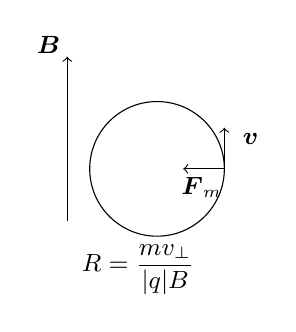
\begin{tikzpicture}[scale=0.95]
  \draw[->] (0,0) -- (0,2.2);
  \node at (-0.25,2.35) {\small \(\vb*{B}\)};
  \draw (1.2,0.7) circle (0.9);
  \draw[->] (2.1,0.7) -- (2.1,1.25);
  \node at (2.45,1.1) {\small \(\vb*{v}\)};
  \draw[->] (2.1,0.7) -- (1.55,0.7);
  \node at (1.8,0.45) {\small \(\vb*{F}_m\)};
  \node at (0.95,-0.65) {\small \(R=\dfrac{mv_\perp}{\abs{q}B}\)};
\end{tikzpicture}
\end{center}

\section{为什么磁力不做功}

磁力不做功的核心并不神秘，只来自一个几何事实：
\[
P=\vb*{F}_m\cdot \vb*{v}
=q(\vb*{v}\times \vb*{B})\cdot \vb*{v}=0.
\]
因为磁力永远垂直于瞬时速度，所以它不能直接增加或减少动能，只能改变速度方向。

\bridge{这句话非常值得反复咀嚼：\textbf{磁场最擅长做的事情不是“加速”粒子，而是“把粒子的运动方向掰弯”。} 以后你看到回旋加速器、质谱仪或电子束偏转，真正起作用的，首先都是“改方向”这一件事。}

\section{洛伦兹力的几个经典应用}

\textbf{速度选择器与质谱仪。} 若带电粒子同时进入互相垂直的电场和磁场，且初速度也与两者都垂直，则当
\[
qE=qvB
\]
时，电场力与磁场力恰好平衡，粒子不发生偏转，于是可选出满足
\[
v=\frac{E}{B}
\]
的那一束粒子。这就是\textbf{速度选择器}。若再让选速后的粒子进入仅有磁场 \(B_0\) 的分析区，它们会做半径为
\[
R=\frac{mv}{|q|B_0}
\]
的圆周运动，因此
\[
\frac{m}{|q|}=\frac{BB_0R}{E}.
\]
于是不同荷质比的粒子就会走出不同半径的轨道，这正是\textbf{质谱仪}区分同位素和测量荷质比的基本思想。

\textbf{汤姆孙实验与电子荷质比。} 阴极射线管中的电子先经电压 \(V\) 加速，因此
\[
\frac12 mv^2=eV.
\]
再让电子束进入互相垂直的电场和磁场，并调到屏上\textbf{不偏转}，则有
\[
eE=evB,
\qquad
v=\frac{E}{B}.
\]
联立两式便得
\[
\frac{e}{m}=\frac{E^2}{2VB^2}.
\]
这条链非常值得记住，因为它告诉你：\textbf{只要能独立控制加速电压、电场和磁场，就能把不可见电子的荷质比测出来。}

\textbf{回旋加速器。} 非相对论带电粒子在匀强磁场中的回旋频率
\[
f=\frac{|q|B}{2\pi m}
\]
与速率无关。因此，只要在两个 D 形盒的缝隙间施加同频交变电场，粒子每次经过缝隙都会被\textbf{电场}再次加速，而\textbf{磁场}只负责把它弯回下一次加速位置。若 D 形盒最大半径为 \(R_0\)，则离开加速器前的最大速率与最大动能约为
\[
v_{\max}=\frac{|q|BR_0}{m},
\qquad
E_{k,\max}=\frac{q^2B^2R_0^2}{2m}.
\]
这里最容易记反的一点是：\textbf{回旋加速器真正负责“增能”的是缝隙中的交变电场，不是磁场。} 磁场只改方向，不改动能。还要注意，这套“频率与速率无关”的结论只在非相对论范围内成立；当粒子速度太高时，相对论效应会让同步条件逐渐失配。

\textbf{磁聚焦（磁透镜）。} 若一束带电粒子从同一点出发，速率近似相同，但与 \(\vb*{B}\) 的夹角 \(\theta\) 都较小且略有差别，那么每个粒子都沿螺旋线前进，其节距为
\[
d=v_\parallel T
=v\cos\theta\frac{2\pi m}{|q|B}.
\]
当 \(\theta\) 都不大时，\(\cos\theta\) 变化不大，各条螺旋线的节距就近似相同，于是粒子束会在后方某处再次会聚。这个现象叫\textbf{磁聚焦}，其本质就是利用洛伦兹力把电子束“整形成像”，所以它在\textbf{电子光学、电子显微镜和电子束控制}中非常重要。

\textbf{霍耳效应。} 在载流导体或半导体中，载流子带着漂移速度 \(v_d\) 前进。若外加磁场垂直于电流方向，载流子会受到横向洛伦兹力，直到横向静电场建立起来并满足
\[
|q|E_H=|q|v_dB,
\qquad
E_H=v_dB.
\]
若试样宽度为 \(b\)、厚度为 \(d\)，则横向霍耳电压大小为
\[
|U_H|=E_Hb=v_dBb.
\]
再由电流大小
\[
I=n|q|v_dbd
\]
可得
\[
|U_H|=\frac{IB}{n|q|d}.
\]
若把载流子电荷符号一并计入霍耳系数，则常写成
\[
U_H=R_H\frac{IB}{d},
\qquad
R_H=\frac{1}{nq}.
\]
因此 \(R_H\) 的\textbf{符号}可以判断主要载流子是正电还是负电，\(R_H\) 的\textbf{大小}又能反推出载流子浓度，霍耳效应也常被用来测磁场。

\section{磁场对载流导线的作用}

导线里有大量定向运动的电荷，所以磁场对载流导线也会施力。若一小段导线元为 \(d\vb*{l}\)，电流为 \(I\)，则
\[
d\vb*{F}=I\,d\vb*{l}\times \vb*{B}.
\]
若导线为直导线且处在匀强磁场中，则总力可简化为
\[
\vb*{F}=I\vb*{L}\times \vb*{B},
\qquad
F=ILB\sin\theta.
\]
更一般地，任意一段平面载流导线在匀强磁场中的总力只与起点和终点有关：
\[
\vb*{F}
=I\int d\vb*{l}\times \vb*{B}
=I(\vb*{r}_{\mathrm{end}}-\vb*{r}_{\mathrm{start}})\times \vb*{B}.
\]
于是闭合线圈满足 \(\vb*{r}_{\mathrm{end}}=\vb*{r}_{\mathrm{start}}\)，总力自然为零；这也正是为什么线圈在匀强磁场里更典型的表现不是整体平移，而是受力矩。

这里本质上仍然是洛伦兹力的集体效果：导线中每个载流子都受磁场作用，把这些微观作用沿导线加总，便得到宏观载流导线的受力结果。

\begin{remark}
两根平行载流长直导线之间还会彼此作用：同向电流相吸，反向电流相斥。这个现象本质上就是“一个电流建立磁场，再去作用另一个电流”。
\end{remark}

\section{线圈为什么会被磁场“拧转”}

单根直导线在匀强磁场里往往表现为平移受力；但闭合线圈在匀强磁场里更典型的表现是\textbf{受力矩}。对面积为 \(S\)、电流为 \(I\)、法向单位矢量为 \(\vb*{n}\) 的线圈，定义磁矩
\[
\vb*{m}=IS\vb*{n}.
\]
它在匀强磁场中受到的力矩为
\[
\vb*{M}=\vb*{m}\times \vb*{B},
\qquad
M=mB\sin\theta.
\]
若线圈有 \(N\) 匝，则
\[
M=NISB\sin\theta.
\]
这里 \(\theta\) 是线圈法向 \(\vb*{n}\) 与磁场 \(\vb*{B}\) 的夹角，所以 \(\theta=0\) 时是稳定平衡，\(\theta=\pi\) 时是不稳定平衡，\(\theta=\pi/2\) 时力矩最大。

因此线圈总会倾向于把自己的磁矩方向转到与外磁场同向的位置。这个结果和电偶极子在匀强电场中受到力矩非常相似：那边是电偶极矩 \(\vb*{p}\) 想对准 \(\vb*{E}\)，这边是磁矩 \(\vb*{m}\) 想对准 \(\vb*{B}\)。

\begin{remark}
对匀强磁场中的闭合刚性平面线圈，\textbf{合力为零、合力矩一般不为零}。这两个结论要配套记：前者告诉你线圈不必整体飞走，后者告诉你它会被“拧转”到磁矩与外磁场同向的位置。
\end{remark}

\section{磁力对电流回路做功怎样和磁通接起来}

对恒定电流的闭合回路，不论它是在磁场中平移、转动还是缓慢形变，磁力或磁力矩所做的功都可写成
\[
A=I\Delta\Phi_B.
\]
若把线圈在匀强磁场中的转动拿来做例子，就有
\[
dA=M\,d\theta=IBS\sin\theta\,d\theta
=I\,d(BS\cos\theta)
=I\,d\Phi_B.
\]
这条关系非常重要，因为它把“磁力学里的受力矩”自然接到了下一章“磁通变化与感应电动势”的主线。以后你看到回路姿态改变时，除了想受力方向，也要开始想穿过它的磁通怎样变。

\section{例题精讲}

\begin{example}[任意平面载流导线在匀强磁场中的总受力]
在 \(xy\) 平面内，一段任意形状的平滑导线从 \(O(0,0)\) 延伸到 \(P(L,0)\)，导线中通有电流 \(I\)。空间存在垂直纸面向里的匀强磁场 \(\vb*{B}=-B\vb*{k}\)。求整段导线所受总磁场力。
\end{example}

\begin{solution}
这题最值得学的不是某个特殊曲线怎么积，而是一个更强的结论：\textbf{在匀强磁场中，平面载流导线的总受力只由始点、终点决定。}

设电流元
\[
d\vb*{l}=dx\,\vb*{i}+dy\,\vb*{j}.
\]
则安培力微元为
\[
d\vb*{F}=I\,d\vb*{l}\times \vb*{B}
=I(dx\,\vb*{i}+dy\,\vb*{j})\times(-B\vb*{k}).
\]
逐项叉乘得
\[
d\vb*{F}=BI\,dx\,\vb*{j}-BI\,dy\,\vb*{i}.
\]
于是
\[
dF_x=-BI\,dy,\qquad dF_y=BI\,dx.
\]
沿整条导线积分：
\[
F_x=-BI\int_O^P dy=0,
\]
因为起点和终点的 \(y\) 坐标都为 \(0\)；
\[
F_y=BI\int_O^P dx=BIL,
\]
因为从 \(x=0\) 走到 \(x=L\)。

故总磁场力为
\[
\vb*{F}=BIL\,\vb*{j}.
\]
也就是说，它恰好等于那根\textbf{从 \(O\) 直连到 \(P\) 的直导线}在同一匀强磁场中所受的力。这是很多安培力积分题里最省力的捷径之一。
\end{solution}

\begin{example}[圆形线圈在匀强磁场中的力矩与做功]
半径为 \(R\) 的单匝圆形线圈中通有电流 \(I\)。将它放入匀强磁场中，且初始时磁场方向与线圈平面平行。求：
\begin{enumerate}
  \item 初始时线圈所受磁力矩的大小；
  \item 若线圈在磁力矩作用下转到法向与 \(\vb*{B}\) 同向，磁场力共做多少功。
\end{enumerate}
\end{example}

\begin{solution}
对闭合平面线圈，最稳的入口不是逐段算力，而是直接用磁矩
\[
\vb*{m}=IS\,\vb*{n},
\qquad
S=\pi R^2.
\]
初始时磁场与线圈平面平行，故它与法向 \(\vb*{n}\) 的夹角为 \(90^\circ\)。因此总磁力矩大小为
\[
M=mB\sin 90^\circ
=IB\pi R^2.
\]

再看做功。线圈转动时，若电流保持不变，磁力矩所做的功可写成
\[
A=I\Delta\Phi_B.
\]
初始时磁通量
\[
\Phi_i=BS\cos 90^\circ=0,
\]
末态时线圈法向与磁场同向，
\[
\Phi_f=BS\cos 0^\circ=BS=B\pi R^2.
\]
故
\[
A=I(\Phi_f-\Phi_i)=IB\pi R^2.
\]

这题里力矩大小和总做功恰好写成了同一个系数 \(IB\pi R^2\)，但它们的物理意义完全不同：前者是某一姿态下的“转动趋势”，后者是整个转动过程中“累计转移的能量”。
\end{solution}

\begin{example}[长直载流导线在匀强磁场中的受力]
一段长为 \(L\) 的直导线中通有电流 \(I\)，置于匀强磁场 \(\vb*{B}\) 中。若导线方向与磁场夹角为 \(\theta\)，求导线所受安培力。
\end{example}

\begin{solution}
对直导线，安培力微元
\[
d\vb*{F}=I\,d\vb*{l}\times \vb*{B}.
\]
由于整段导线方向固定、磁场又均匀，大小可以直接积出来：
\[
F=\int I B\sin\theta\,dl
=IB\sin\theta\int_0^L dl.
\]
因此
\[
\boxed{F=ILB\sin\theta}.
\]
方向由 \(I\vb*{L}\times \vb*{B}\) 决定。这个式子其实就是安培力最常见的整段导线版，后面很多复杂导线题都只是把它拆回微元再积分。
\end{solution}

\begin{example}[有限长直导线受无限长直导线的磁场力]
一根无限长直导线中通有电流 \(I_1\)。与它共面地放置一根长为 \(L\) 的直导线，电流为 \(I_2\)。设该导线近端到长直导线的距离为 \(r\)，并与过近端的垂线夹角为 \(\alpha\)。求这根有限导线所受磁场力大小。
\end{example}

\begin{solution}
长直导线在距其 \(x\) 处产生的磁场大小为
\[
B(x)=\frac{\mu_0I_1}{2\pi x}.
\]
有限导线上的每一小段所受安培力方向相同，因此只需积分大小。由几何关系
\[
x=r+l\cos\alpha,
\qquad
dl=\frac{dx}{\cos\alpha}.
\]
于是
\[
dF=I_2B(x)\,dl
=\frac{\mu_0I_1I_2}{2\pi x}\frac{dx}{\cos\alpha}.
\]
从 \(x=r\) 积到 \(x=r+L\cos\alpha\)，得
\[
F=\frac{\mu_0I_1I_2}{2\pi\cos\alpha}\int_r^{r+L\cos\alpha}\frac{dx}{x}
=\frac{\mu_0I_1I_2}{2\pi\cos\alpha}\ln\frac{r+L\cos\alpha}{r}.
\]
故
\[
\boxed{
F=\frac{\mu_0I_1I_2}{2\pi\cos\alpha}\ln\frac{r+L\cos\alpha}{r}
}.
\]
这题的难点纯粹是几何变量替换，本质仍是“先找外磁场，再对安培力积分”。
\end{solution}

\begin{example}[半圆形载流导线在匀强磁场中的受力]
半径为 \(R\) 的半圆形导线位于纸面内，电流沿圆弧从左端流向右端，空间有垂直纸面向里的匀强磁场 \(B\)。求该半圆弧所受总安培力。
\end{example}

\begin{solution}
逐元积分固然可做，但更快的识别是：在匀强磁场中，一段平面载流导线的总受力只由起点和终点决定。因此该半圆弧受到的总力，等于连接两端的直径导线在同一磁场中的受力。

于是直接得
\[
F=IB(2R).
\]
故
\[
\boxed{F=2IBR}.
\]
方向由电流方向与磁场方向的叉乘决定；按题设取向，它与直径垂直并指向半圆开口一侧。这个结果很好地说明了“匀强磁场里算整段导线受力，别总想着沿曲线死积分”。
\end{solution}

\begin{example}[圆形线圈在指定坐标系中的磁力矩方向]
一半径为 \(R\) 的可转动圆形线圈中通有电流 \(I\)，线圈法向沿 \(+z\) 方向，匀强磁场 \(\vb*{B}=B\vb*{i}\)。求线圈所受磁力矩。
\end{example}

\begin{solution}
线圈磁矩为
\[
\vb*{m}=IS\,\vb*{k}=I\pi R^2\,\vb*{k}.
\]
所以
\[
\vb*{M}=\vb*{m}\times \vb*{B}
=I\pi R^2\,\vb*{k}\times B\vb*{i}
=I\pi R^2B\,\vb*{j}.
\]
故
\[
\boxed{\vb*{M}=I\pi R^2B\,\vb*{j}}.
\]
这题提醒我们：很多线圈受力矩题真正的关键不是大小，而是先把磁矩方向判对，再用叉乘一把得到方向。
\end{solution}

\begin{example}[圆电流与共面长直导线间的安培力]
一根无限长直导线与半径为 \(R\)、电流为 \(I\) 的圆电流共面放置，并沿圆的一条直径方向通过。长直导线电流为 \(I_0\)。求：
\begin{enumerate}
  \item 圆上半弧所受总安培力；
  \item 整个圆电流所受总安培力。
\end{enumerate}
\end{example}

\begin{solution}
对位于半圆弧上的电流元，长直导线在其处产生的磁场大小为
\[
B=\frac{\mu_0 I_0}{2\pi x},
\]
其中 \(x=R\sin\theta\)。把安培力微元分解后，由对称性可知垂直于直径的分量相互抵消，只剩沿直径方向的分量。积分结果为
\[
F_{\text{半弧}}=\frac{\mu_0 I_0 I}{2}.
\]
而对整个圆电流，同样的积分在上下两半圆上同向叠加，因此
\[
F_{\text{全圆}}=\mu_0 I_0 I.
\]
故
\[
\boxed{
F_{\text{半弧}}=\frac{\mu_0 I_0 I}{2},
\qquad
F_{\text{全圆}}=\mu_0 I_0 I.
}
\]
这类题看起来像“奇怪几何”，本质还是两步：先写出长直导线的磁场，再利用对称性删去会互相抵消的分量。
\end{solution}

\section{本章统一起手动作}

涉及磁场力时，最稳的顺序是：
\begin{enumerate}
  \item 先看研究对象：单个电荷、整段导线，还是闭合线圈；
  \item 再看 \(\vb*{v}\) 或 \(d\vb*{l}\) 与 \(\vb*{B}\) 的夹角；
  \item 然后先画方向图，再代数计算大小；
  \item 一旦题目问能量或速率变化，立刻回想“磁力不做功”，看它到底能改什么、不能改什么。
\end{enumerate}

\section{常见误区}

\begin{itemize}
  \item 把磁力方向错画成沿 \(\vb*{v}\) 或沿 \(\vb*{B}\)。
  \item 误以为“只要有磁力就一定会越来越快”。磁力改方向，不直接改动能。
  \item 把载流导线受力和平行导线相互作用混成两套无关公式，忘了它们都来自 \(I\,d\vb*{l}\times \vb*{B}\)。
  \item 看到线圈就只算总力，忽略真正支配转动的是力矩。
\end{itemize}

\section{章末小结}

\summaryline{磁场对运动电荷的作用由洛伦兹力给出，它总垂直于速度，所以最擅长“拐弯”而不是“增速”；速度选择器、质谱仪、汤姆孙实验、回旋加速器和霍耳效应都只是这同一条力学主线在不同装置中的展开；对载流导线，微观洛伦兹力加总成宏观磁场力；对闭合线圈，又进一步表现为磁矩在外磁场中的受力矩。}
\chapterselfcheck{为什么匀强磁场能让粒子做圆周或螺旋运动，却不直接改动能？为什么回旋加速器里真正负责增加动能的是电场而不是磁场？为什么霍耳电压的符号能判断载流子类型？遇到电子在磁场中偏转的题，为什么一定要先画方向图？}

\chapter{磁介质}

\chapterroadmap
{回答“物质进入磁场后怎样被磁化”，并把 \(\vb*{B},\vb*{H},\vb*{M}\) 三个量的分工理顺。}
{已经知道电流建立磁场、磁场作用于运动电荷和电流。}
{新增磁化、磁化电流、磁场强度 \(\vb*{H}\)、介质中的安培环路定理，以及抗磁/顺磁/铁磁的差异。}

\bridge{静电学里，电介质进入外场会极化；磁学里，磁介质进入外场会磁化。于是 \(\vb*{B}\) 不再只由自由电流决定，还会受到介质内部微观磁矩取向变化的影响。学这一章的关键，就是把“自由电流造的那部分场”和“介质自己响应出来的那部分场”分开记账。}

\section{磁化与磁矩}

从微观上看，很多原子、分子或电子轨道本身就可等效为小电流环，于是带有磁矩。没有外磁场时，这些微观磁矩往往取向杂乱，宏观平均后磁效应不明显；加上外磁场后，部分磁矩趋于定向排列，宏观上就表现为磁化。

磁化强度记作 \(\vb*{M}\)，它描述单位体积内净磁矩的平均分布。虽然教材上它看起来只是“又一个新矢量”，但物理意义非常明确：\textbf{它刻画的是介质内部自己贡献出来的磁性部分。}

\bridge{若把磁化想成大量微观小电流环重新排队，就会发现一个很关键的几何事实：相邻小电流环在内部边界上的电流会彼此抵消，真正留下来的主要是外表面的等效环流。因此磁化不仅可以用“磁矩取向”来讲，也可以用“等效磁化电流”来讲。}

若取一条闭合回路 \(L\) 围住介质的一部分，则磁化强度与等效磁化电流满足
\[
\oint_L \vb*{M}\cdot d\vb*{l}=\sum I_s,
\]
这里 \(\sum I_s\) 表示被回路围住的等效磁化电流代数和。这个关系的价值在于：它把抽象的 \(\vb*{M}\) 重新翻译回了我们已经熟悉的“电流造磁场”语言。

\section{磁场强度 H 与介质中的安培环路定理}

为了把“自由电流贡献”和“磁化贡献”分账，引入磁场强度 \(\vb*{H}\)。在真空中，
\[
\vb*{B}=\mu_0\vb*{H};
\]
在一般介质中，
\[
\vb*{B}=\mu_0(\vb*{H}+\vb*{M}).
\]
这并不是凭空定义出来的，而是来自介质中总环量的分账：
\[
\oint_L \vb*{B}\cdot d\vb*{l}
=\mu_0\left(\sum I_{\mathrm{free}}+\sum I_s\right)
=\mu_0\left(\sum I_{\mathrm{free}}+\oint_L \vb*{M}\cdot d\vb*{l}\right).
\]
把 \(\oint_L \vb*{M}\cdot d\vb*{l}\) 移到左边，就自然引出
\[
\vb*{H}=\frac{\vb*{B}}{\mu_0}-\vb*{M},
\qquad
\oint_L \vb*{H}\cdot d\vb*{l}=I_{\mathrm{free}}.
\]
对各向同性线性均匀磁介质，还可以进一步写成
\[
\vb*{M}=\chi_m \vb*{H},
\qquad
\vb*{B}=\mu\vb*{H},
\]
其中 \(\mu=\mu_0(1+\chi_m)\) 为磁导率。

于是安培环路定理在介质中最实用的写法变成
\[
\oint_L \vb*{H}\cdot d\vb*{l}=I_{\mathrm{free}}.
\]

\begin{note}
\textbf{这和电介质里引入 \(\vb*{D}\) 的思路完全平行：} \(\vb*{B}\) 对总磁效应负责，\(\vb*{H}\) 主要对自由电流负责。以后只要介质一出现，就不要再把真空中的单一本构关系机械照搬。
\end{note}

\section{三类常见磁介质：抗磁、顺磁、铁磁}

\begin{itemize}
  \item \textbf{抗磁质：} 外场使感生磁矩方向与外场相反，磁化很弱，\(\mu_r\) 略小于 1。
  \item \textbf{顺磁质：} 原有磁矩在外场中略趋同向，磁化较弱，\(\mu_r\) 略大于 1。
  \item \textbf{铁磁质：} 内部存在磁畴结构，外场可使磁畴大范围重排，因此磁化很强，\(\mu_r\) 可远大于 1。
\end{itemize}

铁磁质之所以特殊，不只是“磁化更大”，而是它具有明显的历史效应：外场撤去后，磁化不一定立刻完全消失，于是出现剩磁、矫顽力和磁滞回线等现象。

\section{磁滞与软磁、硬磁材料}

铁磁材料里，\(\vb*{B}\) 与 \(\vb*{H}\) 之间常不再是一条简单直线，而是随加磁、退磁历史出现磁滞回线。回线窄、矫顽力小的材料适合做铁芯等反复磁化退磁的器件，常称\textbf{软磁材料}；回线宽、剩磁大的材料适合做永久磁体，常称\textbf{硬磁材料}。

\begin{remark}
这里最容易被忽略的是：铁磁质不是“\(\mu\) 特别大”的单纯线性介质，而是一类具有磁畴结构、非线性和历史记忆效应的材料。
\end{remark}

\section{例题精讲}

\begin{example}[\(H\) 与 \(B\) 的分段分工]
一半径为 \(R_1\) 的无限长圆柱导线外包一层外半径为 \(R_2\)、相对磁导率为 \(\mu_r\) 的均匀磁介质圆筒。导线中通有电流 \(I\)，且电流在导线截面上均匀分布。求各区域中的磁场强度 \(H(r)\) 与磁感应强度 \(B(r)\)。
\end{example}

\begin{solution}
这题最关键的观念不是一上来就算 \(B\)，而是先记住：\textbf{\(\vb*{H}\) 主要由自由电流决定，\(\vb*{B}\) 再由介质响应放大或缩小。}

先用半径为 \(r\) 的圆形安培回路。由对称性，\(\vb*{H}\) 沿回路切向且大小恒定，于是
\[
\oint \vb*{H}\cdot d\vb*{l}=H(2\pi r)=I_{\mathrm{free,enc}}.
\]

当 \(0<r<R_1\) 时，包围的自由电流仅占总电流的面积比：
\[
I_{\mathrm{enc}}=I\frac{r^2}{R_1^2}.
\]
故
\[
H(r)=\frac{Ir}{2\pi R_1^2},
\qquad
B(r)=\mu_0H(r)=\frac{\mu_0Ir}{2\pi R_1^2}.
\]
这里仍在导线本体内部，尚未进入外包磁介质，所以 \(B=\mu_0H\)。

当 \(R_1<r<R_2\) 时，回路已包围全部自由电流 \(I\)，因此
\[
H(r)=\frac{I}{2\pi r}.
\]
但这一区域位于磁介质中，所以
\[
B(r)=\mu H(r)=\mu_0\mu_r\frac{I}{2\pi r}.
\]

当 \(r>R_2\) 时，回路外侧回到真空（或空气），包围自由电流仍是 \(I\)，所以
\[
H(r)=\frac{I}{2\pi r},
\qquad
B(r)=\mu_0\frac{I}{2\pi r}.
\]

综上，
\[
H(r)=
\begin{cases}
\dfrac{Ir}{2\pi R_1^2}, & 0<r<R_1,\\[6pt]
\dfrac{I}{2\pi r}, & r>R_1,
\end{cases}
\]
\[
B(r)=
\begin{cases}
\dfrac{\mu_0Ir}{2\pi R_1^2}, & 0<r<R_1,\\[6pt]
\dfrac{\mu_0\mu_rI}{2\pi r}, & R_1<r<R_2,\\[6pt]
\dfrac{\mu_0I}{2\pi r}, & r>R_2.
\end{cases}
\]

这正体现了 \(\vb*{H}\) 与 \(\vb*{B}\) 的分工：\(\vb*{H}\) 先把自由电流的“源账”做好，\(\vb*{B}\) 再通过不同区域的本构关系体现介质影响。
\end{solution}

\begin{example}[充满磁介质的长直螺线管]
一长直密绕螺线管内充满相对磁导率为 \(\mu_r\) 的均匀磁介质，单位长度匝数为 \(n\)，通有电流 \(I\)。求管内磁感应强度。
\end{example}

\begin{solution}
先对 \(\vb*{H}\) 用安培环路定理。取一条跨越螺线管内外的矩形回路，由于长螺线管外部磁场近似很小，内部 \(\vb*{H}\) 近似均匀，故
\[
Hl=nIl
\quad\Longrightarrow\quad
H=nI.
\]
再由线性磁介质中的本构关系
\[
B=\mu H=\mu_0\mu_r H
\]
得到
\[
\boxed{
B=\mu_0\mu_r nI
}.
\]
这题最能说明“先算 \(H\)，再转成 \(B\)”的好处：自由电流决定 \(H\)，介质参数只在最后一步进入。
\end{solution}

\begin{example}[两同轴反向电流圆筒间的磁场]
有两个半径分别为 \(R_1,R_2\) 的无限长同轴圆筒形导体，之间充满相对磁导率为 \(\mu_r\) 的均匀磁介质。两圆筒中通有大小相等、方向相反的电流 \(I\)。求各区域磁感应强度。
\end{example}

\begin{solution}
对三段区域分别用安培环路定理求 \(\vb*{H}\)：

当 \(r<R_1\) 时，回路不包围净自由电流，故
\[
H=0,\qquad B=0.
\]

当 \(R_1<r<R_2\) 时，回路只包围内圆筒电流 \(I\)，故
\[
H\cdot 2\pi r=I
\quad\Longrightarrow\quad
H=\frac{I}{2\pi r}.
\]
此区在磁介质内，所以
\[
B=\mu_0\mu_r H
=\frac{\mu_0\mu_r I}{2\pi r}.
\]

当 \(r>R_2\) 时，回路同时包围 \(+I\) 和 \(-I\)，净自由电流为零，因此
\[
H=0,\qquad B=0.
\]
故
\[
\boxed{
B(r)=
\begin{cases}
0, & r<R_1,\\[4pt]
\dfrac{\mu_0\mu_r I}{2\pi r}, & R_1<r<R_2,\\[6pt]
0, & r>R_2.
\end{cases}}
\]
它和同轴电缆的电场分布非常像，只不过这里是磁场，而且由反向电流把场锁在两圆筒之间。
\end{solution}

\section{本章统一起手动作}

磁介质题最稳的起手顺序通常是：
\begin{enumerate}
  \item 先问题目是在\textbf{算场}，还是在\textbf{认材料行为}；
  \item 若是算场，先把自由电流与介质响应分账：优先用
  \[
  \oint \vb*{H}\cdot d\vb*{l}=I_{\mathrm{free}}
  \]
  去锁自由电流贡献，再回到 \(\vb*{M}\) 与 \(\vb*{B}\)；
  \item 若介质可近似看作线性、各向同性、均匀介质，就顺着
  \[
  \vb*{M}=\chi_m\vb*{H},
  \qquad
  \vb*{B}=\mu\vb*{H}
  \]
  这条链往下走；
  \item 若题目谈的是铁磁质、磁滞、剩磁、矫顽力，就不要再把它当成“\(\mu\) 很大的线性材料”，而应切到磁畴与历史效应的语言。
\end{enumerate}

\begin{note}
\textbf{这一章最值得死记的不是某个单独公式，而是三者分工：} \(\vb*{B}\) 描写总磁效应，\(\vb*{H}\) 主要对自由电流记账，\(\vb*{M}\) 描写介质自己的磁化响应。很多介质题一旦把这三者混成一个量，后面几乎必乱。
\end{note}

\section{常见误区}

\begin{itemize}
  \item 把 \(\vb*{B}\) 和 \(\vb*{H}\) 当成同一个量，只差一个单位。
  \item 在介质题里仍然机械使用真空关系 \(B=\mu_0H\)。
  \item 以为顺磁、抗磁、铁磁的区别只是“强弱不同”，忽略铁磁质的磁畴和磁滞特性。
  \item 以为磁化意味着材料内部真的有宏观电荷流在绕圈跑；更准确地说，它是微观磁矩平均取向变化的宏观表述。
\end{itemize}

\section{章末小结}

\summaryline{磁介质进入外磁场后会磁化，于是磁场分成“自由电流建立的部分”和“介质响应建立的部分”两本账。用 \(\vb*{H}\) 可以更方便地追踪前者，用 \(\vb*{M}\) 则描述后者；而铁磁质之所以特殊，关键在于磁畴重排和磁滞。}
\chapterselfcheck{为什么介质题里要把 \(\vb*{B}\)、\(\vb*{H}\)、\(\vb*{M}\) 分开？为什么铁磁质不能简单看成“\(\mu\) 很大的线性介质”？为什么介质中的安培环路定理更适合写成关于 \(\vb*{H}\) 的形式？}

\chapter{电磁感应}

\chapterroadmap
{把“变化的磁场”与“感应电动势”接起来，理解法拉第定律、楞次定律、动生/感生电动势，以及自感、互感和磁场能量。}
{已经会描述稳恒电流和静磁场，也知道磁场对电荷和电流的作用。}
{新增磁通量、法拉第电磁感应定律、非静电力场、自感/互感与磁场能量。}

\bridge{前面磁学讨论的大多是“电流产生磁场、磁场作用电流”；这一章出现真正的双向耦合：变化的磁场反过来又能生电场和电流。法拉第定律因此是电磁学从“静态章节并列”走向“动态统一理论”的关键转折。}

\section{磁通量与法拉第电磁感应定律}

穿过某曲面的磁通量定义为
\[
\Phi_B=\int_S \vb*{B}\cdot d\vb*{S}.
\]
若回路所围曲面的磁通量随时间变化，则回路中会出现感应电动势：
\[
\mathcal{E}=-\dv{\Phi_B}{t}.
\]
这就是\textbf{法拉第电磁感应定律}。

这里的负号不是装饰，而是\textbf{楞次定律}的数学体现：感应电流总要反抗原磁通变化。若原磁通在增大，感应电流建立的磁场就倾向于让它减小；若原磁通在减小，感应电流就倾向于把它“补回来”。

\begin{remark}
真正判断方向时，最稳的做法是：\textbf{先任选回路绕行方向，再按右手螺旋给穿过回路的磁通规定正方向。} 若算得 \(\mathcal{E}>0\)，说明感应电动势方向与所选绕向一致；若算得 \(\mathcal{E}<0\)，则实际方向与所选绕向相反。这样负号就不再神秘，而是清楚地落实到方向约定上。
\end{remark}

若线圈有 \(N\) 匝，更自然的记账量是\textbf{磁通链}
\[
\Psi=N\Phi_B,
\qquad
\mathcal{E}=-\dv{\Psi}{t}.
\]

\section{动生电动势与感生电动势}

磁通变化有两种典型来源：
\begin{itemize}
  \item 回路本身在磁场中运动或形变，这时常称\textbf{动生电动势}；
  \item 回路不动，但空间磁场随时间变化，这时常称\textbf{感生电动势}。
\end{itemize}

对长度为 \(l\) 的金属棒以速度 \(v\) 垂直切割匀强磁场时，有经典结果
\[
\mathcal{E}=Blv.
\]
更一般地，动生电动势可写成
\[
\mathcal{E}=\int (\vb*{v}\times \vb*{B})\cdot d\vb*{l}.
\]
而感生电动势的本质，则是变化磁场激发了非静电感应电场，使得沿闭合回路
\[
\oint \vb*{E}_{\mathrm{ind}}\cdot d\vb*{l}=-\dv{\Phi_B}{t}.
\]

\begin{example}
设半径为 \(R\) 的长螺线管内部磁场 \(B(t)\) 近似均匀，管外磁场近似忽略。若取与轴同心、半径为 \(r\) 的圆形回路，则感生电场沿环向分布，并满足
\[
2\pi r E_\varphi=-\pi r^2\dv{B}{t},
\qquad r<R,
\]
故
\[
E_\varphi(r)=-\frac{r}{2}\dv{B}{t}.
\]
若 \(r>R\)，穿过回路的磁通只由半径 \(R\) 的内部磁场决定，于是
\[
2\pi r E_\varphi=-\pi R^2\dv{B}{t},
\qquad
E_\varphi(r)=-\frac{R^2}{2r}\dv{B}{t}.
\]
这说明感生电场并不只存在于“有磁场的地方”，而是以闭合场线的形式分布在更广的空间区域中。换句话说，它的电场线不是从正电荷出发、到负电荷终止，而是绕着变化磁通围成一圈圈与螺线管同轴的闭合同心圆。
\end{example}

\begin{remark}
动生电动势的“非静电力来源”可以直接追到洛伦兹力；感生电动势则更深一步，说明即使没有导体整体运动，变化磁场本身也能在空间中建立有旋电场。
\end{remark}

\begin{remark}
也正因为感生电场本身就真实存在，所以即使导体整体静止、甚至不是完整闭合回路，导体两端也可能测得感应电动势；若把大块导体放入时变磁场中，内部还会自动围成许多闭合感应电流回路，这就是\textbf{涡电流}。它一方面会带来额外焦耳热，另一方面又能产生电磁阻尼，所以工程上常通过叠片、开槽等方式削弱涡流回路面积。
\end{remark}

\section{自感与互感}

如果同一回路中的电流变化引起本回路磁通变化，就会在自身回路中产生感应电动势，这叫\textbf{自感}。更严谨地说，应先定义磁通链 \(\Psi\)，再写
\[
\Psi=LI,
\qquad
\mathcal{E}_L=-L\dv{I}{t}.
\]
若线圈有 \(N\) 匝，则 \(\Psi=N\Phi_B\)。只有在单匝或已默认按磁通链记账时，才可把它简写成“\(\Phi\) 与 \(I\) 成正比”的样子。

若一个回路中的电流变化，引起另一个回路中磁通变化并产生感应电动势，则叫\textbf{互感}。同样应先写成
\[
\Psi_{21}=MI_1,
\qquad
\mathcal{E}_{21}=-M\dv{I_1}{t}.
\]

\begin{note}
自感和互感的核心物理意义都是“电流变化引起磁通变化，再由磁通变化反过来阻碍这种变化”。这也是为什么很多电感元件表现出“电流不愿突然变化”的惯性。
\end{note}

\section{磁场能量}

建立电流要克服自感电动势，因此外界做功会储存在磁场中。对电感元件，
\[
W_m=\frac{1}{2}LI^2.
\]
若进一步写成场的形式，在真空中常用
\[
w_m=\frac{B^2}{2\mu_0},
\]
在一般线性介质中则更自然地写成
\[
w_m=\frac{1}{2}\vb*{B}\cdot \vb*{H}.
\]

\bridge{电场里有 \(\frac12 \vb*{E}\cdot \vb*{D}\)，磁场里有 \(\frac12 \vb*{B}\cdot \vb*{H}\)。这再次提醒我们：电磁学越来越倾向于把能量理解成\textbf{场分布}，而不是只贴在元件或粒子本身。}

\section{例题精讲}

\begin{example}[滑动导杆的感应电动势]
矩形闭合导体回路的一边 \(ab\) 长为 \(l\)，可在导轨上无摩擦滑动。整个回路处在垂直于回路平面、大小为 \(B\) 的匀强磁场中。若导杆 \(ab\) 以恒定速度 \(v\) 向右滑动，求回路中的感应电动势。
\end{example}

\begin{solution}
这类题最稳的入口不是背 \(Blv\)，而是先把它翻译成“\textbf{磁通为什么在变}”。这里 \(B\) 不变，夹角不变，真正变化的是回路面积。

设时刻 \(t\) 时导杆位置对应回路宽度为 \(x\)，取顺时针绕行为正，则穿过回路的磁通量为
\[
\Phi_B=BS=Blx.
\]
于是
\[
\mathcal{E}=-\dv{\Phi_B}{t}
=-Bl\dv{x}{t}
=-Blv.
\]

所以感应电动势大小为
\[
\abs{\mathcal{E}}=Blv.
\]
负号表示：若我们把顺时针取作正方向，那么真实感应电流方向与之相反，即为\textbf{逆时针方向}。这和楞次定律完全一致，因为导杆右移使回路面积增大，原磁通增强，于是感应电流必须建立一个反抗这种增强的磁场。
\end{solution}

\begin{example}[时变长直电流在线圈中激发的感应电动势]
一根无限长直导线中通有电流
\[
i(t)=I_0\sin\omega t.
\]
导线旁有一个与之共面的矩形线圈，线圈靠近导线的一边距导线为 \(r\)，沿径向宽度为 \(l_1\)，沿导线方向长度为 \(l_2\)。求线圈中的感应电动势。
\end{example}

\begin{solution}
长直导线在距其 \(x\) 处产生的磁场大小为
\[
B(x,t)=\frac{\mu_0 i(t)}{2\pi x}
=\frac{\mu_0 I_0\sin\omega t}{2\pi x}.
\]
矩形线圈中每条与导线平行的窄条面积元可写成
\[
dS=l_2\,dx,
\]
故穿过线圈的总磁通为
\[
\Phi_B
=\int_r^{r+l_1} B(x,t)\,l_2\,dx
=\frac{\mu_0 I_0l_2}{2\pi}\sin\omega t
\int_r^{r+l_1}\frac{dx}{x}.
\]
于是
\[
\Phi_B
=\frac{\mu_0 I_0l_2}{2\pi}\ln\frac{r+l_1}{r}\,\sin\omega t.
\]
对时间求导即得感应电动势：
\[
\mathcal{E}
=-\dv{\Phi_B}{t}
=-\frac{\mu_0 I_0l_2\omega}{2\pi}\ln\frac{r+l_1}{r}\,\cos\omega t.
\]

这个结果特别适合拿来训练“磁通变化来源”的辨认：这里面积不变、姿态不变、线圈不动，\textbf{唯一在变的是源电流，从而磁场随时间变。} 一旦识别出这点，后面就是“先求磁通，再对时间求导”的固定套路。
\end{solution}

\begin{example}[运动矩形线框在长直电流磁场中的感应电动势]
一矩形导体线框与一根无限长直导线共面。线框沿垂直于长直导线的方向平移，靠近导线一边到导线的距离为 \(l\)，线框宽为 \(a\)、高为 \(b\)，平移速度为 \(v\)。长直导线中电流恒为 \(I\)。求线框中的感应电动势。
\end{example}

\begin{solution}
长直导线在距其 \(x\) 处的磁场为
\[
B(x)=\frac{\mu_0I}{2\pi x}.
\]
所以线框中的磁通量为
\[
\Phi_B=\int_l^{l+a}\frac{\mu_0I}{2\pi x}b\,dx
=\frac{\mu_0Ib}{2\pi}\ln\frac{l+a}{l}.
\]
由于线框在运动，\(l=l(t)\) 且 \(\dot l=v\)。因此
\[
\mathcal{E}=-\dv{\Phi_B}{t}
=-\frac{\mu_0Ib}{2\pi}\dv{}{t}\left(\ln\frac{l+a}{l}\right)
=\frac{\mu_0Iabv}{2\pi l(l+a)}.
\]
故
\[
\boxed{
\mathcal{E}=\frac{\mu_0Iabv}{2\pi l(l+a)}
}.
\]
方向由楞次定律判断：若线框远离导线，原磁通减小，则感应电流要设法维持原磁通方向。
\end{solution}

\begin{example}[转动导体棒两端的动生电动势]
一根长为 \(L\) 的导体棒在垂直于磁场 \(B\) 的平面内绕一端以角速度 \(\omega\) 匀速转动。求棒两端之间的动生电动势大小。
\end{example}

\begin{solution}
把导体棒分成距转轴为 \(l\) 的小段。该处线速度
\[
v=\omega l,
\]
所以小段上产生的动生电动势元为
\[
d\mathcal{E}=Bv\,dl=B\omega l\,dl.
\]
从 \(0\) 积到 \(L\)：
\[
\mathcal{E}=\int_0^L B\omega l\,dl
=\frac12 B\omega L^2.
\]
故
\[
\boxed{
\mathcal{E}=\frac12 B\omega L^2
}.
\]
方向由右手定则判断：若磁场垂直纸面向里、棒逆时针转动，则正电荷被推向外端。
\end{solution}

\begin{example}[长直导线旁移动金属棒的动生电动势]
一根长直导线中通恒定电流 \(I\)。一根长度为 \(l\) 的金属棒与导线垂直、并与导线共面，近端到导线距离为 \(a\)。若金属棒以速度 \(v\) 平行于长直导线匀速运动，求棒两端的动生电动势。
\end{example}

\begin{solution}
长直导线在距其 \(x\) 处的磁场为
\[
B(x)=\frac{\mu_0I}{2\pi x}.
\]
动生电动势沿棒积分：
\[
\mathcal{E}=\int_a^{a+l}(\vb*{v}\times\vb*{B})\cdot d\vb*{l}
=v\int_a^{a+l}B(x)\,dx.
\]
代入 \(B(x)\)：
\[
\mathcal{E}
=\frac{\mu_0Iv}{2\pi}\int_a^{a+l}\frac{dx}{x}
=\frac{\mu_0Iv}{2\pi}\ln\frac{a+l}{a}.
\]
故
\[
\boxed{
\mathcal{E}=\frac{\mu_0Iv}{2\pi}\ln\frac{a+l}{a}
}.
\]
这里最容易错的是把 \(B\) 当常量；实际上棒上不同位置离长直导线远近不同，磁场并不均匀。
\end{solution}

\begin{example}[磁场中的导体棒为何会指数减速]
一根长为 \(l\)、质量为 \(m\) 的导体棒在匀强磁场 \(B\) 中沿导轨运动，并与总电阻为 \(R\) 的回路相连。若初速度为 \(v_0\)，求它的速度随时间的变化规律。
\end{example}

\begin{solution}
棒运动时产生感应电动势
\[
\mathcal{E}=Blv,
\]
故回路电流为
\[
I=\frac{\mathcal{E}}{R}=\frac{Blv}{R}.
\]
导体棒所受安培力大小
\[
F=BIl=\frac{B^2l^2}{R}v,
\]
方向总与运动方向相反，因此
\[
m\dv{v}{t}=-\frac{B^2l^2}{R}v.
\]
分离变量积分得
\[
v(t)=v_0\exp\left(-\frac{B^2l^2}{mR}t\right).
\]
所以
\[
\boxed{
v(t)=v_0e^{-B^2l^2t/(mR)}
}.
\]
这题非常值得拿来理解楞次定律的动力学含义：感应电流总会以反抗原运动的方式“吃掉”机械能。
\end{solution}

\begin{example}[折线导线的动生电动势为何等于两端弦线]
一根形状任意的刚性导线 \(abc\) 在匀强磁场中整体平移。说明其动生电动势为什么只取决于端点，等于连接两端的直导线 \(ac\) 的动生电动势。
\end{example}

\begin{solution}
把导线 \(abc\) 与一根假想直导线 \(ca\) 拼成闭合刚性回路 \(abca\)。由于整个刚性回路都以同一速度平移、回路面积不变、磁通不变，因此
\[
\mathcal{E}_{abca}=0.
\]
又因为
\[
\mathcal{E}_{abca}=\mathcal{E}_{abc}+\mathcal{E}_{ca},
\]
所以
\[
\mathcal{E}_{abc}=-\mathcal{E}_{ca}=\mathcal{E}_{ac}
\]
（方向按同一约定处理）。因此
\[
\boxed{\mathcal{E}_{abc}=\mathcal{E}_{ac}}.
\]
这说明在匀强磁场中的整体平移问题里，动生电动势具有明显的“端点决定”特征。
\end{solution}

\begin{example}[长直螺线管的自感系数]
一长为 \(l\)、截面积为 \(S\)、总匝数为 \(N\) 的长直密绕螺线管，内部充满磁导率为 \(\mu\) 的均匀介质。求其自感系数。
\end{example}

\begin{solution}
设线圈中通电流 \(I\)，单位长度匝数 \(n=N/l\)。长螺线管内磁场近似为
\[
B=\mu nI.
\]
每匝穿过的磁通量
\[
\Phi=BS=\mu nIS.
\]
总磁链为
\[
\Psi=N\Phi=N\mu nIS=\mu n^2lS\,I.
\]
因此自感系数
\[
L=\frac{\Psi}{I}=\mu n^2lS=\mu\frac{N^2S}{l}.
\]
故
\[
\boxed{
L=\mu\frac{N^2S}{l}
}.
\]
这题把“先算场，再算磁通，再算磁链”这一整套自感求解流程完整演示了一遍。
\end{solution}

\begin{example}[同轴圆筒导体回路的自感系数]
两根无限长同轴圆筒导体半径分别为 \(R_1,R_2\)，中间充满磁导率为 \(\mu\) 的均匀介质，电流大小相等、方向相反。求长度为 \(l\) 的这一段结构的自感系数。
\end{example}

\begin{solution}
在两圆筒之间
\[
B(r)=\frac{\mu I}{2\pi r}.
\]
取一条长为 \(l\) 的径向条带面积元 \(dS=l\,dr\)，则磁通元为
\[
d\Phi=B\,dS=\frac{\mu I l}{2\pi r}\,dr.
\]
积分得到总磁通
\[
\Phi=\int_{R_1}^{R_2}\frac{\mu I l}{2\pi r}\,dr
=\frac{\mu I l}{2\pi}\ln\frac{R_2}{R_1}.
\]
由 \(L=\Phi/I\) 得
\[
\boxed{
L=\frac{\mu l}{2\pi}\ln\frac{R_2}{R_1}
}.
\]
这也是同轴线结构常见的自感表达式。
\end{solution}

\begin{example}[长直导线与矩形线圈的互感]
在磁导率为 \(\mu\) 的均匀介质中，一根无限长直导线与一个宽为 \(b\)、长为 \(l\) 的矩形线圈共面，线圈近边距直导线为 \(d\)。求二者互感系数。
\end{example}

\begin{solution}
设长直导线中通电流 \(I\)。它在距导线 \(x\) 处产生的磁场为
\[
B(x)=\frac{\mu I}{2\pi x}.
\]
穿过矩形线圈的磁通量
\[
\Phi=\int_d^{d+b}B(x)\,l\,dx
=\frac{\mu Il}{2\pi}\ln\frac{d+b}{d}.
\]
故互感系数
\[
\boxed{
M=\frac{\Phi}{I}
=\frac{\mu l}{2\pi}\ln\frac{d+b}{d}
}.
\]
只要把一边当“源回路”、另一边当“受链路”，互感计算本质上和磁通题没有任何新花样。
\end{solution}

\begin{example}[共轴长直螺线管的互感]
两个共轴长直螺线管长度同为 \(l\)，半径满足 \(R_1>R_2\)，总匝数分别为 \(N_1,N_2\)。求二者互感系数。
\end{example}

\begin{solution}
设外层螺线管通电流 \(I_1\)。它在内部产生近似均匀磁场
\[
B_1=\mu_0\frac{N_1}{l}I_1.
\]
由于内层半径较小，整个内层螺线管都处在这近似均匀磁场中，所以穿过内层每匝的磁通量为
\[
\Phi_{21}^{(1)}=B_1\pi R_2^2.
\]
总磁链
\[
\Psi_{21}=N_2\Phi_{21}^{(1)}
=\mu_0\frac{N_1N_2\pi R_2^2}{l}I_1.
\]
故互感系数
\[
\boxed{
M=\frac{\Psi_{21}}{I_1}
=\mu_0\frac{N_1N_2\pi R_2^2}{l}.
}
\]
若进一步与各自自感比较，还可写成
\[
M=\frac{R_2}{R_1}\sqrt{L_1L_2}.
\]
\end{solution}

\begin{remark}
\textbf{互感系数 \(M\) 不是“哪根线圈电流更大就更大”的量，而是一个几何耦合量。} 在介质不变时，它主要由两回路的\textbf{相对位置、相对取向和尺寸}决定。于是平行平移但不改变相对几何时，\(M\) 可以不变；一旦改变距离、夹角或有效链通面积，\(M\) 一般就会改变。
\end{remark}

\begin{example}[同轴电缆中的磁场能量]
一根长为 \(l\) 的同轴电缆由半径 \(R_1,R_2\) 的两同心圆筒导体组成，电流 \(I\) 由内层流出、外层流回，形成闭合回路。求该段电缆中的磁场能量。
\end{example}

\begin{solution}
电缆磁场只存在于 \(R_1<r<R_2\) 区域内，且
\[
B(r)=\frac{\mu_0I}{2\pi r}.
\]
磁场能量密度为
\[
w_m=\frac{B^2}{2\mu_0}
=\frac{\mu_0I^2}{8\pi^2r^2}.
\]
取体积元 \(dV=2\pi r l\,dr\)，则
\[
dW_m=w_m\,dV
=\frac{\mu_0I^2l}{4\pi}\frac{dr}{r}.
\]
积分得
\[
W_m=\int_{R_1}^{R_2}dW_m
=\frac{\mu_0I^2l}{4\pi}\ln\frac{R_2}{R_1}.
\]
故
\[
\boxed{
W_m=\frac{\mu_0I^2l}{4\pi}\ln\frac{R_2}{R_1}
}.
\]
若先算出该电缆的自感 \(L=\frac{\mu_0l}{2\pi}\ln\frac{R_2}{R_1}\)，再用 \(W_m=\frac12LI^2\) 也会得到同样结果。
\end{solution}

\section{本章统一起手动作}

电磁感应题最稳的起手顺序通常是：
\begin{enumerate}
  \item 第一问永远不是“套哪条公式”，而是\textbf{磁通为什么会变}：是 \(B\) 在变、面积 \(S\) 在变、夹角 \(\theta\) 在变，还是线圈匝数/包围方式在变；
  \item 在判方向前，先选回路绕行方向和法向正方向，再让负号通过楞次定律自然落地；
  \item 若导体整体在磁场中运动，就优先想动生电动势 \(\int(\vb*{v}\times\vb*{B})\cdot d\vb*{l}\)；若回路不动而磁场随时间变化，就优先想感生电场环量 \(\oint \vb*{E}_{\mathrm{ind}}\cdot d\vb*{l}\)；
  \item 若题目进一步问电流大小，就别停在感应电动势，还要把它接回电路关系；若题目出现电感或耦合线圈，就先写磁通链 \(\Psi\)，再写 \(\mathcal{E}=-d\Psi/dt\)。
\end{enumerate}

\begin{remark}
很多题真正的断点在于：会背法拉第定律，却不会把“磁通变化的原因”拆出来。只要把
\[
\Phi_B=BS\cos\theta
\]
看成一条乘积链，题目是在改 \(B\)、改 \(S\) 还是改 \(\theta\)，通常就一眼明了。
\end{remark}

\section{常见误区}

\begin{itemize}
  \item 只会背 \(\mathcal{E}=-d\Phi_B/dt\)，却不先判断磁通为什么变。
  \item 把楞次定律理解成“感应电流总是反向”，而不是“总反抗原磁通变化”。
  \item 把动生电动势和感生电动势看成两条互不相关的规律，忘了它们都统一在法拉第定律里。
  \item 只把自感当成一个符号 \(-L\,dI/dt\)，却没看出它体现了电流变化的“惯性”。
\end{itemize}

\section{章末小结}

\summaryline{电磁感应的统一主线是“磁通一变，就有感应电动势”；楞次定律决定方向，动生和感生只是磁通变化来源不同的两种典型场景；而自感、互感和磁场能量则把这种“变化会反抗变化”的结构进一步固定成元件级和场级语言。}
\chapterselfcheck{为什么楞次定律强调的是“反抗磁通变化”而不是简单“反向”？为什么动生电动势能追到洛伦兹力，而感生电动势必须引入有旋电场？为什么说电感中的磁场能量和电容中的电场能量在结构上是平行的？}

\chapter{麦克斯韦方程组与电磁波初步}

\chapterroadmap
{把静电场、稳恒磁场和电磁感应统一成麦克斯韦方程组，并理解位移电流、电磁波和光的电磁本性。}
{已经学过静电场的高斯定理与环路定理、稳恒磁场的高斯定理与安培环路定理，以及法拉第电磁感应定律。}
{新增位移电流、完整的麦克斯韦方程组、积分/微分形式对照、电磁波的产生与传播、电磁波谱，以及场的能量流和动量。}

\bridge{学到这里，前面所有章节看起来像一堆分散定律：静电场一套，稳恒磁场一套，感应现象又是一套。麦克斯韦最伟大的工作，就是看出它们本该属于同一套动力学方程。于是“变化的磁场激发电场、变化的电场激发磁场”，电磁波也就成了这套自洽结构的自然结果。}

\section{为什么原安培定律还不够}

对稳恒电流，安培环路定理写成
\[
\oint_L \vb*{H}\cdot d\vb*{l}=I_c
\]
完全够用。但若考虑给平行板电容器充电，连接导线中有传导电流 \(I_c\)，极板间却没有真实载流子穿越空隙。若仍只把右边写成传导电流，就会出现“同一条环路用不同跨面时结果不一致”的矛盾。

麦克斯韦为解决这个矛盾引入\textbf{位移电流}：
\[
I_d=\dv{\Phi_D}{t},
\qquad
\vb*{j}_d=\pdv{\vb*{D}}{t}.
\]
于是安培定律补成
\[
\oint_L \vb*{H}\cdot d\vb*{l}=I_c+I_d.
\]
若把传导电流和位移电流统一记账，就得到\textbf{全电流}：
\[
\vb*{j}_{\mathrm{all}}=\vb*{j}_c+\vb*{j}_d
=\vb*{j}_c+\pdv{\vb*{D}}{t},
\]
\[
I_{\mathrm{all}}=I_c+I_d
=I_c+\dv{\Phi_D}{t}.
\]
麦克斯韦修正的真正意义，不只是“多补一项”，而是保证对同一条环路取不同跨面时，总电流的记账始终一致。也正因为如此，非稳恒情形下电流的连续性才不会被电容器这种结构打断。

\begin{note}
判断位移电流是否存在，关键不是看“中间有没有导线”，而是看\textbf{电位移通量是否随时间变化}。这在平行板电容器里最容易考：
\begin{enumerate}
  \item 若电容器充完电后断开电源，再缓慢拉大板距，则自由电荷 \(Q\) 不变，忽略边缘效应时 \(D=Q/S\) 也不变，所以 \(\pdv{\vb*{D}}{t}=0\)，极板间\textbf{没有}位移电流。
  \item 若电容器始终接在电源上，再拉大板距，则电压 \(U\) 被电源维持不变，而 \(E\approx U/d\) 会随 \(d\) 改变，从而 \(D=\varepsilon E\) 也改变，因此 \(\pdv{\vb*{D}}{t}\neq 0\)，极板间\textbf{存在}位移电流。
\end{enumerate}
所以“有没有位移电流”本质上是一个\textbf{谁被保持不变、谁随时间变化}的判别题，而不是一个“有没有真实载流子穿过去”的判别题。
\end{note}

\begin{center}
\begin{tikzpicture}[scale=0.95]
  \draw[fill=gray!20] (-2,1.2) rectangle (-1.7,-1.2);
  \draw[fill=gray!20] (1.7,1.2) rectangle (2,-1.2);
  \draw[->] (-3,0.6) -- (-2,0.6);
  \draw[->] (2,0.6) -- (3,0.6);
  \node at (-2.7,0.9) {\small \(I_c\)};
  \draw[->] (0,-0.8) -- (0,0.8);
  \node at (0.55,0) {\small \(I_d\)};
  \node at (0,-1.7) {\small 充电电容器：传导电流与位移电流接通};
\end{tikzpicture}
\end{center}

\begin{remark}
若充电电容器极板半径为 \(R\)，板间电场近似均匀且随时间变化为 \(E(t)\)，则由修正后的安培环路定理可得极板间磁场分布
\[
B(r)=
\begin{cases}
\mu_0\varepsilon_0\dfrac{r}{2}\dv{E}{t}, & r<R,\\[8pt]
\mu_0\varepsilon_0\dfrac{R^2}{2r}\dv{E}{t}, & r>R.
\end{cases}
\]
这条分段结果说明位移电流不是一个口号，而是和传导电流一样，能够作为可计算的磁场源。
\end{remark}

\section{麦克斯韦方程组的积分形式}

把前面学过的定律和位移电流修正放到一起，可得到经典电磁学的四条主方程：
\begin{align*}
\iint_S \vb*{D}\cdot d\vb*{S}&=q_{\mathrm{free}},\\
\iint_S \vb*{B}\cdot d\vb*{S}&=0,\\
\oint_L \vb*{E}\cdot d\vb*{l}&=-\dv{\Phi_B}{t},\\
\oint_L \vb*{H}\cdot d\vb*{l}&=I_{\mathrm{free}}+\dv{\Phi_D}{t}.
\end{align*}

它们的分工可以非常清楚地记成：
\begin{itemize}
  \item 两条通量定理控制“源”；
  \item 两条环路定理控制“旋转式耦合”；
  \item 电场和磁场不再彼此孤立，而是在时间变化下互相激发。
\end{itemize}

\section{微分形式与局部观点}

若把积分形式局部化，就得到微分形式
\begin{align*}
\nabla\cdot \vb*{D}&=\rho_{\mathrm{free}},\\
\nabla\cdot \vb*{B}&=0,\\
\nabla\times \vb*{E}&=-\pdv{\vb*{B}}{t},\\
\nabla\times \vb*{H}&=\vb*{j}_{\mathrm{free}}+\pdv{\vb*{D}}{t}.
\end{align*}

这四式最重要的阅读方法不是死记每个散度、旋度，而是看清它们的物理句子：
\begin{itemize}
  \item 自由电荷是 \(\vb*{D}\) 的源；
  \item 磁场没有单极源；
  \item 变化磁场产生有旋电场；
  \item 传导电流和变化电场共同产生有旋磁场。
\end{itemize}

\section{电磁波：变化的电场与磁场如何自我传播}

在真空中若无自由电荷与传导电流，则
\[
\nabla\cdot \vb*{E}=0,\qquad
\nabla\cdot \vb*{B}=0,
\]
并有
\[
\nabla\times \vb*{E}=-\pdv{\vb*{B}}{t},
\qquad
\nabla\times \vb*{B}=\mu_0\varepsilon_0\pdv{\vb*{E}}{t}.
\]
对它们进一步求旋度并化简，就得到波动方程
\[
\nabla^2 \vb*{E}-\mu_0\varepsilon_0\pdv[2]{\vb*{E}}{t}=0,
\qquad
\nabla^2 \vb*{B}-\mu_0\varepsilon_0\pdv[2]{\vb*{B}}{t}=0.
\]

于是电磁扰动会以速度
\[
c=\frac{1}{\sqrt{\mu_0\varepsilon_0}}
\]
在真空中传播。这个速度恰与光速一致，于是光被识别为电磁波。

\section{电磁波的基本性质}

对沿 \(x\) 方向传播的平面简谐电磁波，可写成
\[
E(x,t)=E_0\cos\omega\left(t-\frac{x}{v}\right),
\qquad
H(x,t)=H_0\cos\omega\left(t-\frac{x}{v}\right).
\]
这说明电场和磁场不仅彼此垂直于传播方向，而且\textbf{同相变化}。在一般均匀介质中，
\[
v=\frac{1}{\sqrt{\varepsilon\mu}},
\]
在真空中特别退化为 \(v=c\)。

对真空中的平面简谐电磁波，\(\vb*{E}\)、\(\vb*{B}\) 与传播方向两两垂直，因此它是\textbf{横波}。同时还满足
\[
E=cB.
\]
这意味着电场和磁场并不是“各唱各的”，而是按固定比例耦合成一个整体传播。

\section{电磁波谱：同一种波，为什么能表现得这么不同}

无线电波、红外线、可见光、紫外线、X 射线和 \(\gamma\) 射线，从实验现象上看似乎像是完全不同的对象；但从麦克斯韦理论看，它们本质上都是\textbf{电磁波}。真正的区别只在于波长 \(\lambda\)、频率 \(f\) 与单个光子的能量：
\[
f=\frac{c}{\lambda},
\qquad
E_\gamma=hf=\frac{hc}{\lambda}.
\]
因此波长越短，频率越高，单个光子能量越大，通常也越容易表现出更强的穿透、激发或电离能力。

\begin{itemize}
  \item \textbf{无线电波：} 从长波一直延伸到毫米波，波长大致从 \(3\times 10^4\,\mathrm{m}\) 跨到 \(10^{-3}\,\mathrm{m}\) 量级。长波、中波、短波主要用于远距离通信、广播和导航；米波到毫米波则进一步覆盖调频广播、电视、雷达、微波通信和无线电导航等。
  \item \textbf{红外线：} 约在 \(0.6\,\mathrm{mm}\sim 760\,\mathrm{nm}\) 之间，和热辐射联系紧密，常用于热成像、夜视、遥控和红外光谱分析。
  \item \textbf{可见光：} 大致在 \(760\,\mathrm{nm}\sim 400\,\mathrm{nm}\) 之间，是人眼能直接感知的波段。红光波长较长，紫光波长较短。
  \item \textbf{紫外线：} 大致在 \(400\,\mathrm{nm}\sim 5\,\mathrm{nm}\) 之间，能量高于可见光，容易激发或电离原子分子，因此既可用于消毒和荧光激发，也更容易对生物组织造成损伤。
  \item \textbf{X 射线：} 大致在 \(5\,\mathrm{nm}\sim 0.04\,\mathrm{nm}\) 之间，穿透能力强，常用于医学成像、晶体结构分析和无损探测。
  \item \textbf{\(\gamma\) 射线：} 波长比 X 射线还短，单光子能量更高，穿透力和生物破坏作用通常都更强，多见于核跃迁和高能过程。
\end{itemize}

\begin{remark}
这些边界并不是绝对不可变的“硬分界线”，不同教材和应用场景给出的过渡波长会略有差异。真正应抓住的是：\textbf{它们满足同一套电磁波方程，只是波长和能量尺度不同。}
\end{remark}

\section{电磁波怎样携带能量}

电磁波不是“空有形状的数学波”，它会真正把能量从一处输运到另一处。在线性介质中，电磁场能量密度可写成
\[
w=w_e+w_m
=\frac12\left(\varepsilon E^2+\mu H^2\right).
\]
若单位时间内垂直穿过单位面积的能量记为能流密度，则自然引出坡印廷矢量
\[
\vb*{S}=\vb*{E}\times \vb*{H}.
\]
它的方向就是电磁能量传播方向，大小则给出单位时间通过单位面积的能量。于是“电磁波能传播能量”这句话终于不再只是口头描述，而被场论语言精确写成了一个矢量流。

\begin{remark}
这一步的思想震撼远大于公式本身：空间里即使没有任何带电粒子，电场和磁场本身也能以场的形式携带能量、动量和信息传播。这正是“场是一种真实物质存在形式”的最强证据之一。
\end{remark}

\section{电磁波也携带动量：辐射压从哪里来}

既然电磁波能携带能量，就自然会继续追问：它能不能像“飞来的粒子流”那样携带动量并对物体施压？答案是肯定的。由相对论关系 \(E=mc^2\) 可把场能量密度 \(w\) 对应到等效质量密度
\[
\rho_m=\frac{w}{c^2}.
\]
更直接的场论写法是：在真空中，电磁场的\textbf{动量密度}满足
\[
\vb*{g}=\frac{\vb*{S}}{c^2}.
\]
对平面电磁波，由于 \(S=wc\)，便有
\[
g=\frac{S}{c^2}=\frac{w}{c}.
\]
这说明电磁波不仅会传能，还会传递线动量。光照到物体表面时，若动量通量发生改变，就会出现\textbf{辐射压}。所以“光能推动物体”并不神秘，它只是电磁场携带动量的直接结果。

\section{例题精讲}

\begin{example}[充电平行板电容器中的位移电流与环向磁场]
一圆形平行板电容器极板半径为 \(R\)。充电过程中极板所带电量满足
\[
Q(t)=Q_0\sin\omega t.
\]
设极板间电场近似均匀，求：
\begin{enumerate}
  \item 位移电流密度 \(j_d\) 与总位移电流 \(I_d\)；
  \item 极板间与轴同心、半径为 \(r\) 的圆周上磁感应强度 \(B(r,t)\)。
\end{enumerate}
\end{example}

\begin{solution}
极板面积为
\[
S=\pi R^2.
\]
由于板间电场近似均匀，电位移矢量大小可写成
\[
D=\frac{Q}{S}
=\frac{Q_0}{\pi R^2}\sin\omega t.
\]
故位移电流密度
\[
j_d=\pdv{D}{t}
=\frac{\omega Q_0}{\pi R^2}\cos\omega t.
\]
再乘上整个极板面积，得到总位移电流
\[
I_d=j_dS=\omega Q_0\cos\omega t.
\]
这恰好也等于导线中的充电电流 \(\dv{Q}{t}\)，说明位移电流正是把“导线中的传导电流”和“极板间变化电场”接通的那一项。

再求磁场。取与轴同心、半径为 \(r\) 的圆形安培回路。由对称性，\(\vb*{B}\) 沿环向分布，且在回路上大小恒定，所以
\[
\oint \vb*{B}\cdot d\vb*{l}=B(2\pi r)=\mu_0 I_{\mathrm{all,enc}}.
\]

若 \(r<R\)，回路只包围部分位移电流。由于 \(j_d\) 均匀，
\[
I_{\mathrm{enc}}=j_d\pi r^2.
\]
于是
\[
B(2\pi r)=\mu_0j_d\pi r^2,
\qquad
B(r,t)=\frac{\mu_0j_dr}{2}
=\frac{\mu_0\omega Q_0}{2\pi R^2}r\cos\omega t.
\]

若 \(r>R\)，回路已包围全部位移电流 \(I_d\)，故
\[
B(2\pi r)=\mu_0I_d,
\qquad
B(r,t)=\frac{\mu_0\omega Q_0}{2\pi r}\cos\omega t.
\]

最终分段结果为
\[
B(r,t)=
\begin{cases}
\dfrac{\mu_0\omega Q_0}{2\pi R^2}r\cos\omega t, & r<R,\\[8pt]
\dfrac{\mu_0\omega Q_0}{2\pi r}\cos\omega t, & r>R.
\end{cases}
\]

这题最值得带走的不是某个特定三角函数，而是完整逻辑：\textbf{先由 \(Q(t)\) 找到 \(D(t)\)，再由 \(j_d=\partial D/\partial t\) 找到等效电流，最后用修正后的安培环路定理求磁场。}
\end{solution}

\begin{example}[已知 \(\partial E/\partial t\) 时电容器中的位移电流与磁场]
一平行板电容器的圆形极板半径为 \(R=0.10\,\mathrm{m}\)，充电过程中板间电场变化率恒为
\[
\dv{E}{t}=10^{13}\,\mathrm{V\,m^{-1}\,s^{-1}}.
\]
忽略边缘效应，求：
\begin{enumerate}
  \item 位移电流 \(I_d\)；
  \item 极板间距轴线 \(r\) 处的磁感应强度 \(B(r)\)；
  \item \(r=R\) 处的磁感应强度数值。
\end{enumerate}
\end{example}

\begin{solution}
位移电流先由电位移通量求：
\[
I_d=\dv{\Phi_D}{t}=\dv{}{t}(D\pi R^2)
=\pi R^2\varepsilon_0\dv{E}{t}.
\]
代入数值
\[
I_d=\pi(0.10)^2\times 8.85\times 10^{-12}\times 10^{13}
\approx 2.8\,\mathrm{A}.
\]

再取极板间与轴同心、半径为 \(r\) 的圆形回路。

若 \(r<R\)，回路只包围部分位移电流，因此
\[
B(2\pi r)=\mu_0 I_{d,\mathrm{enc}}
=\mu_0\pi r^2\varepsilon_0\dv{E}{t},
\]
从而
\[
\boxed{
B(r)=\frac{\mu_0\varepsilon_0}{2}r\dv{E}{t}
\qquad (r<R).
}
\]

若 \(r>R\)，回路包围全部位移电流，故
\[
B(2\pi r)=\mu_0I_d
\quad\Longrightarrow\quad
\boxed{
B(r)=\frac{\mu_0\varepsilon_0R^2}{2r}\dv{E}{t}
\qquad (r>R).
}
\]

特别地，当 \(r=R\) 时
\[
B_R=\frac{\mu_0\varepsilon_0R}{2}\dv{E}{t}
\approx 5.6\times 10^{-8}\,\mathrm{T}.
\]
这题特别适合拿来练“位移电流不是凭空写一个 \(I_d\)，而是先由 \(\partial D/\partial t\) 进来”的思路。
\end{solution}

\begin{example}[电流随时间变化的螺线管内的感生电场与坡印廷矢量]
一长直螺线管单位长度匝数为 \(n\)，半径为 \(R\)，内部介质磁导率为 \(\mu\)。导线中通电流 \(i(t)\)，且 \(\dv*{i}{t}>0\)。求螺线管内距轴线 \(r\) 处：
\begin{enumerate}
  \item 磁场强度 \(H\)；
  \item 感生电场强度 \(E_{\mathrm{ind}}\)；
  \item 坡印廷矢量 \(\vb*{S}\)。
\end{enumerate}
\end{example}

\begin{solution}
对长直螺线管，先有
\[
H=ni,
\qquad
B=\mu H=\mu ni.
\]

再取以轴线为中心、半径为 \(r\) 的圆形回路，由法拉第定律
\[
\oint \vb*{E}_{\mathrm{ind}}\cdot d\vb*{l}
=-\dv{\Phi_B}{t}.
\]
当 \(r<R\) 时，回路所包围磁通量为
\[
\Phi_B=B\pi r^2=\mu ni\,\pi r^2.
\]
于是
\[
E_{\mathrm{ind}}(2\pi r)
=-\pi r^2\mu n\dv{i}{t},
\]
故
\[
\boxed{
E_{\mathrm{ind}}=-\frac{\mu nr}{2}\dv{i}{t}.
}
\]
负号表明它的环向方向总反抗原磁场的增加。

坡印廷矢量大小为
\[
S=EH
=\left(\frac{\mu nr}{2}\dv{i}{t}\right)(ni)
=\frac12\mu n^2ri\dv{i}{t}.
\]
因此
\[
\boxed{
S=\frac12\mu n^2ri\dv{i}{t}
}.
\]
方向由 \(\vb*{S}=\vb*{E}\times \vb*{H}\) 决定，为\textbf{径向指向螺线管轴线}，这说明外界供给的能量正不断流入管内磁场。
\end{solution}

\section{本章统一起手动作}

麦克斯韦方程组与电磁波题最稳的起手顺序通常是：
\begin{enumerate}
  \item 先分清题目是在问\textbf{源}、\textbf{环量}、\textbf{波动传播}，还是\textbf{能量流}；
  \item 若题目给的是整体回路、封闭曲面或高对称结构，就优先用积分形式；若题目问某点附近的局部关系，就切到微分形式的散度与旋度语言；
  \item 只要出现充电电容器、位移电流或“不同跨面算同一环路”，就立刻回想全电流记账；
  \item 若进入电磁波部分，就把平面波三件套先写出来：\(\vb*{E}\perp \vb*{H}\perp\) 传播方向、\(v=1/\sqrt{\varepsilon\mu}\)、真空中 \(E=cB\)；
  \item 若题目问能量传播方向或强度，就最后接上
  \[
  w=\frac12(\varepsilon E^2+\mu H^2),
  \qquad
  \vb*{S}=\vb*{E}\times\vb*{H}.
  \]
\end{enumerate}

\begin{note}
\textbf{这一章最怕把四条方程孤立背诵。} 真正稳的读法是：谁是源、谁无源、谁产生有旋电场、谁产生有旋磁场。只要读成这四句物理话，后面电磁波和位移电流就会自然接上。
\end{note}

\section{常见误区}

\begin{itemize}
  \item 把位移电流误解成“真有电子穿过电容器极板间隙”。位移电流描述的是变化电场的等效磁效应。
  \item 把四条麦克斯韦方程看成互不相关的四句口号，没有看出它们是统一动力学。
  \item 只记住光是电磁波，却没看出这是由 \(c=1/\sqrt{\mu_0\varepsilon_0}\) 的理论推导导出的。
  \item 误以为电磁波需要介质传播。机械波需要介质，电磁波在真空中也能传播。
\end{itemize}

\section{章末小结}

\summaryline{位移电流补上后，静电场、稳恒磁场和感应电场被统一进麦克斯韦方程组：变化磁场激发电场，变化电场激发磁场，于是电磁场本身就能以波的形式在真空中传播，而光以及整个电磁波谱都只是这种统一场的不同尺度表现；同时，电磁场还会以坡印廷矢量的形式传能、以动量密度的形式传递动量。}
\chapterselfcheck{为什么充电电容器暴露了原安培定律的不完整？位移电流到底“像电流”像在什么地方？为什么不同波段本质上仍是同一种波？为什么电磁波的出现不是额外假设，而是麦克斯韦方程组的自然推论？}

\part{近代物理}

\chapter{狭义相对论}

\chapterroadmap
{回答“时间和空间为什么不再绝对”，并把光速不变、洛伦兹变换、时间延缓、长度收缩、速度变换与相对论动力学连成一体。}
{已经熟悉牛顿力学、伽利略变换和经典速度叠加。}
{新增爱因斯坦相对性原理、光速不变原理、洛伦兹变换、时空相对性以及相对论动量和能量。}

\bridge{相对论最容易被学成一堆“反直觉结论”：时间会变慢、尺子会变短、质量会变大。其实这些结论都来自同一根主线：\textbf{光速对所有惯性系都相同}。一旦这条事实要和“物理规律在所有惯性系中形式相同”同时成立，绝对时间和绝对空间就必须让位，取而代之的是统一的时空结构。}

\section{经典时空观为什么会遇到困难}

牛顿力学默认的时空观是：时间对所有观察者都同样流逝，空间长度也有绝对意义，于是不同惯性系之间用伽利略变换和经典速度叠加就够了。但十九世纪末，电磁学和迈克耳孙-莫雷实验逐渐暴露出这个图景的矛盾：若光速会像普通机械波速那样随参考系改变，那么麦克斯韦方程组的形式就不再对所有惯性系相同；可实验却没有测出预期的“以太风”效应。

\section{两条基本原理}

狭义相对论建立在两条基本原理上：
\begin{itemize}
  \item \textbf{相对性原理：} 一切惯性系中物理规律形式相同。
  \item \textbf{光速不变原理：} 真空中的光速 \(c\) 对所有惯性系的观察者都相同，与光源和观察者的相对运动无关。
\end{itemize}

真正颠覆经典直觉的，是第二条。它迫使我们承认：若不同观察者都测得相同光速，那么他们对“同时”“多长”“多久”的判断就不可能再和经典时空观完全一致。

\bridge{把“同时性的相对性”写成公式最清楚。对两个事件，
\[
\Delta t'=\gamma\left(\Delta t-\frac{v\Delta x}{c^2}\right).
\]
于是若在 \(S\) 系中有 \(\Delta t=0\) 但 \(\Delta x\neq 0\)，则一般就有
\[
\Delta t'=-\gamma\frac{v\Delta x}{c^2}\neq 0.
\]
这说明“在一系同时”并不推出“在另一系也同时”。但若两个事件之间存在因果联系，则要把先后次序真正颠倒过来就必须要求超光速信息传播，因此有因果关系的事件顺序不会被参考系变换推翻。}

\begin{remark}
把洛伦兹变换写成事件间隔的形式，
\[
\Delta t'=\gamma\left(\Delta t-\frac{v\Delta x}{c^2}\right).
\]
于是若两事件在 \(S'\) 系中满足 \(\Delta t'=0\) 且 \(\Delta x'\neq 0\)，那么在 \(S\) 系里一般就会有 \(\Delta t\neq 0\)。这说明“在一系同时”并不推出“在另一系也同时”，同时性本身就是相对的。
\end{remark}

\section{同时性的相对性与光钟图景}

最直观的入门模型是\textbf{光钟}：一束光在上下两镜之间来回反射，每往返一次记作一次“滴答”。若光钟相对观察者横向运动，则静止系看到的光路不再是竖直上下，而是更长的折线；但光速又必须仍为 \(c\)，于是同一次滴答在静止观察者看来就要花更久时间。

\begin{center}
\begin{tikzpicture}[scale=0.95]
  \draw[fill=gray!20] (-0.9,1.3) rectangle (0.9,1.45);
  \draw[fill=gray!20] (-0.9,-1.45) rectangle (0.9,-1.3);
  \draw[->] (-0.6,-1.0) -- (0,0) -- (0.6,1.0);
  \draw[->] (-2.1,-1.55) -- (2.1,-1.55);
  \node at (0,-1.9) {\small 运动中的光钟：对外部观察者，光路变长};
\end{tikzpicture}
\end{center}

若钟自身静止时固有周期为 \(\Delta \tau\)，其他惯性系测得的时间间隔为 \(\Delta t\)，则
\[
\Delta t=\gamma \Delta \tau,
\qquad
\gamma=\frac{1}{\sqrt{1-v^2/c^2}}.
\]
这就是\textbf{时间延缓}：运动钟变慢。这里的 \(\Delta\tau\) 叫\textbf{固有时间}，指的是事件发生在同一地点的参考系中测得的时间间隔。它真正慢下来的不是“钟坏了”，而是不同惯性系对同一物理过程的时间坐标本就不同。

\begin{note}
\(\Delta \tau\) 叫\textbf{固有时间}，它总是在“这两个事件发生在同一地点”的那个惯性系中测得。以后看到时间延缓问题，先问哪一个参考系里两事件同地发生，往往就能立刻认出谁是固有时间。
\end{note}

\section{长度收缩与洛伦兹变换}

若一根杆在自身静止系中的本征长度为 \(L_0\)，则相对观察者沿运动方向测得的长度为
\[
L=\frac{L_0}{\gamma}.
\]
这就是\textbf{长度收缩}。注意它只发生在\textbf{沿相对运动方向}上，垂直方向不收缩。

要把这些结论统一起来，需要引入洛伦兹变换。若 \(S'\) 系相对 \(S\) 系沿 \(x\) 轴正向匀速运动，速度为 \(v\)，则
\[
x'=\gamma(x-vt),\qquad
t'=\gamma\left(t-\frac{vx}{c^2}\right),
\]
\[
y'=y,\qquad z'=z.
\]
它在低速极限 \(v\ll c\) 下退化为伽利略变换，因此牛顿力学并没有“错到一无是处”，而是在低速情形下依然是优秀近似。

\begin{note}
\textbf{时间延缓、长度收缩和同时性的相对性不是三条互相独立的怪结论，}它们都是洛伦兹变换的不同切面。只要你接受光速不变，后面这些结果就不是额外补丁，而是必然后果。
\end{note}

\begin{remark}
同时性的相对并不意味着因果关系会被推翻。若事件 1 是发射信号、事件 2 是接收信号，则 \(|\Delta x|=c|\Delta t|\)。若想让另一参考系里出现次序颠倒，就会要求 \(v>c\)，这不可能。所以\textbf{真正有因果联系的事件，先后次序不会被不同惯性系颠倒。}
\end{remark}

\begin{remark}
课堂上常把事件分成“同时不同地”“同地不同时”“同时同地”三类来帮助建立直觉，这个分类很值得记住：
\begin{enumerate}
  \item \textbf{同时不同地：} \(\Delta t=0,\ \Delta x\neq 0\)。这一类正是“同时性的相对性”最直接针对的对象；在另一惯性系里一般会有 \(\Delta t'\neq 0\)。
  \item \textbf{同地不同时：} \(\Delta x=0,\ \Delta t\neq 0\)。这类事件在本系同地发生，所以这里测得的 \(\Delta t\) 就是固有时间；换到别的系通常会变成既不同地也不同时，但不会变成“同时”。
  \item \textbf{同时同地：} \(\Delta x=0,\ \Delta t=0\)。这其实就是同一个事件，任何惯性系都仍对应同一个时空点，不存在“在别的系里分裂成两个事件”的问题。
\end{enumerate}
这样一分，很多题就不容易混：凡是“比较两地是否同时”，先想洛伦兹变换中的 \(t'=\gamma\left(t-\frac{vx}{c^2}\right)\)；凡是“同一只钟走了多久”，先找固有时间。
\end{remark}

\begin{note}
按事件间隔分类也很有帮助。若
\[
c^2\Delta t^2>\Delta x^2,
\]
称为\textbf{类时间隔}，总能找到参考系使这两个事件发生在同一地点，因此先后顺序不会改变；若
\[
c^2\Delta t^2=\Delta x^2,
\]
称为\textbf{类光间隔}，说明两事件恰可由光信号联系；若
\[
c^2\Delta t^2<\Delta x^2,
\]
称为\textbf{类空间间隔}，不同参考系可能给出不同先后判断，但这类事件本来就不可能存在因果联系。
\end{note}

\section{相对论速度变换}

在同一直线上，若粒子在 \(S\) 系中速度为 \(u_x\)，则在 \(S'\) 系中测得
\[
u'_x=\frac{u_x-v}{1-\dfrac{u_xv}{c^2}}.
\]
横向分量的变换则为
\[
u'_y=\frac{u_y}{\gamma\left(1-\dfrac{u_xv}{c^2}\right)},
\qquad
u'_z=\frac{u_z}{\gamma\left(1-\dfrac{u_xv}{c^2}\right)}.
\]
最重要的结论是：\textbf{速度不会简单线性相加}，任何惯性系中都不会得到超过 \(c\) 的速度结果。

\section{相对论动量、能量与质能关系}

若仍机械套用经典 \(F=ma\) 与匀加速公式，速度就可能被推到 \(c\) 以上，这与光速极限冲突。相对论保留
\[
\vb*{F}=\dv{\vb*{p}}{t},
\]
但必须把动量重新定义成与光速极限相容的形式。若粒子静质量为 \(m_0\)，则相对论动量和总能量分别写成
\[
\vb*{p}=\gamma m_0 \vb*{v},
\qquad
E=\gamma m_0 c^2.
\]
静止时的总能量
\[
E_0=m_0c^2
\]
称为静能，因此动能可写成
\[
K=E-E_0=(\gamma-1)m_0c^2.
\]
这不是凭空给出的新定义，而是由相对论动量和功的定义推出的。若保持
\[
\vb*{F}=\dv{\vb*{p}}{t},
\qquad
dK=\vb*{F}\cdot d\vb*{r}=\vb*{v}\cdot d\vb*{p},
\]
再把 \(\vb*{p}=\gamma m_0\vb*{v}\) 代入并积分，就会得到上式。这一步的思想重点是：相对论并不是抛弃动力学，而是把“动量该怎样定义”改写到了与光速极限相容的形式。

进一步有极其重要的能量-动量关系
\[
E^2=p^2c^2+m_0^2c^4.
\]

\begin{remark}
别忘了做低速极限检查：当 \(v\ll c\) 时，
\[
\gamma\approx 1+\frac{v^2}{2c^2},
\]
于是
\[
K=(\gamma-1)m_0c^2\approx \frac12 m_0v^2.
\]
这说明经典动能并没有被推翻，而是作为相对论公式在低速情形下的近似重新出现。
\end{remark}

\bridge{这说明“质量”和“能量”不是彼此隔绝的两本账，而是统一在同一四维结构里的不同表现。后面粒子物理、核物理里大量过程之所以可行，正是因为静质量可以转化为其他形式的能量。}

\section{例题精讲}

\begin{example}[质子在 \(0.80c\) 时的静能、总能量、动能与动量]
已知质子的静质量为 \(m_0=1.673\times 10^{-27}\,\mathrm{kg}\)，若它以 \(v=0.80c\) 运动，求其静能 \(E_0\)、总能量 \(E\)、动能 \(K\) 与动量 \(p\)。
\end{example}

\begin{solution}
这类题的真正起点不是直接求四个量，而是先统一算出
\[
\gamma=\frac{1}{\sqrt{1-v^2/c^2}}
=\frac{1}{\sqrt{1-0.80^2}}
=\frac{5}{3}.
\]
先求静能：
\[
E_0=m_0c^2
\approx 1.673\times 10^{-27}\times (3.0\times 10^8)^2
\approx 1.51\times 10^{-10}\,\mathrm{J}.
\]
换算成高能物理中常用的单位，
\[
E_0\approx 938\,\mathrm{MeV}.
\]

总能量为
\[
E=\gamma m_0c^2=\gamma E_0
=\frac53\times 938\,\mathrm{MeV}
\approx 1563\,\mathrm{MeV}.
\]
动能则为
\[
K=E-E_0=(\gamma-1)m_0c^2
=\left(\frac53-1\right)938\,\mathrm{MeV}
\approx 625\,\mathrm{MeV}.
\]
动量可直接写成
\[
p=\gamma m_0v
=\frac53\times 1.673\times 10^{-27}\times 0.80\times 3.0\times 10^8
\approx 6.68\times 10^{-19}\,\mathrm{kg\cdot m/s}.
\]

所以该质子的
\[
\boxed{E_0\approx 938\,\mathrm{MeV},\qquad E\approx 1563\,\mathrm{MeV},\qquad K\approx 625\,\mathrm{MeV},\qquad p\approx 6.68\times 10^{-19}\,\mathrm{kg\cdot m/s}.}
\]
这一题很适合作为相对论动力学的总入口，因为一旦 \(\gamma\) 被统一算出来，能量、动量和动能几乎都只是顺着定义依次落笔。
\end{solution}

\begin{example}[另一参考系中两事件为何会同时发生]
在参考系 \(S\) 中，两个事件的坐标分别为
\[
(x_1,t_1)=(6\times 10^4\,\mathrm{m},\,2\times 10^{-4}\,\mathrm{s}),
\qquad
(x_2,t_2)=(12\times 10^4\,\mathrm{m},\,1\times 10^{-4}\,\mathrm{s}).
\]
求是否存在惯性系 \(S'\) 使这两个事件同时发生；若存在，求 \(S'\) 相对 \(S\) 的速度以及在 \(S'\) 中测得的空间间隔。
\end{example}

\begin{solution}
要求在 \(S'\) 中同时发生，就是要求
\[
\Delta t'=\gamma\left(\Delta t-\frac{v\Delta x}{c^2}\right)=0.
\]
这里
\[
\Delta t=t_2-t_1=-1.0\times 10^{-4}\,\mathrm{s},
\qquad
\Delta x=x_2-x_1=6.0\times 10^4\,\mathrm{m}.
\]
故
\[
v=\frac{c^2\Delta t}{\Delta x}
=\frac{(3.0\times 10^8)^2(-1.0\times 10^{-4})}{6.0\times 10^4}
=-1.5\times 10^8\,\mathrm{m/s}
=-0.50c.
\]
所以这样的参考系存在，它相对 \(S\) 沿 \(x\) 轴负方向运动。

再算空间间隔：
\[
\Delta x'=\gamma(\Delta x-v\Delta t).
\]
此时 \(\gamma=1/\sqrt{1-0.5^2}\approx 1.155\)，故
\[
\Delta x'
=1.155\left(6.0\times 10^4-(-1.5\times 10^8)(-1.0\times 10^{-4})\right)
\approx 5.20\times 10^4\,\mathrm{m}.
\]
所以
\[
\boxed{v=-0.50c,\qquad \Delta x'\approx 5.20\times 10^4\,\mathrm{m}.}
\]
这题最重要的是：是否“同时”，本来就是依赖参考系的。
\end{solution}

\begin{example}[相向 \(0.9c\) 飞船的相对速度]
在地面看来，两艘飞船分别以 \(0.9c\) 的速度沿相反方向飞行。求其中一艘飞船观察到另一艘飞船的速度。
\end{example}

\begin{solution}
不能直接把 \(0.9c+0.9c\) 相加，那样会超过光速。应使用相对论速度叠加公式：
\[
u=\frac{u'+v}{1+\dfrac{u'v}{c^2}}.
\]
取地面为 \(S'\) 系，乙飞船为 \(S\) 系，则
\[
u' = 0.9c,\qquad v=0.9c.
\]
代入得
\[
u=\frac{0.9c+0.9c}{1+0.9\times 0.9}
=\frac{1.8}{1.81}c
\approx 0.994475c.
\]
所以
\[
\boxed{u\approx 0.9945c<c.}
\]
这道题正是相对论速度变换“自动堵死超光速”的最直观演示。
\end{solution}

\begin{example}[停电事件的先后顺序在飞船上怎样变化]
甲、乙两地相距 \(1.2\times 10^9\,\mathrm{m}\)。地面参考系中，甲地在 9:00:00 停电，乙地在 9:00:03 停电。若一艘飞船以 \(0.8c\) 从甲飞向乙，求飞船上测得的时间间隔，并判断哪一地先停电。
\end{example}

\begin{solution}
用洛伦兹时间变换的差分形式：
\[
\Delta t'=\gamma\left(\Delta t-\frac{v\Delta x}{c^2}\right).
\]
这里
\[
\Delta t=3\,\mathrm{s},
\qquad
\Delta x=1.2\times 10^9\,\mathrm{m},
\qquad
v=0.8c,
\qquad
\gamma=\frac{1}{\sqrt{1-0.8^2}}=\frac53.
\]
代入：
\[
\Delta t'
=\frac53\left(3-\frac{0.8c\times 1.2\times 10^9}{c^2}\right)
=\frac53\left(3-\frac{0.8\times 1.2\times 10^9}{3\times 10^8}\right)
=\frac53(3-3.2)
\approx -0.33\,\mathrm{s}.
\]
负号说明在飞船参考系里，\textbf{乙地反而先停电}。因此
\[
\boxed{\Delta t'=-0.33\,\mathrm{s}}
\]
且先后顺序发生了颠倒。之所以允许颠倒，是因为这两个停电事件并无因果联系。
\end{solution}

\begin{example}[列车枪战中的先后顺序]
一列高速列车以 \(v=0.6c\) 行驶。车上 A、B 两人相距 \(10\,\mathrm{m}\)，B 在前，A 在后。站台观察者看到 A 先向 B 开枪，经过 \(12.5\,\mathrm{ns}\) 后，B 才向 A 开枪。若你在列车上，看到的先后顺序是什么？
\end{example}

\begin{solution}
这题的关键是：车上两人间距 \(10\,\mathrm{m}\) 是列车参考系中的本征长度，所以应把列车系作为 \(S'\) 系，站台作为 \(S\) 系。

已知
\[
\Delta t=12.5\,\mathrm{ns},
\qquad
\Delta x'=10\,\mathrm{m},
\qquad
v=0.6c,
\qquad
\gamma=\frac{1}{\sqrt{1-0.6^2}}=1.25.
\]
用反变换
\[
\Delta t=\gamma\left(\Delta t'+\frac{v\Delta x'}{c^2}\right),
\]
解得
\[
\Delta t'=\frac{\Delta t}{\gamma}-\frac{v\Delta x'}{c^2}
=\frac{12.5\,\mathrm{ns}}{1.25}-\frac{0.6c\times 10}{c^2}
=10\,\mathrm{ns}-20\,\mathrm{ns}
=-10\,\mathrm{ns}.
\]
负号表示在列车上看，\textbf{B 先开枪，A 后开枪}。这和上一题一样，体现的仍是同时性与先后性的参考系依赖。
\end{solution}

\begin{example}[为何 \(\mu\) 子能穿透大气层]
静止系中 \(\mu\) 子平均寿命为 \(\tau_0=2.2\times 10^{-6}\,\mathrm{s}\)，其速度为 \(0.9966c\)。说明它为什么有可能穿过约 \(6000\,\mathrm{m}\) 厚的大气层到达地面。
\end{example}

\begin{solution}
若按经典想法，\(\mu\) 子最多飞行
\[
L_{\mathrm{class}}=v\tau_0
\approx 0.9966\times 3.0\times 10^8\times 2.2\times 10^{-6}
\approx 6.6\times 10^2\,\mathrm{m},
\]
远小于 \(6000\,\mathrm{m}\)。

但地面参考系看到的是运动钟变慢，因此寿命膨胀为
\[
\tau=\gamma\tau_0,
\qquad
\gamma=\frac{1}{\sqrt{1-0.9966^2}}\approx 12.2.
\]
于是
\[
\tau\approx 2.69\times 10^{-5}\,\mathrm{s},
\]
可飞行距离变成
\[
L=v\tau\approx 0.9966\times 3.0\times 10^8\times 2.69\times 10^{-5}
\approx 8.0\times 10^3\,\mathrm{m}.
\]
所以
\[
\boxed{L\approx 8.0\,\mathrm{km}>6.0\,\mathrm{km}}
\]
，这就解释了为什么高速 \(\mu\) 子能到达地面。
\end{solution}

\begin{example}[火箭在地面参考系中的长度]
某光子火箭相对地球以 \(0.95c\) 飞行。若火箭自身参考系测得其长度为 \(15\,\mathrm{m}\)，求地面参考系测得的长度。
\end{example}

\begin{solution}
火箭自身参考系中的长度是本征长度：
\[
L_0=15\,\mathrm{m}.
\]
地面参考系中沿运动方向发生长度收缩：
\[
L=L_0\sqrt{1-\frac{v^2}{c^2}}
=15\sqrt{1-0.95^2}.
\]
计算得
\[
L\approx 15\times 0.312
\approx 4.68\,\mathrm{m}.
\]
所以
\[
\boxed{L\approx 4.68\,\mathrm{m}.}
\]
这题最容易错的地方是把 \(15\,\mathrm{m}\) 误当作地面测得长度；题目一旦说“以火箭为参考系测得”，那就是本征长度。
\end{solution}

\begin{example}[\(\mu\) 子自己眼中的大气层有多厚]
仍以上题 \(\mu\) 子为例。若站在 \(\mu\) 子自己的参考系中，大气层厚度是多少？并说明为什么它看来也能到达地面。
\end{example}

\begin{solution}
对 \(\mu\) 子来说，自己的寿命仍是本征寿命 \(\tau_0=2.2\times 10^{-6}\,\mathrm{s}\)，能飞过的距离只有
\[
L'=v\tau_0\approx 660\,\mathrm{m}.
\]
但此时收缩的是地球大气层厚度。设地面系中大气层厚度为 \(L_0=6000\,\mathrm{m}\)，则在 \(\mu\) 子系中
\[
L=L_0\sqrt{1-\frac{v^2}{c^2}}
=6000\sqrt{1-0.9966^2}
\approx 4.8\times 10^2\,\mathrm{m}.
\]
于是
\[
\boxed{L\approx 480\,\mathrm{m}<660\,\mathrm{m}}.
\]
所以无论在哪个参考系里看，结论都自洽：\(\mu\) 子都有足够“机会”到达地面。
\end{solution}

\begin{example}[斜伸天线在地面上看起来会变多长、变多斜]
飞船上一根本征长度 \(l_0=1\,\mathrm{m}\) 的天线与飞船前进方向成 \(45^\circ\) 伸出。飞船相对地面速度为 \(\frac{\sqrt3}{2}c\)。求地面观察者测得的天线长度与倾角。
\end{example}

\begin{solution}
先在飞船系分解本征长度：
\[
l_x'=l_0\cos45^\circ=\frac{\sqrt2}{2}\,\mathrm{m},
\qquad
l_y'=l_0\sin45^\circ=\frac{\sqrt2}{2}\,\mathrm{m}.
\]
沿运动方向的分量收缩，垂直方向不变。由于
\[
\sqrt{1-\frac{v^2}{c^2}}
=\sqrt{1-\frac34}
=\frac12,
\]
故地面系中
\[
l_x=l_x'\sqrt{1-\frac{v^2}{c^2}}
=\frac{\sqrt2}{4}\,\mathrm{m},
\qquad
l_y=l_y'=\frac{\sqrt2}{2}\,\mathrm{m}.
\]
总长度为
\[
l=\sqrt{l_x^2+l_y^2}
=\sqrt{\frac18+\frac12}
=\sqrt{\frac58}
\approx 0.791\,\mathrm{m}.
\]
倾角满足
\[
\tan\theta=\frac{l_y}{l_x}=2,
\qquad
\theta=\arctan 2\approx 63^\circ 27'.
\]
所以
\[
\boxed{l\approx 0.791\,\mathrm{m},\qquad \theta\approx 63^\circ 27'.}
\]
这题很好地说明：长度收缩只压缩平行于运动的那一部分，方向也会因此改变。
\end{solution}

\begin{example}[低速修正量级与静能量级]
估计以下两个量级：
\begin{enumerate}
  \item 当 \(v=10^4\,\mathrm{m/s}\) 时，相对论修正有多小；
  \item \(1\,\mathrm{kg}\) 物体的静能有多大。
\end{enumerate}
\end{example}

\begin{solution}
对低速 \(v\ll c\)，
\[
\gamma-1\approx \frac{v^2}{2c^2}.
\]
代入 \(v=10^4\,\mathrm{m/s}\)：
\[
\gamma-1\approx \frac{(10^4)^2}{2(3\times 10^8)^2}
\approx 5.6\times 10^{-10}.
\]
这说明相对论修正在日常低速下几乎不可见。

再看静能：
\[
E_0=m_0c^2=1\times (3.0\times 10^8)^2
=9.0\times 10^{16}\,\mathrm{J}.
\]
所以
\[
\boxed{\gamma-1\sim 10^{-10},\qquad E_0(1\,\mathrm{kg})\sim 9\times 10^{16}\,\mathrm{J}.}
\]
第一部分告诉我们经典力学为何在日常生活里好用，第二部分则告诉我们静质量背后蕴含的能量是何等惊人。
\end{solution}

\begin{example}[两个相向粒子粘在一起后的静质量]
在参考系 \(S\) 中，两个静质量均为 \(m_0\) 的粒子分别以 \(+v\) 和 \(-v\) 迎面运动，碰后粘在一起成为一个粒子。求该新粒子的静质量 \(M_0\)。
\end{example}

\begin{solution}
由于碰前总动量为零，碰后新粒子在 \(S\) 系中也必静止，因此它的总质量就是静质量 \(M_0\)。

碰前每个粒子的相对论质量为
\[
m=\gamma m_0=\frac{m_0}{\sqrt{1-v^2/c^2}}.
\]
总能量守恒给出
\[
M_0c^2=2mc^2,
\]
因此
\[
\boxed{
M_0=2m
=\frac{2m_0}{\sqrt{1-v^2/c^2}}.
}
\]
这个结果大于 \(2m_0\)，说明动能的一部分已经转化成了合成粒子的静质量。
\end{solution}

\begin{example}[氘氚聚变释放的能量]
在聚变反应
\[
{}^2_1\mathrm{H}+{}^3_1\mathrm{H}\to {}^4_2\mathrm{He}+{}^1_0\mathrm{n}
\]
中，已知
\[
m_D=3.3437\times 10^{-27}\,\mathrm{kg},\quad
m_T=5.0449\times 10^{-27}\,\mathrm{kg},
\]
\[
m_{\mathrm{He}}=6.6825\times 10^{-27}\,\mathrm{kg},\quad
m_n=1.6750\times 10^{-27}\,\mathrm{kg}.
\]
求该反应释放的能量。
\end{example}

\begin{solution}
先算质量亏损：
\[
\Delta m=(m_D+m_T)-(m_{\mathrm{He}}+m_n)
=3.11\times 10^{-29}\,\mathrm{kg}.
\]
再用质能关系
\[
\Delta E=\Delta mc^2
=3.11\times 10^{-29}\times (3.0\times 10^8)^2
\approx 2.80\times 10^{-12}\,\mathrm{J}.
\]
若换成核物理常用单位，
\[
\Delta E\approx \frac{2.80\times 10^{-12}}{1.602\times 10^{-13}}\,\mathrm{MeV}
\approx 17.5\,\mathrm{MeV}.
\]
故
\[
\boxed{\Delta E\approx 2.80\times 10^{-12}\,\mathrm{J}\approx 17.5\,\mathrm{MeV}.}
\]
这类题本质上都是“先算质量亏损，再乘 \(c^2\)”。
\end{solution}

\section{本章统一起手动作}

相对论题最稳的起手顺序通常是：
\begin{enumerate}
  \item 先把两个惯性系、相对速度方向和研究对象画清楚；
  \item 再问已知量是不是\textbf{本征量}：本征时间对应“同地发生”的事件，本征长度对应“物体在自身静止系中的长度”；
  \item 若题目只涉及单个钟或单根尺的比较，可用时间延缓或长度收缩；若涉及两个事件在不同地点、不同时间的比较，就应回到完整洛伦兹变换，而不要乱套捷径；
  \item 若问速度组合，就直接切到相对论速度变换；若问动量和能量，就优先写 \(\gamma\)、\(\vb*{p}=\gamma m_0\vb*{v}\)、\(E=\gamma m_0c^2\)，最后再做低速极限检查。
\end{enumerate}

\begin{remark}
题干里只要出现“同时发生”“同地发生”“自身长度”“静止钟”“本征”这些词，就说明题目的关键不在代数，而在\textbf{参考系辨认}。相对论里最危险的错误，几乎都不是算错，而是把量放错了系。
\end{remark}

\section{常见误区}

\begin{itemize}
  \item 把时间延缓理解成“运动中的一切都真的慢下来了”。更准确地说，是不同时空坐标系对同一过程的时间描述不同。
  \item 把长度收缩误解成物体在自身参考系里真的被压扁。收缩只发生在相对观察者的测量中。
  \item 把相对论速度变换错用成普通加减法。
  \item 只记住 \(E=mc^2\)，却忘了这里的 \(E\) 是静能或总能中的特定情形，不是所有能量都可不加区分地直接写成这一个式子。
\end{itemize}

\section{章末小结}

\summaryline{狭义相对论不是“给经典力学加几个反直觉修正”，而是从相对性原理和光速不变原理重新组织时空。时间延缓、长度收缩、速度不再线性叠加，以及相对论动量和能量，都是同一洛伦兹时空结构的直接结果。}
\chapterselfcheck{为什么光速不变会逼着我们放弃绝对同时性？为什么时间延缓和长度收缩都不是“物体自己觉得自己变了”？为什么相对论速度变换天然保证任何观察者都测不到超光速？}

\chapter{早期量子论}

\chapterroadmap
{梳理经典物理在微观世界遇到的困难，并用黑体辐射、光电效应、康普顿效应和波尔模型搭起量子观念的第一层骨架。}
{已经熟悉经典波动光学、电磁波和能量守恒的基本语言。}
{新增能量量子化、光子概念、光的粒子性证据、玻尔量子化条件与氢原子能级。}

\bridge{早期量子论并不是“某位物理学家忽然发明了一套全新玄学”，而是经典理论在微观实验面前连续受挫后的被迫转向：黑体辐射中的紫外灾难、光电效应的阈频与无时延、康普顿散射中的波长改变、氢光谱的离散线系，都在提醒我们：微观世界里的能量交换和状态描述，不再能靠连续经典图景完全解释。}

\section{黑体辐射与能量量子化}

黑体是能完全吸收入射电磁辐射的理想模型。实验显示，黑体辐射能谱随温度变化有清晰峰值，并不服从经典理论预言的“高频端无穷发散”。经典瑞利-金斯公式在长波端近似可用，但在短波端会出现著名的\textbf{紫外灾难}。

真正逼出量子化的，并不只是一句“紫外灾难”，而是黑体实验同时满足几条彼此牵连的规律：总辐射出射度满足斯特藩-玻尔兹曼定律
\[
M(T)=\sigma T^4,
\]
峰值波长满足维恩位移定律
\[
\lambda_m T=b,
\]
而整条谱线又必须在全波段都和实验吻合。普朗克给出的谱分布公式正是
\[
M_{0\lambda}(T)=\frac{2\pi hc^2}{\lambda^5}\frac{1}{e^{hc/(\lambda kT)}-1}.
\]
它既在短波端修正了维恩近似，也在长波端回到瑞利-金斯近似，因此第一次把整条实验曲线真正解释通了。

普朗克为拟合实验谱线提出关键假设：黑体中的谐振子与电磁场交换能量时不是任意连续的，而是按
\[
E_n=nh\nu,\qquad n=0,1,2,\dots
\]
这样的离散能级成份吸收或发射。最小能量单元
\[
\varepsilon=h\nu
\]
称为\textbf{能量子}。

\begin{remark}
普朗克最初的出发点并不是直接宣告“世界本质离散”，而是为了解释实验谱线被迫引入量子化假设。但这一步一旦成功，就彻底打开了经典连续图景之外的新大门。
\end{remark}

\section{光电效应：为什么光强不是关键，频率才是关键}

光照射金属表面时，若电子吸收足够能量便可逸出金属，形成光电效应。实验规律主要有三条：
\begin{itemize}
  \item 饱和光电流与入射光强有关；
  \item 光电子最大初动能与入射光频率有关，而与光强无关；
  \item 只有当频率高于阈频 \(\nu_0\) 时才有光电子逸出，且几乎无明显时间延迟。
\end{itemize}

这些规律用经典波动图景很难解释，却被爱因斯坦的光子假说自然统一：每个光子携带能量
\[
\varepsilon=h\nu,
\qquad
p=\frac{h}{\lambda}.
\]
单个光子与单个电子作用时，满足
\[
h\nu=A+K_{\max}=A+eU_s,
\]
其中 \(A\) 为逸出功，\(U_s\) 为截止电压。于是阈频为
\[
\nu_0=\frac{A}{h}.
\]
把式子改写成关于截止电压的线性关系，
\[
U_s=\frac{h}{e}\nu-\frac{A}{e},
\]
就能看清实验图像里最关键的两件事：斜率 \(h/e\) 与金属种类无关，而截距给出逸出功 \(A\) 或阈频 \(\nu_0\)。这也正是为什么光电效应并不只是“能解释就行”，而是能直接用实验直线把光子假说钉实。

\section{康普顿效应：光子不仅有能量，还有动量}

高能 X 射线与近自由电子散射后，散射光波长变长，且改变量只与散射角有关：
\[
\Delta \lambda
=\lambda'-\lambda
=\frac{h}{m_ec}(1-\cos\theta).
\]
这就是\textbf{康普顿效应}。

它的重要性在于：若把过程建模为\textbf{高能光子与近自由、近静止电子的碰撞}，再联立能量守恒与动量守恒，就能自然推出上式。也正因此，康普顿效应不是“又一个特殊公式”，而是把光子看成真实粒子后，像做碰撞题一样算出来的结果。因此康普顿效应是\textbf{光子动量真实性}的强证据。

\begin{remark}
\textbf{康普顿公式最值得顺手带走的三条结果讨论是：} 第一，\(\Delta\lambda\) 只随散射角 \(\theta\) 变化，且 \(\theta\) 越大，波长改变量越大；第二，在“近自由电子散射”近似下，\(\Delta\lambda\) 与入射波长本身无关，也不直接依赖散射物质种类；第三，实验上常还能看到一部分\textbf{波长几乎不变}的散射成分，它通常对应束缚较强电子或相干散射，并不违背康普顿公式适用的那部分物理图景。
\end{remark}

\section{氢光谱与波尔模型}

氢原子发射或吸收的谱线不是连续的，而是按巴耳末系、莱曼系等离散线系出现。最早被系统整理出来的就是巴耳末经验公式
\[
\lambda=B\frac{n^2}{n^2-4},
\qquad n=3,4,5,\dots
\]
后来才被进一步统一成里德伯公式
\[
\tilde{\nu}=\frac{1}{\lambda}=R\left(\frac{1}{k^2}-\frac{1}{n^2}\right),
\qquad n>k.
\]
其中 \(k=1\) 对应莱曼系，位于紫外；\(k=2\) 对应巴耳末系，位于可见；\(k=3\) 对应帕邢系，位于近红外；更高的 \(k=4,5\) 分别对应布喇开系和普芳德系，继续向红外与远红外延伸。正是这种清晰的离散线系在提醒我们：原子内部状态本身就是离散的。波尔为解释氢光谱提出三条核心思想：
\begin{itemize}
  \item 电子只能处在若干稳定轨道上，这些轨道对应定态；
  \item 定态轨道上电子不连续辐射；
  \item 电子在两个定态之间跃迁时，发射或吸收光子，满足
  \[
  h\nu=\abs{E_n-E_m}.
  \]
\end{itemize}

再加上角动量量子化条件
\[
mvr=n\hbar,
\qquad n=1,2,3,\dots,
\]
便可得到类氢原子的轨道半径与能级：
\[
r_n=a_0\frac{n^2}{Z},
\qquad
E_n=-\frac{13.6Z^2}{n^2}\,\mathrm{eV}.
\]

\begin{center}
\begin{tikzpicture}[scale=1.0]
  \draw[->] (0,-0.2) -- (0,3.6);
  \node at (-0.4,3.45) {\small \(E\)};
  \draw (0.2,0.4) -- (3.6,0.4);
  \draw (0.2,1.45) -- (3.6,1.45);
  \draw (0.2,2.1) -- (3.6,2.1);
  \draw (0.2,2.55) -- (3.6,2.55);
  \node at (3.95,0.4) {\small \(n=1\)};
  \node at (3.95,1.45) {\small \(n=2\)};
  \node at (3.95,2.1) {\small \(n=3\)};
  \node at (3.95,2.55) {\small \(n=4\)};
  \draw[->] (2.5,2.55) -- (2.5,1.45);
  \node at (2.9,2.0) {\small \(h\nu\)};
\end{tikzpicture}
\end{center}

\begin{remark}
若把波尔能级代入跃迁条件，就有
\[
\frac{1}{\lambda}=\frac{E_n-E_k}{hc}
=R\left(\frac{1}{k^2}-\frac{1}{n^2}\right),
\]
于是理论上直接推出了实验的里德伯公式。这正是波尔模型最惊艳的地方：它不是只说“原子有离散能级”，而是把谱线位置也一并算了出来。
\end{remark}

\section{波尔模型的成功与局限}

波尔模型成功解释了氢原子能级和类氢离子光谱，这是巨大突破；但它仍保留了“电子绕核经典轨道转”的半经典图景，对多电子原子、精细结构和更深层微观统计规律无能为力。也正因此，波尔模型更像通往量子力学的过渡桥梁，而不是最终理论。

\section{例题精讲}

\begin{example}[450\,nm 单色光照射纯钠时会发生什么]
已知纯钠的逸出功为 \(A=2.28\,\mathrm{eV}\)。现用波长为 \(450\,\mathrm{nm}\) 的单色光照射它，求：
\begin{enumerate}
  \item 光子的能量与动量；
  \item 光电子的最大初动能；
  \item 若某光子能量为 \(2.40\,\mathrm{eV}\)，其波长是多少。
\end{enumerate}
\end{example}

\begin{solution}
先算波长为 \(450\,\mathrm{nm}\) 的光子的能量。用常用换算
\[
hc\approx 1240\,\mathrm{eV\cdot nm},
\]
得
\[
E_\gamma=\frac{hc}{\lambda}
=\frac{1240}{450}\,\mathrm{eV}
\approx 2.76\,\mathrm{eV}.
\]
对应的动量为
\[
\displaystyle p_\gamma=\frac{h}{\lambda}
=\frac{6.63\times 10^{-34}}{450\times 10^{-9}}
\approx 1.47\times 10^{-27}\,\mathrm{kg\cdot m/s}.
\]

因为 \(2.76\,\mathrm{eV}>2.28\,\mathrm{eV}\)，所以确实能发生光电效应。由爱因斯坦光电方程
\[
K_{\max}=E_\gamma-A=2.76-2.28=0.48\,\mathrm{eV}.
\]

第三问是反求波长。若光子能量为 \(2.40\,\mathrm{eV}\)，则
\[
\lambda=\frac{hc}{E}
=\frac{1240}{2.40}\,\mathrm{nm}
\approx 5.17\times 10^2\,\mathrm{nm}
\approx 518\,\mathrm{nm}.
\]

所以本题结果为
\[
\boxed{E_\gamma\approx 2.76\,\mathrm{eV},\quad
p_\gamma\approx 1.47\times 10^{-27}\,\mathrm{kg\cdot m/s},\quad
K_{\max}=0.48\,\mathrm{eV},\quad
\lambda(2.40\,\mathrm{eV})\approx 518\,\mathrm{nm}.}
\]
这题把三件事连到了一起：\textbf{光子能量看 \(hc/\lambda\)，光子动量看 \(h/\lambda\)，光电子最大初动能看 \(E_\gamma-A\)。} 只要把这三层分清，光电题就不容易混。
\end{solution}

\begin{example}[12.6\,eV 电子轰击基态氢原子时会出现哪些谱线]
一电子具有 \(12.6\,\mathrm{eV}\) 的动能，与处于基态的氢原子碰撞。问氢原子最多可被激发到哪些能级？随后可能发射出哪些谱线？
\end{example}

\begin{solution}
基态氢原子的能量为
\[
E_1=-13.6\,\mathrm{eV}.
\]
若碰撞中电子把全部 \(12.6\,\mathrm{eV}\) 都传给氢原子，则氢原子所能达到的最高能量为
\[
E_{\max}=-13.6+12.6=-1.0\,\mathrm{eV}.
\]

再看氢原子的定态能级
\[
E_n=-\frac{13.6}{n^2}\,\mathrm{eV}.
\]
其中
\[
E_2=-3.4\,\mathrm{eV},\qquad
E_3=-1.51\,\mathrm{eV},\qquad
E_4=-0.85\,\mathrm{eV}.
\]
由于 \(E_3<-1.0\,\mathrm{eV}<E_4\)，所以氢原子最多只能被激发到 \(n=3\)；因此可达激发态只有
\[
n=2,\qquad n=3.
\]

碰后若氢原子处于 \(n=3\)，则既可能直接跃迁 \(3\to 1\)，也可能先 \(3\to 2\) 再 \(2\to 1\)。因此可能出现的谱线共有三条：
\[
3\to 1,\qquad 3\to 2,\qquad 2\to 1.
\]
相应光子能量分别为
\[
\Delta E_{31}=13.6\left(1-\frac19\right)\approx 12.09\,\mathrm{eV},
\]
\[
\Delta E_{32}=13.6\left(\frac14-\frac19\right)\approx 1.89\,\mathrm{eV},
\]
\[
\Delta E_{21}=13.6\left(1-\frac14\right)=10.2\,\mathrm{eV}.
\]
再由
\[
\lambda=\frac{hc}{\Delta E}
\]
得
\[
\lambda_{31}\approx \frac{1240}{12.09}\,\mathrm{nm}\approx 102.6\,\mathrm{nm},
\]
\[
\lambda_{32}\approx \frac{1240}{1.89}\,\mathrm{nm}\approx 656\,\mathrm{nm},
\]
\[
\lambda_{21}\approx \frac{1240}{10.2}\,\mathrm{nm}\approx 121.6\,\mathrm{nm}.
\]

因此本题结论是：\textbf{氢原子最多只能被激发到 \(n=3\)，可能发射三条谱线，波长约为 \(102.6\,\mathrm{nm}\)、\(121.6\,\mathrm{nm}\) 和 \(656\,\mathrm{nm}\)。} 这类题的核心不是死背谱线，而是先判“能否到达某能级”，再列“所有允许回落路径”。
\end{solution}

\begin{example}[黑体温度升高时峰值波长向哪边移动]
随着温度升高，黑体辐射曲线的峰值波长会向长波方向移动还是向短波方向移动？
\end{example}

\begin{solution}
直接调出维恩位移定律：
\[
\lambda_m T=b.
\]
其中 \(b\) 为常数，所以当 \(T\) 升高时，\(\lambda_m\) 必减小。故峰值波长会\textbf{向短波方向移动}。这类题不必画图，抓住“乘积恒定”就够了。
\end{solution}

\begin{example}[由太阳峰值波长估算表面温度]
已知太阳单色辐出度峰值波长约为 \(510\,\mathrm{nm}\)。把太阳近似看成黑体，估算其表面温度。
\end{example}

\begin{solution}
仍用维恩位移定律：
\[
T=\frac{b}{\lambda_m}
=\frac{2.898\times 10^{-3}}{510\times 10^{-9}}
\approx 5.68\times 10^3\,\mathrm{K}.
\]
故太阳表面温度约为
\[
\boxed{T\approx 5.7\times 10^3\,\mathrm{K}.}
\]
这也是天体物理里最常见的一类“用颜色或峰值波长反推温度”的估算题。
\end{solution}

\begin{example}[宏观弹簧振子的量子数为何巨大]
质量 \(m=0.30\,\mathrm{kg}\) 的弹簧振子，振幅 \(A=0.10\,\mathrm{m}\)，劲度系数 \(k=3.0\,\mathrm{N/m}\)。若按普朗克量子化假设处理，求该振子的量子数 \(n\)，以及当量子数变化 1 时，能量相对变化百分比。
\end{example}

\begin{solution}
先求振动频率：
\[
\nu=\frac{1}{2\pi}\sqrt{\frac{k}{m}}
=\frac{1}{2\pi}\sqrt{\frac{3.0}{0.30}}
\approx 0.50\,\mathrm{Hz}.
\]
振子总能量
\[
E=\frac12 kA^2
=\frac12\times 3.0\times (0.10)^2
=1.5\times 10^{-2}\,\mathrm{J}.
\]
单个量子能量
\[
\varepsilon=h\nu
=6.63\times 10^{-34}\times 0.50
\approx 3.3\times 10^{-34}\,\mathrm{J}.
\]
故量子数
\[
n=\frac{E}{h\nu}
\approx \frac{1.5\times 10^{-2}}{3.3\times 10^{-34}}
\approx 4.5\times 10^{31}.
\]
若量子数改变 1，则
\[
\frac{\Delta E}{E}=\frac{h\nu}{E}
\approx \frac{3.3\times 10^{-34}}{1.5\times 10^{-2}}
\approx 2.2\times 10^{-32}.
\]
所以
\[
\boxed{n\approx 4.5\times 10^{31},\qquad \Delta E/E\approx 2.2\times 10^{-32}.}
\]
这说明宏观振子虽然也可形式上量子化，但能级间隔小到几乎不可觉察。
\end{solution}

\begin{example}[发生光电效应时波长必须满足什么条件]
某金属的逸出电势为 \(U_0\)，即逸出功 \(A=eU_0\)。若单色光照射该金属能发生光电效应，入射光波长应满足什么条件？
\end{example}

\begin{solution}
发生光电效应至少要满足
\[
h\nu\ge A=eU_0.
\]
又因为 \(\nu=c/\lambda\)，所以
\[
\frac{hc}{\lambda}\ge eU_0
\quad\Longrightarrow\quad
\boxed{\lambda\le \frac{hc}{eU_0}.}
\]
也就是说，波长不能超过红限波长。凡是“逸出功已知、问能否发生光电效应”的题，第一步永远是先比 \(h\nu\) 和 \(A\)。
\end{solution}

\begin{example}[由红限求逸出功、遏止电压与电子初速度]
钾的光电效应红限为 \(\lambda_0=6.2\times 10^{-7}\,\mathrm{m}\)。求：
\begin{enumerate}
  \item 逸出功；
  \item 若用波长 \(3.0\times 10^{-7}\,\mathrm{m}\) 的紫外线照射，遏止电压多大；
  \item 光电子最大初速度多大。
\end{enumerate}
\end{example}

\begin{solution}
红限对应阈频，所以逸出功为
\[
A=\frac{hc}{\lambda_0}
=\frac{6.63\times 10^{-34}\times 3.0\times 10^8}{6.2\times 10^{-7}}
\approx 3.21\times 10^{-19}\,\mathrm{J}.
\]

入射光子的能量为
\[
E_\gamma=\frac{hc}{\lambda}.
\]
由爱因斯坦光电方程
\[
eU_c=E_\gamma-A=\frac{hc}{\lambda}-A.
\]
代入数值可得
\[
U_c\approx 2.14\,\mathrm{V}.
\]
再由
\[
\frac12 m_ev_{\max}^2=eU_c
\]
得到
\[
v_{\max}=\sqrt{\frac{2eU_c}{m_e}}
\approx 8.67\times 10^5\,\mathrm{m/s}.
\]
故
\[
\boxed{
A\approx 3.21\times 10^{-19}\,\mathrm{J},\quad
U_c\approx 2.14\,\mathrm{V},\quad
v_{\max}\approx 8.67\times 10^5\,\mathrm{m/s}.
}
\]
\end{solution}

\begin{example}[光电效应与康普顿效应的本质区别]
为什么说光电效应和康普顿效应都涉及光子与电子相互作用，但它们的物理本质并不相同？
\end{example}

\begin{solution}
光电效应里，电子原本束缚在金属内，整个过程中电子还与晶格相互作用，因此\textbf{单独的“光子 + 电子”二体系统并不是孤立系统}；它体现的是\textbf{电子吸收一个光子}，满足的是能量量子化与逸出功门槛。

康普顿效应则不同。它研究的是近似自由电子与光子的散射，\textbf{光子和电子组成的系统近似孤立}，因此能量守恒和动量守恒都可直接用于这两个粒子，物理本质是\textbf{光子与自由电子的弹性碰撞}。

所以正确理解应是：\textbf{光电效应是吸收过程，康普顿效应是散射碰撞过程。}
\end{solution}

\begin{example}[康普顿散射到 \(90^\circ\) 时的波长与反冲电子]
波长为 \(\lambda_0=0.020\,\mathrm{nm}\) 的 X 射线与自由电子碰撞。若在与入射方向成 \(90^\circ\) 的方向观察散射线，求：
\begin{enumerate}
  \item 散射光波长；
  \item 反冲电子动能；
  \item 反冲电子动量大小。
\end{enumerate}
\end{example}

\begin{solution}
康普顿波长改变量公式为
\[
\Delta\lambda=\frac{h}{m_ec}(1-\cos\varphi).
\]
取 \(\varphi=90^\circ\)，得
\[
\Delta\lambda=\frac{h}{m_ec}\approx 0.0024\,\mathrm{nm}.
\]
故散射光波长
\[
\lambda=\lambda_0+\Delta\lambda
=0.0224\,\mathrm{nm}.
\]

反冲电子获得的动能等于入射与散射光子能量之差：
\[
K=hc\left(\frac{1}{\lambda_0}-\frac{1}{\lambda}\right)
\approx 1.08\times 10^{-15}\,\mathrm{J}.
\]

动量守恒给出反冲电子动量是入射和散射光子动量的矢量差。因二者互相垂直，
\[
p_e=\sqrt{\left(\frac{h}{\lambda_0}\right)^2+\left(\frac{h}{\lambda}\right)^2}
\approx 4.5\times 10^{-23}\,\mathrm{kg\cdot m/s}.
\]
因此
\[
\boxed{
\lambda=0.0224\,\mathrm{nm},\quad
K\approx 1.08\times 10^{-15}\,\mathrm{J},\quad
p_e\approx 4.5\times 10^{-23}\,\mathrm{kg\cdot m/s}.
}
\]
\end{solution}

\begin{example}[已知反冲电子速度时反推康普顿散射]
在康普顿效应中，入射光波长为 \(3.0\times 10^{-3}\,\mathrm{nm}\)，反冲电子速度为 \(0.60c\)。求散射光波长与散射角。
\end{example}

\begin{solution}
先由反冲电子速度算其总能量。若 \(v=0.60c\)，则
\[
\gamma=\frac{1}{\sqrt{1-0.6^2}}=1.25.
\]
能量守恒写成
\[
\frac{hc}{\lambda_0}+m_ec^2=\frac{hc}{\lambda}+\gamma m_ec^2.
\]
解得散射波长
\[
\lambda\approx 4.34\times 10^{-12}\,\mathrm{m}.
\]
再由康普顿公式
\[
\lambda-\lambda_0=\frac{h}{m_ec}(1-\cos\varphi)
\]
代入 \(\lambda_0=3.0\times 10^{-12}\,\mathrm{m}\) 和上式结果，得
\[
\varphi\approx 65.7^\circ.
\]
所以
\[
\boxed{
\lambda\approx 4.34\times 10^{-12}\,\mathrm{m},\qquad
\varphi\approx 65.7^\circ.
}
\]
这类题常见的结构是“先用能量守恒把 \(\lambda\) 算出来，再用康普顿位移公式求角度”。
\end{solution}

\begin{example}[玻尔模型中 \(n=4\) 与基态的动能比]
根据玻尔模型，氢原子中电子在 \(n=4\) 轨道上的动能与基态轨道上的动能之比是多少？
\end{example}

\begin{solution}
在玻尔模型里，轨道半径满足
\[
r_n\propto n^2,
\]
而角动量量子化条件给出
\[
mvr=n\hbar,
\]
从而速度满足
\[
v_n\propto \frac{1}{n}.
\]
动能
\[
K_n=\frac12 mv_n^2\propto \frac{1}{n^2}.
\]
故
\[
\frac{K_4}{K_1}=\frac{1/4^2}{1}=\frac{1}{16}.
\]
所以
\[
\boxed{\frac{K_4}{K_1}=\frac{1}{16}.}
\]
这也是玻尔模型里最常见的比例题之一：半径看 \(n^2\)，速度看 \(1/n\)，能量看 \(1/n^2\)。
\end{solution}

\section{本章统一起手动作}

早期量子论题最稳的起手顺序通常是：
\begin{enumerate}
  \item 先判断题目属于哪一类现象：黑体辐射、光电效应、康普顿效应，还是氢光谱/波尔模型；
  \item 再认控制量：黑体题通常看温度 \(T\)，光电题看频率 \(\nu\) 与逸出功 \(A\)，康普顿题看散射角 \(\theta\)，波尔题看量子数和跃迁前后能级；
  \item 进入计算时，不要把四类现象混用成一锅：光电效应用 \(h\nu=A+K_{\max}\)，康普顿效应用能量动量守恒或波长改变量公式，谱线题则优先在里德伯公式与能级差之间来回切换；
  \item 最后再回到物理解释：到底是能量量子化、光子能量、光子动量，还是原子离散能级在控制实验结果。
\end{enumerate}

\begin{note}
\textbf{这一章最常见的混淆只有三种。} 光强影响的是光子数，不直接决定单个光电子最大初动能；康普顿效应是散射，不是吸收逸出；波尔模型既要会用经验谱线公式，也要会用
\[
h\nu=\abs{E_n-E_m}
\]
把实验规律重新解释成能级跃迁。
\end{note}

\section{常见误区}

\begin{itemize}
  \item 把“量子化”简单理解成“所有物理量都离散”。真正离散与否要看具体体系与边界条件。
  \item 以为光强越大就一定让光电子初动能越大。光强主要影响光子数，从而影响光电子数；单个光电子最大初动能主要由频率决定。
  \item 把康普顿效应和光电效应混成同一过程。前者是光子与近自由电子散射，后者是光子被束缚电子吸收后逸出。
  \item 把波尔轨道当成量子力学中真正精确存在的“电子小球轨道”。更成熟的量子力学会改用波函数和概率分布。
\end{itemize}

\section{章末小结}

\summaryline{黑体辐射逼出了能量量子化，光电效应和康普顿效应把光子的能量与动量坐实，而氢光谱与波尔模型则把原子内部的离散能级结构推到台前。早期量子论虽然还不完整，却已经明确宣告：微观世界不能再只按经典连续图景理解。}
\chapterselfcheck{为什么黑体辐射会逼出“能量量子化”而不是别的补丁？为什么光电效应里真正决定电子最大初动能的是频率不是光强？为什么康普顿效应特别能说明光子具有动量？为什么波尔模型成功却又注定不是终点？}

\chapter{量子力学基础}

\chapterroadmap
{从德布罗意波和不确定关系出发，引入波函数与薛定谔方程，并用一维定态问题与氢原子量子数建立最基本的量子图景。}
{已经知道光具有波粒二象性，也见过早期量子论中的离散能级与光子概念。}
{新增物质波、波函数与其性质、薛定谔方程、定态、一维无限深势阱、方势垒与隧道效应、氢原子量子态以及自旋动机。}

\bridge{早期量子论已经告诉我们“微观世界是离散的”，但它还没有给出统一、可计算、可推广的动力学方程。量子力学真正完成的，是把“粒子怎样运动”这件事从经典轨道语言改写成“波函数怎样演化”。于是我们不再追求每一时刻的精确轨道，而改为求解波函数、概率分布和可观测量。}

\section{德布罗意波：不只是光有波粒二象性}

既然光既有波动性又有粒子性，德布罗意大胆提出：\textbf{一切物质粒子也都具有波动性}。对动量为 \(p\) 的粒子，其物质波波长满足
\[
\lambda=\frac{h}{p}.
\]
若粒子能量为 \(E\)，则也可写作相应频率关系 \(E=h\nu\)。

这并不只是一个漂亮猜想。对经电压 \(U\) 加速的电子，非相对论近似下有
\[
\lambda\approx \frac{h}{\sqrt{2m_e eU}}.
\]
Davisson--Germer 电子衍射实验正是利用这一点，直接观测到电子在晶体上的衍射峰，从而把“电子也有物质波”从假说推进成了实验事实。

这一步最重要的观念突破在于：波粒二象性不再是“光的特例”，而是微观物质的普遍属性。宏观物体之所以不显著表现出波动性，不是因为它们本质上没有物质波，而是因为对应波长太小，难以观测。

\begin{remark}
这也顺手解释了为什么电子显微镜能比普通光学显微镜分辨更细的结构：在足够高的加速电压下，电子的德布罗意波长可以远小于可见光波长，于是衍射极限被显著压低，分辨本领随之提高。换句话说，\textbf{TEM 的底层优势，本质上就是“探针波长更短”。}
\end{remark}

\section{不确定关系：为什么经典轨道图景会失效}

若粒子具有波动性，那么“位置”和“动量”就不可能同时被无限精确地定义。海森伯不确定关系写成
\[
\Delta x\,\Delta p_x\gtrsim \frac{\hbar}{2},
\]
能量与时间之间也有相应关系
\[
\Delta E\,\Delta t\gtrsim \frac{\hbar}{2}.
\]

一个很直观的图景来自单缝衍射：若把粒子限制在宽度约为 \(b\) 的缝中，则它通过缝时的位置不确定度大约是 \(\Delta x\sim b\)；衍射又会让它在横向获得一个角度展宽，于是横向动量不确定度约为 \(\Delta p_x\sim h/b\)。两者相乘自然给出和 \(h\) 同量级的不确定积。这说明不确定关系不是从天而降的抽象禁令，而是粒子波动性的直接后果。

对 \(\Delta E\,\Delta t\) 关系，也不要只背公式。它常被理解为：态的寿命越短，能量就越不“尖锐”，于是对应谱线越宽。换句话说，量子态不是总能拥有无限精确的“能量标签”和“持续时间标签”。

\begin{note}
这并不是测量仪器“不够先进”的技术缺陷，而是量子态本身的结构限制。换句话说，不确定性不是“我们没看清”，而是系统本来就不能同时拥有经典意义下无限尖锐的位置和动量。
\end{note}

\section{波函数与概率解释}

量子力学用波函数 \(\Psi(\vb*{r},t)\) 描述粒子状态。它本身通常不是直接可观测量，但其模平方
\[
\abs{\Psi(\vb*{r},t)}^2
\]
给出粒子在该点附近出现的\textbf{概率密度}。因此波函数必须满足归一化条件
\[
\iiint \abs{\Psi}^2\,dV=1.
\]

\bridge{经典力学问的是“粒子现在到底在哪”；量子力学更常问“若现在去测，它在各处出现的概率各是多少”。这不是退而求其次，而是对微观对象描述方式的根本转换。}

\section{波函数的性质：哪些函数才可能代表真实量子态}

并不是任意一个复函数都能充当波函数。一个可接受的物理波函数，至少应满足下面几条要求：
\begin{itemize}
  \item \textbf{可归一化：} \(\iiint |\Psi|^2\,dV\) 必须有限，并且可通过乘一个常数把总概率归一成 \(1\)；
  \item \textbf{单值性：} 对同一时刻、同一空间点，\(\Psi\) 不能同时取两个不同值；
  \item \textbf{有限性：} \(\Psi\) 不能在有限区域无穷大发散，否则概率密度会失去物理意义；
  \item \textbf{连续性：} \(\Psi\) 一般应连续；在势能有限的分段边界处，\(\Psi\) 及其一阶导数通常也应连续。
\end{itemize}

这些条件绝不是“纯数学洁癖”。它们在做题时有非常直接的用途：\textbf{舍弃发散解、判断波函数是否合法，以及把分段势场中的各区解在边界处正确接起来。} 势阱、势垒和氢原子题里，最后能否把常数关系写对，往往就取决于这些性质有没有用稳。

\begin{note}
要特别注意：在理想化的无限深势阱里，势能在边界上相当于“无穷高墙”，这时最核心的边界条件是 \(\psi=0\)；不必机械地把“有限势场中的导数连续”照搬到无穷势壁上。
\end{note}

\section{薛定谔方程：量子态如何随时间演化}

非相对论量子力学的核心动力学方程不是凭空拍脑袋写出来的。对自由粒子，若取平面波
\[
\Psi(x,t)=A e^{i(px-Et)/\hbar},
\]
则它自动满足
\[
\hat E=i\hbar\pdv{}{t},
\qquad
\hat p=-i\hbar\pdv{}{x}
\]
这样的算符替代关系。把经典能量关系
\[
E=\frac{p^2}{2m}+U
\]
改写成算符方程，就会自然导向薛定谔方程。于是非相对论量子力学的核心动力学方程是
\[
i\hbar\pdv{\Psi}{t}
=\left[-\frac{\hbar^2}{2m}\nabla^2+U(\vb*{r},t)\right]\Psi.
\]
它在量子力学中的地位，类似于牛顿第二定律在经典力学中的地位：给定势能函数 \(U\) 和初始条件，就由它决定系统怎样演化。

若势能与时间无关，可尝试分离变量
\[
\Psi(\vb*{r},t)=\psi(\vb*{r})e^{-iEt/\hbar},
\]
从而得到定态薛定谔方程
\[
\left[-\frac{\hbar^2}{2m}\nabla^2+U(\vb*{r})\right]\psi=E\psi.
\]

\begin{remark}
所谓“定态”，并不是粒子什么都不动，而是指概率分布 \(\abs{\Psi}^2\) 不随时间变化。时间相位虽然仍在演化，但整体概率密度保持稳定。
\end{remark}

\section{一维无限深势阱：量子边界条件如何筛出离散能级}

若粒子被限制在 \(0<x<a\) 的一维无限深势阱中，阱外势能无穷大、波函数必须为零，阱内则满足
\[
-\frac{\hbar^2}{2m}\dv[2]{\psi}{x}=E\psi.
\]
结合边界条件 \(\psi(0)=\psi(a)=0\)，可得到允许波函数
\[
\psi_n(x)=\sqrt{\frac{2}{a}}\sin\frac{n\pi x}{a},
\qquad
n=1,2,3,\dots
\]
以及对应能级
\[
E_n=\frac{n^2\pi^2\hbar^2}{2ma^2}.
\]
对应的概率密度是
\[
P_n(x)=|\psi_n(x)|^2=\frac{2}{a}\sin^2\frac{n\pi x}{a}.
\]
例如基态 \(n=1\) 时，粒子最可能出现在势阱中央 \(x=a/2\) 附近；随着 \(n\) 增大，概率分布的振荡越来越密，整体上又会逐渐逼近经典极限图景。

这个模型极其重要，因为它清楚展示了量子离散化的来源：\textbf{不是薛定谔方程自己凭空规定某些 \(E\) 特殊，而是边界条件把只有某些驻波模式筛选成合法解。}

\begin{note}
为什么 \(n\) 不能从 0 开始？因为若 \(n=0\)，则 \(\psi\equiv 0\)，根本不是归一化后的物理态。于是基态能量不为零，这就是著名的\textbf{零点能}。
\end{note}

\section{一维方势垒与隧道效应：经典禁区为什么还能穿过}

考虑最典型的一维方势垒
\[
U(x)=
\begin{cases}
0, & x<0 \text{ 或 } x>a,\\
U_b, & 0\le x\le a.
\end{cases}
\]
若粒子能量满足 \(E<U_b\)，经典图景会说它翻不过去；但量子力学里，问题必须按区域分段求解。

在势垒外的 I、III 区，粒子处在 \(U=0\) 的区域，定态方程给出振荡解：
\[
\psi_{\mathrm{I}}=A e^{ikx}+B e^{-ikx},
\qquad
\psi_{\mathrm{III}}=F e^{ikx},
\qquad
k=\frac{\sqrt{2mE}}{\hbar}.
\]
而在势垒内部的 II 区，由于 \(U_b-E>0\)，方程改写成
\[
\dv[2]{\psi}{x}=\kappa^2\psi,
\qquad
\kappa=\frac{\sqrt{2m(U_b-E)}}{\hbar},
\]
所以解不再振荡，而变成指数形式
\[
\psi_{\mathrm{II}}=C e^{\kappa x}+D e^{-\kappa x}.
\]

这正是量子力学与经典直觉分叉的关键：\textbf{势垒区里的波函数不是立刻变成零，而只是指数衰减。} 因此只要在 \(x=0\) 和 \(x=a\) 处把 \(\psi\) 及其导数连续接起来，右侧 III 区一般仍能得到非零的透射振幅 \(F\)。也就是说，即使 \(E<U_b\)，粒子在势垒右侧也仍有非零出现概率，这就是\textbf{隧道效应}。

对“又高又宽”的势垒，透射概率会迅速衰减，典型地满足
\[
T\propto e^{-2\kappa a}.
\]
所以势垒越高、越宽，粒子越难穿透；但只要不是无限高、无限宽，透射概率原则上就不为零。

\begin{remark}
量子势垒题还有一个很反直觉却很重要的结论：即使 \(E>U_b\)，粒子也不一定百分之百通过，仍可能发生\textbf{部分反射}。这说明量子反射并不只是“能量不够”的问题，而与波函数在边界处的匹配结构本身有关。
\end{remark}

\begin{note}
\textbf{做方势垒题最稳的统一流程是：} 先按区域写解；再用“物理上不能发散”删去不合法常数；最后在每个边界处同时使用 \(\psi\) 和 \(\psi'\) 的连续条件。真正决定你能不能做题的，不是会不会背某个现成透射公式，而是会不会把\textbf{分段求解 + 边界匹配}这两步走稳。
\end{note}

\section{谐振子：另一种典型离散谱}

除了势阱和势垒外，一维谐振子也是最重要的量子模型之一。它的能级不再按 \(n^2\) 增长，而是
\[
E_n=\left(n+\frac12\right)\hbar\omega,
\qquad n=0,1,2,\dots
\]
呈等间距分布。它同样具有不可消去的零点能 \(\frac12\hbar\omega\)。因此，势阱、势垒和谐振子虽然看起来是三种不同题型，本质上都在展示同一件事：\textbf{势场结构和边界条件共同决定了允许量子态。}

\begin{remark}
这几类模型非常值得对照着看：无限深势阱突出“边界如何离散化”，方势垒突出“经典禁区不再绝对禁止”，谐振子则展示“不同势场会给出不同离散谱结构”。
\end{remark}

\section{氢原子量子态与量子数}

对氢原子，电子处在库仑势
\[
U(r)=-\frac{e^2}{4\pi\varepsilon_0 r}
\]
中，三维定态薛定谔方程可分离变量，量子态可写成
\[
\psi_{nlm}(r,\theta,\varphi)=R_{nl}(r)Y_l^m(\theta,\varphi).
\]
这表示氢原子态天然分成“径向部分”和“角向部分”两本账。对应的三组轨道量子数分别是：
\begin{itemize}
  \item 主量子数 \(n=1,2,3,\dots\)，决定主要能级；
  \item 轨道角量子数 \(l=0,1,\dots,n-1\)；
  \item 磁量子数 \(m=-l,-l+1,\dots,l\)。
\end{itemize}

在无外场的非相对论氢原子中，能级只依赖于 \(n\)：
\[
E_n=-\frac{13.6}{n^2}\,\mathrm{eV}.
\]

\begin{remark}
这意味着在不给氢原子施加外场时，同一主量子数 \(n\) 下不同的 \(l,m\) 量子态可以对应同一能量，这叫\textbf{能级简并}。若外加磁场 \(B\)，这种简并会被打破，常见的轨道塞曼分裂可写成
\[
E_{nlm}=E_n+m\mu_B B,
\qquad
\mu_B=\frac{e\hbar}{2m_e},
\]
并常伴随选择定则 \(\Delta m=0,\pm1\)。这说明磁量子数并不只是“编号”，它还决定外场中不同量子态如何分裂。
\end{remark}

角动量量子化则表现为
\[
L^2=l(l+1)\hbar^2,
\qquad
L_z=m\hbar.
\]
于是角动量与 \(z\) 轴夹角也被量子化：
\[
\cos\theta=\frac{L_z}{L}=\frac{m}{\sqrt{l(l+1)}}.
\]

若只关心电子离原子核“多远最可能出现”，就应看径向概率密度
\[
P_{nl}(r)=r^2|R_{nl}(r)|^2.
\]
例如 \(n=1,l=0\) 时峰值在玻尔半径 \(a_0\) 处；\(n=2,l=1\) 时峰值在 \(4a_0\) 处；\(n=3,l=2\) 时峰值在 \(9a_0\) 处。于是当 \(n\) 很大且 \(l=n-1\) 时，最概然半径就会重新逼近波尔轨道半径 \(r\approx n^2a_0\)。

\begin{remark}
这里正好能回答一个很典型的疑问：\textbf{既然氢原子的势场是球对称的，为什么还总有人把电子想成在某个平面轨道里转？} 其实那是波尔模型留下的经典残影。真正的量子态是三维波函数分布，不必对应某个平面轨道；特别地，当 \(l=0,m=0\) 时，角动量为零，角分布呈球对称，更谈不上“电子沿某个平面绕圈跑”。
\end{remark}

\section{为什么三个量子数还不够：斯特恩-盖拉赫实验与自旋}

如果只看前面的轨道量子数 \(n,l,m\)，似乎电子状态已经描述完了。但实验很快暴露出这套图景还不够完整。对处在非均匀磁场中的磁偶极子，有
\[
U=-\vb*{\mu}\cdot \vb*{B},
\qquad
F_z=-\pdv{U}{z}=\mu_z\pdv{B}{z}.
\]
若只考虑轨道磁矩，则
\[
\mu_z=-\frac{e}{2m_e}L_z=-m\mu_B,
\qquad
\mu_B=\frac{e\hbar}{2m_e}.
\]
这意味着：若电子只有轨道角动量，自然应按磁量子数 \(m=-l,\dots,l\) 分裂成 \(2l+1\) 束；特别地，当 \(l=0\) 时，本应根本不分裂。

但斯特恩-盖拉赫实验以及后来的费浦斯-泰勒实验却发现：\textbf{基态银原子束、基态氢原子束在非均匀磁场中都会分裂成两束。} 这和“\(l=0\) 不该分裂”的轨道图景直接冲突，于是人们被迫承认：电子除了轨道角动量外，还带着一种额外的、只有两个取向的内禀自由度，这就是\textbf{自旋}。

于是引入自旋量子数
\[
s=\frac12,
\qquad
S=\sqrt{s(s+1)}\,\hbar=\frac{\sqrt3}{2}\hbar,
\qquad
S_z=m_s\hbar,
\qquad
m_s=\pm \frac12.
\]
相应的自旋磁矩可写成
\[
\vb*{\mu}_s=-g_s\frac{e}{2m_e}\vb*{S},
\qquad
g_s\approx 2.
\]
因此它在外磁场方向上的分量只有两个可能值，这正好对应实验上观察到的两束分裂。

\begin{note}
这就是为什么单电子态不能只由 \(n,l,m\) 标记，而必须写成 \(n,l,m,m_s\) 四个量子数。前三个主要描述空间态与轨道角动量，最后一个 \(m_s\) 则记录电子的两值自旋自由度。同一主壳层最多容纳 \(2n^2\) 个电子，也正是因为每个空间态还可以再乘上两种自旋取向。
\end{note}

\begin{remark}
这说明量子力学中“轨道”不再是电子沿某条确定曲线奔跑，而是一个由量子数标记的定态分布。不同 \(l,m\) 对应的是不同角动量结构与空间概率分布，而不是几条可直接画出来的经典轨道线。
\end{remark}

\section{例题精讲}

\begin{example}[电子经电压加速后的德布罗意波长]
一电子由静止出发，经电压 \(U=\SI{150}{V}\) 加速。若可采用非相对论近似，求其德布罗意波长。
\end{example}

\begin{solution}
电子由静止加速后，所获动能近似满足
\[
eU=\frac12 m_ev^2.
\]
于是
\[
p=m_ev=\sqrt{2m_eeU}.
\]
德布罗意波长
\[
\lambda=\frac{h}{p}
=\frac{h}{\sqrt{2m_eeU}}.
\]
把常数代入后，常写成便于记忆的近似公式
\[
\lambda\approx \frac{12.25}{\sqrt{U}}\,\text{\AA},
\]
其中 \(U\) 以伏特计。故当 \(U=150\) 时，
\[
\lambda\approx \frac{12.25}{\sqrt{150}}\,\text{\AA}\approx 1.0\,\text{\AA}.
\]

所以该电子的德布罗意波长约为
\[
\boxed{\lambda\approx 1.0\,\text{\AA}=1.0\times 10^{-10}\,\mathrm{m}.}
\]
这正和晶体原子间距同量级，因此电子衍射实验才会真正显著地出现干涉与衍射结构。
\end{solution}

\begin{example}[一维无限深势阱中 \(0\) 到 \(a/4\) 区间的概率]
粒子被限制在 \(0<x<a\) 的一维无限深势阱中。若它处于基态 \(n=1\)，求它在区间 \(0\le x\le a/4\) 内被发现的概率。
\end{example}

\begin{solution}
对无限深势阱，
\[
\psi_n(x)=\sqrt{\frac{2}{a}}\sin\frac{n\pi x}{a}.
\]
基态对应
\[
\psi_1(x)=\sqrt{\frac{2}{a}}\sin\frac{\pi x}{a}.
\]
因此所求概率为
\[
P=\int_0^{a/4}\abs{\psi_1(x)}^2\,dx
=\int_0^{a/4}\frac{2}{a}\sin^2\frac{\pi x}{a}\,dx.
\]
利用恒等式
\[
\sin^2\theta=\frac{1-\cos2\theta}{2},
\]
有
\[
P=\frac{1}{a}\int_0^{a/4}\left(1-\cos\frac{2\pi x}{a}\right)\,dx
=\frac{1}{a}\left[x-\frac{a}{2\pi}\sin\frac{2\pi x}{a}\right]_0^{a/4}.
\]
代入上下限：
\[
P=\frac{1}{a}\left(\frac{a}{4}-\frac{a}{2\pi}\right)
=\frac14-\frac{1}{2\pi}.
\]
数值上
\[
P\approx 0.091.
\]

所以粒子在 \(0\sim a/4\) 区间内被发现的概率约为
\[
\boxed{P=\frac14-\frac{1}{2\pi}\approx 9.1\%.}
\]
这题最重要的训练点是：\textbf{量子题里求“出现概率”，真正该积的是 \(|\psi|^2\) 而不是 \(\psi\) 本身。}
\end{solution}

\begin{example}[子弹的德布罗意波长有多短]
一颗子弹质量 \(m=0.050\,\mathrm{kg}\)，速度 \(v=500\,\mathrm{m/s}\)。求它的德布罗意波长。
\end{example}

\begin{solution}
德布罗意关系直接给出
\[
\lambda=\frac{h}{mv}
=\frac{6.63\times 10^{-34}}{0.050\times 500}
\approx 2.65\times 10^{-35}\,\mathrm{m}.
\]
故
\[
\boxed{\lambda\approx 2.65\times 10^{-35}\,\mathrm{m}.}
\]
这说明宏观物体虽然原则上也有波粒二象性，但其波长短得无法观测，因此经典轨道描述在宏观世界完全够用。
\end{solution}

\begin{example}[子弹动量很精确时位置仍会有多大不确定]
一颗质量 \(10\,\mathrm{g}\) 的子弹以 \(200\,\mathrm{m/s}\) 飞行。若其动量不确定度只有动量的 \(0.01\%\)，求位置不确定度下限。
\end{example}

\begin{solution}
先算动量：
\[
p=mv=0.010\times 200=2.0\,\mathrm{kg\cdot m/s}.
\]
于是
\[
\Delta p=0.01\%\times p=10^{-4}\times 2.0=2.0\times 10^{-4}\,\mathrm{kg\cdot m/s}.
\]
由不确定关系数量级形式
\[
\Delta x\,\Delta p\gtrsim h
\]
得
\[
\Delta x\gtrsim \frac{h}{\Delta p}
=\frac{6.63\times 10^{-34}}{2.0\times 10^{-4}}
\approx 3.3\times 10^{-30}\,\mathrm{m}.
\]
所以
\[
\boxed{\Delta x\gtrsim 3.3\times 10^{-30}\,\mathrm{m}.}
\]
这个数值极端小，说明宏观物体的位置和动量在实验上完全可以同时认为几乎精确。
\end{solution}

\begin{example}[电子在同样相对精度下的位置不确定度]
一电子以 \(200\,\mathrm{m/s}\) 运动。若其动量不确定度同样只有动量的 \(0.01\%\)，求位置不确定度下限。
\end{example}

\begin{solution}
电子动量为
\[
p=m_ev=9.11\times 10^{-31}\times 200
\approx 1.82\times 10^{-28}\,\mathrm{kg\cdot m/s}.
\]
故
\[
\Delta p=10^{-4}p\approx 1.82\times 10^{-32}\,\mathrm{kg\cdot m/s}.
\]
于是
\[
\Delta x\gtrsim \frac{h}{\Delta p}
=\frac{6.63\times 10^{-34}}{1.82\times 10^{-32}}
\approx 3.6\times 10^{-2}\,\mathrm{m}.
\]
所以
\[
\boxed{\Delta x\gtrsim 3.6\times 10^{-2}\,\mathrm{m}.}
\]
与上一题一比，就能直观看出：同样的相对动量精度，在微观粒子上会对应完全不可忽略的位置模糊。
\end{solution}

\begin{example}[由谱线宽度估算光子波列长度]
氦氖激光波长为 \(\lambda=6328\,\text{\AA}\)，谱线宽度 \(\Delta\lambda=10^{-8}\,\text{\AA}\)。估算这种光子沿传播方向的位置不确定度，也就是波列长度数量级。
\end{example}

\begin{solution}
光子动量满足
\[
p=\frac{h}{\lambda}.
\]
因此波长有微小展宽时，动量不确定度约为
\[
\Delta p\approx \left|\dv{p}{\lambda}\right|\Delta\lambda
=\frac{h}{\lambda^2}\Delta\lambda.
\]
再用不确定关系
\[
\Delta x\,\Delta p\gtrsim h,
\]
得
\[
\Delta x\gtrsim \frac{h}{\Delta p}
\approx \frac{\lambda^2}{\Delta\lambda}.
\]
代入数值：
\[
\Delta x\gtrsim \frac{(6328\times 10^{-10}\,\mathrm{m})^2}{10^{-8}\times 10^{-10}\,\mathrm{m}}
\approx 4.0\times 10^5\,\mathrm{m}.
\]
故
\[
\boxed{\Delta x\gtrsim 4.0\times 10^5\,\mathrm{m}.}
\]
这说明谱线越窄、单色性越好，对应的波列就越长。
\end{solution}

\begin{example}[无限深势阱基态的归一化与半阱概率]
粒子被限制在 \(0\le x\le a\) 的一维无限深势阱中。已知波函数
\[
\psi(x)=A\sin\frac{\pi x}{a}.
\]
求：
\begin{enumerate}
  \item 归一化常数 \(A\)；
  \item 粒子出现在 \(0\le x\le a/2\) 区域的概率。
\end{enumerate}
\end{example}

\begin{solution}
归一化条件是
\[
\int_0^a |\psi(x)|^2\,dx=1.
\]
代入得
\[
A^2\int_0^a \sin^2\frac{\pi x}{a}\,dx=1.
\]
而
\[
\int_0^a \sin^2\frac{\pi x}{a}\,dx=\frac{a}{2},
\]
故
\[
A^2\frac{a}{2}=1
\quad\Longrightarrow\quad
\boxed{A=\sqrt{\frac{2}{a}}}.
\]

再求前半段概率：
\[
P=\int_0^{a/2}\frac{2}{a}\sin^2\frac{\pi x}{a}\,dx.
\]
由于基态波函数关于 \(x=a/2\) 左右对称，前后两半的概率自然各占一半，因此
\[
\boxed{P=\frac12}.
\]
这题最值得记的是：只要势阱和基态波函数关于中心对称，半阱概率往往可以先凭对称性秒判。
\end{solution}

\begin{example}[无限深势阱基态概率密度最大在哪]
在一维无限深势阱 \(0<x<a\) 中，粒子处于基态 \(n=1\)。求概率密度最大的点。
\end{example}

\begin{solution}
基态波函数为
\[
\psi_1(x)=\sqrt{\frac{2}{a}}\sin\frac{\pi x}{a},
\]
故概率密度
\[
\rho(x)=|\psi_1(x)|^2=\frac{2}{a}\sin^2\frac{\pi x}{a}.
\]
要使 \(\rho(x)\) 最大，只需令 \(\sin^2(\pi x/a)\) 最大，即
\[
\sin\frac{\pi x}{a}=\pm 1.
\]
在阱内唯一满足的是
\[
\frac{\pi x}{a}=\frac{\pi}{2}
\quad\Longrightarrow\quad
\boxed{x=\frac{a}{2}}.
\]
也就是说，基态粒子最可能出现在势阱中心。
\end{solution}

\begin{example}[氢原子 \(l=3\) 态的角动量、投影与夹角]
设氢原子处于轨道量子数 \(l=3\) 的状态。求：
\begin{enumerate}
  \item 轨道角动量大小 \(L\)；
  \item 所有可能的 \(L_z\)；
  \item \(L\) 与 \(z\) 轴可能夹角。
\end{enumerate}
\end{example}

\begin{solution}
轨道角动量大小由
\[
L=\sqrt{l(l+1)}\,\hbar
\]
给出。代入 \(l=3\)：
\[
L=\sqrt{3\times 4}\,\hbar=2\sqrt3\,\hbar.
\]
磁量子数可取
\[
m_l=-3,-2,-1,0,1,2,3,
\]
故
\[
L_z=m_l\hbar.
\]
于是可能的投影值是
\[
-3\hbar,-2\hbar,-\hbar,0,\hbar,2\hbar,3\hbar.
\]
夹角由
\[
\cos\theta=\frac{L_z}{L}
=\frac{m_l}{\sqrt{l(l+1)}}=\frac{m_l}{2\sqrt3}
\]
确定。对应七个角分别约为
\[
30.0^\circ,\ 54.7^\circ,\ 73.2^\circ,\ 90.0^\circ,\ 106.8^\circ,\ 125.3^\circ,\ 150.0^\circ.
\]
所以
\[
\boxed{L=2\sqrt3\,\hbar,\quad L_z=m_l\hbar\ (m_l=-3,\dots,3).}
\]
这正是角动量空间量子化最直观的例子。
\end{solution}

\begin{example}[为什么先填 \(4s\) 再填 \(3d\)]
说明多电子原子中电子为什么通常先占据 \(4s\) 态，再占据 \(3d\) 态。
\end{example}

\begin{solution}
在近似经验判据里，电子优先占据能量更低的态，而能量高低可用
\[
n+0.7l
\]
的大小作粗略比较。对 \(4s\) 态，
\[
n+0.7l=4+0.7\times 0=4.
\]
对 \(3d\) 态，
\[
n+0.7l=3+0.7\times 2=4.4.
\]
由于 \(4<4.4\)，故 \(4s\) 态能量更低，所以电子先占据 \(4s\) 态，再占据 \(3d\) 态。这个结果也符合原子排布中的能量最低原理。
\end{solution}

\section{本章统一起手动作}

量子力学基础题最稳的起手顺序通常是：
\begin{enumerate}
  \item 先看题目给的是什么：波函数、势能函数、边界条件，还是量子数；
  \item 若直接给了 \(\Psi\)，先检查它是否可接受，再谈归一化、概率密度和物理解释；
  \item 若给了势能 \(U\) 且明显是定态问题，就优先写定态薛定谔方程，再把边界条件放进去筛合法解；
  \item 若是一维分段势场，就先按区域分解方程，再用边界或衔接条件把解接起来；若是氢原子量子数题，就把“能量看 \(n\)、角动量看 \(l,m\)、自旋看 \(m_s\)、最概然半径看 \(R_{nl}\)”分开记账；
  \item 只要脑中又冒出“电子沿哪条轨道跑”，就提醒自己把问题重新翻译回概率分布与定态波函数。
\end{enumerate}

\begin{remark}
\textbf{这一章真正决定能不能做题的，不是会不会背方程，而是会不会把“势场 + 边界条件”翻译成一个本征值问题。} 无限深势阱、隧穿、谐振子和氢原子，表面不同，本质上都在重复这件事。
\end{remark}

\section{常见误区}

\begin{itemize}
  \item 把 \(\Psi\) 本身当成概率，忘了真正有概率意义的是 \(\abs{\Psi}^2\)。
  \item 以为不确定关系是“测量打扰太大”的实验噪声问题。
  \item 只会背薛定谔方程，却不会把边界条件放进去筛合法解。
  \item 把氢原子量子数重新想象成波尔模型中的“电子轨道编号”，忽略了量子态本质上是波函数分布。
\end{itemize}

\section{章末小结}

\summaryline{量子力学把微观对象的描述从“轨道”改写成“波函数”，德布罗意波揭开物质波动性，不确定关系宣告经典确定轨道失效，薛定谔方程给出量子态的动力学；无限深势阱、方势垒和谐振子展示了边界与势场怎样筛出离散谱并带来隧穿现象；氢原子量子态与斯特恩-盖拉赫实验则进一步说明，单电子态最终必须用包含自旋在内的四个量子数来标记。}
\chapterselfcheck{为什么无限深势阱中的能级必然离散？为什么基态能量不能取零？为什么量子题里必须认真检查波函数的单值、有限和连续性？为什么 \(E<U_b\) 时粒子仍可能出现在势垒另一侧？为什么 \(l=0\) 的原子束仍会在斯特恩-盖拉赫实验里分裂成两束？}

\part{期末总复习}

\chapter{大学物理二总复习}

\chapterroadmap
{把电磁学与近代物理重新整理成考前可直接调用的主线，帮助你在题目一出现时先认控制量、再选模型。}
{已经学过静电场、磁场、电磁感应、麦克斯韦方程组、狭义相对论和量子物理的基础内容。}
{新增跨章节起手动作、易混概念对照和大学物理二的统一串讲入口。}

\bridge{总复习最忌讳把后半学期内容拆成一堆孤立章节。真正好用的方式，是把它们按“谁是源、谁是场、谁在变、谁守恒、谁决定可测量结果”重新整理。这样一来，看到一道题时你先想到的就不再是“哪一页有这个公式”，而是“它到底属于哪条物理主线”。}

\section{电磁学部分总串讲}

\textbf{电磁学最核心的三层结构是：}
\begin{enumerate}
  \item 静止电荷建立静电场：库仑定律、叠加、高斯定理、电势；
  \item 稳恒电流建立静磁场：毕奥-萨伐尔定律、安培环路定理；
  \item 时变电磁场彼此耦合：法拉第定律、位移电流、麦克斯韦方程组、电磁波。
\end{enumerate}

\textbf{看到题目的第一反应应该是什么？}
\begin{itemize}
  \item 若问某点场强或电势，先判断源是点电荷、连续分布，还是高对称分布。
  \item 若问磁场，先判断几何是否足够对称到可以直接选安培环路；若不够，就退回毕奥-萨伐尔定律。
  \item 若问感应电流或感应电动势，先不要急着算，先问“磁通为什么变”。
  \item 若电容器、导体、电介质同时出现，先认清谁被电源锁定、谁被总电荷锁定。
\end{itemize}

\textbf{电磁学里最值得反复问的四件事}
\begin{itemize}
  \item 源是什么：自由电荷、自由电流，还是时变场本身？
  \item 场是什么：\(\vb*{E}\)、\(\vb*{D}\)、\(\vb*{B}\)、\(\vb*{H}\) 里谁最适合做账？
  \item 对称性够不够：能不能选高斯面或安培环路？
  \item 题目到底在问力、势能、能量，还是场分布本身？
\end{itemize}

\section{相对论部分总串讲}

\textbf{相对论的逻辑链不要断：}
\[
\begin{aligned}
\text{光速不变}
&\Longrightarrow
\text{洛伦兹变换}\\
&\Longrightarrow
\text{同时性的相对性、时间延缓、长度收缩}\\
&\Longrightarrow
\text{速度变换、相对论动量与能量}.
\end{aligned}
\]

\begin{note}
\textbf{相对论题最忌“只背结论，不认参考系”。} 只要参考系不先标清，谁的本征时间、谁的本征长度、谁在运动、谁在静止，后面几乎必错。
\end{note}

\textbf{起手动作固定为：}
\begin{enumerate}
  \item 先标两个惯性系和相对速度方向；
  \item 再判断所给量是本征量还是其他系测得量；
  \item 若问速度，优先切到洛伦兹速度变换；
  \item 若问能量和动量，优先写 \(\gamma\)、\(p=\gamma m_0v\)、\(E=\gamma m_0c^2\)。
\end{enumerate}

\section{量子物理部分总串讲}

\textbf{量子部分最核心的三次升级是：}
\begin{itemize}
  \item 早期量子论：能量交换离散化，光子概念成立；
  \item 波粒二象性：不仅光，物质也有波动性；
  \item 量子力学：状态不再用经典轨道描述，而用波函数与薛定谔方程描述。
\end{itemize}

\textbf{看到题目时的入口判断：}
\begin{itemize}
  \item 黑体、光电、康普顿、波尔模型：先认是早期量子论还是完整量子力学。
  \item 给出波函数：优先想概率密度、归一化和边界条件。
  \item 给出势场：优先想薛定谔方程，尤其是定态方程。
  \item 给出氢原子量子数：优先想 \(n,l,m\) 的取值、能级、角动量和空间取向量子化。
\end{itemize}

\textbf{最容易混淆的成对概念}
\begin{itemize}
  \item 光强 vs. 光子能量：前者更多控制光子数，后者由频率决定。
  \item 波函数 vs. 概率密度：真正可直接解释概率的是 \(\abs{\Psi}^2\)。
  \item 波尔轨道 vs. 量子态：前者是半经典图像，后者是波函数分布。
  \item 测不准 vs. 测不准仪器：不确定性是量子态本身结构，不是简单实验误差。
\end{itemize}

\section{大学物理二高频误区对照}

\begin{itemize}
  \item 只要看到高斯定理就盲选高斯面，而不先做对称性分析。
  \item 把磁力会“改方向”误说成一定会“增速”。
  \item 把位移电流当成真实载流子跨越介质间隙的导电流。
  \item 把本征时间、本征长度和任意观察者测得量混用。
  \item 在光电效应中把光强和频率的作用互换。
  \item 在薛定谔方程题里只会写微分方程，不会用边界条件筛选物理解。
\end{itemize}

\begin{remark}
后半学期内容最能拉开差距的，不是“公式会不会写”，而是\textbf{场观点、参考系观点和量子态观点能否切换顺畅}。只要你能把“源-场-作用”“参考系-本征量-变换”“势场-波函数-边界条件”这三条主线理顺，综合题往往就已经成功了一半。
\end{remark}

\summaryline{大学物理二真正需要重新固化的，不是零散结论，而是三条主线：电磁学的场耦合主线、相对论的时空变换主线、量子力学的波函数主线。题目一来，先认主线、再认控制量、最后才选公式，解题会稳很多。}
\chapterselfcheck{若题目同时出现电流、磁通和感应电流，你会先追哪条因果链？若题目涉及相对运动，你会先标哪一个参考系的本征量？若题目给了势场和边界条件，你能否立刻写出相应的量子力学起手方程？}

\end{document}
